% =====================================================================
%  Fondamenti di Unreal Engine, lezione 7 — Il pulsante: array,
%  ereditarietà ed event dispatcher.
%  Settima lezione del corso breve di introduzione a Unreal Engine
%  (focus sui Blueprint), online su Zoom, nel tardo pomeriggio (pausa
%  verso le 17:30, ripresa verso le 17:55-18, chiusura verso le 19).
%  Docente titolare (come nelle lezioni precedenti, nella trascrizione
%  non viene mai chiamato per nome).
%  Contenuti, nell'ordine della lezione: i problemi lasciati dalla
%  piattaforma della sesta lezione (l'"accesso nullo" sul suono, la
%  piattaforma che va allo zero del mondo e il DefaultSceneRoot
%  sparito, il player che si blocca con i piedi, il pitch che non
%  cambia); il programma (il pulsante, le referenze, gli attivabili);
%  gli array spiegati come scaffali dell'IKEA; l'ereditarietà (parent e
%  child, il cubo che diventa cilindro); la dimostrazione del pulsante
%  finito e la domanda sull'interazione con un tasto; BP_Button con due
%  Static Mesh (frame e piastra) e il consiglio ai 3D artist; la Box
%  Collision; il Max Step Height; l'editor della Static Mesh e le
%  collisioni simple e complex (LOD, Sphere, Capsule, Box, k-DOP); gli
%  eventi di overlap, la timeline PushButton (0,25 secondi, da 0 a -10),
%  la key interpolation e le curve; Set Relative Location e Reverse; i
%  problemi degli studenti; Play contro Play from Start; BP_Activable
%  con gli eventi Activation e Deactivation; la variabile pubblica
%  ActivableItems, l'array, il For Each Loop sul Finished della
%  timeline, il contagocce; il Child Blueprint BP_ActivableLight, i due
%  BeginPlay, la Point Light (Intensity, Attenuation Radius, Source
%  Radius, colore), la variabile IntensityStart, l'override degli
%  eventi; la pausa e l'audio della piattaforma; la correzione del pitch
%  sull'End Overlap; gli event dispatcher (OnCheckStatus con il
%  parametro IsActive, Get Actor Of Class, Bind Event, Call, Unbind) e la
%  "scatolina" disegnata in Paint; la chiamata al parent; l'esercizio
%  (un oggetto attivabile che si muove con Play e Reverse, oppure la
%  piattaforma comandata dal pulsante) e la soluzione di uno studente;
%  il compito per casa e la chiusura.
%  Fonte: trascrizione automatica della settima lezione (UE7), circa tre
%  ore. Integrazioni dai libri "Blueprints Visual Scripting for Unreal
%  Engine 5" (Romero, Sewell; capitoli 3, 4, 13 e 16) e "Blueprints
%  Visual Scripting for Unreal Engine", seconda edizione (stessi autori,
%  Unreal Engine 4, capitoli 3 e 4), e nozioni tecniche generali su
%  Unreal Engine 5, sempre segnalate come approfondimenti.
%
%  Pacchetti richiesti nel preambolo del libro (già presenti nel
%  main.tex): \usepackage{booktabs}, \usepackage{amsmath},
%  \usepackage{amssymb}, \usepackage{tikz} con
%    \usetikzlibrary{shapes.geometric,shapes.symbols,shapes.misc,
%      arrows.meta,positioning,calc,fit}
%  (le librerie vanno caricate nel preambolo, non nel capitolo).
%  Consigliati, come per gli altri capitoli: \usepackage[italian]{babel}
%  e \usepackage[T1]{fontenc} (il capitolo compila anche senza).
%
%  Collocazione nel libro: parte "Fondamenti di Unreal Engine", settimo
%  capitolo (numerazione propria 1.7). Nel file principale del libro,
%  subito dopo la riga della sesta lezione:
%
%    % =====================================================================
%  Fondamenti di Unreal Engine, lezione 7 — Il pulsante: array,
%  ereditarietà ed event dispatcher.
%  Settima lezione del corso breve di introduzione a Unreal Engine
%  (focus sui Blueprint), online su Zoom, nel tardo pomeriggio (pausa
%  verso le 17:30, ripresa verso le 17:55-18, chiusura verso le 19).
%  Docente titolare (come nelle lezioni precedenti, nella trascrizione
%  non viene mai chiamato per nome).
%  Contenuti, nell'ordine della lezione: i problemi lasciati dalla
%  piattaforma della sesta lezione (l'"accesso nullo" sul suono, la
%  piattaforma che va allo zero del mondo e il DefaultSceneRoot
%  sparito, il player che si blocca con i piedi, il pitch che non
%  cambia); il programma (il pulsante, le referenze, gli attivabili);
%  gli array spiegati come scaffali dell'IKEA; l'ereditarietà (parent e
%  child, il cubo che diventa cilindro); la dimostrazione del pulsante
%  finito e la domanda sull'interazione con un tasto; BP_Button con due
%  Static Mesh (frame e piastra) e il consiglio ai 3D artist; la Box
%  Collision; il Max Step Height; l'editor della Static Mesh e le
%  collisioni simple e complex (LOD, Sphere, Capsule, Box, k-DOP); gli
%  eventi di overlap, la timeline PushButton (0,25 secondi, da 0 a -10),
%  la key interpolation e le curve; Set Relative Location e Reverse; i
%  problemi degli studenti; Play contro Play from Start; BP_Activable
%  con gli eventi Activation e Deactivation; la variabile pubblica
%  ActivableItems, l'array, il For Each Loop sul Finished della
%  timeline, il contagocce; il Child Blueprint BP_ActivableLight, i due
%  BeginPlay, la Point Light (Intensity, Attenuation Radius, Source
%  Radius, colore), la variabile IntensityStart, l'override degli
%  eventi; la pausa e l'audio della piattaforma; la correzione del pitch
%  sull'End Overlap; gli event dispatcher (OnCheckStatus con il
%  parametro IsActive, Get Actor Of Class, Bind Event, Call, Unbind) e la
%  "scatolina" disegnata in Paint; la chiamata al parent; l'esercizio
%  (un oggetto attivabile che si muove con Play e Reverse, oppure la
%  piattaforma comandata dal pulsante) e la soluzione di uno studente;
%  il compito per casa e la chiusura.
%  Fonte: trascrizione automatica della settima lezione (UE7), circa tre
%  ore. Integrazioni dai libri "Blueprints Visual Scripting for Unreal
%  Engine 5" (Romero, Sewell; capitoli 3, 4, 13 e 16) e "Blueprints
%  Visual Scripting for Unreal Engine", seconda edizione (stessi autori,
%  Unreal Engine 4, capitoli 3 e 4), e nozioni tecniche generali su
%  Unreal Engine 5, sempre segnalate come approfondimenti.
%
%  Pacchetti richiesti nel preambolo del libro (già presenti nel
%  main.tex): \usepackage{booktabs}, \usepackage{amsmath},
%  \usepackage{amssymb}, \usepackage{tikz} con
%    \usetikzlibrary{shapes.geometric,shapes.symbols,shapes.misc,
%      arrows.meta,positioning,calc,fit}
%  (le librerie vanno caricate nel preambolo, non nel capitolo).
%  Consigliati, come per gli altri capitoli: \usepackage[italian]{babel}
%  e \usepackage[T1]{fontenc} (il capitolo compila anche senza).
%
%  Collocazione nel libro: parte "Fondamenti di Unreal Engine", settimo
%  capitolo (numerazione propria 1.7). Nel file principale del libro,
%  subito dopo la riga della sesta lezione:
%
%    % =====================================================================
%  Fondamenti di Unreal Engine, lezione 7 — Il pulsante: array,
%  ereditarietà ed event dispatcher.
%  Settima lezione del corso breve di introduzione a Unreal Engine
%  (focus sui Blueprint), online su Zoom, nel tardo pomeriggio (pausa
%  verso le 17:30, ripresa verso le 17:55-18, chiusura verso le 19).
%  Docente titolare (come nelle lezioni precedenti, nella trascrizione
%  non viene mai chiamato per nome).
%  Contenuti, nell'ordine della lezione: i problemi lasciati dalla
%  piattaforma della sesta lezione (l'"accesso nullo" sul suono, la
%  piattaforma che va allo zero del mondo e il DefaultSceneRoot
%  sparito, il player che si blocca con i piedi, il pitch che non
%  cambia); il programma (il pulsante, le referenze, gli attivabili);
%  gli array spiegati come scaffali dell'IKEA; l'ereditarietà (parent e
%  child, il cubo che diventa cilindro); la dimostrazione del pulsante
%  finito e la domanda sull'interazione con un tasto; BP_Button con due
%  Static Mesh (frame e piastra) e il consiglio ai 3D artist; la Box
%  Collision; il Max Step Height; l'editor della Static Mesh e le
%  collisioni simple e complex (LOD, Sphere, Capsule, Box, k-DOP); gli
%  eventi di overlap, la timeline PushButton (0,25 secondi, da 0 a -10),
%  la key interpolation e le curve; Set Relative Location e Reverse; i
%  problemi degli studenti; Play contro Play from Start; BP_Activable
%  con gli eventi Activation e Deactivation; la variabile pubblica
%  ActivableItems, l'array, il For Each Loop sul Finished della
%  timeline, il contagocce; il Child Blueprint BP_ActivableLight, i due
%  BeginPlay, la Point Light (Intensity, Attenuation Radius, Source
%  Radius, colore), la variabile IntensityStart, l'override degli
%  eventi; la pausa e l'audio della piattaforma; la correzione del pitch
%  sull'End Overlap; gli event dispatcher (OnCheckStatus con il
%  parametro IsActive, Get Actor Of Class, Bind Event, Call, Unbind) e la
%  "scatolina" disegnata in Paint; la chiamata al parent; l'esercizio
%  (un oggetto attivabile che si muove con Play e Reverse, oppure la
%  piattaforma comandata dal pulsante) e la soluzione di uno studente;
%  il compito per casa e la chiusura.
%  Fonte: trascrizione automatica della settima lezione (UE7), circa tre
%  ore. Integrazioni dai libri "Blueprints Visual Scripting for Unreal
%  Engine 5" (Romero, Sewell; capitoli 3, 4, 13 e 16) e "Blueprints
%  Visual Scripting for Unreal Engine", seconda edizione (stessi autori,
%  Unreal Engine 4, capitoli 3 e 4), e nozioni tecniche generali su
%  Unreal Engine 5, sempre segnalate come approfondimenti.
%
%  Pacchetti richiesti nel preambolo del libro (già presenti nel
%  main.tex): \usepackage{booktabs}, \usepackage{amsmath},
%  \usepackage{amssymb}, \usepackage{tikz} con
%    \usetikzlibrary{shapes.geometric,shapes.symbols,shapes.misc,
%      arrows.meta,positioning,calc,fit}
%  (le librerie vanno caricate nel preambolo, non nel capitolo).
%  Consigliati, come per gli altri capitoli: \usepackage[italian]{babel}
%  e \usepackage[T1]{fontenc} (il capitolo compila anche senza).
%
%  Collocazione nel libro: parte "Fondamenti di Unreal Engine", settimo
%  capitolo (numerazione propria 1.7). Nel file principale del libro,
%  subito dopo la riga della sesta lezione:
%
%    % =====================================================================
%  Fondamenti di Unreal Engine, lezione 7 — Il pulsante: array,
%  ereditarietà ed event dispatcher.
%  Settima lezione del corso breve di introduzione a Unreal Engine
%  (focus sui Blueprint), online su Zoom, nel tardo pomeriggio (pausa
%  verso le 17:30, ripresa verso le 17:55-18, chiusura verso le 19).
%  Docente titolare (come nelle lezioni precedenti, nella trascrizione
%  non viene mai chiamato per nome).
%  Contenuti, nell'ordine della lezione: i problemi lasciati dalla
%  piattaforma della sesta lezione (l'"accesso nullo" sul suono, la
%  piattaforma che va allo zero del mondo e il DefaultSceneRoot
%  sparito, il player che si blocca con i piedi, il pitch che non
%  cambia); il programma (il pulsante, le referenze, gli attivabili);
%  gli array spiegati come scaffali dell'IKEA; l'ereditarietà (parent e
%  child, il cubo che diventa cilindro); la dimostrazione del pulsante
%  finito e la domanda sull'interazione con un tasto; BP_Button con due
%  Static Mesh (frame e piastra) e il consiglio ai 3D artist; la Box
%  Collision; il Max Step Height; l'editor della Static Mesh e le
%  collisioni simple e complex (LOD, Sphere, Capsule, Box, k-DOP); gli
%  eventi di overlap, la timeline PushButton (0,25 secondi, da 0 a -10),
%  la key interpolation e le curve; Set Relative Location e Reverse; i
%  problemi degli studenti; Play contro Play from Start; BP_Activable
%  con gli eventi Activation e Deactivation; la variabile pubblica
%  ActivableItems, l'array, il For Each Loop sul Finished della
%  timeline, il contagocce; il Child Blueprint BP_ActivableLight, i due
%  BeginPlay, la Point Light (Intensity, Attenuation Radius, Source
%  Radius, colore), la variabile IntensityStart, l'override degli
%  eventi; la pausa e l'audio della piattaforma; la correzione del pitch
%  sull'End Overlap; gli event dispatcher (OnCheckStatus con il
%  parametro IsActive, Get Actor Of Class, Bind Event, Call, Unbind) e la
%  "scatolina" disegnata in Paint; la chiamata al parent; l'esercizio
%  (un oggetto attivabile che si muove con Play e Reverse, oppure la
%  piattaforma comandata dal pulsante) e la soluzione di uno studente;
%  il compito per casa e la chiusura.
%  Fonte: trascrizione automatica della settima lezione (UE7), circa tre
%  ore. Integrazioni dai libri "Blueprints Visual Scripting for Unreal
%  Engine 5" (Romero, Sewell; capitoli 3, 4, 13 e 16) e "Blueprints
%  Visual Scripting for Unreal Engine", seconda edizione (stessi autori,
%  Unreal Engine 4, capitoli 3 e 4), e nozioni tecniche generali su
%  Unreal Engine 5, sempre segnalate come approfondimenti.
%
%  Pacchetti richiesti nel preambolo del libro (già presenti nel
%  main.tex): \usepackage{booktabs}, \usepackage{amsmath},
%  \usepackage{amssymb}, \usepackage{tikz} con
%    \usetikzlibrary{shapes.geometric,shapes.symbols,shapes.misc,
%      arrows.meta,positioning,calc,fit}
%  (le librerie vanno caricate nel preambolo, non nel capitolo).
%  Consigliati, come per gli altri capitoli: \usepackage[italian]{babel}
%  e \usepackage[T1]{fontenc} (il capitolo compila anche senza).
%
%  Collocazione nel libro: parte "Fondamenti di Unreal Engine", settimo
%  capitolo (numerazione propria 1.7). Nel file principale del libro,
%  subito dopo la riga della sesta lezione:
%
%    \input{UE/UE7_pulsante_ereditarieta_ed_event_dispatcher}
%
%  Tutte le etichette di questo capitolo hanno il prefisso "ue7:"
%  (ue7:cap:..., ue7:sec:..., ue7:fig:..., ue7:tab:...), e tutti gli
%  stili TikZ hanno il prefisso "ue7" (ue7node, ue7exec, ue7data, ...)
%  per non collidere con chiavi native di TikZ né con quelli delle
%  lezioni precedenti. Il capitolo è autonomo: non contiene \ref verso
%  altri capitoli (i rimandi alle lezioni precedenti sono a parole).
%  Le figure sono ricostruzioni schematiche di quanto mostrato e detto a
%  lezione, non copie delle slide o delle schermate del docente. Dove la
%  trascrizione è troppo rovinata per ricostruire un dettaglio, il
%  capitolo lo dice invece di inventarlo.
% =====================================================================

\chapter[Pulsante, ereditarietà ed event dispatcher]{Il pulsante: array, ereditarietà
ed event dispatcher}
\label{ue7:cap:pulsante}

Questa è la \textbf{settima lezione} del corso breve di \textbf{introduzione a Unreal
Engine}. Fino alla sesta lezione ogni Blueprint costruito in classe viveva per conto
suo: la torretta mirava, la matrice di cubi si spawnava, la piattaforma saliva quando il
giocatore ci metteva i piedi sopra. Oggi, per la prima volta, \textbf{due oggetti
parlano fra loro}. L'esercizio è ``un bellissimo \textbf{pulsante}'', una pedana a
pressione che, quando il giocatore ci sale sopra, si abbassa e \textbf{attiva} altri
oggetti del livello: una \textbf{luce} che si accende, una piattaforma che si muove.
``Andremo a vedere come funzionano le \textbf{referenze}'' e ``il fatto di attivare
vari oggetti tramite, ad esempio, dei \emph{trigger}''.

Per arrivarci servono tre idee nuove, che danno il titolo al capitolo. Gli
\textbf{array}, ``gli scaffali'' dove stanno tante variabili dello stesso tipo, perché
un pulsante deve poter attivare non un oggetto solo ma ``una moltitudine di oggetti''.
L'\textbf{ereditarietà}, il rapporto fra un Blueprint \emph{parent} e i suoi
\emph{child}, perché tutti gli oggetti attivabili condividono lo stesso comportamento di
base (attivarsi e disattivarsi), ma ognuno lo realizza a modo suo. E gli \textbf{event
dispatcher}, un secondo modo, ``un po' più ordinato'', per collegare il pulsante agli
oggetti: invece del pulsante che chiama la luce, è la luce che si mette in ascolto del
pulsante. Lungo la strada la lezione tocca anche le \textbf{collisioni semplici e
complesse} delle Static Mesh, la forma delle \textbf{curve} nelle timeline, la
differenza fra \textbf{Play} e \textbf{Play from Start}, e una prima occhiata alle
\textbf{luci}.

La lezione è \textbf{online}, su Zoom, come le precedenti. Si apre con una mezz'ora
abbondante dedicata ai problemi rimasti dalla piattaforma della sesta lezione, prosegue
con una breve parte teorica in slide (array, collisioni, ereditarietà) e con la
costruzione del pulsante, della classe degli attivabili e della luce; poi la pausa,
annunciata alle ``5 e mezza'' con ripresa al ``solito orario, 17:55, 18''; la seconda
parte è dedicata agli event dispatcher e a un esercizio di una ventina di minuti, e si
chiude con un compito per casa: ``ci sentiamo per martedì prossimo''. Come sempre, molto
tempo va nella risoluzione dei problemi degli studenti, a voce o in condivisione dello
schermo; oggi la condivisione di Zoom fa i capricci più del solito (``mi guardo sempre
questo Zoom maledetto'').

Tre avvertenze di lettura, le stesse delle lezioni precedenti. La prima: la
trascrizione è automatica e storpia moltissimi nomi. Unreal è ``Arena Engine'', ``a
Real'' e ``il Real''; il \textbf{Begin Play} è ``beg in play'', ``big in play'', ``back
in play'' e ``meg in play''; il \textbf{Blueprint} è ``Drupal'' e ``DP''; la classe
\textbf{BP\_Activable} è ``activable'', ``attiva ball'', ``Activa Activa'' e
``aktiaboletto''; il \textbf{Child Blueprint} è ``child print''; il
\textbf{Billboard} è ancora ``il dinosauretto''; il \textbf{DefaultSceneRoot} è ``default
in root'' e ``default string''; l'\textbf{End Overlap} è ``and overlap'' e ``hand
overlap''; il \textbf{Begin Overlap} è ``un becchino per la box''; l'\textbf{override}
è ``overrideare''; il \textbf{Max Step Height} è ``max step height''; il \textbf{LOD} è
``i load''; il \textbf{Do Once} è ``Duens''; gli \textbf{event dispatcher} sono ``limit
dispatch'', ``event spatch'' e ``eventual spatch''; l'evento \textbf{OnCheckStatus} è
``on share status'' e ``check out''; la \textbf{Sound Wave} è ``wave cell'' e
``Somewave''. Dove la ricostruzione è sicura il capitolo usa la forma corretta; dove non
lo è riporta la forma della trascrizione e lo dice. La seconda: all'inizio della
registrazione, durante la pausa e durante l'esercizio il riconoscimento vocale produce
lunghi blocchi di testo senza senso e ripetuto (``grazie a tutti per l'attenzione che ci
ha spiegato'', ``la domanda è chi vuole intervenire in questo senso'', ``qual è la
risposta che ci può essere?'', presidenti di repubbliche inesistenti, ``la velocità e il
ritmo della velocità''): sono artefatti, non parole di nessuno, e il capitolo li ignora.
La terza: gran parte della lezione è una dimostrazione dal vivo nell'editor dei
Blueprint, costruita a voce (``tirate fuori'', ``collegate'', ``promote to variable''),
e in un paio di punti il docente improvvisa, prova, torna indietro. Il capitolo
ricostruisce i grafi da ciò che il docente dice mentre li costruisce, e li completa,
dove serve, con i nomi esatti dei nodi e dei pin di Unreal Engine 5; dove la
trascrizione lascia un buco, lo dichiara.

\paragraph{Come leggere questo capitolo.} Il capitolo segue l'ordine della lezione. Le
figure ricostruiscono l'array come scaffale, la gerarchia degli attivabili, i
componenti del pulsante, le collisioni semplici, la curva della timeline e le sue
interpolazioni, i grafi del pulsante, del ciclo sugli attivabili e della luce, e il
meccanismo dell'event dispatcher. Le tabelle riassumono i tipi di contenitore, i tipi di
interpolazione delle key, i modi di far comunicare due Blueprint, gli errori incontrati
dagli studenti e i nodi della giornata. Qua e là, dei paragrafi di
\textbf{approfondimento} collegano la lezione ai libri di Marcos Romero e Brenden Sewell
(\emph{Blueprints Visual Scripting for Unreal Engine 5} e la seconda edizione dello
stesso testo, scritta per Unreal Engine 4), i testi di riferimento per questa parte del
libro, e a qualche nozione tecnica generale su Unreal Engine 5; sono segnalati come tali
e non fanno parte della lezione.

Il percorso del capitolo:
\begin{enumerate}
  \item i \textbf{problemi della piattaforma} rimasti dalla volta scorsa (sezione
        \ref{ue7:sec:problemi});
  \item la parte teorica: il programma, gli \textbf{array}, l'\textbf{ereditarietà} e la
        dimostrazione del pulsante finito (sezioni da~\ref{ue7:sec:programma}
        a~\ref{ue7:sec:demo});
  \item il \textbf{pulsante}: le due mesh, la box, le \textbf{collisioni} della Static
        Mesh (sezioni \ref{ue7:sec:bottone} e~\ref{ue7:sec:collisioni});
  \item la \textbf{timeline} del pulsante, le \textbf{curve}, i problemi degli studenti e
        Play contro Play from Start (sezioni da~\ref{ue7:sec:timeline}
        a~\ref{ue7:sec:play});
  \item gli \textbf{attivabili}: la classe BP\_Activable, l'array di referenze, il
        \textbf{For Each Loop} (sezioni \ref{ue7:sec:activable}
        e~\ref{ue7:sec:array});
  \item la \textbf{luce}: il Child Blueprint, i due Begin Play, la Point Light,
        l'\textbf{override} (sezioni da~\ref{ue7:sec:child} a~\ref{ue7:sec:override});
  \item la pausa, il suono della piattaforma e la correzione del pitch (sezioni
        \ref{ue7:sec:pausa} e~\ref{ue7:sec:pitch});
  \item gli \textbf{event dispatcher}: il dispatcher, il bind, la chiamata, la scatolina,
        l'unbind e la chiamata al parent (sezioni da~\ref{ue7:sec:dispatcher}
        a~\ref{ue7:sec:parent});
  \item l'\textbf{esercizio}, la sua soluzione e il compito per casa (sezioni
        \ref{ue7:sec:esercizio} e~\ref{ue7:sec:chiusura}).
\end{enumerate}

% ---------------------------------------------------------------------
\section{Prima della lezione: i problemi della piattaforma}
\label{ue7:sec:problemi}

La registrazione comincia con gli studenti già collegati e con i dubbi rimasti dalla
\textbf{piattaforma che sale} della sesta lezione: una piattaforma con una Static Mesh,
una Box Collision sopra, un Billboard come punto d'arrivo, una timeline e un suono in
loop. Quattro problemi, quattro lezioni di metodo.

\paragraph{Il primo: ``accesso nullo'' sul suono.} Uno studente ha di nuovo problemi
``con Arena Engine'': il gioco funziona, ma alla fine della prova arriva un messaggio di
errore sul suono della piattaforma. In inglese sarebbe qualcosa come ``Sound\ldots{} not
found reference''; nell'editor in italiano è un \textbf{errore di runtime del Blueprint:
accesso nullo} (in inglese \emph{Accessed None}). ``Vuol dire molto semplicemente che il
suono non esiste, non è valido.'' È lo stesso errore corretto la volta scorsa con un
altro studente: il nodo \textbf{Switch on ETimelineDirection}, con i due Set Pitch
Multiplier, era collegato subito dopo il Do Once, \emph{prima} dello Spawn Sound. ``Prima
creiamo SoundPlatform e poi lo modifichiamo'': ``il problema è che stai modificando una
cosa che ancora non esiste''. La prima volta che la timeline parte, la variabile è vuota
e l'engine protesta; dalla seconda in poi il suono esiste e tutto sembra funzionare,
``quindi fa un errore'' solo una volta, ed è per questo che passa inosservato. La cura è
spostare lo Switch \emph{dopo} lo spawn e il Set della variabile.

\paragraph{Approfondimento: Accessed None e Is Valid.} ``Accessed None trying to read
property\ldots'' è forse l'errore più frequente dei Blueprint: una variabile di tipo
referenza a oggetto (\emph{object reference}) è usata come \emph{Target} di un nodo
mentre non punta a niente. Il gioco non si blocca, il nodo semplicemente non fa nulla, e
l'errore compare nel \emph{Message Log} alla fine della sessione di Play, con un link al
nodo colpevole. Romero e Sewell (capitolo 4, ``Understanding Blueprint
Communication'') lo trasformano in una regola: \emph{prima di eseguire una funzione su
una variabile referenza, controllarla con la macro \textbf{Is Valid}}, quella con il
punto interrogativo bianco, perché ``la variabile può non essere valida per molte
ragioni''. Nel caso della piattaforma la cura giusta è l'ordine dei nodi; l'Is Valid è
la cintura di sicurezza.

\paragraph{Il secondo: la piattaforma che si sotterra.} A un'altra studentessa
``funziona tutto, tranne sempre quel problema che si sotterra la piattaforma se ci passi
troppe volte sopra''. Il docente sospetta il Billboard: è ``esterno'', attaccato alla
piattaforma? Se il punto d'arrivo è figlio della parte che si muove, si sposta con lei,
e le posizioni salvate smettono di essere fisse. La studentessa lo stacca e riprova.

\paragraph{Il terzo: la piattaforma che va allo zero del mondo.} Il caso più lungo. Uno
studente non ha potuto completare l'audio, perché la registrazione della lezione di
martedì si interrompe prima di quella parte (il docente promette di spiegarglielo in
pausa: sezione~\ref{ue7:sec:pausa}); e da quando ha aggiunto \emph{Start Location} e
\emph{Finish Location}, ``la piattaforma è iniziata ad andare a caso dove voleva lei''.
In condivisione dello schermo il docente procede per verifiche successive, ed è un
piccolo manuale di \emph{debug}.
\begin{itemize}
  \item \textbf{Dove sta il Billboard nel mondo?} Cliccando sull'asset nel livello e poi
        sul componente Billboard nei Details, lo si vede sopra la pedana, come deve
        essere.
  \item \textbf{Che cosa vede il Blueprint?} ``Fammi un favore: fai un \textbf{Print
        String}'' della Finish Location, collegato al pin di esecuzione (``la
        freccettina''). Il risultato è \textbf{0, 0, 500}: ``te lo fa come se fosse del
        mondo, non relativa''. La piattaforma, appena ci si sale, ``va lì, perché va lo
        zero del mondo'', e poi non torna indietro.
  \item \textbf{La box.} Intanto si scopre che la Box Collision è ``piccolissima'' e sta
        sotto la piattaforma: va scalata e alzata, perché ``il player deve andare sopra
        la piattaforma, il box capisce che sta andando sopra e quindi la piattaforma
        parte''. ``Se stai mettendo la box sotto la piattaforma, non lo prenderà più.''
  \item \textbf{È il Blueprint giusto?} Si apre BP\_Platform dall'asset, ``giusto per
        verificare che non fosse un'altra copia diversa''.
  \item \textbf{La causa.} Nella lista dei componenti manca il
        \textbf{DefaultSceneRoot}: la Static Mesh della piattaforma è diventata la
        radice (``non ha il default in root, perché l'hai eliminato praticamente'';
        ``io non ho toccato niente''). Così la piattaforma, che è la radice, si porta
        dietro tutto, e le posizioni relative non significano più quello che dovrebbero.
        Il rimedio: aggiungere un componente \textbf{Scene} e trascinarlo sopra la
        Platform, in modo che diventi la nuova radice (``il default è diventato lui''),
        con la Platform e il resto come figli. Compilazione, prova: la piattaforma sale
        e scende.
\end{itemize}
Resta un dettaglio: la piattaforma si riabbassa anche se a uscire dalla box non è il
player, perché sull'End Overlap ``non c'è una verifica'' come quella del Begin Overlap.
È la stessa logica, da duplicare.

\paragraph{Approfondimento: perché la radice conta.} In un Blueprint di tipo Actor il
\emph{Root Component} è il componente la cui trasformazione \emph{è} quella dell'actor:
Get Actor Location restituisce la sua posizione, e tutti gli altri componenti sono
posizionati \emph{relativamente} a lui. Se la radice è la stessa mesh che la timeline
muove, muovere la mesh significa muovere l'actor intero, Billboard compreso: il punto
d'arrivo scappa davanti alla piattaforma, e ogni posizione salvata ``relativa'' va
ripensata. Con una radice ferma e invisibile (il DefaultSceneRoot o un componente Scene
qualsiasi), invece, la piattaforma si muove \emph{dentro} l'actor, e il Billboard, figlio
della radice, resta dov'è. Un componente si promuove a radice trascinandolo sopra quella
attuale nel pannello Components: è facile farlo per sbaglio, ed è il motivo per cui lo
studente ``non ha toccato niente''.

\paragraph{Il quarto: il player che si blocca con i piedi.} ``Posso dire una cosetta
anch'io?'' Camminando verso la piattaforma, il personaggio ci sbatte contro e si ferma:
``l'unico modo per attivarla è saltarci sopra''. Non è un problema della box, ma della
\textbf{collisione della piattaforma}: ``il player collide col piede, letteralmente''.
Due rimedi: \textbf{interrarla} un pochino, abbassandola quasi al livello del pavimento,
oppure \textbf{modificarne la collisione}, cosa che si vedrà proprio oggi, ``anche in
generale sugli asset'' (sezione~\ref{ue7:sec:collisioni}).

\paragraph{Il quinto: il suono che non cambia.} Lo stesso studente ha notato un altro
difetto: ``se la fai alzare, parte il suono di quando si sta alzando; se poi scendi
prima che arrivi al suo punto massimo, continua con quel suono e non parte quell'altro''.
``Effettivamente questo l'ho notato anch'io'': è ``un bug che possiamo risolvere'', e
verrà risolto dopo la pausa (sezione~\ref{ue7:sec:pitch}). ``Ecco, perfetto. Grazie.''

% ---------------------------------------------------------------------
\section{Il programma della giornata}
\label{ue7:sec:programma}

``Allora, oggi ragazzi vi farò vedere molto velocissimamente cosa andremo a fare.
Piccola spiegazione teorica, la solita cosa.'' Le domande, come sempre, si possono fare
subito, nella ``pausetta'' o a fine lezione, ``e parliamo di Kingdom Hearts 4''. Il
programma:
\begin{itemize}
  \item un \textbf{pulsante} su cui ``ci possiamo salire sopra e di conseguenza
        attivare varie azioni''; quindi le \textbf{referenze}, cioè il modo in cui un
        oggetto sa quali altri oggetti deve attivare, e i \emph{trigger};
  \item una \textbf{sequenza di azioni}, cioè più oggetti attivati insieme;
  \item gli \textbf{array}, insieme al ciclo \textbf{for} visto la volta scorsa:
        ``ciclo, fammi questa cosa per ogni asset che sta dentro questa variabile'';
  \item un ripasso delle \textbf{collisioni};
  \item l'\textbf{ereditarietà}.
\end{itemize}
Il pulsante, avverte subito il docente, funziona come la piattaforma: ``il nostro
puzzle, per essere attivato, ha sempre il volume sopra di esso che interagisce''.

% ---------------------------------------------------------------------
\section{Gli array: gli scaffali delle variabili}
\label{ue7:sec:arrayteoria}

``Qualcuno di voi ha mai sentito parlare di array?'' Silenzio, a parte un microfono
``che ha deciso di impazzire''. Il docente apre Paint, ``il nostro amico Paint'', e
disegna.

\paragraph{La metafora.} ``Se una variabile è una \textbf{scatola}, gli array sono gli
\textbf{scaffali}'' dove stanno le scatole (``a parte questo scaffale montato male
dell'IKEA''). All'IKEA, ricorda il docente, si prende nota del numero del mobile che si
vuole comprare, e allo scaffale con quel numero si trovano tutti i suoi pezzi: ``il
dietro dell'armadio, la mensola dell'armadio, eccetera''. Quel numero è come la
\textbf{tipologia di variabile}: se lo scaffale è di tipo A (per esempio float), dentro
ci saranno ``più valori dello stesso tipo''. Un array è quindi un \textbf{raggruppamento
di variabili dello stesso tipo} (figura~\ref{ue7:fig:scaffale}).

\paragraph{A che cosa serve.} ``Abbiamo tanti nemici, ragazzi. Spawniamo tanti nemici.
Non facciamo una variabile per ogni nemico: facciamo una variabile di tipo array'' che
li raccoglie tutti, ``tutti della stessa tipologia''. E con l'array arriva il ciclo:
invece di ripetere un'azione dieci volte con un For Loop che conta, si ripete un'azione
\emph{per ogni elemento} dello scaffale. È quello che farà il pulsante, che dovrà
attivare tutti gli oggetti che gli sono stati affidati.

\begin{figure}[htbp]
\centering
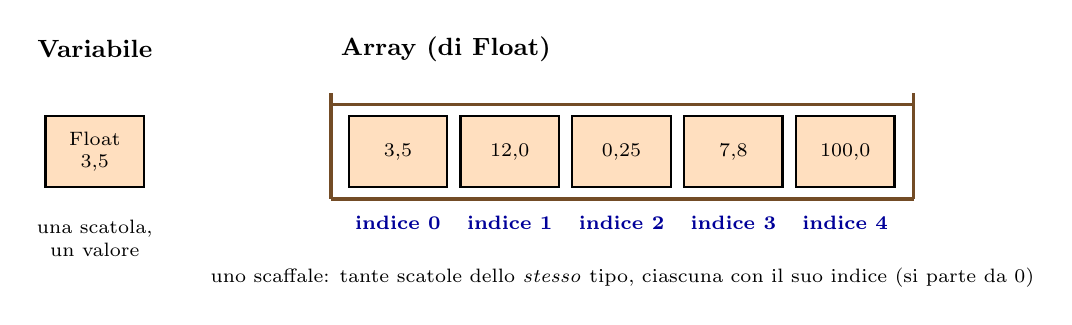
\begin{tikzpicture}[font=\footnotesize,
  ue7box/.style={draw, thick, fill=orange!25, minimum width=1.25cm, minimum height=0.9cm,
                 align=center, font=\scriptsize},
  ue7shelf/.style={draw, very thick, brown!60!black}]
  % variabile singola
  \node[font=\small\bfseries] at (0,2.3) {Variabile};
  \node[ue7box] (v) at (0,1.0) {Float\\3,5};
  \node[font=\scriptsize, align=center] at (0,-0.1) {una scatola,\\un valore};
  % array
  \begin{scope}[xshift=3.0cm]
    \node[font=\small\bfseries, anchor=west] at (0,2.3) {Array (di Float)};
    \draw[ue7shelf] (0,0.4) -- (7.4,0.4);
    \draw[ue7shelf] (0,1.6) -- (7.4,1.6);
    \draw[ue7shelf] (0,0.4) -- (0,1.75);
    \draw[ue7shelf] (7.4,0.4) -- (7.4,1.75);
    \node[ue7box] at (0.85,1.0) {3,5};
    \node[ue7box] at (2.27,1.0) {12,0};
    \node[ue7box] at (3.69,1.0) {0,25};
    \node[ue7box] at (5.11,1.0) {7,8};
    \node[ue7box] at (6.53,1.0) {100,0};
    \foreach \x/\i in {0.85/0, 2.27/1, 3.69/2, 5.11/3, 6.53/4} {
      \node[font=\scriptsize\bfseries, text=blue!60!black] at (\x,0.1) {indice \i};
    }
    \node[font=\scriptsize, align=center] at (3.7,-0.6) {uno scaffale: tante scatole
      dello \emph{stesso} tipo, ciascuna con il suo indice (si parte da 0)};
  \end{scope}
\end{tikzpicture}
\caption{La metafora del docente. Una variabile è una scatola che contiene un valore; un
array è uno scaffale che contiene tante scatole dello stesso tipo. Ogni posto dello
scaffale ha un indice, e il primo indice è 0. Schema ricostruito.}
\label{ue7:fig:scaffale}
\end{figure}

\paragraph{Approfondimento: array, set e map.} Romero e Sewell (capitolo 13, ``Data
Structures and Flow Control'') chiamano \textbf{contenitori} (\emph{containers}) le
strutture che raccolgono più valori dello stesso tipo, e nei Blueprint ce ne sono tre.
L'\textbf{array} è una lista ordinata con accesso per \textbf{indice}, ``e gli array
partono sempre dall'indice 0'': con quattro elementi, il primo ha indice 0 e l'ultimo
indice 3, cioè \emph{Length}~$-$~1. Il \textbf{set} è un insieme senza ordine e senza
doppioni, in cui si cerca per valore; la \textbf{map} associa a ogni \emph{chiave} un
\emph{valore} (per esempio il nome di un'arma e le sue munizioni). Sugli array si lavora
con una manciata di nodi: \textbf{Get (a copy)} legge l'elemento a un indice,
\textbf{Set Array Elem} lo modifica, \textbf{Add} aggiunge in fondo, \textbf{Insert}
inserisce a un indice spostando gli altri, \textbf{Length} e \textbf{Last Index} dicono
quanto è lungo, \textbf{Random Array Item} pesca un elemento a caso. Gli autori
avvertono: mai leggere un indice oltre l'ultimo, perché i risultati sono imprevedibili.
La tabella~\ref{ue7:tab:contenitori} riassume i quattro modi in cui una variabile può
essere costituita.

% ---------------------------------------------------------------------
\section{L'ereditarietà: parent e child}
\label{ue7:sec:ereditarieta}

La slide successiva riprende rapidamente le collisioni (``ripasseremo anche un po' le
collisioni'') e introduce il secondo concetto della giornata. ``Qualcuno di voi ha mai
sentito parlare dei concetti di \textbf{parent} e \textbf{child} in programmazione?''

\paragraph{Padre e figlio.} ``Mettiamo un esempio che possiamo vedere nella vita di tutti
i giorni'': il rapporto fra genitori e figli. ``Io, come figlio di mio padre, ho preso
una parte dei geni di mio padre'' (e di mia madre), ``e però, come essere unico, posso
variare nelle mie particolarità: non sono uguale, ma condivido comunque delle cose''.
Lo stesso succede con gli oggetti: ``ci sono degli oggetti che possono essere figli di
altri oggetti''. Esempio: un cubo \emph{parent} che nel Begin Play stampa un valore, e
fa solo quello. ``Il child mi stamperà sempre quel valore, ma magari stampa anche un
altro valore'': ``prende la caratteristica del papà, ma volendo può aggiungere, o
addirittura \textbf{sovrascrivere}, alcune azioni''.

\paragraph{Il cubo che diventa cilindro.} In Unreal i child si creano direttamente
dall'engine. In slide c'è il BP\_Cube delle lezioni precedenti: ``vogliamo farlo
diventare un cilindro? Creiamo un child e cambiamo semplicemente la Static Mesh''. ``Il
parent rimarrà un cubo, invece il figlio ha voluto cambiare forma'': per le
caratteristiche di Blueprint avranno lo stesso comportamento, ``oppure, volendo, lo
possiamo anche cambiare''. La figura~\ref{ue7:fig:gerarchia} mostra la gerarchia che si
costruirà oggi.

\begin{figure}[htbp]
\centering
\begin{tikzpicture}[font=\footnotesize,
  ue7cls/.style={draw, thick, rounded corners=4pt, align=center, fill=gray!8,
                 text width=3.3cm, minimum height=1.0cm, inner sep=4pt},
  ue7inh/.style={-{Triangle[open, length=3mm, width=3mm]}, thick}]
  \node[ue7cls, fill=gray!20] (actor) at (0,3.0) {\textbf{Actor}\\(classe di Unreal)};
  \node[ue7cls, fill=blue!10] (act) at (0,1.0) {\textbf{BP\_Activable}\\eventi
    Activation e Deactivation (Print String)};
  \node[ue7cls, fill=yellow!25] (light) at (-4.4,-1.4) {\textbf{BP\_ActivableLight}\\Point
    Light; override: accende e spegne};
  \node[ue7cls, fill=green!12] (ball) at (0,-1.4) {\textbf{BP\_BallMoving}\\(esercizio)
    override: Play e Reverse};
  \node[ue7cls, fill=orange!15] (plat) at (4.4,-1.4) {\textbf{piattaforma
    attivabile}\\(esercizio e compito)};
  \node[ue7cls, fill=gray!8] (btn) at (5.2,3.0) {\textbf{BP\_Button}\\array
    ActivableItems di tipo BP\_Activable};
  \draw[ue7inh] (act) -- (actor);
  \draw[ue7inh] (light.north) -- ++(0,0.6) -| (act.south);
  \draw[ue7inh] (ball) -- (act);
  \draw[ue7inh] (plat.north) -- ++(0,0.6) -| (act.south);
  \draw[ue7inh] (btn) -- (actor);
  \draw[-{Stealth[length=2.2mm]}, thick, dashed, violet!60!black] (btn.south) to[bend
    left=10] node[pos=0.45, right, font=\scriptsize, align=left]{contiene referenze\\a
    qualunque child} (act.east);
\end{tikzpicture}
\caption{La gerarchia di classi costruita nella lezione. Le frecce con la punta vuota
vanno dal child al parent (``eredita da''). BP\_Activable definisce i due eventi comuni;
ogni child li ridefinisce a modo suo. BP\_Button tiene un array di referenze di tipo
BP\_Activable, e quindi può contenere qualunque child. I nomi dei Blueprint
dell'esercizio sono quelli suggeriti dal docente; schema ricostruito.}
\label{ue7:fig:gerarchia}
\end{figure}

\paragraph{Approfondimento: superclasse, sottoclasse e tipo.} Romero e Sewell (capitolo
3, ``Object-Oriented Programming and the Gameplay Framework'') danno la versione
tecnica. Quando si crea un Blueprint, la prima cosa che si sceglie è la sua
\textbf{classe parent} (la \emph{superclasse}); un Blueprint ha \emph{un solo} parent,
ma può avere molti child (\emph{sottoclassi}). Il loro esempio sono le armi: una classe
base \emph{Weapon} con tutto ciò che è comune, e le armi concrete come figlie. Il
vantaggio è doppio. Da un lato, una funzione definita nel parent (\emph{Fire}) può
essere \textbf{ridefinita} (\emph{override}) in ogni child (il fucile a energia spara un
raggio, il lanciarazzi un razzo), e a runtime viene eseguita la versione della classe
effettiva dell'oggetto. Dall'altro, un child \textbf{è anche} del tipo del parent:
un'istanza del lanciarazzi è un \emph{Weapon}, e una variabile o un parametro di tipo
Weapon può contenerla. È esattamente il trucco su cui si regge il pulsante di oggi: una
variabile di tipo \emph{BP\_Activable} potrà contenere una luce, una piattaforma, una
palla, qualunque child degli attivabili. Del resto, ogni Blueprint della lezione è già un
child: BP\_Button ha come parent la classe \emph{Actor}.

% ---------------------------------------------------------------------
\section{La dimostrazione: il pulsante finito}
\label{ue7:sec:demo}

``Andremo a creare un bellissimo pulsantone. Eccolo qua.'' Nella scena del docente c'è
il risultato finale. Il giocatore sale sulla pedana, la pedana si abbassa e
\textbf{accende una luce} (``vedremo anche un pochino di \emph{lighting}''); se scende,
la luce si spegne. Nella stessa scena c'è una piattaforma che reagisce allo stesso
pulsante: ``ho creato una piattaforma di tipologia \textbf{attivabile}'', e luce e
piattaforma ``condividono'' qualcosa, ``sono della stessa classe, ma comportamenti
diversi''. Collegata la piattaforma al pulsante, la pressione accende la luce
\emph{e} manda giù la piattaforma; ``in questo caso ho fatto sì che andasse solo giù'':
quando la piattaforma è in basso ci si sale sopra, e lei torna su; si torna sul
pulsante, e di nuovo giù.

\paragraph{La domanda sull'interazione.} ``Faremo anche le interazioni, tipo premi E per
interagire?'' Sì: la prossima lezione sarà sulle \textbf{animazioni}, con un personaggio
animato, e l'interazione si farà con il \textbf{trace}, ``infatti il trace è collegato
al fatto dell'interazione'': ha interagito o non ha interagito.

\paragraph{Approfondimento: overlap o tasto?} I due modi di attivare qualcosa hanno usi
diversi. L'\emph{overlap} di un volume, quello di oggi, è passivo: scatta perché il
giocatore \emph{è} in un posto (pedane a pressione, trappole, cutscene). L'interazione
con un tasto è attiva: il giocatore guarda un oggetto e preme. Lo schema tipico, che la
lezione annuncia, è un \emph{line trace} dalla telecamera in avanti, eseguito alla
pressione del tasto; se colpisce un actor che ``sa'' interagire, gli si chiama un evento.
Per chiamarlo senza sapere in anticipo che classe abbia l'oggetto colpito si usa di
solito una \textbf{Blueprint Interface} (Romero e Sewell, capitolo 16): una lista di
funzioni senza corpo, che ogni classe interessata implementa a modo suo. È una cugina
dell'ereditarietà vista oggi, utile quando le classi da accomunare non hanno un parent
comune.

% ---------------------------------------------------------------------
\section{Il pulsante: due mesh e una box}
\label{ue7:sec:bottone}

``Allora, ragazzi, vi chiedo se siete pronti con il vostro progettino.'' Prima di
cominciare, la raccomandazione di sempre: tenere il progetto ordinato in
\textbf{cartelle}, ``perché se no un giorno succederà che non ritroverete'' le cose,
``come perdere qualcuno in un centro commerciale il sabato''. Nella cartella
\emph{Blueprint}, ``siamo al solito'': Blueprint Class, Actor. Il docente lo chiama
\textbf{BP\_Button1} (``io farò sempre il mio bellissimo BP\_Button1''); nel capitolo è
BP\_Button.

\paragraph{Due Static Mesh, non una.} ``Il bottone, per come sono fatte le mesh, sono due
Static Mesh'': una è il \textbf{frame}, la cornice, e l'altra la \textbf{piastra} che si
abbassa. Il docente le crea con Ctrl+C e Ctrl+V da un componente Static Mesh, e le
rinomina \textbf{Frame} e \textbf{Platform}; nel campo \emph{Static Mesh} assegna alla
prima la mesh della cornice della pedana a pressione (``se non sbaglio \emph{pressure
plate frame}'') e alla seconda quella della piastra (``\emph{pressure plate}\ldots{}
platform''); i nomi esatti degli asset nel progetto del corso non sono sicuri dalla
trascrizione. ``Essendo che sono fatti all'unisono'', i due pezzi sono già allineati.

\paragraph{Un consiglio per i 3D artist.} Il motivo della divisione vale per chiunque
modelli, o faccia modellare, oggetti interattivi. ``Se dovete fare un pulsante, non fate
fare un pulsante unico: fate fare un pulsante che è diviso'' fra la cornice (``quello che
sta attorno'') e la \emph{pressure plate}. ``Perché se adesso andiamo ad abbassare, ed è
un unico asset, tutto il bottone va giù, anche il frame, quindi si va a compenetrare col
pavimento.'' La regola: ``se ci sono delle cose interagibili a livello di movimentazione,
sappiate che è meglio sempre \textbf{splittarle}''. Poi, certo, ``dipende dalla
creatività'' e dal designer.

\paragraph{La box.} Terzo componente, ``la mitica'' \textbf{Box Collision}, scalata
perché sia ``leggermente unanime'' con il bottone, cioè della sua stessa impronta, e
alzata sull'asse Z: ``ricordatevi, attenzione a sotto''. E soprattutto, come per la
piattaforma della volta scorsa, \textbf{figlia della Platform}: ``la box deve seguire la
platform. Importante, in modo tale che se io sposto, si sposta con essa''
(figura~\ref{ue7:fig:bottone}).

\paragraph{È la box a comandare.} Una studentessa chiede conferma: ``bisogna fare la box
sopra perché è la box che interagisce, giusto?'' Sì: il player entra con i piedi nella
box, la box interagisce, la timeline parte e il pulsante va giù. ``Non è tanto la
piattaforma o il pulsante a triggerare l'evento, ma la box sopra.'' E perché non usare
l'overlap della mesh stessa? ``Perché le collisioni sono \textbf{troppo precise}'': sono
``a contatto con una superficie'', ``un controllo sempre più micro'', ``forse sì, forse
no'', e ``la possibilità di errore è molto più ampia''. Un volume, invece, dà una
risposta macro: ``sì, no''.

\begin{figure}[htbp]
\centering
\begin{tikzpicture}[font=\footnotesize,
  ue7comp/.style={draw, thick, rounded corners=3pt, align=left, fill=gray!8,
                  minimum height=0.6cm, text width=3.4cm, inner sep=4pt},
  ue7tree/.style={thick, gray!70!black}]
  \node[font=\small\bfseries, anchor=west] at (-0.2,1.0) {Components di BP\_Button};
  \node[ue7comp, anchor=west] (root) at (0,0.2) {DefaultSceneRoot};
  \node[ue7comp, anchor=west, fill=gray!20] (fr) at (0.6,-0.6) {\textbf{Frame}
    (Static Mesh)};
  \node[ue7comp, anchor=west, fill=blue!10] (pl) at (0.6,-1.4) {\textbf{Platform}
    (Static Mesh)};
  \node[ue7comp, anchor=west, fill=green!12] (bx) at (1.2,-2.2) {\textbf{Box} (Box
    Collision)};
  \node[ue7comp, anchor=west, fill=red!10] (tl) at (0,-3.0) {\textbf{PushButton}
    (Timeline)};
  \draw[ue7tree] (0.2,-0.1) |- (fr.west);
  \draw[ue7tree] (0.2,-0.1) |- (pl.west);
  \draw[ue7tree] (0.8,-1.7) |- (bx.west);
  % vista laterale
  \begin{scope}[xshift=7.4cm, yshift=-1.3cm]
    \draw[thick, gray] (-1.2,-1.0) -- (4.4,-1.0);
    \node[font=\scriptsize, gray] at (3.9,-1.25) {pavimento};
    \fill[gray!45, draw=black, thick] (-0.1,-1.0) rectangle (3.1,-0.75);
    \node[font=\scriptsize] at (1.5,-1.25) {Frame};
    \fill[blue!25, draw=blue!50!black, thick] (0.2,-0.75) rectangle (2.8,-0.5);
    \draw[thick, dashed, blue!50!black] (0.2,-0.85) rectangle (2.8,-0.6);
    \node[font=\scriptsize, anchor=west] at (3.2,-0.55) {Platform};
    \draw[-{Stealth[length=1.6mm]}, thick, red!60!black] (1.5,-0.45) -- (1.5,-0.72);
    \node[font=\scriptsize, red!60!black, anchor=west] at (1.6,-0.25) {$-10$ su Z};
    \draw[thick, dashed, green!50!black, fill=green!8, fill opacity=0.6]
      (0.3,-0.5) rectangle (2.7,0.15);
    \node[font=\scriptsize, green!40!black] at (1.0,-0.17) {Box};
    % omino
    \draw[thick] (-0.7,0.35) circle (0.13);
    \draw[thick] (-0.7,0.22) -- (-0.7,-0.35);
    \draw[thick] (-0.7,-0.35) -- (-0.85,-1.0);
    \draw[thick] (-0.7,-0.35) -- (-0.55,-1.0);
    \node[font=\scriptsize] at (-0.7,0.7) {player};
  \end{scope}
\end{tikzpicture}
\caption{I componenti del pulsante. A sinistra la gerarchia: Frame e Platform sono due
Static Mesh separate; la Box Collision è figlia della Platform, così la segue; la
timeline PushButton compare tra i componenti. A destra la vista laterale: la piastra
scende di 10 unità dentro la cornice (tratteggio), mentre la cornice resta ferma.
Schema ricostruito; le proporzioni non sono quelle dell'asset.}
\label{ue7:fig:bottone}
\end{figure}

% ---------------------------------------------------------------------
\section{Le collisioni della Static Mesh: simple e complex}
\label{ue7:sec:collisioni}

``Poi, se non sbaglio, su questo asset c'è un problema.'' È quello sollevato a inizio
lezione: il pulsante, come la piattaforma, potrebbe avere ``una collisione un po' tanto
alta'' per il personaggio.

\paragraph{Il Max Step Height.} Nel personaggio del giocatore c'è una variabile,
\textbf{Max Step Height}, ``che non ci permette di andare sopra queste tipologie di
asset'' se sono più alte di un certo valore. Il docente prova sulla sua scena: a lui va
``benissimo'', ``perché guardate cosa ho fatto io per ovviare a questo problema''. A
qualcuno degli studenti il personaggio si blocca con i piedi? Pare di no, ``bene''; ma
``per accortezza'', visto che al docente è capitato, si sistema la collisione della mesh.

\paragraph{Approfondimento: Max Step Height e Walkable Floor.} I due parametri stanno nel
\emph{Character Movement Component} del personaggio. Il \textbf{Max Step Height}
(predefinito 45 unità, cioè 45 centimetri) è l'altezza massima di uno ``scalino'' che il
personaggio può salire camminando, senza saltare; il \textbf{Walkable Floor Angle}
(predefinito 44,765 gradi) è la pendenza massima su cui può camminare. Se il bordo della
collisione di un oggetto supera lo scalino, la capsula del personaggio ci sbatte contro
come contro un muro. Si può alzare lo scalino del personaggio, ma cambia il modo in cui
si muove ovunque; di solito conviene sistemare la collisione dell'oggetto, come fa la
lezione.

\paragraph{L'editor della Static Mesh.} Si seleziona la mesh della piastra e si clicca
sulla ``finestrella blu'', l'icona dell'asset nel campo Static Mesh, per aprire
l'\textbf{editor della Static Mesh}: ``la schermata in cui Unreal fa vedere tutte le
particolarità delle collisioni dell'asset stesso'', ``dati molto più \emph{insight} del
modello''.

\paragraph{Una parentesi sui LOD.} Fra i dati ci sono i \textbf{LOD}, i \emph{level of
detail}: ``quella pratica di abbassare la risoluzione degli asset quando sono distanti,
in modo tale da avere ottimizzazione''. ``Sono tipo a 200 metri da me? Abbassa la
qualità, perché pesa.'' Il corso non li userà, ma è bene sapere che esistono.

\paragraph{Simple e complex.} Dal menù \textbf{Show} in alto si visualizzano le
collisioni dell'asset, e ``ci sono due tipologie di collisioni''.
\begin{itemize}
  \item Le \textbf{simple}, in \textbf{verde}: forme semplici, ``usate per avere
        interazioni di base''. Sono quelle che Unreal usa normalmente quando si mette un
        asset nella viewport, ``per tempi e cose di ottimizzazione''.
  \item Le \textbf{complex}, ``questi lineamenti blu'' (azzurri): la forma esatta del
        modello, triangolo per triangolo. Servono quando ``ci serve l'esatto punto''
        in cui si tocca l'oggetto. Esempio: un \textbf{sistema di scalata}, in cui
        ``devo andare a vedere il punto esatto in cui ho messo la mano'' per tirare su il
        personaggio (``poi ci sono anche alternative'').
\end{itemize}
Le due collisioni si preparano ``durante la modellazione'', e chi segue il corso di 3D
art le vedrà. Ma attenzione: ``se mettete le complex collision su tutti gli asset,
probabilmente potete dire ciao al vostro bellissimo PC'', a meno di ottimizzazioni
parallele. Qui servono le simple.

\paragraph{Modificare la collisione.} La cosa bella è che le collisioni simple si
possono modificare a mano. Cliccando sul ``reticoletto verde'' si possono muovere,
ruotare e scalare come un oggetto qualsiasi. Gli studenti dovrebbero avere una
collisione ``un po' più arzigogolata'', ``con tutti i reticolini''; il docente ha già
modificato la sua. La procedura:
\begin{enumerate}
  \item \textbf{cancellare} la collisione simple esistente, ``quella verde, non quella
        azzurra'';
  \item dal menù \textbf{Collision} aggiungerne una nuova, scegliendo fra
        \textbf{Sphere}, \textbf{Capsule}, \textbf{Box} e le varie \textbf{k-DOP} (10DOP-X,
        Y, Z, 18DOP, 26DOP; nella trascrizione ``10 di OP meno X'');
  \item per il pulsante, \textbf{Box} (``Box Simplified Collision''): ``a noi ci serve
        una scatoletta, è un quadrato alla fine'';
  \item selezionare la box e \textbf{stringerla} ``proprio un'anticchia'', abbassandola,
        dopo aver tolto lo \emph{snap}, ``quasi come se fosse una collisione già
        abbassata''.
\end{enumerate}
Ora il pulsante ``ha una collisione un po' più affondabile''.

\paragraph{Le forme a confronto.} Il docente prova le alternative una per una. La
\textbf{sfera} su una piastra quadrata ``non ci serve assolutamente, perché non è
coerente alla sua forma''. Le \textbf{k-DOP} invece seguono il modello con un numero
crescente di piani: ``sono il livello di dettaglio che la collisione avrà, il livello di
vertici''; ``più vertici ci sono, più le collisioni sono precise, meno spigolose''. Sul
cubetto la 10DOP sulla X, sulla Y e sulla Z danno risultati quasi uguali, con ``piccole
differenze'' di taglio; la 18DOP ``ha fatto gli angoli più precisi''; la 26DOP, ``il
massimo'', taglia anche gli spigoli (figura~\ref{ue7:fig:kdop}).

\paragraph{Un'esperienza di lavoro.} ``A me è capitato con un lavoro che ho fatto.'' Nel
livello c'era una piccola pista, e alcuni asset avevano collisioni ``estremamente
complesse'': il docente e il gruppo di designer hanno dovuto \textbf{cancellare tutte le
collisioni e rifarle} a mano, ``con i cubettini'', per semplificare il lavoro
dell'engine. La morale: le collisioni sono parte del lavoro del level designer, non solo
del modellatore.

\begin{figure}[htbp]
\centering
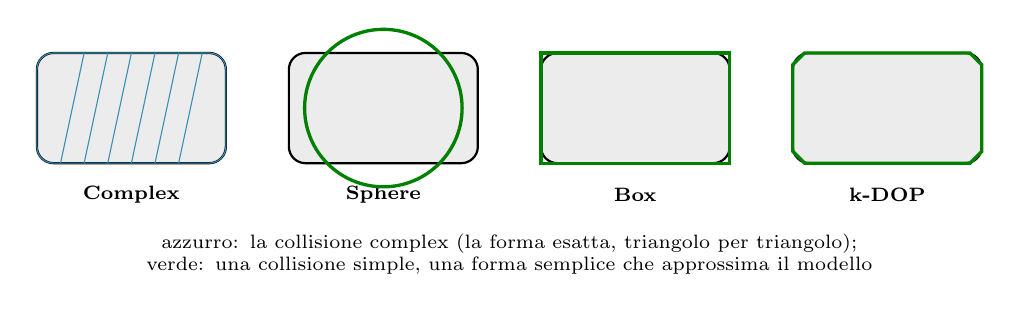
\begin{tikzpicture}[font=\footnotesize,
  ue7mesh/.style={draw=black, thick, fill=gray!15},
  ue7coll/.style={draw=green!50!black, very thick},
  ue7cplx/.style={draw=cyan!70!black, thin}]
  % modello: piastra con bordi smussati (vista dall'alto, stilizzata)
  \foreach \x/\nome in {0/Complex, 3.2/Sphere, 6.4/Box, 9.6/k-DOP} {
    \begin{scope}[xshift=\x cm]
      \draw[ue7mesh, rounded corners=6pt] (0,0) rectangle (2.4,1.4);
      \node[font=\scriptsize\bfseries] at (1.2,-0.4) {\nome};
    \end{scope}
  }
  % complex: segue tutto
  \draw[ue7cplx, rounded corners=6pt] (0,0) rectangle (2.4,1.4);
  \foreach \i in {0.3,0.6,...,2.1} {\draw[ue7cplx] (\i,0) -- (\i+0.3,1.4);}
  % sphere
  \draw[ue7coll] (4.4,0.7) circle (1.0);
  % box
  \draw[ue7coll] (6.4,0) rectangle (8.8,1.4);
  % kdop: ottagono
  \draw[ue7coll] (9.75,0) -- (11.85,0) -- (12.0,0.15) -- (12.0,1.25) -- (11.85,1.4)
    -- (9.75,1.4) -- (9.6,1.25) -- (9.6,0.15) -- cycle;
  \node[font=\scriptsize, align=center, text width=12cm] at (6.0,-1.15) {azzurro: la
    collisione complex (la forma esatta, triangolo per triangolo); verde: una collisione
    simple, una forma semplice che approssima il modello};
\end{tikzpicture}
\caption{Collisioni della piastra viste dall'alto, in forma stilizzata. La complex
segue ogni triangolo del modello; la Sphere non è coerente con la forma; la Box è la
scelta della lezione; le k-DOP aggiungono piani e smussano gli spigoli. Schema
ricostruito, non una schermata dell'editor.}
\label{ue7:fig:kdop}
\end{figure}

\paragraph{Approfondimento: Collision Complexity.} Nell'editor della Static Mesh, fra
i dettagli dell'asset, c'è l'impostazione \textbf{Collision Complexity}. Con il
valore predefinito (\emph{Project Default}, in pratica ``simple e complex separate'') le
query fisiche e il movimento dei personaggi usano la collisione simple, mentre i trace
che lo chiedono esplicitamente (il flag \emph{Trace Complex}) usano quella complex. Con
\emph{Use Complex Collision As Simple} la forma esatta viene usata per tutto: comodo per
un pavimento irregolare statico, ma costoso, e incompatibile con la simulazione fisica
dell'oggetto. Le k-DOP (\emph{discrete oriented polytope}) sono poliedri convessi che
racchiudono la mesh con 10, 18 o 26 piani a orientamento fisso; il menù
\emph{Collision} offre anche \emph{Auto Convex Collision}, che scompone la mesh in più
pezzi convessi, una via di mezzo fra la precisione della complex e il costo della
simple.

% ---------------------------------------------------------------------
\section{La timeline del pulsante}
\label{ue7:sec:timeline}

``Fatto questo, ritorniamo sul nostro bellissimo button e andiamo effettivamente a creare
quello che sarà il funzionamento di base'': il tasto si deve abbassare sulla Z.

\paragraph{Gli eventi e il controllo sul player.} ``Quello che abbiamo visto l'altra
volta'': con la Box selezionata, nella sezione degli eventi in fondo ai dettagli, si
creano \textbf{On Component Begin Overlap} e \textbf{On Component End Overlap}, ``tutti e
due''. Poi ``la solita cosa'': si verifica che sia il player, ``con Is Valid o con il
tag, ma noi facciamo più semplice''. Dall'\textbf{Other Actor} si tira fuori un
\textbf{==} (``uguale uguale'') con \textbf{Get Player Pawn}, e il risultato va in un
\textbf{Branch}.

\paragraph{La timeline.} Dal ramo True, ``abbiamo già detto che è una timeline quella
che useremo'': una nuova timeline, rinominata \textbf{PushButton}, avviata con
\textbf{Play from Start} (la differenza con Play si chiarirà nella
sezione~\ref{ue7:sec:play}). Quanto deve scendere il pulsante? Il docente lo misura
nella viewport: seleziona la piastra, attiva lo \emph{snap} (``molto meglio''), con passo
10, e la abbassa finché è ``totalmente abbassata''. Bastano \textbf{10 unità}: ``quindi
abbiamo capito che dovremmo abbassarla di 10''.

\paragraph{La curva.} Doppio clic sulla timeline. ``Il valore da mettere per la
lunghezza della timeline è \textbf{0,25 secondi}. È molto corto.'' Poi:
\begin{enumerate}
  \item una \textbf{float track};
  \item un punto (Shift e clic) a \textbf{tempo 0, valore 0};
  \item un secondo punto a \textbf{tempo 0,25} (``il massimo della nostra timeline'') e
        \textbf{valore $-$10}: ``farà un passaggio in 0,25 secondi da 0 a $-$10'';
  \item i due pulsantini \textbf{Zoom to Fit Horizontal} e \textbf{Zoom to Fit
        Vertical} (``le due freccine''), che adattano il grafico alla lunghezza e
        all'altezza della curva.
\end{enumerate}
Una domanda dalla chat (``come si chiama il pallino sulla timeline?'') riceve la risposta
già nota: Shift e clic. Rispetto alla piattaforma della volta scorsa c'è una differenza
importante: allora la traccia andava da 0 a 1 ed era un \emph{alfa} da dare a un Lerp;
oggi la traccia contiene \emph{direttamente} lo spostamento, in unità del mondo.

\paragraph{Il nome della traccia.} ``Abbiamo la New Track 0'': la si rinomina cliccandoci
sopra con \textbf{F2}, \textbf{PushButtonZ} (``facciamo una Z maiuscola''). Il pin sul
nodo prende lo stesso nome; a una studentessa resta scritto \emph{New Track 0} anche
dopo la rinomina, e il docente la rassicura: ``è solo il nome che gli abbiamo dato'', il
funzionamento non cambia.

\paragraph{Il movimento.} Nell'Event Graph:
\begin{itemize}
  \item dal pin \textbf{PushButtonZ} si crea un \textbf{Make Vector}, collegando il
        valore alla \textbf{Z} (``l'asse che ci interessa''); X e Y restano a 0, ``tanto
        la X è zero e rimane zero'';
  \item si trascina la Platform nel grafo e se ne tira fuori \textbf{Set Relative
        Location}, con il vettore in \emph{New Location}. ``È relative perché è
        relativa alla sua transform'': lo zero è quello della piastra dentro il
        Blueprint, non lo zero del mondo;
  \item il nodo va collegato all'\textbf{Update} della timeline.
\end{itemize}
In Play, sulla pedana, ``non esplode, vedete che si abbassa''. Ma non si rialza più:
``è normale''. Manca il ritorno: dall'\textbf{End Overlap}, con lo stesso controllo sul
player, si collega l'ingresso \textbf{Reverse} della timeline. ``Premuto, torna su;
premuto, torna su.'' ``Eccolo che abbiamo creato il nostro movimento del pulsante, non
ancora la sua funzionalità'' (figura~\ref{ue7:fig:grafobottone}).

\begin{figure}[htbp]
\centering
\begin{tikzpicture}[font=\footnotesize,
  ue7node/.style={draw, thick, rounded corners=4pt, align=center, fill=gray!8,
                  minimum height=0.8cm, text width=2.0cm},
  ue7ev/.style={ue7node, fill=red!12},
  ue7exec/.style={-{Stealth[length=2.5mm]}, very thick, black!80},
  ue7data/.style={-{Stealth[length=2mm]}, thick, violet!60!black}]
  \node[ue7ev, text width=2.6cm] (bo) at (0,1.2) {\textbf{On Component Begin
    Overlap} (Box)};
  \node[ue7ev, text width=2.6cm] (eo) at (0,-1.2) {\textbf{On Component End
    Overlap} (Box)};
  \node[ue7node, text width=1.9cm] (eq1) at (3.3,2.6) {Other Actor \textbf{==} Get
    Player Pawn};
  \node[ue7node, text width=1.3cm] (br1) at (3.3,1.2) {\textbf{Branch}};
  \node[ue7node, text width=1.3cm] (br2) at (3.3,-1.2) {\textbf{Branch}};
  \node[ue7node, text width=1.9cm] (eq2) at (3.3,-2.6) {Other Actor \textbf{==} Get
    Player Pawn};
  \node[ue7node, fill=red!8, text width=2.4cm, minimum height=2.6cm] (tl) at (7.3,0)
    {\textbf{Timeline}\\PushButton\\[2pt]\scriptsize 0,25 s\\da 0 a $-$10};
  \node[ue7node, text width=1.6cm] (mv) at (10.6,-1.4) {\textbf{Make Vector}\\X 0, Y 0};
  \node[ue7node, text width=2.3cm] (set) at (13.1,0.8) {Platform $\rightarrow$
    \textbf{Set Relative Location}};
  \draw[ue7exec] (bo) -- (br1);
  \draw[ue7exec] (eo) -- (br2);
  \draw[ue7data] (eq1) -- (br1);
  \draw[ue7data] (eq2) -- (br2);
  \draw[ue7exec] (br1.east) -- node[above, font=\scriptsize]{True} ++(0.7,0) |-
    node[pos=0.78, above, font=\scriptsize]{Play from Start} ([yshift=0.8cm]tl.west);
  \draw[ue7exec] (br2.east) -- node[below, font=\scriptsize]{True} ++(0.7,0) |-
    node[pos=0.78, below, font=\scriptsize]{Reverse} ([yshift=-0.8cm]tl.west);
  \draw[ue7exec] ([yshift=0.8cm]tl.east) -- node[above, font=\scriptsize]{Update}
    (set.west);
  \draw[ue7data] ([yshift=-0.6cm]tl.east) -- node[above, font=\scriptsize, pos=0.5]{PushButtonZ}
    ++(0.6,0) |- (mv.west);
  \draw[ue7data] (mv.east) -| node[pos=0.3, below, font=\scriptsize]{Z $\rightarrow$
    New Location} (set.south);
\end{tikzpicture}
\caption{Il movimento del pulsante. Il Begin Overlap della Box, se l'actor è il player,
fa partire la timeline PushButton da capo; l'End Overlap la manda in Reverse. A ogni
Update il valore della traccia (da 0 a $-$10 in 0,25 secondi) diventa la Z di un
vettore, e la piastra si sposta con Set Relative Location. Schema ricostruito.}
\label{ue7:fig:grafobottone}
\end{figure}

\paragraph{Approfondimento: perché qui niente Lerp.} La sesta lezione aveva mostrato il
metodo ``giusto'' per la piattaforma: una traccia da 0 a 1 usata come alfa di un Lerp
fra due posizioni salvate. Qui il docente sceglie la strada diretta, e funziona per due
ragioni. La prima: il valore della traccia è \emph{assoluto}, non si somma alla posizione
corrente, quindi non si accumula (era il difetto del primo metodo della volta scorsa).
La seconda: la piastra è figlia di una radice ferma, e la sua posizione relativa di
partenza è (0, 0, 0), quindi ``$-$10 rispetto alla radice'' vuol dire esattamente ``10
più in basso di dove sta''. Se la piastra fosse stata spostata nel Blueprint, per
esempio a Z 5, il primo Update la teletrasporterebbe a Z 0: in quel caso serve sommare
lo spostamento alla posizione iniziale salvata, o tornare al Lerp. Per oggetti che si
spostano di poco, una traccia in unità del mondo è la soluzione più leggibile.

% ---------------------------------------------------------------------
\section{Le curve: linear e auto}
\label{ue7:sec:curve}

``Adesso vi faccio vedere anche una particolarità, che potremmo usare anche per la
piattaforma'': si può \textbf{modificare la tipologia dei punti}.

\paragraph{Lineari.} I punti creati finora sono \textbf{lineari}: ``formano una linea'',
e l'aumento o la diminuzione del valore ``è sempre costante'' nel tempo: in ogni
frazione di secondo il valore cambia sempre della stessa quantità, ``tra un punto e
l'altro''.

\paragraph{Curve.} ``Se invece vogliamo una curva un po' più \emph{smooth}'', si fa tasto
destro su un punto: compare la serie di \textbf{Key Interpolation}, ``cioè ti dice: quale
tipo di punto vuoi che sia?''. Il docente sceglie \textbf{Auto}, e la linea diventa una
curva; lo stesso sull'altro punto. Ora, con i ``piccoli braccetti'' (le tangenti) di
ciascun punto, si può modellare ``come nel tempo questa linea va da punto A a punto B''
(figura~\ref{ue7:fig:curve}, tabella~\ref{ue7:tab:interp}).

\paragraph{A che cosa serve.} Una studentessa chiede che cosa cambi in pratica. Il
docente prova: allunga la timeline a 1 secondo e piega la curva in modo che superi il
valore finale e poi ci ritorni. Il risultato, con un'escursione di appena 10 unità, sono
``micro movimenti'': il pulsante ``fa boom e ritorna su'', ``su e giù e si abbassa''.
``Cambiare la forma della curva ci permette di creare dei piccoli intervalli di vario
tipo'': il movimento rallenta, accelera, rimbalza. Su un pulsante si vede poco (``è molto
piccolo come spazio''); ``magari in pausa'' il docente propone di mostrarlo con ``una
piccola sferetta che fa su e giù''. Poi rimette la curva com'era.

\begin{figure}[htbp]
\centering
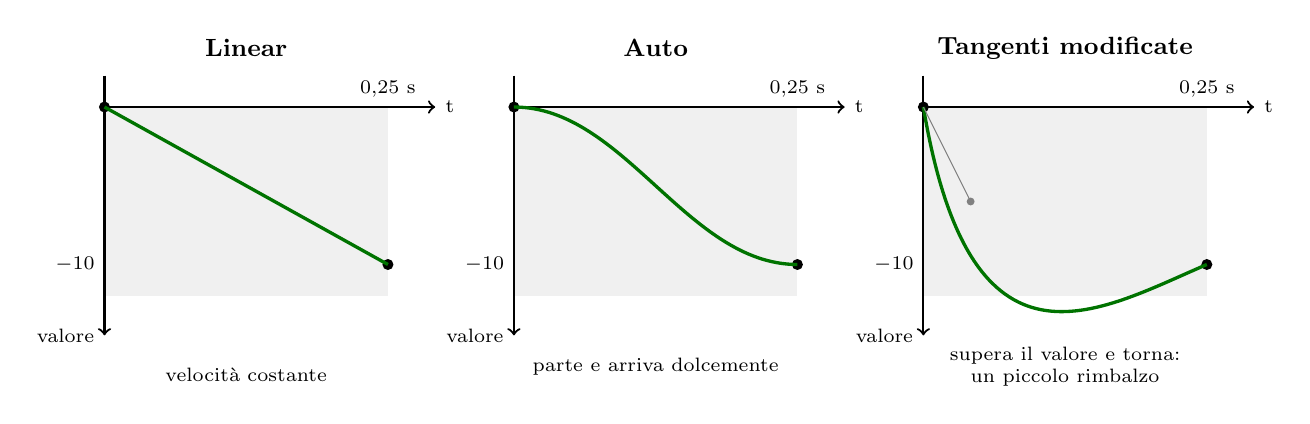
\begin{tikzpicture}[font=\footnotesize]
  \foreach \x/\titolo in {0/Linear, 5.2/Auto, 10.4/Tangenti modificate} {
    \begin{scope}[xshift=\x cm]
      \fill[gray!12] (0,-2.4) rectangle (3.6,0);
      \draw[->, thick] (0,0) -- (4.2,0) node[right, font=\scriptsize]{t};
      \draw[->, thick] (0,0.4) -- (0,-2.9) node[left, font=\scriptsize]{valore};
      \node[font=\scriptsize, left] at (0,-2.0) {$-10$};
      \node[font=\scriptsize, above] at (3.6,0) {0,25 s};
      \node[font=\small\bfseries] at (1.8,0.75) {\titolo};
      \fill (0,0) circle (0.07);
      \fill (3.6,-2.0) circle (0.07);
    \end{scope}
  }
  \draw[very thick, green!45!black] (0,0) -- (3.6,-2.0);
  \draw[very thick, green!45!black] (5.2,0) .. controls (6.6,0) and (7.4,-2.0) ..
    (8.8,-2.0);
  \draw[very thick, green!45!black] (10.4,0) .. controls (11.0,-3.6) and (12.6,-2.6) ..
    (14.0,-2.0);
  \draw[gray, thin] (10.4,0) -- (11.0,-1.2);
  \fill[gray] (11.0,-1.2) circle (0.05);
  \node[font=\scriptsize, align=center] at (1.8,-3.4) {velocità costante};
  \node[font=\scriptsize, align=center] at (7.0,-3.3) {parte e arriva dolcemente};
  \node[font=\scriptsize, align=center] at (12.2,-3.3) {supera il valore e torna:\\un
    piccolo rimbalzo};
\end{tikzpicture}
\caption{La stessa traccia con tre interpolazioni. Con le key lineari il pulsante scende
a velocità costante; con Auto la curva è morbida agli estremi; trascinando le tangenti
(i ``braccetti'') si ottengono andamenti come il rimbalzo provato a lezione. Schema
ricostruito.}
\label{ue7:fig:curve}
\end{figure}

\begin{table}[htbp]
\centering
\small
\begin{tabular}{@{}p{3.0cm}p{11.0cm}@{}}
\toprule
\textbf{Key Interpolation} & \textbf{Andamento fino alla key successiva} \\
\midrule
Auto & curva morbida, con tangenti calcolate in automatico (la scelta della lezione) \\
User & curva morbida con tangenti impostate a mano trascinando i ``braccetti'' \\
Break & come User, ma le due tangenti del punto si muovono in modo indipendente
(spigoli voluti) \\
Linear & retta: variazione costante nel tempo (il comportamento predefinito dei punti
creati con Shift e clic) \\
Constant & il valore resta fermo e salta alla key successiva al suo arrivo (a
gradino) \\
\bottomrule
\end{tabular}
\caption{I tipi di interpolazione di una key, dal menù del tasto destro su un punto della
timeline. La lezione usa Linear e Auto; le altre voci sono un'integrazione basata
sull'editor di Unreal Engine 5.}
\label{ue7:tab:interp}
\end{table}

\paragraph{Approfondimento: \emph{easing} e \emph{game feel}.} Le curve sono lo strumento
più economico per dare \emph{peso} a un movimento. In animazione si parla di
\emph{ease in} e \emph{ease out} (partire e arrivare lentamente) e di
\emph{overshoot} (superare la meta e tornare indietro, come il rimbalzo provato dal
docente): una porta che rallenta prima di chiudersi, un pulsante che affonda di colpo e
risale con un piccolo rimbalzo, un ascensore che parte dolcemente. A parità di durata,
un movimento lineare appare meccanico, uno con l'\emph{easing} appare fisico. Nelle
timeline la curva è anche un \emph{asset} riutilizzabile: dall'editor la traccia si può
salvare come \textbf{Curve Float} esterna e usare in più timeline, così tutti i pulsanti
del gioco si muovono allo stesso modo e si correggono in un punto solo.

% ---------------------------------------------------------------------
\section{I problemi degli studenti con il pulsante}
\label{ue7:sec:problemibottone}

``Il mio bottone non scende.'' ``Neanche a me.'' Il docente ripassa il grafo (Platform,
Set Relative Location sull'Update, il pin della traccia nella Z del Make Vector) e poi
chiama le studentesse in condivisione, una alla volta, ``Lucrezia per prima''. La
condivisione dello schermo su Zoom richiede diversi tentativi, fra permessi da dare,
barre degli strumenti che spariscono e un'eco ``quasi un boomerang''; alla fine
funziona.
\begin{itemize}
  \item \textbf{Il volume.} La box è ``molto piccola'' e il volume ``troppo basso'': deve
        stare sopra la piastra.
  \item \textbf{I punti della curva.} Il primo punto non sta a tempo 0: ``devi mettere
        tempo zero, valore zero''; il secondo a 0,25 e $-$10 ``va benissimo''. E le due
        freccine dello Zoom to Fit aiutano a vedere davvero la curva.
  \item \textbf{La lunghezza.} Un'altra studentessa ha messo 0,25 nel tempo del punto ma
        ha lasciato la \textbf{Length} della timeline al valore predefinito: ``devi
        modificare la lunghezza; vedi, c'è scritto \emph{Length} sopra''.
  \item \textbf{Stop invece di Reverse.} Sull'End Overlap era collegato \emph{Stop}: il
        pulsante si ferma dov'è invece di tornare su.
  \item \textbf{L'Update scollegato.} Il caso più istruttivo: il Set Relative Location
        aveva il pin dei dati collegato, ma non quello di \textbf{esecuzione}
        all'Update. ``Qui devi collegare solo l'execution pin.'' ``Ricordati, fai conto
        che l'Update è quello che fa'' il lavoro nel tempo della linea del tempo.
\end{itemize}
Un consiglio di contorno: ``spostati un po' gli asset'' di prova delle lezioni
precedenti, che potrebbero dare fastidio ai ``grubetti'' (forse i cubetti della
matrice).

\paragraph{Approfondimento: dati senza esecuzione.} L'ultimo errore è il più tipico di chi
viene da altri strumenti. Nei Blueprint i \textbf{pin di dati} (colorati) dicono
\emph{con che cosa} lavora un nodo, i \textbf{pin di esecuzione} (bianchi) dicono
\emph{quando} il nodo viene eseguito. Un nodo con i soli dati collegati non viene mai
eseguito: i suoi ingressi verrebbero calcolati se qualcuno lo chiamasse, ma nessuno lo
chiama. Fanno eccezione i nodi \emph{pure}, senza pin bianchi (come Make Vector o
Get Player Pawn), che vengono calcolati quando un nodo eseguito ne legge l'uscita. Il
controllo da fare quando ``non succede niente'' è quindi sempre lo stesso: seguire il
filo bianco dall'evento fino all'ultimo nodo.

% ---------------------------------------------------------------------
\section{Play o Play from Start?}
\label{ue7:sec:play}

``Posso fare una domanda rapidissima? Perché abbiamo usato Play from Start e non
Play?'' La risposta del docente, con un esempio di timeline da 0 a 2 secondi.
\begin{itemize}
  \item Con \textbf{Play}, se ci si ferma a 1 secondo (si esce dal pulsante quando la
        piastra ``sta a metà'') e poi si rientra, la timeline ``continuerà da quel punto
        in particolare dove ci siamo fermati'': da 1 a 2.
  \item Con \textbf{Play from Start}, se si esce e si rientra, la timeline ``riparte da
        0, non da 1''.
\end{itemize}
Nel caso del pulsante, dice il docente, ``non abbiamo particolari interruzioni, perché
abbiamo proprio un \emph{in} e \emph{out}''.

\paragraph{Approfondimento: che cosa succede davvero con il Reverse.} Con un pulsante
così breve la differenza si nota poco, ma esiste, ed è utile capirla con la
figura~\ref{ue7:fig:play}. Si entra, la timeline va avanti; si esce a metà, e il Reverse
la fa tornare indietro \emph{da dove si trova}. Se si rientra prima che sia tornata a 0:
\begin{itemize}
  \item con \textbf{Play} la timeline inverte di nuovo la direzione dal punto in cui è,
        e la piastra riprende a scendere senza scatti;
  \item con \textbf{Play from Start} la timeline salta a 0: la piastra torna di colpo in
        alto e riparte a scendere, un piccolo scatto visibile.
\end{itemize}
Per oggetti che vanno avanti e indietro seguendo un ingresso e un'uscita (pulsanti,
porte, piattaforme) la coppia più naturale è quindi \textbf{Play} e \textbf{Reverse}; è
proprio quella che il docente raccomanderà nell'esercizio finale
(sezione~\ref{ue7:sec:esercizio}) e che correggerà nella soluzione di uno studente
(``mettilo su Play, non Play from Start''). Play from Start serve quando ogni attivazione
deve ripetere l'animazione da capo, per esempio un colpo o un lampo.

\begin{figure}[htbp]
\centering
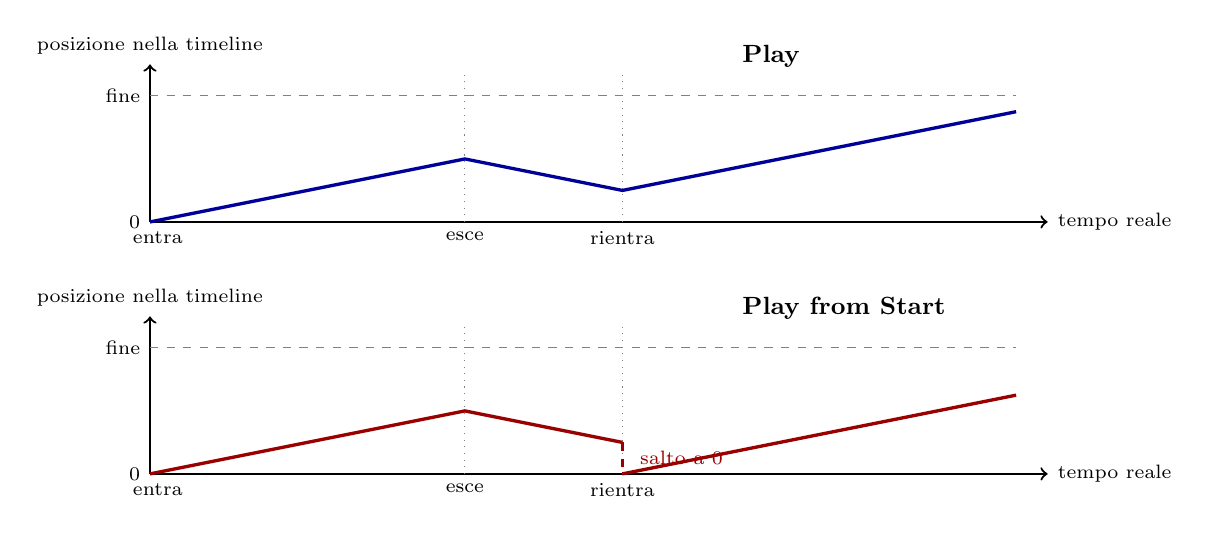
\begin{tikzpicture}[font=\footnotesize, x=1.0cm, y=1.0cm]
  \foreach \y/\titolo in {0/Play, -3.2/Play from Start} {
    \begin{scope}[yshift=\y cm]
      \draw[->, thick] (0,0) -- (11.4,0) node[right, font=\scriptsize]{tempo reale};
      \draw[->, thick] (0,0) -- (0,2.0) node[above, font=\scriptsize]{posizione nella
        timeline};
      \draw[gray, dashed] (0,1.6) -- (11,1.6);
      \node[font=\scriptsize, left] at (0,1.6) {fine};
      \node[font=\scriptsize, left] at (0,0) {0};
      \node[font=\small\bfseries, anchor=west] at (7.4,2.1) {\titolo};
      \draw[gray, dotted] (4,0) -- (4,1.9);
      \draw[gray, dotted] (6,0) -- (6,1.9);
      \node[font=\scriptsize, below] at (0.1,0) {entra};
      \node[font=\scriptsize, below] at (4,0) {esce};
      \node[font=\scriptsize, below] at (6,0) {rientra};
    \end{scope}
  }
  % Play
  \draw[very thick, blue!60!black] (0,0) -- (4,0.8) -- (6,0.4) -- (11,1.4);
  % Play from start
  \draw[very thick, red!60!black] (0,-3.2) -- (4,-2.4) -- (6,-2.8);
  \draw[very thick, red!60!black, dashed] (6,-2.8) -- (6,-3.2);
  \draw[very thick, red!60!black] (6,-3.2) -- (11,-2.2);
  \node[font=\scriptsize, red!60!black, anchor=west] at (6.1,-3.0) {salto a 0};
\end{tikzpicture}
\caption{Entrare, uscire a metà e rientrare prima che la timeline sia tornata a 0. Con
Play (in alto) la timeline riprende da dove si trova; con Play from Start (in basso)
salta all'inizio, e l'oggetto fa uno scatto. Schema ricostruito come integrazione alla
risposta del docente.}
\label{ue7:fig:play}
\end{figure}

% ---------------------------------------------------------------------
\section{Gli attivabili: la classe BP\_Activable}
\label{ue7:sec:activable}

``Adesso andiamo a fare una cosa bellina.'' Il pulsante si muove, ma non fa ancora
niente. Prima di creare la luce, ``prima, importante'', serve una \textbf{tipologia di
actor}: quella degli \textbf{attivabili}, ``quelli che per noi saranno gli attivabili''.

\paragraph{La classe base.} Un nuovo Blueprint Class di tipo Actor: il docente lo chiama
BP\_Activable1, qui è semplicemente \textbf{BP\_Activable}. ``Che succede qui all'interno? Ci serve solo
questo'': con la sola creazione ``abbiamo intanto definito una tipologia di actor''.
Dentro, due \textbf{Custom Event}:
\begin{itemize}
  \item \textbf{Activation}, collegato a un Print String ``attivato'';
  \item \textbf{Deactivation}, collegato a un Print String ``deattivato'' (cioè
        disattivato).
\end{itemize}
``Questi due eventi saranno collegati all'attivare qualcosa o disattivare qualcosa.'' Le
due stampe sono provvisorie: servono a vedere che il collegamento funziona, e poi a
capire come i figli possono \emph{sovrascrivere} gli eventi del padre
(sezione~\ref{ue7:sec:override}).

\paragraph{La domanda.} ``Quando è che io lo devo chiamare? E soprattutto, come faccio a
fargli dire: ehi, bottone, guarda che devi attivare questo esatto elemento?'' La risposta
è una variabile nel bottone, ed è il cuore della lezione.

% ---------------------------------------------------------------------
\section{Il bottone e la lista degli attivabili}
\label{ue7:sec:array}

\paragraph{Una variabile di tipo BP\_Activable.} Nel Blueprint del bottone si crea una
variabile, \textbf{ActivableItems}, e se ne cambia il tipo. ``Questo è molto
interessante, ragazzi: possiamo creare una variabile del tipo di quell'asset che abbiamo
appena creato'': il tipo è \textbf{BP\_Activable}, nella forma \emph{Object Reference}.
Una variabile così non contiene un numero o un testo, ma un \textbf{riferimento} a un
attivabile presente nel livello.

\paragraph{Pubblica.} ``Facciamola \textbf{pubblica}, e si fa con questo
\textbf{occhietto}'' accanto alla variabile. Il docente mette nel livello un
BP\_Activable e seleziona il pulsante: nei Details, in \emph{Default}, ``è apparso
Activable Items''. ``Vuol dire che questa variabile è modificabile dai Details del nostro
editor'', e quindi ``ci permette di avere interazioni dirette con la viewport,
l'ambiente di gioco'': ogni copia del pulsante nel livello può avere i suoi oggetti da
attivare.

\paragraph{Un array.} ``All'inizio di lezione abbiamo parlato degli array'': il pulsante
non deve attivare un oggetto solo, ``ma una moltitudine di oggetti''. Si cambia quindi
non la \emph{tipologia} della variabile, ma la sua \textbf{costituzione} (``cerchiamo di
dividerli'', precisa il docente): accanto al \emph{Variable Type} c'è un'icona (``questo
cilindro, vabbè, un'ellisse'') con una freccetta, e il menù offre \textbf{Single},
\textbf{Array}, \textbf{Set} e \textbf{Map} (tabella~\ref{ue7:tab:contenitori}). Si sceglie
Array, e l'icona della variabile cambia: ``diventa una matrice'', una griglia di
quadratini. ``Adesso abbiamo una variabile array di tipologia BP\_Activable.''

\begin{table}[htbp]
\centering
\small
\begin{tabular}{@{}p{2.4cm}p{5.8cm}p{5.8cm}@{}}
\toprule
\textbf{Costituzione} & \textbf{Che cosa contiene} & \textbf{Esempio} \\
\midrule
Single & un valore solo (la ``scatola'') & la referenza a una sola luce \\
Array & una lista ordinata di valori dello stesso tipo, con indice da 0; ammette
doppioni & gli oggetti attivati dal pulsante (ActivableItems) \\
Set & un insieme di valori unici, senza ordine e senza indice & i nomi degli oggetti
già raccolti \\
Map & coppie chiave--valore, con chiavi uniche & il nome di un'arma e le sue
munizioni \\
\bottomrule
\end{tabular}
\caption{Le quattro costituzioni di una variabile, dal menù accanto al Variable Type.
La lezione usa Single e Array; le descrizioni di Set e Map seguono Romero e Sewell
(capitolo 13).}
\label{ue7:tab:contenitori}
\end{table}

\paragraph{Quando chiamare gli attivabili.} ``Vogliamo che quando il nostro bel bottone
finisce di fare il suo percorso, e si schiaccia'', partano le attivazioni: si usa
l'uscita \textbf{Finished} della timeline. Ma Finished scatta sia alla fine della
discesa sia alla fine della risalita (dopo il Reverse), quindi bisogna sapere ``che
direzione è''. ``Vi ricordate che abbiamo usato lo Switch l'altra volta sulla
Direction?'' Dal pin \textbf{Direction} si crea uno \textbf{Switch on
ETimelineDirection}, collegato al Finished:
\begin{itemize}
  \item \textbf{Forward}: la timeline è andata avanti, il pulsante è schiacciato,
        quindi \textbf{attiva};
  \item \textbf{Backward}: la timeline è tornata indietro, il pulsante è tornato
        ``alla sua posizione di prima'', quindi \textbf{disattiva}.
\end{itemize}

\paragraph{Il For Each Loop.} ``Abbiamo già visto il For Loop. Questo è il \textbf{For
Each Loop}.'' Si prende un \emph{Get} di ActivableItems e se ne tira fuori il ciclo:
``questa esecuzione verrà fatta per ogni elemento dell'array che abbiamo inserito qua
dentro''; ``abbiamo cinque elementi dentro l'array, verrà fatto cinque volte''. Il nodo ha
due uscite di dati: l'\textbf{Array Element}, ``il singolo elemento che ha preso in
considerazione nel momento preciso del ciclo'', e l'\textbf{Array Index}. Dall'Array
Element, che è di tipo BP\_Activable, si può chiamare direttamente l'evento
\textbf{Activation}, collegato al \textbf{Loop Body}. Per il ramo Backward ``i primi due
li prendete, li copiate, li mettete sotto'': stesso Get, stesso For Each Loop, ma con
\textbf{Deactivation} (figura~\ref{ue7:fig:foreach}).

\begin{figure}[htbp]
\centering
\begin{tikzpicture}[font=\footnotesize,
  ue7node/.style={draw, thick, rounded corners=4pt, align=center, fill=gray!8,
                  minimum height=0.8cm, text width=2.0cm},
  ue7var/.style={ue7node, fill=blue!10, rounded corners=8pt},
  ue7ev/.style={ue7node, fill=red!12},
  ue7exec/.style={-{Stealth[length=2.5mm]}, very thick, black!80},
  ue7data/.style={-{Stealth[length=2mm]}, thick, violet!60!black}]
  \node[ue7node, fill=red!8, text width=1.8cm, minimum height=1.8cm] (tl) at (0,0)
    {\textbf{Timeline}\\PushButton};
  \node[ue7node, text width=2.1cm] (sw) at (3.3,0) {\textbf{Switch on
    ETimelineDirection}};
  \node[ue7node, text width=1.9cm] (fe1) at (6.7,1.4) {\textbf{For Each Loop}};
  \node[ue7node, text width=1.9cm] (fe2) at (6.7,-1.4) {\textbf{For Each Loop}};
  \node[ue7var, text width=2.4cm] (g1) at (6.7,3.1) {\textbf{Get}\\ActivableItems};
  \node[ue7var, text width=2.4cm] (g2) at (6.7,-3.1) {\textbf{Get}\\ActivableItems};
  \node[ue7ev, text width=2.1cm] (a) at (10.4,1.4) {Array Element $\rightarrow$
    \textbf{Activation}};
  \node[ue7ev, text width=2.1cm] (d) at (10.4,-1.4) {Array Element $\rightarrow$
    \textbf{Deactivation}};
  \draw[ue7exec] ([yshift=0.4cm]tl.east) -- node[above, font=\scriptsize]{Finished}
    ([yshift=0.4cm]sw.west);
  \draw[ue7data] ([yshift=-0.4cm]tl.east) -- node[below, font=\scriptsize]{Direction}
    ([yshift=-0.4cm]sw.west);
  \draw[ue7exec] (sw.north) |- node[pos=0.25, left, font=\scriptsize]{Forward} (fe1.west);
  \draw[ue7exec] (sw.south) |- node[pos=0.25, left, font=\scriptsize]{Backward} (fe2.west);
  \draw[ue7data] (g1) -- node[right, font=\scriptsize]{Array} (fe1);
  \draw[ue7data] (g2) -- node[right, font=\scriptsize]{Array} (fe2);
  \draw[ue7exec] (fe1) -- node[above, font=\scriptsize]{Loop Body} (a);
  \draw[ue7exec] (fe2) -- node[below, font=\scriptsize]{Loop Body} (d);
\end{tikzpicture}
\caption{Il pulsante chiama gli attivabili. Alla fine della timeline, lo Switch sulla
Direction sceglie il ramo: in avanti (pulsante schiacciato) un For Each Loop chiama
Activation su ogni elemento di ActivableItems; all'indietro (pulsante rilasciato) un
secondo ciclo chiama Deactivation. Schema ricostruito.}
\label{ue7:fig:foreach}
\end{figure}

\paragraph{Riempire l'array.} ``Ci manca ancora una piccola particolarità'': la variabile
è pubblica perché gli oggetti da attivare si scelgono \emph{nel livello}. Si clicca sul
pulsante nella scena, e in \emph{Default} c'è Activable Items: con il \textbf{+} si
aggiungono gli elementi, ``tutti quelli che volete''. Prima, però, un'avvertenza: ``in
informatica si parte non da uno, ma da \textbf{zero}''; ``l'indice 0 è il primo
indice''. Il primo elemento dell'array è l'elemento 0. Per assegnargli un oggetto ci sono
due modi:
\begin{itemize}
  \item il \textbf{menù a tendina}, che elenca ``tutti gli oggetti che puoi ficcarci
        dentro questo array'', cioè tutti i BP\_Activable presenti nel livello, ``perché
        giustamente è quello'';
  \item il \textbf{contagocce} (\emph{pick actor from scene}), ``proprio come su
        Photoshop'': si clicca sull'icona e si passa sopra gli oggetti della scena;
        sugli oggetti di un altro tipo l'editor avvisa che ``non è compatibile'', sul
        BP\_Activable invece ``è compatibile, ci può entrare dentro''. Un clic, ``ecco che
        è apparso''.
\end{itemize}
In Play, sul pulsante: ``attivato''; si scende: ``disattivato''. ``Vi funziona?''

\paragraph{I problemi.} A una studentessa, sul pulsante non compare la voce dell'array:
``basta che vai dove sono le variabili: c'è l'occhietto. Hai l'occhietto chiuso?''. Si
apre l'occhio, si compila (``se no non va''), e la voce compare. Poi bisogna
\textbf{mettere in scena} l'attivabile, se non c'è, e collegarlo con il contagocce
(``c'è la freccettina, c'è questo mouse con dei riquadri, e subito dopo c'è il
contagocce''). ``Sì, funziona. Ottimo.''

``Quindi, ragazzi, adesso abbiamo creato il funzionamento base'', cioè ``la relazione
tra pulsante e oggetto''. L'oggetto non ha ancora particolari funzionalità, ``se non
stampare due frasi'', ``tuttavia la base ce l'abbiamo''.

\paragraph{Approfondimento: la comunicazione diretta.} Quello costruito è ciò che Romero
e Sewell (capitolo 4) chiamano \textbf{Direct Blueprint Communication}: un Blueprint
tiene una variabile referenza a un altro actor, e la usa come \emph{Target} per
chiamarne le funzioni e gli eventi. Il loro esempio è sorprendentemente vicino a quello
della lezione: un \emph{BP\_LightSwitch} con una variabile di tipo Point Light, resa
\textbf{Instance Editable} (l'``occhietto'' del docente: ogni istanza nel livello può
avere un valore diverso), che a ogni overlap del giocatore accende o spegne una lampada
scelta nei Details dal menù a tendina. La lezione fa un passo in più in due direzioni:
la referenza è un \emph{array}, quindi un pulsante comanda molti oggetti; e il tipo è una
classe \emph{parent} scritta da noi, quindi il pulsante non sa e non deve sapere se
l'oggetto è una luce o una piattaforma. Il libro aggiunge un consiglio che vale anche
qui: prima di usare una referenza, controllarla con \textbf{Is Valid}, perché un elemento
dell'array lasciato vuoto nei Details (il \textbf{+} premuto senza scegliere niente)
produrrebbe l'errore ``Accessed None'' visto a inizio lezione. Lo stesso capitolo 13
mostra il For Each Loop proprio su un array di Point Light, ``le lampade di una
stanza''.

% ---------------------------------------------------------------------
\section{Il figlio: BP\_ActivableLight e i due Begin Play}
\label{ue7:sec:child}

``A questo punto andiamo a evolvere questo attivabile in una luce che si accende e si
spegne.'' Ma, attenzione: ``non andiamo a creare un nuovo Blueprint, ma andiamo a creare
un \textbf{figlio} di questo Blueprint, perché vogliamo che condivida la particolarità di
avere le fasi di attivazione e disattivazione''.

\paragraph{Create Child Blueprint Class.} Tasto destro su BP\_Activable nel Content
Browser, \textbf{Create Child Blueprint Class} (``lo trovate tutto sopra''). Unreal
propone un nome con il suffisso \emph{Child}; il docente lo chiama
\textbf{BP\_ActivableLight}. Aprendolo, in alto a destra nell'editor si legge già il
\textbf{Parent class}: ``guarda, questo è il parent, questo è il suo papà; deriva da
questo''. Una studentessa non trova il comando: va fatto con il tasto destro proprio su
BP\_Activable, non sulla pedana.

\paragraph{Event BeginPlay e Parent: BeginPlay.} Aprendo il figlio, al docente compaiono
nel grafo due nodi: \textbf{Event BeginPlay} e, collegato a esso, un nodo
\textbf{Parent: BeginPlay}. Agli studenti no: il docente aveva cancellato il Begin Play
dal parent. La prova: nel parent si rimette un \textbf{Event BeginPlay} (con un Print
String, ``così si vede bene''), e il figlio creato dopo li mostra entrambi. Il
significato: ``io eseguirò il tuo Event BeginPlay assieme all'Event BeginPlay del mio
papà''. ``Va a eseguire in sostanza due Begin Play.''

\paragraph{La dimostrazione.} Nel figlio il Begin Play non contiene niente, a parte la
chiamata al parent; eppure, in Play, la stampa del parent compare. ``Questo è il child.
Qua dentro non c'è un Print String, non c'è niente. Ma lui andrà a fare il Begin Play
del suo papà.'' Se si \textbf{stacca} il nodo Parent: BeginPlay, ``non mi stampa più
niente''. Lo stesso varrebbe per ogni altro evento: ``se dovessimo fare un Event Begin
Overlap, avremmo la stessa identica cosa'', cioè la domanda ``vuoi che ti esegua anche
quello del tuo papà? Sì o no?''. Il nodo si può anche cancellare: ``questo era per
spiegare la \textbf{condivisione degli eventi}''.

\paragraph{Approfondimento: estendere o sostituire.} Il nodo \emph{Parent: BeginPlay} è
la chiave per capire l'override. Quando un child definisce un evento che esiste già nel
parent, la sua versione \emph{sostituisce} quella del parent; il nodo
\emph{Parent:~\ldots}, collegato al filo di esecuzione, la richiama in un punto preciso.
Collegato all'inizio, il child fa prima ciò che fa il parent e poi aggiunge il suo
(\emph{estende}); collegato alla fine, aggiunge prima il suo; scollegato o cancellato, il
child fa solo il suo (\emph{sostituisce}). Unreal lo crea in automatico quando il parent
ha già quell'evento, come gentile promemoria; se manca, si aggiunge con il tasto destro
sul nodo dell'evento, \textbf{Add Call to Parent Function}. Servirà nella
sezione~\ref{ue7:sec:parent}.

% ---------------------------------------------------------------------
\section{La luce: la Point Light}
\label{ue7:sec:luce}

``Andiamo a mettere questa bella lucina.'' Il docente illumina un po' il suo asset ``perché
così non si può vedere'', e aggiunge al figlio un componente \textbf{Point Light}, la luce
puntiforme che illumina in tutte le direzioni: ``la potete vedere che si è creato un
reticolo''. I parametri principali, uno alla volta, in una piccola finestra di prova:
\begin{itemize}
  \item \textbf{Intensity}: ``l'intensità della luce: aumenta, diminuisce'';
  \item \textbf{Attenuation Radius}: il raggio disegnato attorno alla luce, ``quanto si
        espande''; se lo si allarga, il muro vicino viene illuminato;
  \item \textbf{Source Radius}: ``il raggio della sua sorgente'', il ``pallino'' che si
        vede al centro quando si guarda una luce;
  \item \textbf{Soft Source Radius} e \textbf{Source Length} (``la lente, volendo, si
        evolve in verticalità: una specie di lampione tutto strano''), ``una cosa un po'
        più particolare'';
  \item \textbf{Light Color}: con la ruota dei colori, il cursore del chiaro e scuro e
        quello della ``tendenza al bianco'' (la saturazione). Il docente la fa
        \textbf{blu}, ``per differenziarla dall'altra''.
\end{itemize}
L'intensità finale è \textbf{20.000} (il docente dice prima ``200.000'', poi si
corregge: ``20.000, scusate''). ``Questo era semplicemente un piccolo cenno sulle
luci.''

\paragraph{Approfondimento: unità e mobilità delle luci.} In Unreal Engine 5 l'intensità
di una Point Light si misura di solito in \textbf{candele} (o in lumen), e il valore
predefinito di una luce nuova è basso; 20.000 nella vecchia unità adimensionale
(\emph{Unitless}) è invece una luce molto forte, e il numero giusto dipende dall'unità
impostata nel campo \emph{Intensity Units} e dall'esposizione della camera. C'è poi una
condizione per poter cambiare una luce \emph{mentre il gioco gira}: la sua
\textbf{Mobility} deve essere \emph{Movable} (o \emph{Stationary} per intensità e
colore), non \emph{Static}, perché le luci statiche vengono ``cotte'' nelle lightmap e
non esistono più come luci a runtime. Romero e Sewell lo fanno notare nell'esempio del
loro interruttore: la lampada va resa Movable. Con Lumen, il sistema di illuminazione
dinamica predefinito di Unreal Engine 5, le luci sono in genere già Movable.

% ---------------------------------------------------------------------
\section{Salvare l'intensità e sovrascrivere gli eventi}
\label{ue7:sec:override}

``Ci serve, per mettere i due stadi di activation e deactivation, prima di tutto'' un
passaggio nel \textbf{Begin Play}. La luce deve partire spenta, e accendersi poi con
l'intensità scelta nell'editor (20.000). Ma se all'inizio la si spegne, quel numero
andrebbe perso.

\paragraph{IntensityStart.} ``Vi ricordo che tutte le cose che vedete'' nei Details
``sono tutte modificabili, sono tutte richiamabili.'' Dal componente Point Light si tira
fuori \textbf{Get Intensity} (``stiamo prendendo l'intensità attuale'') nel Begin Play,
``all'inizio, quando il frame esiste'', e con \textbf{Promote to Variable} si salva in
una nuova variabile, \textbf{IntensityStart}: ``una variabile di \textbf{appoggio}'',
che serve solo a ricordare il valore da riproporre quando la luce si accenderà. ``Non
serve il Parent: BeginPlay'', aggiunge il docente, ``perché tanto nel parent non facciamo
niente.''

\paragraph{Il problema delle stampe.} Se ora si chiamano gli eventi Activation e
Deactivation sulla luce, la luce ``rimane accesa, è normale'', e in più il figlio
``condividerà il fatto'' di stampare ``attivato'' e ``deattivato'': ha ereditato gli
eventi del padre così come sono. ``Noi non vogliamo questo: noi vogliamo semplicemente
che la luce si spenga.''

\paragraph{L'override.} ``Come facciamo a sovrascrivere questo evento?'' Nel pannello My
Blueprint, accanto a \emph{Functions}, c'è il menù \textbf{Override}: elenca gli eventi
e le funzioni che si possono ridefinire, quelli di Actor (``ActorBeginCursorOver'',
``BeginPlay'', ``Reset'' e così via) e, in fondo, \textbf{Activation} e
\textbf{Deactivation}, ereditati da BP\_Activable. Scegliendoli, compaiono nel grafo del
figlio. ``Che vuol dire override? Vuol dire che stiamo \textbf{sovrascrivendo}'' gli
eventi. Prova: in Play, con i due eventi vuoti, ``non mi fa più niente. È giusto così'':
la versione del figlio ha preso il posto di quella del padre. ``Possiamo sovrascrivere
vari eventi all'interno dei child, in modo tale da facilitarci la differenziazione dei
comportamenti.''

\paragraph{Accendere e spegnere.}
\begin{itemize}
  \item Su \textbf{Activation}: dalla Point Light, \textbf{Set Intensity} (``invece di
        get, set''), con \emph{New Intensity} collegato a \textbf{IntensityStart}.
  \item Su \textbf{Deactivation}: Set Intensity a \textbf{0}.
\end{itemize}
Il Target dei due nodi è la Point Light, ``perché stanno qui'', nel figlio.

\paragraph{L'ordine nel Begin Play.} Resta da spegnere la luce all'avvio: nel Begin Play,
``subito dopo il salvarsi la variabile'', si chiama \textbf{Deactivation}. ``Perché non lo
facciamo prima? Perché se facessimo Deactivation prima, il valore che si salverebbe è
zero'' (figura~\ref{ue7:fig:luce}). In Play: la luce, accesa nell'editor, ``si spegne
perché l'ho disattivata''; si sale sul pulsante, ``adesso si accende''. ``Abbiamo fatto il
nostro bottone con una pre-impostazione tra trigger e triggerato.''

\begin{figure}[htbp]
\centering
\begin{tikzpicture}[font=\footnotesize,
  ue7node/.style={draw, thick, rounded corners=4pt, align=center, fill=gray!8,
                  minimum height=0.8cm, text width=2.0cm},
  ue7var/.style={ue7node, fill=blue!10, rounded corners=8pt},
  ue7ev/.style={ue7node, fill=red!12},
  ue7ov/.style={ue7node, fill=orange!18},
  ue7exec/.style={-{Stealth[length=2.5mm]}, very thick, black!80},
  ue7data/.style={-{Stealth[length=2mm]}, thick, violet!60!black}]
  % begin play
  \node[ue7ev, text width=1.9cm] (bp) at (0,2.2) {\textbf{Event BeginPlay}};
  \node[ue7node, text width=2.1cm] (gi) at (3.6,3.7) {Point Light $\rightarrow$
    \textbf{Get Intensity}};
  \node[ue7var, text width=2.0cm] (set) at (3.6,2.2) {\textbf{Set}\\IntensityStart};
  \node[ue7node, text width=2.0cm] (de) at (7.0,2.2) {\textbf{Deactivation}\\(chiamata)};
  \draw[ue7exec] (bp) -- (set);
  \draw[ue7exec] (set) -- (de);
  \draw[ue7data] (gi) -- (set);
  \node[font=\scriptsize, align=left, anchor=west] at (8.3,2.2) {prima si salva,\\poi
    si spegne};
  % override
  \node[ue7ov, text width=2.0cm] (ac) at (0,0) {\textbf{Activation}\\(override)};
  \node[ue7node, text width=2.3cm] (si1) at (3.6,0) {Point Light $\rightarrow$
    \textbf{Set Intensity}};
  \node[ue7var, text width=1.8cm] (gis) at (7.6,0) {\textbf{Get}\\IntensityStart};
  \draw[ue7exec] (ac) -- (si1);
  \draw[ue7data] (gis) -- node[above, font=\scriptsize]{New Intensity} (si1);
  \node[ue7ov, text width=2.0cm] (dc) at (0,-1.8) {\textbf{Deactivation}\\(override)};
  \node[ue7node, text width=2.3cm] (si2) at (3.6,-1.8) {Point Light $\rightarrow$
    \textbf{Set Intensity}\\New Intensity 0};
  \draw[ue7exec] (dc) -- (si2);
\end{tikzpicture}
\caption{Il grafo di BP\_ActivableLight. Nel Begin Play l'intensità scelta nell'editor
viene salvata in IntensityStart e solo dopo la luce viene spenta; i due eventi ereditati
da BP\_Activable sono sovrascritti (override) e accendono o spengono la Point Light.
Schema ricostruito.}
\label{ue7:fig:luce}
\end{figure}

\paragraph{I problemi.}
\begin{itemize}
  \item A uno studente la luce resta accesa, e in più compaiono ancora le scritte
        ``attivato'' e ``deattivato''. Il docente ripete la sequenza; lo studente ritrova
        l'errore da solo: ``avevo collegato per sbaglio IntensityStart pure a quello
        sotto'', cioè anche al Set Intensity della Deactivation, che quindi riaccendeva la
        luce invece di spegnerla.
  \item A un'altra studentessa, quando preme Play, ``non si vede più la luce'': è
        giusto, la luce parte spenta. Ma poi non si accende, e appare solo la stampa.
        Causa: il pulsante nel livello è ancora collegato al BP\_Activable di prova, non
        alla luce. ``Prendi il contagocce e clicca su BP\_ActivableLight.''
\end{itemize}

\paragraph{Approfondimento: gli eventi di BP\_Activable come contratto.} Il risultato di
queste sezioni è un piccolo esempio di \emph{polimorfismo}, il concetto che Romero e
Sewell illustrano con le armi che ridefiniscono \emph{Fire}. Il pulsante chiama
Activation su ogni elemento dell'array senza sapere che cosa ci sia dentro; ogni oggetto
risponde con la propria versione dell'evento. Per aggiungere al gioco un nuovo oggetto
attivabile (una porta, un ventilatore, una trappola) non serve toccare il pulsante:
basta un nuovo child di BP\_Activable che sovrascriva i due eventi. Il parent fa da
\emph{contratto}: ``chi è attivabile sa rispondere ad Activation e Deactivation''. È anche
il motivo per cui conviene lasciare il parent quasi vuoto: le due stampe di prova sono
utili oggi, ma in un progetto vero un evento del parent che stampa qualcosa finirebbe
per stampare in ogni figlio che non lo sovrascrive.

% ---------------------------------------------------------------------
\section{La pausa e il suono della piattaforma}
\label{ue7:sec:pausa}

``Ragazzi, sono le 5 e mezza.'' Il programma della seconda parte: la piattaforma che si
attiva con il pulsante, ``magari un po' come esercizio'', e ``un altro metodo, che è
quello degli \textbf{event dispatcher}''. ``Ci vediamo al solito orario, 17:55, 18.''

Durante la pausa il docente mantiene la promessa fatta a inizio lezione, e completa con
lo studente rimasto indietro l'\textbf{audio della piattaforma} della sesta lezione, in
condivisione dello schermo. È un ripasso utile, perché raccoglie in un unico passaggio
l'ordine corretto dei nodi.
\begin{enumerate}
  \item Il file audio è già importato e impostato (il docente lo verifica aprendolo).
  \item In fondo al grafo, dopo l'Update della timeline, si toglie il Print String di
        prova e si aggiunge un \textbf{Do Once}.
  \item Dopo il Do Once, \textbf{Spawn Sound at Location}, con la \emph{Location} presa
        da \textbf{Get Actor Location} (``spazio vuoto, tasto destro''), collegata al pin
        arancione e non a quello azzurro, e il suono della piattaforma nel campo
        \emph{Sound}.
  \item Dal \emph{Return Value} (``quel pallino blu''), \textbf{Promote to Variable}:
        \textbf{SoundPlatform}.
  \item Solo ora, dal pin \textbf{Direction} della timeline, lo \textbf{Switch on
        ETimelineDirection}, collegato dopo il Set della variabile (``portalo tutto in
        avanti, oltre quello''): su \textbf{Forward}, SoundPlatform $\rightarrow$
        \textbf{Set Pitch Multiplier} a 1; su \textbf{Backward}, una copia con pitch
        \textbf{0,4}.
  \item Sul \textbf{Finished}: SoundPlatform $\rightarrow$ \textbf{Stop}, e dallo Stop
        il \textbf{Reset} del Do Once.
\end{enumerate}
``Si sente l'audio. A posto, perfetto.'' La registrazione della pausa, per il resto, è
coperta dai soliti blocchi senza senso della trascrizione automatica.

% ---------------------------------------------------------------------
\section{La correzione del pitch}
\label{ue7:sec:pitch}

Alla ripresa, ``una piccola cosa per Filippo'', che a inizio lezione aveva segnalato il
bug del suono. Il problema: lo Switch sulla Direction viene eseguito solo dopo lo spawn
del suono, che grazie al Do Once avviene una volta sola, all'inizio del movimento. Se il
giocatore scende dalla piattaforma mentre sta ancora salendo, la timeline va in Reverse,
ma nessuno rimette il pitch: ``partiva e lo faceva solo una volta, quindi non si trova
mai il pitch''.

La correzione è semplice: ``il pitch del suono va settato in automatico sia se va
backwards, sia se esce dal volume''. Sull'\textbf{End Overlap}, prima del
\textbf{Reverse}, si aggiunge SoundPlatform $\rightarrow$ \textbf{Set Pitch Multiplier}
a \textbf{0,4}: ``nel momento esatto in cui esce dal volume, settiamo il pitch a 0,4'',
``anche se in mezzo alla piattaforma mi lancio''. ``E siamo tranquilli.''

\paragraph{Approfondimento: lo stesso errore, di nuovo.} Il nuovo Set Pitch Multiplier
ha lo stesso rischio dell'errore di inizio lezione: se il giocatore entra ed esce dalla
box prima che la timeline abbia prodotto il primo Update, SoundPlatform è ancora vuota,
e l'End Overlap la usa. In pratica capita di rado, ma una macro \textbf{Is Valid} sulla
variabile, prima del Set, lo esclude del tutto. Più in generale, un suono il cui pitch
deve seguire la direzione del movimento si gestisce meglio leggendo la Direction della
timeline a ogni Update (o, ancora meglio, chiamando Set Pitch Multiplier ogni volta che
si chiamano Play o Reverse), invece che una volta sola all'inizio.

% ---------------------------------------------------------------------
\section{Un altro metodo: gli event dispatcher}
\label{ue7:sec:dispatcher}

``Allora, ragazzi, eravamo rimasti con il nostro bottoncino che ci dava la possibilità di
accendere e spegnere una luce. Possiamo usare questo metodo, però volendo potremmo anche
vedere un altro modo'': gli \textbf{event dispatcher}. Si trovano nel pannello My
Blueprint del bottone, sotto \emph{Variables}, nella sezione \textbf{Event Dispatchers}.

\paragraph{Che cosa sono.} ``Gli event dispatcher, a differenza dei custom event, ci
permettono di \textbf{bindare} vari eventi tra di loro''; ``bindare sta per
collegare''. L'esempio del docente: tre custom event, A, B e C. Con un event dispatcher
si possono legare A, B e C tutti insieme a un altro evento, oppure solo A e C: ``a un
evento di salto succede che si salta; voglio che mi faccia, assieme al salto, A e C''.
Così si tengono separati, per esempio, un controllo e uno sparo, e li si fa partire
insieme quando serve: ``guarda che quando salta, bindami questo evento allo sparo o al
controllo''. ``È un modo un po' più ordinato per fare le cose.'' Lo scopo, oggi, resta lo
stesso: accendere e spegnere la luce con il bottone.

\paragraph{Il dispatcher e il suo parametro.} Con il \textbf{+} accanto a Event
Dispatchers si crea \textbf{OnCheckStatus} (nella trascrizione ``on share status'' e
``check status''; il nome esatto non è del tutto sicuro, ma è quello che il docente usa
nel resto della spiegazione). Come i custom event, anche un dispatcher può avere
\emph{input}: nei Details, con il \textbf{+} della sezione \emph{Inputs}, si aggiunge un
\emph{New Parameter}, rinominato \textbf{IsActive}. Il tipo proposto di base è proprio
il \textbf{Boolean}, ``e va benissimo così'': vero vuol dire che il bottone è attivato,
falso che è disattivato.

\paragraph{A parti invertite.} ``Ma in questo caso andremo a fare una cosa differente.
Invece che il bottone chiami la luce, sarà la luce a controllare lo stato del bottone:
a parti inverse.'' Il pulsante non avrà più bisogno di sapere quali oggetti attivare;
saranno gli oggetti ad \emph{ascoltare} il pulsante. Il docente, per un attimo, stacca
Activation e Deactivation dal resto; poi ci ripensa: ``li useremo comunque in ogni
caso, perdonate''.

% ---------------------------------------------------------------------
\section{La luce si mette in ascolto: Get Actor Of Class e Bind Event}
\label{ue7:sec:bind}

Nel \textbf{Begin Play} di BP\_ActivableLight (dopo il salvataggio dell'intensità) la luce
deve trovare il pulsante e ``attaccarsi'' al suo dispatcher.

\paragraph{Get Actor Of Class.} ``Andiamo a ricercare in tutto il gioco, cioè in tutto lo
spazio di gioco, un attore in particolare.'' Il nodo \textbf{Get Actor Of Class} riceve
una \emph{Actor Class}, qui \textbf{BP\_Button}, e restituisce un actor di quella classe
presente nel livello.

\paragraph{Bind Event.} Dal valore restituito si tira fuori \textbf{Bind Event to
OnCheckStatus}. Il nodo appena creato dà errore: ``è normale, ho fatto compilare prima
del tempo''. Il suo significato, ``letteralmente'': ``attacca un evento''. Quale? Dal pin
rosso \emph{Event} del nodo si tira fuori un filo e si crea un \textbf{Custom Event},
chiamato \textbf{CheckStatusEvent}. ``Guardate la cosa interessante'': il nuovo evento ha
\emph{già} un'uscita \textbf{IsActive}. Un custom event normale nasce vuoto; questo nasce
con la stessa \emph{firma} del dispatcher, ``perché comunque sono in comunicazione'':
``nel check status ci sono questi parametri, che servono alla comunicazione'', e il nodo
li riporta ``nell'evento che tu mi costruisci''. ``Sono due eventi in comunicazione.''

\paragraph{La decisione.} Dentro CheckStatusEvent, ``letteralmente'' un \textbf{Branch}
sul booleano IsActive: se è vero, \textbf{Activation}; se è falso, \textbf{Deactivation}.
Gli eventi sovrascritti della luce restano quelli di prima; cambia solo chi li fa
partire (figura~\ref{ue7:fig:dispatcher}).

% ---------------------------------------------------------------------
\section{Il bottone chiama: Call}
\label{ue7:sec:call}

``La cosa è che il controllo sta dalla parte della nostra carissima luce. Ma come
facciamo a chiamarlo?'' Nel bottone, dopo lo Switch on ETimelineDirection (``subito
dopo, oppure in sostituzione; in questo caso facciamo subito dopo''), si trascina
OnCheckStatus nel grafo. Il menù offre \textbf{Call}, \textbf{Bind}, \textbf{Unbind},
\textbf{Unbind All}, \textbf{Event} e \textbf{Assign}. Si sceglie \textbf{Call}:
``quando succederà questo evento della timeline, che andrà avanti o indietro, chiamami
questo evento e tutti quegli eventi che sono bindati''.
\begin{itemize}
  \item Sul ramo \textbf{Forward}, dopo il For Each Loop delle attivazioni: Call
        OnCheckStatus con \textbf{IsActive vero} (``se è forward, vuol dire che è
        attivo'').
  \item Sul ramo \textbf{Backward}: Call OnCheckStatus con \textbf{IsActive falso}.
\end{itemize}

\paragraph{La prova.} Per dimostrare che il nuovo metodo funziona da solo, il docente
``svuota'' il bottone dalle chiamate dirette: stacca i For Each Loop, lascia collegate
``solamente le due Call, e basta''; nell'array della luce non serve più nulla, ``la
referenza non ci serve''. In Play la luce si accende e si spegne comunque, ``perché sto
eseguendo un check status quando il bottone viene premuto, e lui si ricorda che
all'inizio gli ho collegato quest'altro evento''. ``È come se lo tenesse in memoria.''
``È come dire un \textbf{raggruppamento di eventi}.'' E un'osservazione in risposta a una
perplessità: il Bind è nel Begin Play, ma l'evento non scatta solo nel Begin Play; nel
Begin Play si \emph{stabilisce il legame}, che poi vale ``ogni volta che lo usi''.

\begin{figure}[htbp]
\centering
\begin{tikzpicture}[font=\footnotesize,
  ue7bp/.style={draw, very thick, rounded corners=6pt, inner sep=6pt},
  ue7node/.style={draw, thick, rounded corners=4pt, align=center, fill=gray!8,
                  minimum height=0.8cm, text width=2.1cm},
  ue7ev/.style={ue7node, fill=red!12},
  ue7disp/.style={ue7node, fill=yellow!35},
  ue7exec/.style={-{Stealth[length=2.5mm]}, very thick, black!80},
  ue7link/.style={-{Stealth[length=2.5mm]}, very thick, dashed, red!60!black}]
  % bottone
  \node[ue7node, text width=2.6cm] (sw) at (0,0) {Switch on\\ETimelineDirection};
  \node[ue7disp, text width=2.7cm] (c1) at (3.6,1.1) {\textbf{Call OnCheckStatus}\\IsActive = vero};
  \node[ue7disp, text width=2.7cm] (c2) at (3.6,-1.1) {\textbf{Call OnCheckStatus}\\IsActive = falso};
  \draw[ue7exec] (sw.north) |- node[pos=0.3, left, font=\scriptsize]{Forward} (c1.west);
  \draw[ue7exec] (sw.south) |- node[pos=0.3, left, font=\scriptsize]{Backward} (c2.west);
  \node[ue7disp, text width=2.7cm] (d) at (3.6,-2.9) {Event Dispatcher\\\textbf{OnCheckStatus}\\(IsActive: Boolean)};
  \node[ue7bp, draw=gray!70!black, fit=(sw)(c1)(c2)(d),
        label={[font=\small\bfseries]above:BP\_Button}] (B) {};
  % luce
  \node[ue7ev] (bp) at (9.4,2.4) {\textbf{Event BeginPlay}};
  \node[ue7node, text width=2.2cm] (ga) at (12.4,2.4) {\textbf{Get Actor Of Class}\\BP\_Button};
  \node[ue7node, text width=2.6cm] (bind) at (12.4,0.7) {\textbf{Bind Event to
    OnCheckStatus}};
  \node[ue7ev, text width=2.9cm] (ce) at (9.4,-0.8) {\textbf{CheckStatusEvent}\\(IsActive)};
  \node[ue7node, text width=1.3cm] (br) at (9.4,-2.5) {\textbf{Branch}};
  \node[ue7ev, text width=2.1cm] (ac) at (12.4,-1.8) {\textbf{Activation}};
  \node[ue7ev, text width=2.1cm] (de) at (12.4,-3.2) {\textbf{Deactivation}};
  \draw[ue7exec] (bp) -- (ga);
  \draw[ue7exec] (ga) -- node[right, font=\scriptsize]{Target} (bind);
  \draw[thick, red!70!black, -{Stealth[length=2mm]}] (bind.west) -| node[pos=0.25,
    above, font=\scriptsize]{Event} (ce.north);
  \draw[ue7exec] (ce) -- (br);
  \draw[ue7exec] (br.east) -- ++(0.5,0) |- node[pos=0.8, above, font=\scriptsize]{True} (ac.west);
  \draw[ue7exec] (br.east) -- ++(0.5,0) |- node[pos=0.8, below, font=\scriptsize]{False} (de.west);
  \node[ue7bp, draw=yellow!50!black, fit=(bp)(ga)(bind)(ce)(br)(ac)(de),
        label={[font=\small\bfseries]above:BP\_ActivableLight}] (L) {};
  % il legame
  \draw[ue7link] (c1.east) to[out=0, in=180] (ce.west);
  \node[font=\scriptsize, align=center, red!60!black] at (6.45,-1.6) {la Call\\esegue
    gli\\eventi\\legati};
\end{tikzpicture}
\caption{L'event dispatcher, a parti invertite. Nel suo Begin Play la luce trova il
bottone (Get Actor Of Class) e lega al dispatcher OnCheckStatus un proprio evento,
CheckStatusEvent, che nasce con lo stesso parametro IsActive. Quando il bottone esegue
Call OnCheckStatus, vengono eseguiti tutti gli eventi legati, in qualunque Blueprint si
trovino; la luce decide da sola, con un Branch, se attivarsi o disattivarsi. Schema
ricostruito.}
\label{ue7:fig:dispatcher}
\end{figure}

\paragraph{Approfondimento: dispatcher, ascoltatori e il Level Blueprint.} Romero e
Sewell (capitolo 4, sezioni ``Event Dispatchers'' e ``Binding Events'') descrivono lo
stesso meccanismo con un esempio quasi identico: un \emph{BP\_Platform} che, quando
qualcuno ci passa sopra, esegue \emph{Call} del dispatcher \emph{PlatformPressed}
(con un parametro che passa la referenza a sé stesso, \emph{Self}); il \textbf{Level
Blueprint} si mette in ascolto e fa esplodere qualcosa, e un altro Blueprint, figlio
dell'effetto scintille, lega un proprio custom event allo stesso dispatcher con
\textbf{Bind Event} nel Begin Play, dopo un \textbf{Is Valid} sulla referenza. Due
differenze rispetto alla lezione. La prima: nel libro la referenza al pulsante è una
variabile Instance Editable scelta nei Details, mentre la lezione usa \textbf{Get Actor
Of Class}, che è comodo ma restituisce \emph{il primo} actor di quella classe che trova:
con due pulsanti nel livello, tutte le luci ascolterebbero lo stesso, e quale sia non è
garantito. Per più pulsanti servono una variabile referenza esposta (come nel libro) o
\textbf{Get All Actors Of Class}, che restituisce un array. Inoltre è una ricerca su
tutto il livello, da fare una volta (nel Begin Play, come qui), non a ogni frame. La
seconda: il vantaggio vero del dispatcher è il \textbf{disaccoppiamento}. Chi chiama
(il pulsante) non conosce chi ascolta, e chi ascolta può essere qualunque cosa, anche
un Blueprint che non è un BP\_Activable: un contatore di punteggio, una porta, la musica.
La tabella~\ref{ue7:tab:metodi} confronta i due metodi della lezione.

\begin{table}[htbp]
\centering
\small
\begin{tabular}{@{}p{3.0cm}p{5.5cm}p{5.5cm}@{}}
\toprule
 & \textbf{Array di referenze (primo metodo)} & \textbf{Event dispatcher (secondo
metodo)} \\
\midrule
Chi conosce chi & il pulsante conosce gli oggetti (ActivableItems) & gli oggetti
conoscono il pulsante (Get Actor Of Class) \\
Dove si collega & nei Details del pulsante, con il + e il contagocce & nel Begin Play di
ogni oggetto, con Bind Event \\
Che cosa chiama il pulsante & Activation e Deactivation su ogni elemento, con For Each
Loop & una sola Call di OnCheckStatus, con IsActive \\
Tipo degli oggetti & devono essere child di BP\_Activable & qualunque Blueprint che si
leghi al dispatcher \\
Più pulsanti & ognuno ha il suo array: nessun problema & con Get Actor Of Class
ascoltano tutti lo stesso pulsante \\
Si scollega con & togliendo l'elemento dall'array & Unbind Event (o Unbind All) \\
\bottomrule
\end{tabular}
\caption{I due modi della lezione per far comunicare il pulsante con gli oggetti. Le
ultime due righe sono un'integrazione, non dette a lezione.}
\label{ue7:tab:metodi}
\end{table}

% ---------------------------------------------------------------------
\section{Override, Event e la scatolina}
\label{ue7:sec:scatolina}

Due domande dagli studenti chiudono la spiegazione.

\paragraph{``Perché non compare la stampa del padre?''} ``Quando facciamo l'Activation
della luce, perché non ci compare il print del padre?'' ``Perché quello che abbiamo
fatto prima è stato l'azione di \textbf{override}.'' Il docente la ripete: nel parent,
BP\_Activable, l'evento Activation stampa ``attivato'' e Deactivation ``disattivato'';
nel child, BP\_ActivableLight, l'override ``va a sovrascrivere quell'evento con un nuovo
evento''. Prova del contrario: se nel figlio si cancella l'Activation sovrascritta, il
pulsante torna a stampare ``attivato'', e la luce non si accende più.

\paragraph{``E se volessi fare tutti e due?''} ``Sia quello del padre, sia il suo?'' Qui
il docente improvvisa, e la trascrizione lo segue a fatica: prova a cercare un nodo
\emph{Parent} dal menù contestuale, non lo trova subito (``vediamo un po'\,''), e alla
fine suggerisce una strada alternativa: creare un nuovo custom event (``parent and
child activation'') che \emph{chiami} Activation ``come funzione'', cioè con il nodo
azzurro di chiamata, e subito dopo esegua ciò che il figlio deve aggiungere; ``oppure lo
metti alla fine, direttamente lì'', dopo il CheckStatusEvent. Il metodo standard di
Unreal è più semplice, ed è descritto nella sezione~\ref{ue7:sec:parent}.

\paragraph{``A che cosa serve il check status?''} Un'altra studentessa è tornata indietro:
``il check status mi serve soltanto per evitare il For Each Loop e tutto?''. ``Non
esattamente. Cerco di spiegarmi un po' meglio.'' Il Begin Play, ricorda il docente, è
``quando l'attore incomincia a esistere nel mondo di gioco''. In quel momento la luce ``va
a cercarsi il bottone nel mondo di gioco e gli dice: ehi, c'è un evento che tu chiami
OnCheckStatus; quando viene eseguito, c'è collegato anche questo evento qua''. E propone
di rinominare l'evento in modo più chiaro, per esempio \emph{CheckIfActive}.

\paragraph{La scatolina.} Di nuovo Paint (``bellissima grafia''). ``Immaginatevi una
\textbf{scatolina}: la scatolina è l'evento; è una scatola chiusa per adesso.'' La prima
scatola si chiama \emph{Check} e dentro fa ``tutto quello che gli pare''. Poi c'è un
altro evento, una scatolina più piccola, \emph{Control}, con dentro ``varie operazioni
matematiche''. ``Col binding io la sto aprendo e gli sto dicendo: guarda che quando esegui
questa cosa, mi esegui anche un'altra cosa, e diventa un \textbf{pacchetto completo}.''
Check potrebbe andare dritto al suo risultato, ``ma io gli ho detto: guarda che questo,
quando viene eseguito, deve fare anche Control'' (figura~\ref{ue7:fig:scatolina}).

\paragraph{Unbind.} Dal dispatcher, il menù offre anche \textbf{Unbind}: ``rompimi questo
legame''. La dimostrazione: nella luce, quando si attiva, si esegue \textbf{Unbind Event
from OnCheckStatus} sulla referenza del bottone (con lo stesso CheckStatusEvent come
evento). Risultato: la luce si accende la prima volta, ``ma poi non lo fa più, perché gli
ho rotto il legame''. ``All'inizio è collegato, poi lo stacco, e lui andrà direttamente
all'output'': la scatola Check torna a fare solo il suo contenuto. ``Chiaro?'' ``Sì,
chiaro.''

\begin{figure}[htbp]
\centering
\begin{tikzpicture}[font=\footnotesize,
  ue7scat/.style={draw, very thick, fill=orange!20, rounded corners=2pt, align=center,
                  minimum width=2.6cm, minimum height=1.5cm},
  ue7small/.style={draw, very thick, fill=yellow!30, rounded corners=2pt, align=center,
                  minimum width=1.9cm, minimum height=1.0cm},
  ue7arr/.style={-{Stealth[length=2.5mm]}, very thick}]
  % senza bind
  \node[font=\small\bfseries] at (2.0,2.1) {Senza bind};
  \node[ue7scat] (c1) at (0.6,0.6) {\textbf{Check}\\(il dispatcher)};
  \node[draw, thick, fill=gray!10, rounded corners=3pt] (o1) at (3.5,0.6) {output};
  \draw[ue7arr] (c1) -- (o1);
  \node[ue7small] (k1) at (0.6,-1.2) {\textbf{Control}\\(l'evento)};
  \node[font=\scriptsize, align=center] at (2.9,-1.2) {resta per\\conto suo};
  % con bind
  \begin{scope}[xshift=5.6cm]
    \node[font=\small\bfseries] at (2.4,2.1) {Con Bind: un pacchetto};
    \node[ue7scat] (c2) at (0.6,0.6) {\textbf{Check}};
    \node[ue7small] (k2) at (2.6,0.6) {\textbf{Control}};
    \node[draw, thick, dashed, rounded corners=6pt, fit=(c2)(k2), inner sep=5pt] (pk) {};
    \node[draw, thick, fill=gray!10, rounded corners=3pt] (o2) at (5.0,0.6) {output};
    \draw[ue7arr] (pk) -- (o2);
    \node[font=\scriptsize, align=center] at (2.0,-1.0) {Call esegue Check\\\emph{e} tutto
      ciò che è legato};
  \end{scope}
  % unbind
  \begin{scope}[xshift=12.2cm]
    \node[font=\small\bfseries] at (1.4,2.1) {Dopo Unbind};
    \node[ue7scat] (c3) at (0.6,0.6) {\textbf{Check}};
    \node[draw, thick, fill=gray!10, rounded corners=3pt] (o3) at (0.6,-1.2) {output};
    \draw[ue7arr] (c3) -- (o3);
    \node[ue7small] (k3) at (2.4,-0.3) {\textbf{Control}};
    \draw[very thick, red!70!black] (1.6,0.45) -- (1.9,0.05);
    \draw[very thick, red!70!black] (1.6,0.05) -- (1.9,0.45);
  \end{scope}
\end{tikzpicture}
\caption{La ``scatolina'' disegnata dal docente in Paint. Un evento è una scatola chiusa;
il Bind apre la scatola e ci mette dentro un altro evento, così che chiamarne uno esegua
il pacchetto completo; l'Unbind rompe il legame, e la scatola torna a fare solo il suo
contenuto. Schema ricostruito.}
\label{ue7:fig:scatolina}
\end{figure}

\paragraph{Approfondimento: Bind, Unbind, Unbind All, Assign.} Le voci del menù di un
dispatcher, in sintesi. \textbf{Call} esegue tutti gli eventi legati, nell'ordine in cui
sono stati legati, passando a ciascuno i parametri. \textbf{Bind} aggiunge un evento alla
lista (lo stesso evento legato due volte non viene aggiunto due volte).
\textbf{Unbind} toglie un evento preciso; \textbf{Unbind All} svuota la lista.
\textbf{Assign} è una scorciatoia che crea in un colpo solo il nodo Bind e un custom
event con la firma giusta, quello che il docente fa a mano tirando il filo dal pin
\emph{Event}. Infine \textbf{Event} crea, nel Blueprint che possiede il dispatcher, un
evento già legato. Se l'actor che ascolta viene distrutto, il legame si scioglie da
solo; se invece è il pulsante a sparire, la luce non riceve più nulla, senza errori.

% ---------------------------------------------------------------------
\section{Chiamare anche il parent}
\label{ue7:sec:parent}

La domanda rimasta in sospeso nella sezione~\ref{ue7:sec:scatolina} ha una risposta
diretta, che qui si aggiunge come integrazione alla lezione. Quando un child sovrascrive
un evento del parent, nel grafo del child si fa \textbf{tasto destro sul nodo
dell'evento} (per esempio l'Activation sovrascritta di BP\_ActivableLight) e si sceglie
\textbf{Add Call to Parent Function}. Compare un nodo arancione, \textbf{Parent:
Activation}, identico nello spirito al \emph{Parent: BeginPlay} visto nella
sezione~\ref{ue7:sec:child}. Collegandolo al filo di esecuzione, prima o dopo il Set
Intensity, la luce esegue \emph{sia} la versione del padre (la stampa ``attivato'') sia
la propria (l'accensione). Il metodo del docente, un custom event che chiama Activation e
poi fa altro, raggiunge un effetto simile, ma rischia di confondere: se il nuovo evento
chiama Activation sulla luce stessa, esegue la versione sovrascritta della luce, non
quella del parent.

% ---------------------------------------------------------------------
\section{L'esercizio}
\label{ue7:sec:esercizio}

``Adesso io vi propongo di fare questa cosa come esercizio'', per ``farvi un po'
sperimentare''. Va bene l'uno o l'altro metodo, ``usando il check status, l'event
dispatcher, o il fatto di chiamare gli eventi con l'array''.

\paragraph{La proposta difficile: la piattaforma attivabile.} Creare un \textbf{figlio} di
BP\_Activable (``Create Child Blueprint Class'') e rifare dentro di esso la piattaforma
della sesta lezione, ma comandata dal pulsante: ``vorrei che la piattaforma, invece di
scendere se io overlappo con essa'', si attivi con la pressione del pulsante (``fatela
magari in alto che va in basso, oppure se volete che va in alto, tranquillamente'').
``L'importante è la pressione di un pulsante.'' Il docente spiega come trasportare il
codice.
\begin{itemize}
  \item Si copia il grafo dalla vecchia piattaforma e lo si incolla nel nuovo Blueprint:
        ``vi dirà qualche errore, però è normale'', perché ``queste variabili non
        esistono''.
  \item Ogni variabile mancante si ricrea con il \textbf{tasto destro} sul nodo,
        \textbf{Create Variable}: per esempio Duration. ``Vi consiglio di richiamarla allo
        stesso modo'', e il nodo ``ritorna blu'', cioè valido.
  \item La timeline va chiamata con lo stesso nome della vecchia (Timeline Platform),
        perché i nodi Set Play Rate la cercano per nome.
  \item I componenti vanno riaggiunti a mano: la Static Mesh (``la dovete chiamare allo
        stesso modo'', Platform), il Billboard. Anche la variabile del suono
        (``Somewave'') si ricrea con il tasto destro.
  \item La box \emph{no}: ``non dovete rimettere la box'', perché l'evento che fa partire
        la piattaforma non è più l'overlap, ma l'attivazione da parte del pulsante.
\end{itemize}

\paragraph{Figlio di due padri?} Una studentessa chiede se la nuova piattaforma possa essere ``child di entrambi'':
sia della piattaforma normale, sia dell'attivabile. ``No, purtroppo no.'' Si potrebbe cambiare la
classe parent della vecchia piattaforma, ma ``sicuramente darebbe errori''.

\paragraph{Approfondimento: Reparent Blueprint.} Un Blueprint esistente può effettivamente
cambiare padre: nell'editor, \emph{File} $\rightarrow$ \textbf{Reparent Blueprint}, o il
campo \emph{Parent Class} nelle \emph{Class Settings}. Se il nuovo parent è a sua volta un
Actor (come BP\_Activable), componenti, variabili e grafi della piattaforma restano; gli
errori temuti dal docente nascono quando il nuovo padre non ha qualcosa che il vecchio
aveva, o quando nomi di variabili e di eventi entrano in conflitto. Per la piattaforma,
il reparent a BP\_Activable e l'override di Activation e Deactivation sarebbero una
strada percorribile. L'ereditarietà multipla, invece, nei Blueprint non esiste: per
dare a una classe più ``identità'' si usano le \textbf{Blueprint Interface}.

\paragraph{La proposta facile: un oggetto che si muove.} ``Se no, possiamo fare un
esercizio un po' più semplice'': un Blueprint nuovo, ``\textbf{BP\_BallMoving}, o come vi
pare'', con un oggetto qualsiasi (``un cubo, un cerchio'') che si muove con una timeline e
parte solo quando si preme il pulsante. Le regole:
\begin{itemize}
  \item all'\textbf{attivazione}, la timeline parte: \textbf{Play};
  \item alla \textbf{disattivazione}, la timeline torna indietro: \textbf{Reverse};
  \item sull'Update, si cambia la posizione o la rotazione dell'oggetto, ``destra,
        sinistra, su, giù, come vi pare''.
\end{itemize}
``Quindi è activate, parte la timeline; quando invece finisce, Reverse. Fondamentalmente
è fatto.''

\paragraph{La piattaforma e il Reverse.} ``Ma nel caso della piattaforma non bisogna
usare Reverse, se no quella risale da sola?'' ``Esatto.'' Nella sua versione il docente
ha fatto risalire la piattaforma quando il giocatore ci sale sopra, ``quindi io ce l'ho
messa, la box''. Ma l'esercizio, nella sua forma base, è questo: attivazione, la timeline
va avanti; disattivazione, la timeline va indietro. La classe vota per provarci da sola,
``i più impavidi'' con la piattaforma: venti minuti, poi la correzione.

% ---------------------------------------------------------------------
\section{La soluzione di uno studente}
\label{ue7:sec:soluzione}

``Sarò onesto, non sono convintissimo di come l'ho fatto. Però funziona.'' Uno studente
condivide la sua piattaforma attivabile da un secondo computer. La revisione del docente
è un piccolo catalogo di aggiustamenti.
\begin{itemize}
  \item \textbf{Stop sulla Deactivation.} Lo studente ha messo \emph{Stop} sulla
        disattivazione, così la piattaforma si ferma quando si scende dal pulsante e
        scende solo finché lo si tiene premuto. ``Leva un attimo lo stop sul
        deactivation.''
  \item \textbf{Play, non Play from Start.} il docente chiede di usare Play, non Play from
        Start: la distinzione della sezione~\ref{ue7:sec:play}, ora in pratica.
  \item \textbf{La Duration.} Il play rate copiato dalla vecchia piattaforma usa la
        variabile Duration, che nel nuovo Blueprint vale 0: va messa a \textbf{1} (lo
        studente non ricordava quella parte e voleva cancellarla).
  \item \textbf{Il nome della timeline.} Un nodo non trova la sua timeline: ``la devi
        nominare'' come quella originale, con F2. Compilazione, Play: ``salici sopra.
        Ottimo.''
  \item \textbf{Start e Finish invertite.} Lo studente ha dovuto scambiare Start Location
        e Finish Location per far funzionare il Lerp, e il Billboard ``l'ho messo 300
        sotto''. Il docente all'inizio lo trova giusto, poi no; fa ricreare il
        Billboard, lo fa \textbf{alzare} invece di abbassare, e lo fa ricollegare. Il
        comportamento resta ``strano'' per qualche tentativo, e la causa precisa non
        emerge dalla trascrizione.
  \item \textbf{La curva, di nuovo.} Lo studente pensava di dover invertire la curva
        della timeline, perché la piattaforma parte dall'alto. ``No, è sempre 0--1'':
        ``tu devi dire che lo 0 è la posizione quando stai in alto e 1 la posizione
        quando stai in basso. Questo è il passaggio tra i due, non è alto--basso.'' La
        timeline dice solo ``passi da A a B in un secondo''; chi sia A e chi B lo
        decidono gli ingressi del Lerp.
\end{itemize}
Il suono non c'è ancora: ``ci penso dopo''. Il docente approva, e lascia la regola della
giornata: ``\textbf{sempre ragiona per step}. Fallo funzionare, poi fallo bello.''
``Bravissimo.''

\paragraph{Approfondimento: la timeline come alfa.} L'ultima correzione è la più utile da
fissare. In una timeline usata come alfa di un Lerp, la curva non descrive \emph{dove}
si trova l'oggetto, ma \emph{quanto} del tragitto è stato percorso: 0 è ``alla
partenza'', 1 è ``all'arrivo'', qualunque siano partenza e arrivo. Per una piattaforma che
scende basta mettere in A la posizione alta e in B quella bassa; per una che va di lato,
A e B diversi; la curva resta la stessa. Invertire la curva \emph{e} scambiare A e B
produce lo stesso movimento di partenza (due inversioni si annullano), ma confonde
chiunque legga il grafo, e rende Play e Reverse controintuitivi. La curva va invece
modificata quando si vuole cambiare il \emph{ritmo} (sezione~\ref{ue7:sec:curve}).

% ---------------------------------------------------------------------
\section{Il compito per casa e la chiusura}
\label{ue7:sec:chiusura}

``Mancano tre minuti.'' Chi non ha finito potrà mostrare il lavoro la volta successiva,
o mandarne un video in chat. Il docente chiude due minuti prima, ``così questo esercizio
ve lo portate a casa, anche chi sta in differita'', con il \textbf{compito}: \textbf{la
piattaforma al contrario}.
\begin{enumerate}
  \item Si preme il pulsante: la piattaforma, che sta in alto, \textbf{va giù}.
  \item Si scende dal pulsante: sulla Deactivation \textbf{non succede niente}, la
        piattaforma resta giù.
  \item Si sale sulla piattaforma: \textbf{torna su}.
\end{enumerate}
Si possono usare ``tutti e due i mezzi'': l'event dispatcher, ``oppure la cosa degli
eventi'' chiamati con il ciclo sull'array. ``Va bene, ragazzi. Io vi ringrazio per
l'attenzione. Ci sentiamo per martedì prossimo. Ciao a tutti. Buona serata.''

\paragraph{Approfondimento: una traccia per il compito.} Una possibile struttura, coerente
con la lezione: un child di BP\_Activable, \emph{BP\_ActivablePlatform}, con radice
ferma, Platform, Billboard (figlio della radice) e una Box Collision figlia della
Platform. Nel Begin Play si salvano Start Location (la Platform) e Finish Location (il
Billboard, messo \emph{sotto} la piattaforma). L'override di \textbf{Activation} fa
\textbf{Play} della timeline (alfa da 0 a 1, Lerp da Start a Finish); l'override di
\textbf{Deactivation} resta vuoto; l'\textbf{On Component Begin Overlap} della box, con
il controllo sul player, fa \textbf{Reverse}. Con il secondo metodo, la piattaforma lega
invece un proprio evento all'OnCheckStatus del pulsante, e nel Branch fa Play solo sul
ramo vero. Il suono della sesta lezione si riaggiunge alla fine: prima funzionare, poi
bello.

\begin{table}[htbp]
\centering
\small
\begin{tabular}{@{}p{5.4cm}p{8.6cm}@{}}
\toprule
\textbf{Sintomo} & \textbf{Causa e rimedio} \\
\midrule
``Errore di runtime: accesso nullo'' sul suono, a fine prova & il pitch viene impostato
prima dello spawn del suono: Switch dopo lo Spawn e il Set di SoundPlatform (ed
eventualmente Is Valid) \\
La piattaforma va allo zero del mondo e non torna & manca il DefaultSceneRoot: la mesh è
diventata la radice. Aggiungere un componente Scene e trascinarlo sopra la Platform \\
La piattaforma si sotterra dopo molti passaggi & il Billboard si muove con la parte che
sale: renderlo figlio della radice \\
La piattaforma si riabbassa anche se esce un altro actor & manca il controllo sul player
sull'End Overlap \\
Il player si blocca con i piedi contro la pedana & la collisione è più alta del Max
Step Height: interrare la mesh o rifare la collisione simple (Box, ristretta e
abbassata) \\
Il suono non cambia se si scende a metà salita & il pitch viene impostato solo allo
spawn: Set Pitch Multiplier 0,4 sull'End Overlap, prima del Reverse \\
Il pulsante non scende & box troppo piccola o sotto la piastra; key non a tempo 0;
Length non a 0,25; Update non collegato al Set Relative Location \\
Il pulsante non torna su & End Overlap collegato a Stop invece che a Reverse \\
Il pin della traccia si chiama ancora New Track 0 & solo il nome: non cambia il
funzionamento \\
Activable Items non compare nei Details del pulsante & la variabile non è pubblica:
aprire l'``occhietto'' e compilare \\
Il pulsante stampa ma la luce non si accende & nell'array c'è il BP\_Activable di prova,
non la luce: sceglierla con il contagocce \\
La luce compare in Play ma non si accende, e stampa ancora ``attivato'' & IntensityStart
collegato anche al Set Intensity della Deactivation, o eventi non sovrascritti \\
La luce parte con intensità 0 anche quando si accende & Deactivation chiamata prima di
salvare IntensityStart \\
Nel child non compare Parent: BeginPlay & il parent non ha un Event BeginPlay: il nodo
compare solo se l'evento esiste nel padre \\
Il nodo Bind Event dà errore & si è compilato prima di collegare l'evento: creare il
custom event dal pin Event e ricompilare \\
La luce reagisce solo la prima volta & un Unbind Event eseguito sull'attivazione \\
Errori dopo il copia-incolla del codice della piattaforma & variabili e componenti non
esistono nel nuovo Blueprint: tasto destro, Create Variable; ricreare mesh, Billboard e
timeline con gli stessi nomi \\
La piattaforma attivabile scende solo finché si preme & Stop sulla Deactivation:
toglierlo (e Play invece di Play from Start) \\
Il play rate non ha effetto & Duration a 0 nel nuovo Blueprint: metterla a 1 \\
\bottomrule
\end{tabular}
\caption{I problemi incontrati durante la lezione, con la causa e il rimedio.}
\label{ue7:tab:errori}
\end{table}

\begin{table}[htbp]
\centering
\small
\begin{tabular}{@{}p{4.4cm}p{9.6cm}@{}}
\toprule
\textbf{Nodo, componente o impostazione} & \textbf{Che cosa fa} \\
\midrule
DefaultSceneRoot / Scene & la radice dell'actor; ferma e invisibile, fa da riferimento
per le posizioni relative \\
Static Mesh Editor: Show, Collision & visualizza le collisioni simple (verdi) e complex
(azzurre); aggiunge Sphere, Capsule, Box, k-DOP \\
Max Step Height & altezza massima che il personaggio sale camminando (Character
Movement) \\
Timeline: Length, Key Interpolation & durata della timeline; tipo di curva fra le key
(Auto, User, Break, Linear, Constant) \\
Zoom to Fit Horizontal / Vertical & adatta il grafico della timeline alla curva \\
Play / Play from Start & riprende dal punto attuale; riparte da 0 \\
Make Vector & costruisce un vettore da X, Y, Z \\
Set Relative Location & posizione di un componente rispetto al suo genitore \\
Custom Event & un evento definito da noi, che si chiama per nome \\
Variabile Object Reference & una referenza a un actor di un certo tipo (qui
BP\_Activable) \\
Instance Editable (occhietto) & rende la variabile modificabile nei Details di ogni
istanza del livello \\
Single / Array / Set / Map & la costituzione di una variabile \\
For Each Loop & esegue il Loop Body per ogni elemento di un array (Array Element, Array
Index, Completed) \\
Switch on ETimelineDirection & due uscite: Forward e Backward \\
Contagocce (pick actor) & sceglie dalla scena l'actor da assegnare a una referenza \\
Create Child Blueprint Class & crea un Blueprint figlio, che eredita componenti,
variabili ed eventi \\
Parent: BeginPlay / Add Call to Parent Function & esegue la versione del parent di un
evento sovrascritto \\
Override (My Blueprint) & ridefinisce nel child un evento o una funzione del parent \\
Point Light & luce puntiforme: Intensity, Attenuation Radius, Source Radius, Light
Color \\
Get Intensity / Set Intensity & legge e imposta l'intensità di una luce \\
Promote to Variable & crea una variabile del tipo di un pin e la imposta \\
Event Dispatcher (con input) & un evento a cui altri Blueprint possono legarsi \\
Get Actor Of Class & restituisce un actor di una classe presente nel livello \\
Bind Event / Unbind Event / Unbind All & lega o slega un evento da un dispatcher \\
Call (dispatcher) & esegue tutti gli eventi legati, con i parametri \\
Do Once, Spawn Sound at Location, Set Pitch Multiplier, Stop & il suono della
piattaforma, ripassato in pausa \\
\bottomrule
\end{tabular}
\caption{I nodi, i componenti e le impostazioni della settima lezione.}
\label{ue7:tab:nodi}
\end{table}

% ---------------------------------------------------------------------
\section*{Punti chiave del capitolo}
\addcontentsline{toc}{section}{Punti chiave del capitolo}

\begin{itemize}
  \item Un \textbf{Accessed None} (``accesso nullo'') vuol dire che una referenza è
        vuota quando la si usa: si corregge l'ordine dei nodi e si protegge con
        \textbf{Is Valid}. Un actor ha bisogno di una \textbf{radice} ferma
        (DefaultSceneRoot): se la mesh che si muove diventa la radice, le posizioni
        relative perdono senso.
  \item Un \textbf{array} è uno scaffale di variabili dello stesso tipo, con indice che
        parte da \textbf{0}. La costituzione di una variabile si sceglie accanto al
        Variable Type: Single, Array, Set, Map.
  \item L'\textbf{ereditarietà}: un child eredita componenti, variabili ed eventi del
        parent, può aggiungerne e può \textbf{sovrascriverli} (override). Un child è
        anche del tipo del parent, e una variabile di tipo parent può contenerlo.
  \item Gli oggetti interattivi che si muovono vanno modellati in pezzi separati (cornice
        e piastra). È la \textbf{box} a far scattare l'evento, non la mesh: le collisioni
        della mesh sono troppo precise per un sì o un no.
  \item Le collisioni di una Static Mesh sono \textbf{simple} (verdi, forme semplici,
        usate di base) e \textbf{complex} (azzurre, la forma esatta, costose). Si
        modificano nell'editor della Static Mesh; per una pedana basta una \textbf{Box}
        ristretta e abbassata, sotto il \textbf{Max Step Height} del personaggio.
  \item La timeline del pulsante dura \textbf{0,25 secondi} e va da 0 a $-$10 sulla Z,
        con Make Vector e \textbf{Set Relative Location} sull'Update; l'End Overlap fa
        Reverse. Le key possono essere \textbf{lineari} o curve (\textbf{Auto}, con le
        tangenti), e la curva decide il ritmo del movimento.
  \item \textbf{Play} riprende dal punto attuale, \textbf{Play from Start} riparte da 0:
        per oggetti che vanno avanti e indietro la coppia naturale è Play e Reverse.
  \item \textbf{BP\_Activable} definisce due custom event, Activation e Deactivation.
        Il pulsante ha una variabile pubblica (\textbf{occhietto}) \textbf{ActivableItems},
        array di BP\_Activable, riempita nei Details con il + e il \textbf{contagocce}.
        Sul Finished, lo Switch sulla Direction e un \textbf{For Each Loop} chiamano
        Activation o Deactivation su ogni elemento.
  \item \textbf{BP\_ActivableLight} è un \textbf{Child Blueprint}: nel Begin Play salva
        l'intensità della \textbf{Point Light} in \textbf{IntensityStart} e \emph{poi} si
        disattiva; Activation e Deactivation sono sovrascritti con \textbf{Set Intensity}.
        Il nodo \textbf{Parent:} (o \emph{Add Call to Parent Function}) esegue anche la
        versione del padre.
  \item Un \textbf{event dispatcher} (OnCheckStatus, con il parametro IsActive) inverte
        la comunicazione: la luce trova il pulsante con \textbf{Get Actor Of Class} e lega
        un proprio evento con \textbf{Bind Event}; il pulsante esegue \textbf{Call}, e
        tutti gli eventi legati partono. \textbf{Unbind} rompe il legame.
  \item Il bug del pitch si corregge impostando il pitch anche sull'\textbf{End
        Overlap}, prima del Reverse.
  \item In una timeline usata come alfa, \textbf{0 e 1} sono partenza e arrivo, non alto e
        basso: chi sia A e chi B lo decide il Lerp. E la regola della giornata:
        \textbf{ragiona per step, fallo funzionare, poi fallo bello}.
\end{itemize}

%
%  Tutte le etichette di questo capitolo hanno il prefisso "ue7:"
%  (ue7:cap:..., ue7:sec:..., ue7:fig:..., ue7:tab:...), e tutti gli
%  stili TikZ hanno il prefisso "ue7" (ue7node, ue7exec, ue7data, ...)
%  per non collidere con chiavi native di TikZ né con quelli delle
%  lezioni precedenti. Il capitolo è autonomo: non contiene \ref verso
%  altri capitoli (i rimandi alle lezioni precedenti sono a parole).
%  Le figure sono ricostruzioni schematiche di quanto mostrato e detto a
%  lezione, non copie delle slide o delle schermate del docente. Dove la
%  trascrizione è troppo rovinata per ricostruire un dettaglio, il
%  capitolo lo dice invece di inventarlo.
% =====================================================================

\chapter[Pulsante, ereditarietà ed event dispatcher]{Il pulsante: array, ereditarietà
ed event dispatcher}
\label{ue7:cap:pulsante}

Questa è la \textbf{settima lezione} del corso breve di \textbf{introduzione a Unreal
Engine}. Fino alla sesta lezione ogni Blueprint costruito in classe viveva per conto
suo: la torretta mirava, la matrice di cubi si spawnava, la piattaforma saliva quando il
giocatore ci metteva i piedi sopra. Oggi, per la prima volta, \textbf{due oggetti
parlano fra loro}. L'esercizio è ``un bellissimo \textbf{pulsante}'', una pedana a
pressione che, quando il giocatore ci sale sopra, si abbassa e \textbf{attiva} altri
oggetti del livello: una \textbf{luce} che si accende, una piattaforma che si muove.
``Andremo a vedere come funzionano le \textbf{referenze}'' e ``il fatto di attivare
vari oggetti tramite, ad esempio, dei \emph{trigger}''.

Per arrivarci servono tre idee nuove, che danno il titolo al capitolo. Gli
\textbf{array}, ``gli scaffali'' dove stanno tante variabili dello stesso tipo, perché
un pulsante deve poter attivare non un oggetto solo ma ``una moltitudine di oggetti''.
L'\textbf{ereditarietà}, il rapporto fra un Blueprint \emph{parent} e i suoi
\emph{child}, perché tutti gli oggetti attivabili condividono lo stesso comportamento di
base (attivarsi e disattivarsi), ma ognuno lo realizza a modo suo. E gli \textbf{event
dispatcher}, un secondo modo, ``un po' più ordinato'', per collegare il pulsante agli
oggetti: invece del pulsante che chiama la luce, è la luce che si mette in ascolto del
pulsante. Lungo la strada la lezione tocca anche le \textbf{collisioni semplici e
complesse} delle Static Mesh, la forma delle \textbf{curve} nelle timeline, la
differenza fra \textbf{Play} e \textbf{Play from Start}, e una prima occhiata alle
\textbf{luci}.

La lezione è \textbf{online}, su Zoom, come le precedenti. Si apre con una mezz'ora
abbondante dedicata ai problemi rimasti dalla piattaforma della sesta lezione, prosegue
con una breve parte teorica in slide (array, collisioni, ereditarietà) e con la
costruzione del pulsante, della classe degli attivabili e della luce; poi la pausa,
annunciata alle ``5 e mezza'' con ripresa al ``solito orario, 17:55, 18''; la seconda
parte è dedicata agli event dispatcher e a un esercizio di una ventina di minuti, e si
chiude con un compito per casa: ``ci sentiamo per martedì prossimo''. Come sempre, molto
tempo va nella risoluzione dei problemi degli studenti, a voce o in condivisione dello
schermo; oggi la condivisione di Zoom fa i capricci più del solito (``mi guardo sempre
questo Zoom maledetto'').

Tre avvertenze di lettura, le stesse delle lezioni precedenti. La prima: la
trascrizione è automatica e storpia moltissimi nomi. Unreal è ``Arena Engine'', ``a
Real'' e ``il Real''; il \textbf{Begin Play} è ``beg in play'', ``big in play'', ``back
in play'' e ``meg in play''; il \textbf{Blueprint} è ``Drupal'' e ``DP''; la classe
\textbf{BP\_Activable} è ``activable'', ``attiva ball'', ``Activa Activa'' e
``aktiaboletto''; il \textbf{Child Blueprint} è ``child print''; il
\textbf{Billboard} è ancora ``il dinosauretto''; il \textbf{DefaultSceneRoot} è ``default
in root'' e ``default string''; l'\textbf{End Overlap} è ``and overlap'' e ``hand
overlap''; il \textbf{Begin Overlap} è ``un becchino per la box''; l'\textbf{override}
è ``overrideare''; il \textbf{Max Step Height} è ``max step height''; il \textbf{LOD} è
``i load''; il \textbf{Do Once} è ``Duens''; gli \textbf{event dispatcher} sono ``limit
dispatch'', ``event spatch'' e ``eventual spatch''; l'evento \textbf{OnCheckStatus} è
``on share status'' e ``check out''; la \textbf{Sound Wave} è ``wave cell'' e
``Somewave''. Dove la ricostruzione è sicura il capitolo usa la forma corretta; dove non
lo è riporta la forma della trascrizione e lo dice. La seconda: all'inizio della
registrazione, durante la pausa e durante l'esercizio il riconoscimento vocale produce
lunghi blocchi di testo senza senso e ripetuto (``grazie a tutti per l'attenzione che ci
ha spiegato'', ``la domanda è chi vuole intervenire in questo senso'', ``qual è la
risposta che ci può essere?'', presidenti di repubbliche inesistenti, ``la velocità e il
ritmo della velocità''): sono artefatti, non parole di nessuno, e il capitolo li ignora.
La terza: gran parte della lezione è una dimostrazione dal vivo nell'editor dei
Blueprint, costruita a voce (``tirate fuori'', ``collegate'', ``promote to variable''),
e in un paio di punti il docente improvvisa, prova, torna indietro. Il capitolo
ricostruisce i grafi da ciò che il docente dice mentre li costruisce, e li completa,
dove serve, con i nomi esatti dei nodi e dei pin di Unreal Engine 5; dove la
trascrizione lascia un buco, lo dichiara.

\paragraph{Come leggere questo capitolo.} Il capitolo segue l'ordine della lezione. Le
figure ricostruiscono l'array come scaffale, la gerarchia degli attivabili, i
componenti del pulsante, le collisioni semplici, la curva della timeline e le sue
interpolazioni, i grafi del pulsante, del ciclo sugli attivabili e della luce, e il
meccanismo dell'event dispatcher. Le tabelle riassumono i tipi di contenitore, i tipi di
interpolazione delle key, i modi di far comunicare due Blueprint, gli errori incontrati
dagli studenti e i nodi della giornata. Qua e là, dei paragrafi di
\textbf{approfondimento} collegano la lezione ai libri di Marcos Romero e Brenden Sewell
(\emph{Blueprints Visual Scripting for Unreal Engine 5} e la seconda edizione dello
stesso testo, scritta per Unreal Engine 4), i testi di riferimento per questa parte del
libro, e a qualche nozione tecnica generale su Unreal Engine 5; sono segnalati come tali
e non fanno parte della lezione.

Il percorso del capitolo:
\begin{enumerate}
  \item i \textbf{problemi della piattaforma} rimasti dalla volta scorsa (sezione
        \ref{ue7:sec:problemi});
  \item la parte teorica: il programma, gli \textbf{array}, l'\textbf{ereditarietà} e la
        dimostrazione del pulsante finito (sezioni da~\ref{ue7:sec:programma}
        a~\ref{ue7:sec:demo});
  \item il \textbf{pulsante}: le due mesh, la box, le \textbf{collisioni} della Static
        Mesh (sezioni \ref{ue7:sec:bottone} e~\ref{ue7:sec:collisioni});
  \item la \textbf{timeline} del pulsante, le \textbf{curve}, i problemi degli studenti e
        Play contro Play from Start (sezioni da~\ref{ue7:sec:timeline}
        a~\ref{ue7:sec:play});
  \item gli \textbf{attivabili}: la classe BP\_Activable, l'array di referenze, il
        \textbf{For Each Loop} (sezioni \ref{ue7:sec:activable}
        e~\ref{ue7:sec:array});
  \item la \textbf{luce}: il Child Blueprint, i due Begin Play, la Point Light,
        l'\textbf{override} (sezioni da~\ref{ue7:sec:child} a~\ref{ue7:sec:override});
  \item la pausa, il suono della piattaforma e la correzione del pitch (sezioni
        \ref{ue7:sec:pausa} e~\ref{ue7:sec:pitch});
  \item gli \textbf{event dispatcher}: il dispatcher, il bind, la chiamata, la scatolina,
        l'unbind e la chiamata al parent (sezioni da~\ref{ue7:sec:dispatcher}
        a~\ref{ue7:sec:parent});
  \item l'\textbf{esercizio}, la sua soluzione e il compito per casa (sezioni
        \ref{ue7:sec:esercizio} e~\ref{ue7:sec:chiusura}).
\end{enumerate}

% ---------------------------------------------------------------------
\section{Prima della lezione: i problemi della piattaforma}
\label{ue7:sec:problemi}

La registrazione comincia con gli studenti già collegati e con i dubbi rimasti dalla
\textbf{piattaforma che sale} della sesta lezione: una piattaforma con una Static Mesh,
una Box Collision sopra, un Billboard come punto d'arrivo, una timeline e un suono in
loop. Quattro problemi, quattro lezioni di metodo.

\paragraph{Il primo: ``accesso nullo'' sul suono.} Uno studente ha di nuovo problemi
``con Arena Engine'': il gioco funziona, ma alla fine della prova arriva un messaggio di
errore sul suono della piattaforma. In inglese sarebbe qualcosa come ``Sound\ldots{} not
found reference''; nell'editor in italiano è un \textbf{errore di runtime del Blueprint:
accesso nullo} (in inglese \emph{Accessed None}). ``Vuol dire molto semplicemente che il
suono non esiste, non è valido.'' È lo stesso errore corretto la volta scorsa con un
altro studente: il nodo \textbf{Switch on ETimelineDirection}, con i due Set Pitch
Multiplier, era collegato subito dopo il Do Once, \emph{prima} dello Spawn Sound. ``Prima
creiamo SoundPlatform e poi lo modifichiamo'': ``il problema è che stai modificando una
cosa che ancora non esiste''. La prima volta che la timeline parte, la variabile è vuota
e l'engine protesta; dalla seconda in poi il suono esiste e tutto sembra funzionare,
``quindi fa un errore'' solo una volta, ed è per questo che passa inosservato. La cura è
spostare lo Switch \emph{dopo} lo spawn e il Set della variabile.

\paragraph{Approfondimento: Accessed None e Is Valid.} ``Accessed None trying to read
property\ldots'' è forse l'errore più frequente dei Blueprint: una variabile di tipo
referenza a oggetto (\emph{object reference}) è usata come \emph{Target} di un nodo
mentre non punta a niente. Il gioco non si blocca, il nodo semplicemente non fa nulla, e
l'errore compare nel \emph{Message Log} alla fine della sessione di Play, con un link al
nodo colpevole. Romero e Sewell (capitolo 4, ``Understanding Blueprint
Communication'') lo trasformano in una regola: \emph{prima di eseguire una funzione su
una variabile referenza, controllarla con la macro \textbf{Is Valid}}, quella con il
punto interrogativo bianco, perché ``la variabile può non essere valida per molte
ragioni''. Nel caso della piattaforma la cura giusta è l'ordine dei nodi; l'Is Valid è
la cintura di sicurezza.

\paragraph{Il secondo: la piattaforma che si sotterra.} A un'altra studentessa
``funziona tutto, tranne sempre quel problema che si sotterra la piattaforma se ci passi
troppe volte sopra''. Il docente sospetta il Billboard: è ``esterno'', attaccato alla
piattaforma? Se il punto d'arrivo è figlio della parte che si muove, si sposta con lei,
e le posizioni salvate smettono di essere fisse. La studentessa lo stacca e riprova.

\paragraph{Il terzo: la piattaforma che va allo zero del mondo.} Il caso più lungo. Uno
studente non ha potuto completare l'audio, perché la registrazione della lezione di
martedì si interrompe prima di quella parte (il docente promette di spiegarglielo in
pausa: sezione~\ref{ue7:sec:pausa}); e da quando ha aggiunto \emph{Start Location} e
\emph{Finish Location}, ``la piattaforma è iniziata ad andare a caso dove voleva lei''.
In condivisione dello schermo il docente procede per verifiche successive, ed è un
piccolo manuale di \emph{debug}.
\begin{itemize}
  \item \textbf{Dove sta il Billboard nel mondo?} Cliccando sull'asset nel livello e poi
        sul componente Billboard nei Details, lo si vede sopra la pedana, come deve
        essere.
  \item \textbf{Che cosa vede il Blueprint?} ``Fammi un favore: fai un \textbf{Print
        String}'' della Finish Location, collegato al pin di esecuzione (``la
        freccettina''). Il risultato è \textbf{0, 0, 500}: ``te lo fa come se fosse del
        mondo, non relativa''. La piattaforma, appena ci si sale, ``va lì, perché va lo
        zero del mondo'', e poi non torna indietro.
  \item \textbf{La box.} Intanto si scopre che la Box Collision è ``piccolissima'' e sta
        sotto la piattaforma: va scalata e alzata, perché ``il player deve andare sopra
        la piattaforma, il box capisce che sta andando sopra e quindi la piattaforma
        parte''. ``Se stai mettendo la box sotto la piattaforma, non lo prenderà più.''
  \item \textbf{È il Blueprint giusto?} Si apre BP\_Platform dall'asset, ``giusto per
        verificare che non fosse un'altra copia diversa''.
  \item \textbf{La causa.} Nella lista dei componenti manca il
        \textbf{DefaultSceneRoot}: la Static Mesh della piattaforma è diventata la
        radice (``non ha il default in root, perché l'hai eliminato praticamente'';
        ``io non ho toccato niente''). Così la piattaforma, che è la radice, si porta
        dietro tutto, e le posizioni relative non significano più quello che dovrebbero.
        Il rimedio: aggiungere un componente \textbf{Scene} e trascinarlo sopra la
        Platform, in modo che diventi la nuova radice (``il default è diventato lui''),
        con la Platform e il resto come figli. Compilazione, prova: la piattaforma sale
        e scende.
\end{itemize}
Resta un dettaglio: la piattaforma si riabbassa anche se a uscire dalla box non è il
player, perché sull'End Overlap ``non c'è una verifica'' come quella del Begin Overlap.
È la stessa logica, da duplicare.

\paragraph{Approfondimento: perché la radice conta.} In un Blueprint di tipo Actor il
\emph{Root Component} è il componente la cui trasformazione \emph{è} quella dell'actor:
Get Actor Location restituisce la sua posizione, e tutti gli altri componenti sono
posizionati \emph{relativamente} a lui. Se la radice è la stessa mesh che la timeline
muove, muovere la mesh significa muovere l'actor intero, Billboard compreso: il punto
d'arrivo scappa davanti alla piattaforma, e ogni posizione salvata ``relativa'' va
ripensata. Con una radice ferma e invisibile (il DefaultSceneRoot o un componente Scene
qualsiasi), invece, la piattaforma si muove \emph{dentro} l'actor, e il Billboard, figlio
della radice, resta dov'è. Un componente si promuove a radice trascinandolo sopra quella
attuale nel pannello Components: è facile farlo per sbaglio, ed è il motivo per cui lo
studente ``non ha toccato niente''.

\paragraph{Il quarto: il player che si blocca con i piedi.} ``Posso dire una cosetta
anch'io?'' Camminando verso la piattaforma, il personaggio ci sbatte contro e si ferma:
``l'unico modo per attivarla è saltarci sopra''. Non è un problema della box, ma della
\textbf{collisione della piattaforma}: ``il player collide col piede, letteralmente''.
Due rimedi: \textbf{interrarla} un pochino, abbassandola quasi al livello del pavimento,
oppure \textbf{modificarne la collisione}, cosa che si vedrà proprio oggi, ``anche in
generale sugli asset'' (sezione~\ref{ue7:sec:collisioni}).

\paragraph{Il quinto: il suono che non cambia.} Lo stesso studente ha notato un altro
difetto: ``se la fai alzare, parte il suono di quando si sta alzando; se poi scendi
prima che arrivi al suo punto massimo, continua con quel suono e non parte quell'altro''.
``Effettivamente questo l'ho notato anch'io'': è ``un bug che possiamo risolvere'', e
verrà risolto dopo la pausa (sezione~\ref{ue7:sec:pitch}). ``Ecco, perfetto. Grazie.''

% ---------------------------------------------------------------------
\section{Il programma della giornata}
\label{ue7:sec:programma}

``Allora, oggi ragazzi vi farò vedere molto velocissimamente cosa andremo a fare.
Piccola spiegazione teorica, la solita cosa.'' Le domande, come sempre, si possono fare
subito, nella ``pausetta'' o a fine lezione, ``e parliamo di Kingdom Hearts 4''. Il
programma:
\begin{itemize}
  \item un \textbf{pulsante} su cui ``ci possiamo salire sopra e di conseguenza
        attivare varie azioni''; quindi le \textbf{referenze}, cioè il modo in cui un
        oggetto sa quali altri oggetti deve attivare, e i \emph{trigger};
  \item una \textbf{sequenza di azioni}, cioè più oggetti attivati insieme;
  \item gli \textbf{array}, insieme al ciclo \textbf{for} visto la volta scorsa:
        ``ciclo, fammi questa cosa per ogni asset che sta dentro questa variabile'';
  \item un ripasso delle \textbf{collisioni};
  \item l'\textbf{ereditarietà}.
\end{itemize}
Il pulsante, avverte subito il docente, funziona come la piattaforma: ``il nostro
puzzle, per essere attivato, ha sempre il volume sopra di esso che interagisce''.

% ---------------------------------------------------------------------
\section{Gli array: gli scaffali delle variabili}
\label{ue7:sec:arrayteoria}

``Qualcuno di voi ha mai sentito parlare di array?'' Silenzio, a parte un microfono
``che ha deciso di impazzire''. Il docente apre Paint, ``il nostro amico Paint'', e
disegna.

\paragraph{La metafora.} ``Se una variabile è una \textbf{scatola}, gli array sono gli
\textbf{scaffali}'' dove stanno le scatole (``a parte questo scaffale montato male
dell'IKEA''). All'IKEA, ricorda il docente, si prende nota del numero del mobile che si
vuole comprare, e allo scaffale con quel numero si trovano tutti i suoi pezzi: ``il
dietro dell'armadio, la mensola dell'armadio, eccetera''. Quel numero è come la
\textbf{tipologia di variabile}: se lo scaffale è di tipo A (per esempio float), dentro
ci saranno ``più valori dello stesso tipo''. Un array è quindi un \textbf{raggruppamento
di variabili dello stesso tipo} (figura~\ref{ue7:fig:scaffale}).

\paragraph{A che cosa serve.} ``Abbiamo tanti nemici, ragazzi. Spawniamo tanti nemici.
Non facciamo una variabile per ogni nemico: facciamo una variabile di tipo array'' che
li raccoglie tutti, ``tutti della stessa tipologia''. E con l'array arriva il ciclo:
invece di ripetere un'azione dieci volte con un For Loop che conta, si ripete un'azione
\emph{per ogni elemento} dello scaffale. È quello che farà il pulsante, che dovrà
attivare tutti gli oggetti che gli sono stati affidati.

\begin{figure}[htbp]
\centering
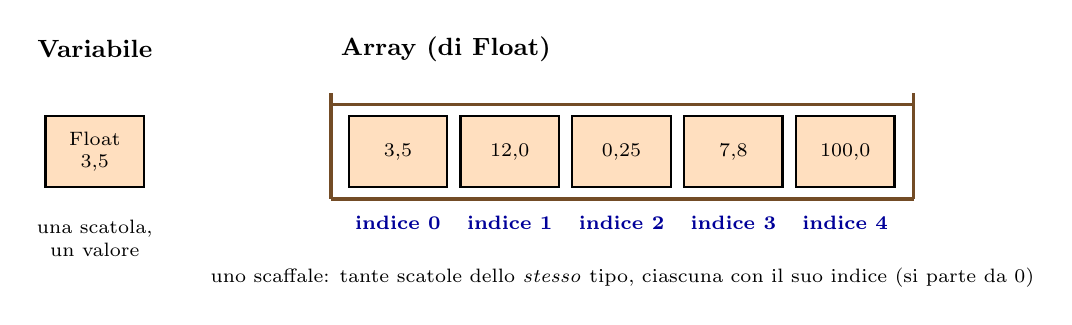
\begin{tikzpicture}[font=\footnotesize,
  ue7box/.style={draw, thick, fill=orange!25, minimum width=1.25cm, minimum height=0.9cm,
                 align=center, font=\scriptsize},
  ue7shelf/.style={draw, very thick, brown!60!black}]
  % variabile singola
  \node[font=\small\bfseries] at (0,2.3) {Variabile};
  \node[ue7box] (v) at (0,1.0) {Float\\3,5};
  \node[font=\scriptsize, align=center] at (0,-0.1) {una scatola,\\un valore};
  % array
  \begin{scope}[xshift=3.0cm]
    \node[font=\small\bfseries, anchor=west] at (0,2.3) {Array (di Float)};
    \draw[ue7shelf] (0,0.4) -- (7.4,0.4);
    \draw[ue7shelf] (0,1.6) -- (7.4,1.6);
    \draw[ue7shelf] (0,0.4) -- (0,1.75);
    \draw[ue7shelf] (7.4,0.4) -- (7.4,1.75);
    \node[ue7box] at (0.85,1.0) {3,5};
    \node[ue7box] at (2.27,1.0) {12,0};
    \node[ue7box] at (3.69,1.0) {0,25};
    \node[ue7box] at (5.11,1.0) {7,8};
    \node[ue7box] at (6.53,1.0) {100,0};
    \foreach \x/\i in {0.85/0, 2.27/1, 3.69/2, 5.11/3, 6.53/4} {
      \node[font=\scriptsize\bfseries, text=blue!60!black] at (\x,0.1) {indice \i};
    }
    \node[font=\scriptsize, align=center] at (3.7,-0.6) {uno scaffale: tante scatole
      dello \emph{stesso} tipo, ciascuna con il suo indice (si parte da 0)};
  \end{scope}
\end{tikzpicture}
\caption{La metafora del docente. Una variabile è una scatola che contiene un valore; un
array è uno scaffale che contiene tante scatole dello stesso tipo. Ogni posto dello
scaffale ha un indice, e il primo indice è 0. Schema ricostruito.}
\label{ue7:fig:scaffale}
\end{figure}

\paragraph{Approfondimento: array, set e map.} Romero e Sewell (capitolo 13, ``Data
Structures and Flow Control'') chiamano \textbf{contenitori} (\emph{containers}) le
strutture che raccolgono più valori dello stesso tipo, e nei Blueprint ce ne sono tre.
L'\textbf{array} è una lista ordinata con accesso per \textbf{indice}, ``e gli array
partono sempre dall'indice 0'': con quattro elementi, il primo ha indice 0 e l'ultimo
indice 3, cioè \emph{Length}~$-$~1. Il \textbf{set} è un insieme senza ordine e senza
doppioni, in cui si cerca per valore; la \textbf{map} associa a ogni \emph{chiave} un
\emph{valore} (per esempio il nome di un'arma e le sue munizioni). Sugli array si lavora
con una manciata di nodi: \textbf{Get (a copy)} legge l'elemento a un indice,
\textbf{Set Array Elem} lo modifica, \textbf{Add} aggiunge in fondo, \textbf{Insert}
inserisce a un indice spostando gli altri, \textbf{Length} e \textbf{Last Index} dicono
quanto è lungo, \textbf{Random Array Item} pesca un elemento a caso. Gli autori
avvertono: mai leggere un indice oltre l'ultimo, perché i risultati sono imprevedibili.
La tabella~\ref{ue7:tab:contenitori} riassume i quattro modi in cui una variabile può
essere costituita.

% ---------------------------------------------------------------------
\section{L'ereditarietà: parent e child}
\label{ue7:sec:ereditarieta}

La slide successiva riprende rapidamente le collisioni (``ripasseremo anche un po' le
collisioni'') e introduce il secondo concetto della giornata. ``Qualcuno di voi ha mai
sentito parlare dei concetti di \textbf{parent} e \textbf{child} in programmazione?''

\paragraph{Padre e figlio.} ``Mettiamo un esempio che possiamo vedere nella vita di tutti
i giorni'': il rapporto fra genitori e figli. ``Io, come figlio di mio padre, ho preso
una parte dei geni di mio padre'' (e di mia madre), ``e però, come essere unico, posso
variare nelle mie particolarità: non sono uguale, ma condivido comunque delle cose''.
Lo stesso succede con gli oggetti: ``ci sono degli oggetti che possono essere figli di
altri oggetti''. Esempio: un cubo \emph{parent} che nel Begin Play stampa un valore, e
fa solo quello. ``Il child mi stamperà sempre quel valore, ma magari stampa anche un
altro valore'': ``prende la caratteristica del papà, ma volendo può aggiungere, o
addirittura \textbf{sovrascrivere}, alcune azioni''.

\paragraph{Il cubo che diventa cilindro.} In Unreal i child si creano direttamente
dall'engine. In slide c'è il BP\_Cube delle lezioni precedenti: ``vogliamo farlo
diventare un cilindro? Creiamo un child e cambiamo semplicemente la Static Mesh''. ``Il
parent rimarrà un cubo, invece il figlio ha voluto cambiare forma'': per le
caratteristiche di Blueprint avranno lo stesso comportamento, ``oppure, volendo, lo
possiamo anche cambiare''. La figura~\ref{ue7:fig:gerarchia} mostra la gerarchia che si
costruirà oggi.

\begin{figure}[htbp]
\centering
\begin{tikzpicture}[font=\footnotesize,
  ue7cls/.style={draw, thick, rounded corners=4pt, align=center, fill=gray!8,
                 text width=3.3cm, minimum height=1.0cm, inner sep=4pt},
  ue7inh/.style={-{Triangle[open, length=3mm, width=3mm]}, thick}]
  \node[ue7cls, fill=gray!20] (actor) at (0,3.0) {\textbf{Actor}\\(classe di Unreal)};
  \node[ue7cls, fill=blue!10] (act) at (0,1.0) {\textbf{BP\_Activable}\\eventi
    Activation e Deactivation (Print String)};
  \node[ue7cls, fill=yellow!25] (light) at (-4.4,-1.4) {\textbf{BP\_ActivableLight}\\Point
    Light; override: accende e spegne};
  \node[ue7cls, fill=green!12] (ball) at (0,-1.4) {\textbf{BP\_BallMoving}\\(esercizio)
    override: Play e Reverse};
  \node[ue7cls, fill=orange!15] (plat) at (4.4,-1.4) {\textbf{piattaforma
    attivabile}\\(esercizio e compito)};
  \node[ue7cls, fill=gray!8] (btn) at (5.2,3.0) {\textbf{BP\_Button}\\array
    ActivableItems di tipo BP\_Activable};
  \draw[ue7inh] (act) -- (actor);
  \draw[ue7inh] (light.north) -- ++(0,0.6) -| (act.south);
  \draw[ue7inh] (ball) -- (act);
  \draw[ue7inh] (plat.north) -- ++(0,0.6) -| (act.south);
  \draw[ue7inh] (btn) -- (actor);
  \draw[-{Stealth[length=2.2mm]}, thick, dashed, violet!60!black] (btn.south) to[bend
    left=10] node[pos=0.45, right, font=\scriptsize, align=left]{contiene referenze\\a
    qualunque child} (act.east);
\end{tikzpicture}
\caption{La gerarchia di classi costruita nella lezione. Le frecce con la punta vuota
vanno dal child al parent (``eredita da''). BP\_Activable definisce i due eventi comuni;
ogni child li ridefinisce a modo suo. BP\_Button tiene un array di referenze di tipo
BP\_Activable, e quindi può contenere qualunque child. I nomi dei Blueprint
dell'esercizio sono quelli suggeriti dal docente; schema ricostruito.}
\label{ue7:fig:gerarchia}
\end{figure}

\paragraph{Approfondimento: superclasse, sottoclasse e tipo.} Romero e Sewell (capitolo
3, ``Object-Oriented Programming and the Gameplay Framework'') danno la versione
tecnica. Quando si crea un Blueprint, la prima cosa che si sceglie è la sua
\textbf{classe parent} (la \emph{superclasse}); un Blueprint ha \emph{un solo} parent,
ma può avere molti child (\emph{sottoclassi}). Il loro esempio sono le armi: una classe
base \emph{Weapon} con tutto ciò che è comune, e le armi concrete come figlie. Il
vantaggio è doppio. Da un lato, una funzione definita nel parent (\emph{Fire}) può
essere \textbf{ridefinita} (\emph{override}) in ogni child (il fucile a energia spara un
raggio, il lanciarazzi un razzo), e a runtime viene eseguita la versione della classe
effettiva dell'oggetto. Dall'altro, un child \textbf{è anche} del tipo del parent:
un'istanza del lanciarazzi è un \emph{Weapon}, e una variabile o un parametro di tipo
Weapon può contenerla. È esattamente il trucco su cui si regge il pulsante di oggi: una
variabile di tipo \emph{BP\_Activable} potrà contenere una luce, una piattaforma, una
palla, qualunque child degli attivabili. Del resto, ogni Blueprint della lezione è già un
child: BP\_Button ha come parent la classe \emph{Actor}.

% ---------------------------------------------------------------------
\section{La dimostrazione: il pulsante finito}
\label{ue7:sec:demo}

``Andremo a creare un bellissimo pulsantone. Eccolo qua.'' Nella scena del docente c'è
il risultato finale. Il giocatore sale sulla pedana, la pedana si abbassa e
\textbf{accende una luce} (``vedremo anche un pochino di \emph{lighting}''); se scende,
la luce si spegne. Nella stessa scena c'è una piattaforma che reagisce allo stesso
pulsante: ``ho creato una piattaforma di tipologia \textbf{attivabile}'', e luce e
piattaforma ``condividono'' qualcosa, ``sono della stessa classe, ma comportamenti
diversi''. Collegata la piattaforma al pulsante, la pressione accende la luce
\emph{e} manda giù la piattaforma; ``in questo caso ho fatto sì che andasse solo giù'':
quando la piattaforma è in basso ci si sale sopra, e lei torna su; si torna sul
pulsante, e di nuovo giù.

\paragraph{La domanda sull'interazione.} ``Faremo anche le interazioni, tipo premi E per
interagire?'' Sì: la prossima lezione sarà sulle \textbf{animazioni}, con un personaggio
animato, e l'interazione si farà con il \textbf{trace}, ``infatti il trace è collegato
al fatto dell'interazione'': ha interagito o non ha interagito.

\paragraph{Approfondimento: overlap o tasto?} I due modi di attivare qualcosa hanno usi
diversi. L'\emph{overlap} di un volume, quello di oggi, è passivo: scatta perché il
giocatore \emph{è} in un posto (pedane a pressione, trappole, cutscene). L'interazione
con un tasto è attiva: il giocatore guarda un oggetto e preme. Lo schema tipico, che la
lezione annuncia, è un \emph{line trace} dalla telecamera in avanti, eseguito alla
pressione del tasto; se colpisce un actor che ``sa'' interagire, gli si chiama un evento.
Per chiamarlo senza sapere in anticipo che classe abbia l'oggetto colpito si usa di
solito una \textbf{Blueprint Interface} (Romero e Sewell, capitolo 16): una lista di
funzioni senza corpo, che ogni classe interessata implementa a modo suo. È una cugina
dell'ereditarietà vista oggi, utile quando le classi da accomunare non hanno un parent
comune.

% ---------------------------------------------------------------------
\section{Il pulsante: due mesh e una box}
\label{ue7:sec:bottone}

``Allora, ragazzi, vi chiedo se siete pronti con il vostro progettino.'' Prima di
cominciare, la raccomandazione di sempre: tenere il progetto ordinato in
\textbf{cartelle}, ``perché se no un giorno succederà che non ritroverete'' le cose,
``come perdere qualcuno in un centro commerciale il sabato''. Nella cartella
\emph{Blueprint}, ``siamo al solito'': Blueprint Class, Actor. Il docente lo chiama
\textbf{BP\_Button1} (``io farò sempre il mio bellissimo BP\_Button1''); nel capitolo è
BP\_Button.

\paragraph{Due Static Mesh, non una.} ``Il bottone, per come sono fatte le mesh, sono due
Static Mesh'': una è il \textbf{frame}, la cornice, e l'altra la \textbf{piastra} che si
abbassa. Il docente le crea con Ctrl+C e Ctrl+V da un componente Static Mesh, e le
rinomina \textbf{Frame} e \textbf{Platform}; nel campo \emph{Static Mesh} assegna alla
prima la mesh della cornice della pedana a pressione (``se non sbaglio \emph{pressure
plate frame}'') e alla seconda quella della piastra (``\emph{pressure plate}\ldots{}
platform''); i nomi esatti degli asset nel progetto del corso non sono sicuri dalla
trascrizione. ``Essendo che sono fatti all'unisono'', i due pezzi sono già allineati.

\paragraph{Un consiglio per i 3D artist.} Il motivo della divisione vale per chiunque
modelli, o faccia modellare, oggetti interattivi. ``Se dovete fare un pulsante, non fate
fare un pulsante unico: fate fare un pulsante che è diviso'' fra la cornice (``quello che
sta attorno'') e la \emph{pressure plate}. ``Perché se adesso andiamo ad abbassare, ed è
un unico asset, tutto il bottone va giù, anche il frame, quindi si va a compenetrare col
pavimento.'' La regola: ``se ci sono delle cose interagibili a livello di movimentazione,
sappiate che è meglio sempre \textbf{splittarle}''. Poi, certo, ``dipende dalla
creatività'' e dal designer.

\paragraph{La box.} Terzo componente, ``la mitica'' \textbf{Box Collision}, scalata
perché sia ``leggermente unanime'' con il bottone, cioè della sua stessa impronta, e
alzata sull'asse Z: ``ricordatevi, attenzione a sotto''. E soprattutto, come per la
piattaforma della volta scorsa, \textbf{figlia della Platform}: ``la box deve seguire la
platform. Importante, in modo tale che se io sposto, si sposta con essa''
(figura~\ref{ue7:fig:bottone}).

\paragraph{È la box a comandare.} Una studentessa chiede conferma: ``bisogna fare la box
sopra perché è la box che interagisce, giusto?'' Sì: il player entra con i piedi nella
box, la box interagisce, la timeline parte e il pulsante va giù. ``Non è tanto la
piattaforma o il pulsante a triggerare l'evento, ma la box sopra.'' E perché non usare
l'overlap della mesh stessa? ``Perché le collisioni sono \textbf{troppo precise}'': sono
``a contatto con una superficie'', ``un controllo sempre più micro'', ``forse sì, forse
no'', e ``la possibilità di errore è molto più ampia''. Un volume, invece, dà una
risposta macro: ``sì, no''.

\begin{figure}[htbp]
\centering
\begin{tikzpicture}[font=\footnotesize,
  ue7comp/.style={draw, thick, rounded corners=3pt, align=left, fill=gray!8,
                  minimum height=0.6cm, text width=3.4cm, inner sep=4pt},
  ue7tree/.style={thick, gray!70!black}]
  \node[font=\small\bfseries, anchor=west] at (-0.2,1.0) {Components di BP\_Button};
  \node[ue7comp, anchor=west] (root) at (0,0.2) {DefaultSceneRoot};
  \node[ue7comp, anchor=west, fill=gray!20] (fr) at (0.6,-0.6) {\textbf{Frame}
    (Static Mesh)};
  \node[ue7comp, anchor=west, fill=blue!10] (pl) at (0.6,-1.4) {\textbf{Platform}
    (Static Mesh)};
  \node[ue7comp, anchor=west, fill=green!12] (bx) at (1.2,-2.2) {\textbf{Box} (Box
    Collision)};
  \node[ue7comp, anchor=west, fill=red!10] (tl) at (0,-3.0) {\textbf{PushButton}
    (Timeline)};
  \draw[ue7tree] (0.2,-0.1) |- (fr.west);
  \draw[ue7tree] (0.2,-0.1) |- (pl.west);
  \draw[ue7tree] (0.8,-1.7) |- (bx.west);
  % vista laterale
  \begin{scope}[xshift=7.4cm, yshift=-1.3cm]
    \draw[thick, gray] (-1.2,-1.0) -- (4.4,-1.0);
    \node[font=\scriptsize, gray] at (3.9,-1.25) {pavimento};
    \fill[gray!45, draw=black, thick] (-0.1,-1.0) rectangle (3.1,-0.75);
    \node[font=\scriptsize] at (1.5,-1.25) {Frame};
    \fill[blue!25, draw=blue!50!black, thick] (0.2,-0.75) rectangle (2.8,-0.5);
    \draw[thick, dashed, blue!50!black] (0.2,-0.85) rectangle (2.8,-0.6);
    \node[font=\scriptsize, anchor=west] at (3.2,-0.55) {Platform};
    \draw[-{Stealth[length=1.6mm]}, thick, red!60!black] (1.5,-0.45) -- (1.5,-0.72);
    \node[font=\scriptsize, red!60!black, anchor=west] at (1.6,-0.25) {$-10$ su Z};
    \draw[thick, dashed, green!50!black, fill=green!8, fill opacity=0.6]
      (0.3,-0.5) rectangle (2.7,0.15);
    \node[font=\scriptsize, green!40!black] at (1.0,-0.17) {Box};
    % omino
    \draw[thick] (-0.7,0.35) circle (0.13);
    \draw[thick] (-0.7,0.22) -- (-0.7,-0.35);
    \draw[thick] (-0.7,-0.35) -- (-0.85,-1.0);
    \draw[thick] (-0.7,-0.35) -- (-0.55,-1.0);
    \node[font=\scriptsize] at (-0.7,0.7) {player};
  \end{scope}
\end{tikzpicture}
\caption{I componenti del pulsante. A sinistra la gerarchia: Frame e Platform sono due
Static Mesh separate; la Box Collision è figlia della Platform, così la segue; la
timeline PushButton compare tra i componenti. A destra la vista laterale: la piastra
scende di 10 unità dentro la cornice (tratteggio), mentre la cornice resta ferma.
Schema ricostruito; le proporzioni non sono quelle dell'asset.}
\label{ue7:fig:bottone}
\end{figure}

% ---------------------------------------------------------------------
\section{Le collisioni della Static Mesh: simple e complex}
\label{ue7:sec:collisioni}

``Poi, se non sbaglio, su questo asset c'è un problema.'' È quello sollevato a inizio
lezione: il pulsante, come la piattaforma, potrebbe avere ``una collisione un po' tanto
alta'' per il personaggio.

\paragraph{Il Max Step Height.} Nel personaggio del giocatore c'è una variabile,
\textbf{Max Step Height}, ``che non ci permette di andare sopra queste tipologie di
asset'' se sono più alte di un certo valore. Il docente prova sulla sua scena: a lui va
``benissimo'', ``perché guardate cosa ho fatto io per ovviare a questo problema''. A
qualcuno degli studenti il personaggio si blocca con i piedi? Pare di no, ``bene''; ma
``per accortezza'', visto che al docente è capitato, si sistema la collisione della mesh.

\paragraph{Approfondimento: Max Step Height e Walkable Floor.} I due parametri stanno nel
\emph{Character Movement Component} del personaggio. Il \textbf{Max Step Height}
(predefinito 45 unità, cioè 45 centimetri) è l'altezza massima di uno ``scalino'' che il
personaggio può salire camminando, senza saltare; il \textbf{Walkable Floor Angle}
(predefinito 44,765 gradi) è la pendenza massima su cui può camminare. Se il bordo della
collisione di un oggetto supera lo scalino, la capsula del personaggio ci sbatte contro
come contro un muro. Si può alzare lo scalino del personaggio, ma cambia il modo in cui
si muove ovunque; di solito conviene sistemare la collisione dell'oggetto, come fa la
lezione.

\paragraph{L'editor della Static Mesh.} Si seleziona la mesh della piastra e si clicca
sulla ``finestrella blu'', l'icona dell'asset nel campo Static Mesh, per aprire
l'\textbf{editor della Static Mesh}: ``la schermata in cui Unreal fa vedere tutte le
particolarità delle collisioni dell'asset stesso'', ``dati molto più \emph{insight} del
modello''.

\paragraph{Una parentesi sui LOD.} Fra i dati ci sono i \textbf{LOD}, i \emph{level of
detail}: ``quella pratica di abbassare la risoluzione degli asset quando sono distanti,
in modo tale da avere ottimizzazione''. ``Sono tipo a 200 metri da me? Abbassa la
qualità, perché pesa.'' Il corso non li userà, ma è bene sapere che esistono.

\paragraph{Simple e complex.} Dal menù \textbf{Show} in alto si visualizzano le
collisioni dell'asset, e ``ci sono due tipologie di collisioni''.
\begin{itemize}
  \item Le \textbf{simple}, in \textbf{verde}: forme semplici, ``usate per avere
        interazioni di base''. Sono quelle che Unreal usa normalmente quando si mette un
        asset nella viewport, ``per tempi e cose di ottimizzazione''.
  \item Le \textbf{complex}, ``questi lineamenti blu'' (azzurri): la forma esatta del
        modello, triangolo per triangolo. Servono quando ``ci serve l'esatto punto''
        in cui si tocca l'oggetto. Esempio: un \textbf{sistema di scalata}, in cui
        ``devo andare a vedere il punto esatto in cui ho messo la mano'' per tirare su il
        personaggio (``poi ci sono anche alternative'').
\end{itemize}
Le due collisioni si preparano ``durante la modellazione'', e chi segue il corso di 3D
art le vedrà. Ma attenzione: ``se mettete le complex collision su tutti gli asset,
probabilmente potete dire ciao al vostro bellissimo PC'', a meno di ottimizzazioni
parallele. Qui servono le simple.

\paragraph{Modificare la collisione.} La cosa bella è che le collisioni simple si
possono modificare a mano. Cliccando sul ``reticoletto verde'' si possono muovere,
ruotare e scalare come un oggetto qualsiasi. Gli studenti dovrebbero avere una
collisione ``un po' più arzigogolata'', ``con tutti i reticolini''; il docente ha già
modificato la sua. La procedura:
\begin{enumerate}
  \item \textbf{cancellare} la collisione simple esistente, ``quella verde, non quella
        azzurra'';
  \item dal menù \textbf{Collision} aggiungerne una nuova, scegliendo fra
        \textbf{Sphere}, \textbf{Capsule}, \textbf{Box} e le varie \textbf{k-DOP} (10DOP-X,
        Y, Z, 18DOP, 26DOP; nella trascrizione ``10 di OP meno X'');
  \item per il pulsante, \textbf{Box} (``Box Simplified Collision''): ``a noi ci serve
        una scatoletta, è un quadrato alla fine'';
  \item selezionare la box e \textbf{stringerla} ``proprio un'anticchia'', abbassandola,
        dopo aver tolto lo \emph{snap}, ``quasi come se fosse una collisione già
        abbassata''.
\end{enumerate}
Ora il pulsante ``ha una collisione un po' più affondabile''.

\paragraph{Le forme a confronto.} Il docente prova le alternative una per una. La
\textbf{sfera} su una piastra quadrata ``non ci serve assolutamente, perché non è
coerente alla sua forma''. Le \textbf{k-DOP} invece seguono il modello con un numero
crescente di piani: ``sono il livello di dettaglio che la collisione avrà, il livello di
vertici''; ``più vertici ci sono, più le collisioni sono precise, meno spigolose''. Sul
cubetto la 10DOP sulla X, sulla Y e sulla Z danno risultati quasi uguali, con ``piccole
differenze'' di taglio; la 18DOP ``ha fatto gli angoli più precisi''; la 26DOP, ``il
massimo'', taglia anche gli spigoli (figura~\ref{ue7:fig:kdop}).

\paragraph{Un'esperienza di lavoro.} ``A me è capitato con un lavoro che ho fatto.'' Nel
livello c'era una piccola pista, e alcuni asset avevano collisioni ``estremamente
complesse'': il docente e il gruppo di designer hanno dovuto \textbf{cancellare tutte le
collisioni e rifarle} a mano, ``con i cubettini'', per semplificare il lavoro
dell'engine. La morale: le collisioni sono parte del lavoro del level designer, non solo
del modellatore.

\begin{figure}[htbp]
\centering
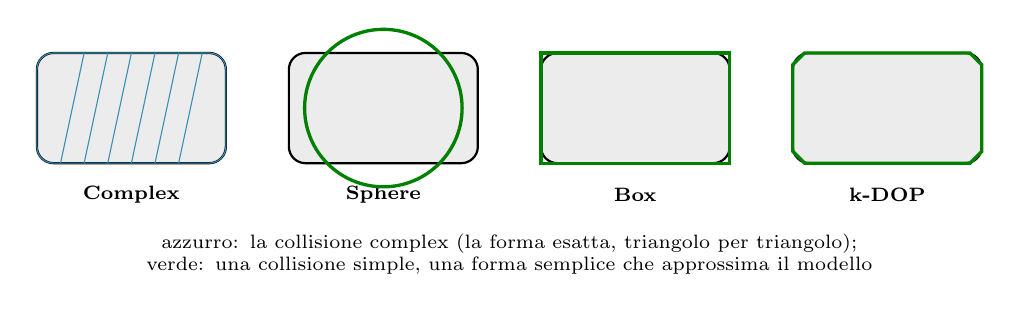
\begin{tikzpicture}[font=\footnotesize,
  ue7mesh/.style={draw=black, thick, fill=gray!15},
  ue7coll/.style={draw=green!50!black, very thick},
  ue7cplx/.style={draw=cyan!70!black, thin}]
  % modello: piastra con bordi smussati (vista dall'alto, stilizzata)
  \foreach \x/\nome in {0/Complex, 3.2/Sphere, 6.4/Box, 9.6/k-DOP} {
    \begin{scope}[xshift=\x cm]
      \draw[ue7mesh, rounded corners=6pt] (0,0) rectangle (2.4,1.4);
      \node[font=\scriptsize\bfseries] at (1.2,-0.4) {\nome};
    \end{scope}
  }
  % complex: segue tutto
  \draw[ue7cplx, rounded corners=6pt] (0,0) rectangle (2.4,1.4);
  \foreach \i in {0.3,0.6,...,2.1} {\draw[ue7cplx] (\i,0) -- (\i+0.3,1.4);}
  % sphere
  \draw[ue7coll] (4.4,0.7) circle (1.0);
  % box
  \draw[ue7coll] (6.4,0) rectangle (8.8,1.4);
  % kdop: ottagono
  \draw[ue7coll] (9.75,0) -- (11.85,0) -- (12.0,0.15) -- (12.0,1.25) -- (11.85,1.4)
    -- (9.75,1.4) -- (9.6,1.25) -- (9.6,0.15) -- cycle;
  \node[font=\scriptsize, align=center, text width=12cm] at (6.0,-1.15) {azzurro: la
    collisione complex (la forma esatta, triangolo per triangolo); verde: una collisione
    simple, una forma semplice che approssima il modello};
\end{tikzpicture}
\caption{Collisioni della piastra viste dall'alto, in forma stilizzata. La complex
segue ogni triangolo del modello; la Sphere non è coerente con la forma; la Box è la
scelta della lezione; le k-DOP aggiungono piani e smussano gli spigoli. Schema
ricostruito, non una schermata dell'editor.}
\label{ue7:fig:kdop}
\end{figure}

\paragraph{Approfondimento: Collision Complexity.} Nell'editor della Static Mesh, fra
i dettagli dell'asset, c'è l'impostazione \textbf{Collision Complexity}. Con il
valore predefinito (\emph{Project Default}, in pratica ``simple e complex separate'') le
query fisiche e il movimento dei personaggi usano la collisione simple, mentre i trace
che lo chiedono esplicitamente (il flag \emph{Trace Complex}) usano quella complex. Con
\emph{Use Complex Collision As Simple} la forma esatta viene usata per tutto: comodo per
un pavimento irregolare statico, ma costoso, e incompatibile con la simulazione fisica
dell'oggetto. Le k-DOP (\emph{discrete oriented polytope}) sono poliedri convessi che
racchiudono la mesh con 10, 18 o 26 piani a orientamento fisso; il menù
\emph{Collision} offre anche \emph{Auto Convex Collision}, che scompone la mesh in più
pezzi convessi, una via di mezzo fra la precisione della complex e il costo della
simple.

% ---------------------------------------------------------------------
\section{La timeline del pulsante}
\label{ue7:sec:timeline}

``Fatto questo, ritorniamo sul nostro bellissimo button e andiamo effettivamente a creare
quello che sarà il funzionamento di base'': il tasto si deve abbassare sulla Z.

\paragraph{Gli eventi e il controllo sul player.} ``Quello che abbiamo visto l'altra
volta'': con la Box selezionata, nella sezione degli eventi in fondo ai dettagli, si
creano \textbf{On Component Begin Overlap} e \textbf{On Component End Overlap}, ``tutti e
due''. Poi ``la solita cosa'': si verifica che sia il player, ``con Is Valid o con il
tag, ma noi facciamo più semplice''. Dall'\textbf{Other Actor} si tira fuori un
\textbf{==} (``uguale uguale'') con \textbf{Get Player Pawn}, e il risultato va in un
\textbf{Branch}.

\paragraph{La timeline.} Dal ramo True, ``abbiamo già detto che è una timeline quella
che useremo'': una nuova timeline, rinominata \textbf{PushButton}, avviata con
\textbf{Play from Start} (la differenza con Play si chiarirà nella
sezione~\ref{ue7:sec:play}). Quanto deve scendere il pulsante? Il docente lo misura
nella viewport: seleziona la piastra, attiva lo \emph{snap} (``molto meglio''), con passo
10, e la abbassa finché è ``totalmente abbassata''. Bastano \textbf{10 unità}: ``quindi
abbiamo capito che dovremmo abbassarla di 10''.

\paragraph{La curva.} Doppio clic sulla timeline. ``Il valore da mettere per la
lunghezza della timeline è \textbf{0,25 secondi}. È molto corto.'' Poi:
\begin{enumerate}
  \item una \textbf{float track};
  \item un punto (Shift e clic) a \textbf{tempo 0, valore 0};
  \item un secondo punto a \textbf{tempo 0,25} (``il massimo della nostra timeline'') e
        \textbf{valore $-$10}: ``farà un passaggio in 0,25 secondi da 0 a $-$10'';
  \item i due pulsantini \textbf{Zoom to Fit Horizontal} e \textbf{Zoom to Fit
        Vertical} (``le due freccine''), che adattano il grafico alla lunghezza e
        all'altezza della curva.
\end{enumerate}
Una domanda dalla chat (``come si chiama il pallino sulla timeline?'') riceve la risposta
già nota: Shift e clic. Rispetto alla piattaforma della volta scorsa c'è una differenza
importante: allora la traccia andava da 0 a 1 ed era un \emph{alfa} da dare a un Lerp;
oggi la traccia contiene \emph{direttamente} lo spostamento, in unità del mondo.

\paragraph{Il nome della traccia.} ``Abbiamo la New Track 0'': la si rinomina cliccandoci
sopra con \textbf{F2}, \textbf{PushButtonZ} (``facciamo una Z maiuscola''). Il pin sul
nodo prende lo stesso nome; a una studentessa resta scritto \emph{New Track 0} anche
dopo la rinomina, e il docente la rassicura: ``è solo il nome che gli abbiamo dato'', il
funzionamento non cambia.

\paragraph{Il movimento.} Nell'Event Graph:
\begin{itemize}
  \item dal pin \textbf{PushButtonZ} si crea un \textbf{Make Vector}, collegando il
        valore alla \textbf{Z} (``l'asse che ci interessa''); X e Y restano a 0, ``tanto
        la X è zero e rimane zero'';
  \item si trascina la Platform nel grafo e se ne tira fuori \textbf{Set Relative
        Location}, con il vettore in \emph{New Location}. ``È relative perché è
        relativa alla sua transform'': lo zero è quello della piastra dentro il
        Blueprint, non lo zero del mondo;
  \item il nodo va collegato all'\textbf{Update} della timeline.
\end{itemize}
In Play, sulla pedana, ``non esplode, vedete che si abbassa''. Ma non si rialza più:
``è normale''. Manca il ritorno: dall'\textbf{End Overlap}, con lo stesso controllo sul
player, si collega l'ingresso \textbf{Reverse} della timeline. ``Premuto, torna su;
premuto, torna su.'' ``Eccolo che abbiamo creato il nostro movimento del pulsante, non
ancora la sua funzionalità'' (figura~\ref{ue7:fig:grafobottone}).

\begin{figure}[htbp]
\centering
\begin{tikzpicture}[font=\footnotesize,
  ue7node/.style={draw, thick, rounded corners=4pt, align=center, fill=gray!8,
                  minimum height=0.8cm, text width=2.0cm},
  ue7ev/.style={ue7node, fill=red!12},
  ue7exec/.style={-{Stealth[length=2.5mm]}, very thick, black!80},
  ue7data/.style={-{Stealth[length=2mm]}, thick, violet!60!black}]
  \node[ue7ev, text width=2.6cm] (bo) at (0,1.2) {\textbf{On Component Begin
    Overlap} (Box)};
  \node[ue7ev, text width=2.6cm] (eo) at (0,-1.2) {\textbf{On Component End
    Overlap} (Box)};
  \node[ue7node, text width=1.9cm] (eq1) at (3.3,2.6) {Other Actor \textbf{==} Get
    Player Pawn};
  \node[ue7node, text width=1.3cm] (br1) at (3.3,1.2) {\textbf{Branch}};
  \node[ue7node, text width=1.3cm] (br2) at (3.3,-1.2) {\textbf{Branch}};
  \node[ue7node, text width=1.9cm] (eq2) at (3.3,-2.6) {Other Actor \textbf{==} Get
    Player Pawn};
  \node[ue7node, fill=red!8, text width=2.4cm, minimum height=2.6cm] (tl) at (7.3,0)
    {\textbf{Timeline}\\PushButton\\[2pt]\scriptsize 0,25 s\\da 0 a $-$10};
  \node[ue7node, text width=1.6cm] (mv) at (10.6,-1.4) {\textbf{Make Vector}\\X 0, Y 0};
  \node[ue7node, text width=2.3cm] (set) at (13.1,0.8) {Platform $\rightarrow$
    \textbf{Set Relative Location}};
  \draw[ue7exec] (bo) -- (br1);
  \draw[ue7exec] (eo) -- (br2);
  \draw[ue7data] (eq1) -- (br1);
  \draw[ue7data] (eq2) -- (br2);
  \draw[ue7exec] (br1.east) -- node[above, font=\scriptsize]{True} ++(0.7,0) |-
    node[pos=0.78, above, font=\scriptsize]{Play from Start} ([yshift=0.8cm]tl.west);
  \draw[ue7exec] (br2.east) -- node[below, font=\scriptsize]{True} ++(0.7,0) |-
    node[pos=0.78, below, font=\scriptsize]{Reverse} ([yshift=-0.8cm]tl.west);
  \draw[ue7exec] ([yshift=0.8cm]tl.east) -- node[above, font=\scriptsize]{Update}
    (set.west);
  \draw[ue7data] ([yshift=-0.6cm]tl.east) -- node[above, font=\scriptsize, pos=0.5]{PushButtonZ}
    ++(0.6,0) |- (mv.west);
  \draw[ue7data] (mv.east) -| node[pos=0.3, below, font=\scriptsize]{Z $\rightarrow$
    New Location} (set.south);
\end{tikzpicture}
\caption{Il movimento del pulsante. Il Begin Overlap della Box, se l'actor è il player,
fa partire la timeline PushButton da capo; l'End Overlap la manda in Reverse. A ogni
Update il valore della traccia (da 0 a $-$10 in 0,25 secondi) diventa la Z di un
vettore, e la piastra si sposta con Set Relative Location. Schema ricostruito.}
\label{ue7:fig:grafobottone}
\end{figure}

\paragraph{Approfondimento: perché qui niente Lerp.} La sesta lezione aveva mostrato il
metodo ``giusto'' per la piattaforma: una traccia da 0 a 1 usata come alfa di un Lerp
fra due posizioni salvate. Qui il docente sceglie la strada diretta, e funziona per due
ragioni. La prima: il valore della traccia è \emph{assoluto}, non si somma alla posizione
corrente, quindi non si accumula (era il difetto del primo metodo della volta scorsa).
La seconda: la piastra è figlia di una radice ferma, e la sua posizione relativa di
partenza è (0, 0, 0), quindi ``$-$10 rispetto alla radice'' vuol dire esattamente ``10
più in basso di dove sta''. Se la piastra fosse stata spostata nel Blueprint, per
esempio a Z 5, il primo Update la teletrasporterebbe a Z 0: in quel caso serve sommare
lo spostamento alla posizione iniziale salvata, o tornare al Lerp. Per oggetti che si
spostano di poco, una traccia in unità del mondo è la soluzione più leggibile.

% ---------------------------------------------------------------------
\section{Le curve: linear e auto}
\label{ue7:sec:curve}

``Adesso vi faccio vedere anche una particolarità, che potremmo usare anche per la
piattaforma'': si può \textbf{modificare la tipologia dei punti}.

\paragraph{Lineari.} I punti creati finora sono \textbf{lineari}: ``formano una linea'',
e l'aumento o la diminuzione del valore ``è sempre costante'' nel tempo: in ogni
frazione di secondo il valore cambia sempre della stessa quantità, ``tra un punto e
l'altro''.

\paragraph{Curve.} ``Se invece vogliamo una curva un po' più \emph{smooth}'', si fa tasto
destro su un punto: compare la serie di \textbf{Key Interpolation}, ``cioè ti dice: quale
tipo di punto vuoi che sia?''. Il docente sceglie \textbf{Auto}, e la linea diventa una
curva; lo stesso sull'altro punto. Ora, con i ``piccoli braccetti'' (le tangenti) di
ciascun punto, si può modellare ``come nel tempo questa linea va da punto A a punto B''
(figura~\ref{ue7:fig:curve}, tabella~\ref{ue7:tab:interp}).

\paragraph{A che cosa serve.} Una studentessa chiede che cosa cambi in pratica. Il
docente prova: allunga la timeline a 1 secondo e piega la curva in modo che superi il
valore finale e poi ci ritorni. Il risultato, con un'escursione di appena 10 unità, sono
``micro movimenti'': il pulsante ``fa boom e ritorna su'', ``su e giù e si abbassa''.
``Cambiare la forma della curva ci permette di creare dei piccoli intervalli di vario
tipo'': il movimento rallenta, accelera, rimbalza. Su un pulsante si vede poco (``è molto
piccolo come spazio''); ``magari in pausa'' il docente propone di mostrarlo con ``una
piccola sferetta che fa su e giù''. Poi rimette la curva com'era.

\begin{figure}[htbp]
\centering
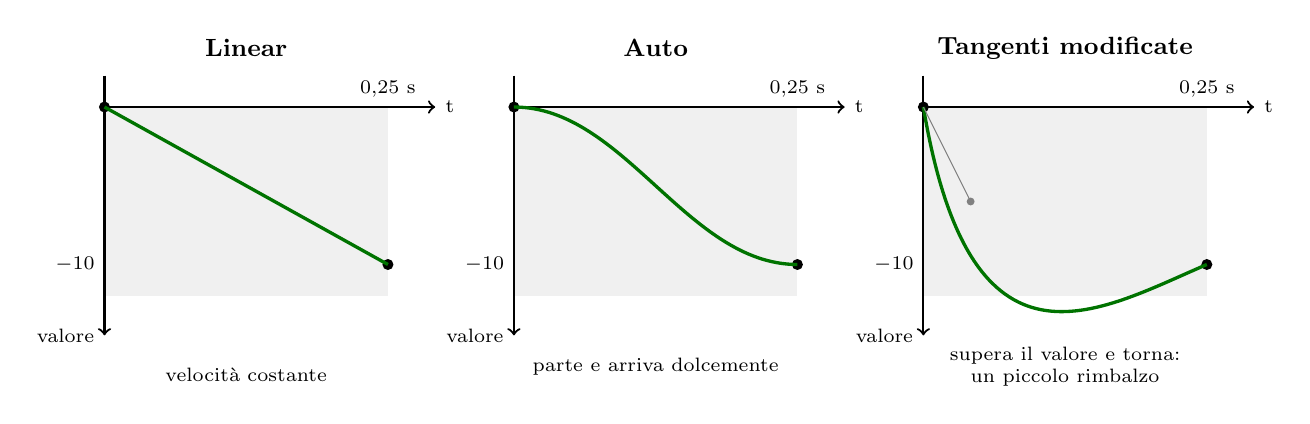
\begin{tikzpicture}[font=\footnotesize]
  \foreach \x/\titolo in {0/Linear, 5.2/Auto, 10.4/Tangenti modificate} {
    \begin{scope}[xshift=\x cm]
      \fill[gray!12] (0,-2.4) rectangle (3.6,0);
      \draw[->, thick] (0,0) -- (4.2,0) node[right, font=\scriptsize]{t};
      \draw[->, thick] (0,0.4) -- (0,-2.9) node[left, font=\scriptsize]{valore};
      \node[font=\scriptsize, left] at (0,-2.0) {$-10$};
      \node[font=\scriptsize, above] at (3.6,0) {0,25 s};
      \node[font=\small\bfseries] at (1.8,0.75) {\titolo};
      \fill (0,0) circle (0.07);
      \fill (3.6,-2.0) circle (0.07);
    \end{scope}
  }
  \draw[very thick, green!45!black] (0,0) -- (3.6,-2.0);
  \draw[very thick, green!45!black] (5.2,0) .. controls (6.6,0) and (7.4,-2.0) ..
    (8.8,-2.0);
  \draw[very thick, green!45!black] (10.4,0) .. controls (11.0,-3.6) and (12.6,-2.6) ..
    (14.0,-2.0);
  \draw[gray, thin] (10.4,0) -- (11.0,-1.2);
  \fill[gray] (11.0,-1.2) circle (0.05);
  \node[font=\scriptsize, align=center] at (1.8,-3.4) {velocità costante};
  \node[font=\scriptsize, align=center] at (7.0,-3.3) {parte e arriva dolcemente};
  \node[font=\scriptsize, align=center] at (12.2,-3.3) {supera il valore e torna:\\un
    piccolo rimbalzo};
\end{tikzpicture}
\caption{La stessa traccia con tre interpolazioni. Con le key lineari il pulsante scende
a velocità costante; con Auto la curva è morbida agli estremi; trascinando le tangenti
(i ``braccetti'') si ottengono andamenti come il rimbalzo provato a lezione. Schema
ricostruito.}
\label{ue7:fig:curve}
\end{figure}

\begin{table}[htbp]
\centering
\small
\begin{tabular}{@{}p{3.0cm}p{11.0cm}@{}}
\toprule
\textbf{Key Interpolation} & \textbf{Andamento fino alla key successiva} \\
\midrule
Auto & curva morbida, con tangenti calcolate in automatico (la scelta della lezione) \\
User & curva morbida con tangenti impostate a mano trascinando i ``braccetti'' \\
Break & come User, ma le due tangenti del punto si muovono in modo indipendente
(spigoli voluti) \\
Linear & retta: variazione costante nel tempo (il comportamento predefinito dei punti
creati con Shift e clic) \\
Constant & il valore resta fermo e salta alla key successiva al suo arrivo (a
gradino) \\
\bottomrule
\end{tabular}
\caption{I tipi di interpolazione di una key, dal menù del tasto destro su un punto della
timeline. La lezione usa Linear e Auto; le altre voci sono un'integrazione basata
sull'editor di Unreal Engine 5.}
\label{ue7:tab:interp}
\end{table}

\paragraph{Approfondimento: \emph{easing} e \emph{game feel}.} Le curve sono lo strumento
più economico per dare \emph{peso} a un movimento. In animazione si parla di
\emph{ease in} e \emph{ease out} (partire e arrivare lentamente) e di
\emph{overshoot} (superare la meta e tornare indietro, come il rimbalzo provato dal
docente): una porta che rallenta prima di chiudersi, un pulsante che affonda di colpo e
risale con un piccolo rimbalzo, un ascensore che parte dolcemente. A parità di durata,
un movimento lineare appare meccanico, uno con l'\emph{easing} appare fisico. Nelle
timeline la curva è anche un \emph{asset} riutilizzabile: dall'editor la traccia si può
salvare come \textbf{Curve Float} esterna e usare in più timeline, così tutti i pulsanti
del gioco si muovono allo stesso modo e si correggono in un punto solo.

% ---------------------------------------------------------------------
\section{I problemi degli studenti con il pulsante}
\label{ue7:sec:problemibottone}

``Il mio bottone non scende.'' ``Neanche a me.'' Il docente ripassa il grafo (Platform,
Set Relative Location sull'Update, il pin della traccia nella Z del Make Vector) e poi
chiama le studentesse in condivisione, una alla volta, ``Lucrezia per prima''. La
condivisione dello schermo su Zoom richiede diversi tentativi, fra permessi da dare,
barre degli strumenti che spariscono e un'eco ``quasi un boomerang''; alla fine
funziona.
\begin{itemize}
  \item \textbf{Il volume.} La box è ``molto piccola'' e il volume ``troppo basso'': deve
        stare sopra la piastra.
  \item \textbf{I punti della curva.} Il primo punto non sta a tempo 0: ``devi mettere
        tempo zero, valore zero''; il secondo a 0,25 e $-$10 ``va benissimo''. E le due
        freccine dello Zoom to Fit aiutano a vedere davvero la curva.
  \item \textbf{La lunghezza.} Un'altra studentessa ha messo 0,25 nel tempo del punto ma
        ha lasciato la \textbf{Length} della timeline al valore predefinito: ``devi
        modificare la lunghezza; vedi, c'è scritto \emph{Length} sopra''.
  \item \textbf{Stop invece di Reverse.} Sull'End Overlap era collegato \emph{Stop}: il
        pulsante si ferma dov'è invece di tornare su.
  \item \textbf{L'Update scollegato.} Il caso più istruttivo: il Set Relative Location
        aveva il pin dei dati collegato, ma non quello di \textbf{esecuzione}
        all'Update. ``Qui devi collegare solo l'execution pin.'' ``Ricordati, fai conto
        che l'Update è quello che fa'' il lavoro nel tempo della linea del tempo.
\end{itemize}
Un consiglio di contorno: ``spostati un po' gli asset'' di prova delle lezioni
precedenti, che potrebbero dare fastidio ai ``grubetti'' (forse i cubetti della
matrice).

\paragraph{Approfondimento: dati senza esecuzione.} L'ultimo errore è il più tipico di chi
viene da altri strumenti. Nei Blueprint i \textbf{pin di dati} (colorati) dicono
\emph{con che cosa} lavora un nodo, i \textbf{pin di esecuzione} (bianchi) dicono
\emph{quando} il nodo viene eseguito. Un nodo con i soli dati collegati non viene mai
eseguito: i suoi ingressi verrebbero calcolati se qualcuno lo chiamasse, ma nessuno lo
chiama. Fanno eccezione i nodi \emph{pure}, senza pin bianchi (come Make Vector o
Get Player Pawn), che vengono calcolati quando un nodo eseguito ne legge l'uscita. Il
controllo da fare quando ``non succede niente'' è quindi sempre lo stesso: seguire il
filo bianco dall'evento fino all'ultimo nodo.

% ---------------------------------------------------------------------
\section{Play o Play from Start?}
\label{ue7:sec:play}

``Posso fare una domanda rapidissima? Perché abbiamo usato Play from Start e non
Play?'' La risposta del docente, con un esempio di timeline da 0 a 2 secondi.
\begin{itemize}
  \item Con \textbf{Play}, se ci si ferma a 1 secondo (si esce dal pulsante quando la
        piastra ``sta a metà'') e poi si rientra, la timeline ``continuerà da quel punto
        in particolare dove ci siamo fermati'': da 1 a 2.
  \item Con \textbf{Play from Start}, se si esce e si rientra, la timeline ``riparte da
        0, non da 1''.
\end{itemize}
Nel caso del pulsante, dice il docente, ``non abbiamo particolari interruzioni, perché
abbiamo proprio un \emph{in} e \emph{out}''.

\paragraph{Approfondimento: che cosa succede davvero con il Reverse.} Con un pulsante
così breve la differenza si nota poco, ma esiste, ed è utile capirla con la
figura~\ref{ue7:fig:play}. Si entra, la timeline va avanti; si esce a metà, e il Reverse
la fa tornare indietro \emph{da dove si trova}. Se si rientra prima che sia tornata a 0:
\begin{itemize}
  \item con \textbf{Play} la timeline inverte di nuovo la direzione dal punto in cui è,
        e la piastra riprende a scendere senza scatti;
  \item con \textbf{Play from Start} la timeline salta a 0: la piastra torna di colpo in
        alto e riparte a scendere, un piccolo scatto visibile.
\end{itemize}
Per oggetti che vanno avanti e indietro seguendo un ingresso e un'uscita (pulsanti,
porte, piattaforme) la coppia più naturale è quindi \textbf{Play} e \textbf{Reverse}; è
proprio quella che il docente raccomanderà nell'esercizio finale
(sezione~\ref{ue7:sec:esercizio}) e che correggerà nella soluzione di uno studente
(``mettilo su Play, non Play from Start''). Play from Start serve quando ogni attivazione
deve ripetere l'animazione da capo, per esempio un colpo o un lampo.

\begin{figure}[htbp]
\centering
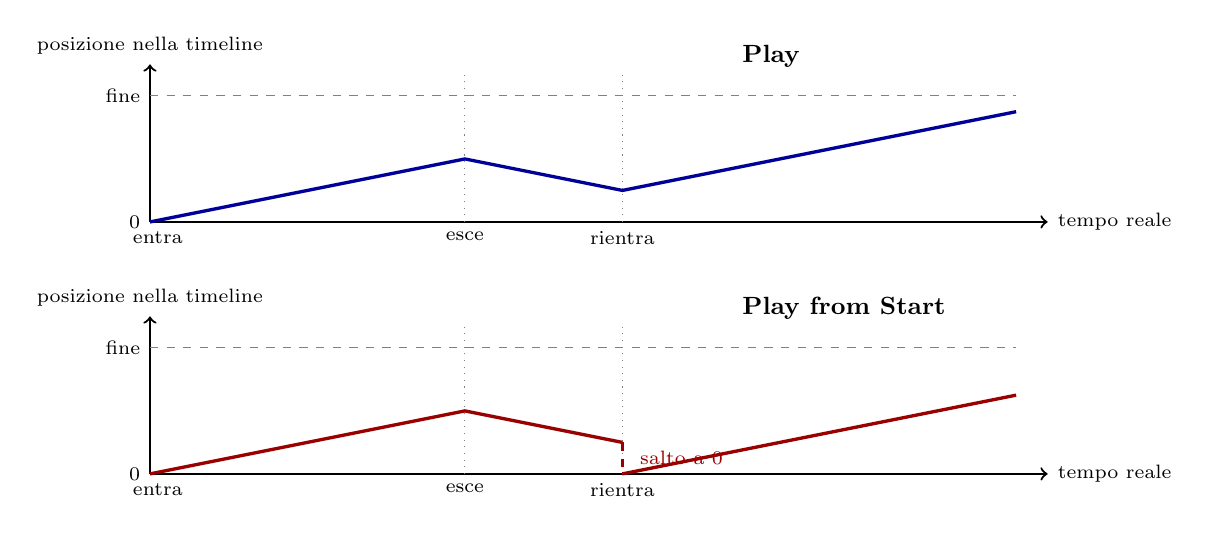
\begin{tikzpicture}[font=\footnotesize, x=1.0cm, y=1.0cm]
  \foreach \y/\titolo in {0/Play, -3.2/Play from Start} {
    \begin{scope}[yshift=\y cm]
      \draw[->, thick] (0,0) -- (11.4,0) node[right, font=\scriptsize]{tempo reale};
      \draw[->, thick] (0,0) -- (0,2.0) node[above, font=\scriptsize]{posizione nella
        timeline};
      \draw[gray, dashed] (0,1.6) -- (11,1.6);
      \node[font=\scriptsize, left] at (0,1.6) {fine};
      \node[font=\scriptsize, left] at (0,0) {0};
      \node[font=\small\bfseries, anchor=west] at (7.4,2.1) {\titolo};
      \draw[gray, dotted] (4,0) -- (4,1.9);
      \draw[gray, dotted] (6,0) -- (6,1.9);
      \node[font=\scriptsize, below] at (0.1,0) {entra};
      \node[font=\scriptsize, below] at (4,0) {esce};
      \node[font=\scriptsize, below] at (6,0) {rientra};
    \end{scope}
  }
  % Play
  \draw[very thick, blue!60!black] (0,0) -- (4,0.8) -- (6,0.4) -- (11,1.4);
  % Play from start
  \draw[very thick, red!60!black] (0,-3.2) -- (4,-2.4) -- (6,-2.8);
  \draw[very thick, red!60!black, dashed] (6,-2.8) -- (6,-3.2);
  \draw[very thick, red!60!black] (6,-3.2) -- (11,-2.2);
  \node[font=\scriptsize, red!60!black, anchor=west] at (6.1,-3.0) {salto a 0};
\end{tikzpicture}
\caption{Entrare, uscire a metà e rientrare prima che la timeline sia tornata a 0. Con
Play (in alto) la timeline riprende da dove si trova; con Play from Start (in basso)
salta all'inizio, e l'oggetto fa uno scatto. Schema ricostruito come integrazione alla
risposta del docente.}
\label{ue7:fig:play}
\end{figure}

% ---------------------------------------------------------------------
\section{Gli attivabili: la classe BP\_Activable}
\label{ue7:sec:activable}

``Adesso andiamo a fare una cosa bellina.'' Il pulsante si muove, ma non fa ancora
niente. Prima di creare la luce, ``prima, importante'', serve una \textbf{tipologia di
actor}: quella degli \textbf{attivabili}, ``quelli che per noi saranno gli attivabili''.

\paragraph{La classe base.} Un nuovo Blueprint Class di tipo Actor: il docente lo chiama
BP\_Activable1, qui è semplicemente \textbf{BP\_Activable}. ``Che succede qui all'interno? Ci serve solo
questo'': con la sola creazione ``abbiamo intanto definito una tipologia di actor''.
Dentro, due \textbf{Custom Event}:
\begin{itemize}
  \item \textbf{Activation}, collegato a un Print String ``attivato'';
  \item \textbf{Deactivation}, collegato a un Print String ``deattivato'' (cioè
        disattivato).
\end{itemize}
``Questi due eventi saranno collegati all'attivare qualcosa o disattivare qualcosa.'' Le
due stampe sono provvisorie: servono a vedere che il collegamento funziona, e poi a
capire come i figli possono \emph{sovrascrivere} gli eventi del padre
(sezione~\ref{ue7:sec:override}).

\paragraph{La domanda.} ``Quando è che io lo devo chiamare? E soprattutto, come faccio a
fargli dire: ehi, bottone, guarda che devi attivare questo esatto elemento?'' La risposta
è una variabile nel bottone, ed è il cuore della lezione.

% ---------------------------------------------------------------------
\section{Il bottone e la lista degli attivabili}
\label{ue7:sec:array}

\paragraph{Una variabile di tipo BP\_Activable.} Nel Blueprint del bottone si crea una
variabile, \textbf{ActivableItems}, e se ne cambia il tipo. ``Questo è molto
interessante, ragazzi: possiamo creare una variabile del tipo di quell'asset che abbiamo
appena creato'': il tipo è \textbf{BP\_Activable}, nella forma \emph{Object Reference}.
Una variabile così non contiene un numero o un testo, ma un \textbf{riferimento} a un
attivabile presente nel livello.

\paragraph{Pubblica.} ``Facciamola \textbf{pubblica}, e si fa con questo
\textbf{occhietto}'' accanto alla variabile. Il docente mette nel livello un
BP\_Activable e seleziona il pulsante: nei Details, in \emph{Default}, ``è apparso
Activable Items''. ``Vuol dire che questa variabile è modificabile dai Details del nostro
editor'', e quindi ``ci permette di avere interazioni dirette con la viewport,
l'ambiente di gioco'': ogni copia del pulsante nel livello può avere i suoi oggetti da
attivare.

\paragraph{Un array.} ``All'inizio di lezione abbiamo parlato degli array'': il pulsante
non deve attivare un oggetto solo, ``ma una moltitudine di oggetti''. Si cambia quindi
non la \emph{tipologia} della variabile, ma la sua \textbf{costituzione} (``cerchiamo di
dividerli'', precisa il docente): accanto al \emph{Variable Type} c'è un'icona (``questo
cilindro, vabbè, un'ellisse'') con una freccetta, e il menù offre \textbf{Single},
\textbf{Array}, \textbf{Set} e \textbf{Map} (tabella~\ref{ue7:tab:contenitori}). Si sceglie
Array, e l'icona della variabile cambia: ``diventa una matrice'', una griglia di
quadratini. ``Adesso abbiamo una variabile array di tipologia BP\_Activable.''

\begin{table}[htbp]
\centering
\small
\begin{tabular}{@{}p{2.4cm}p{5.8cm}p{5.8cm}@{}}
\toprule
\textbf{Costituzione} & \textbf{Che cosa contiene} & \textbf{Esempio} \\
\midrule
Single & un valore solo (la ``scatola'') & la referenza a una sola luce \\
Array & una lista ordinata di valori dello stesso tipo, con indice da 0; ammette
doppioni & gli oggetti attivati dal pulsante (ActivableItems) \\
Set & un insieme di valori unici, senza ordine e senza indice & i nomi degli oggetti
già raccolti \\
Map & coppie chiave--valore, con chiavi uniche & il nome di un'arma e le sue
munizioni \\
\bottomrule
\end{tabular}
\caption{Le quattro costituzioni di una variabile, dal menù accanto al Variable Type.
La lezione usa Single e Array; le descrizioni di Set e Map seguono Romero e Sewell
(capitolo 13).}
\label{ue7:tab:contenitori}
\end{table}

\paragraph{Quando chiamare gli attivabili.} ``Vogliamo che quando il nostro bel bottone
finisce di fare il suo percorso, e si schiaccia'', partano le attivazioni: si usa
l'uscita \textbf{Finished} della timeline. Ma Finished scatta sia alla fine della
discesa sia alla fine della risalita (dopo il Reverse), quindi bisogna sapere ``che
direzione è''. ``Vi ricordate che abbiamo usato lo Switch l'altra volta sulla
Direction?'' Dal pin \textbf{Direction} si crea uno \textbf{Switch on
ETimelineDirection}, collegato al Finished:
\begin{itemize}
  \item \textbf{Forward}: la timeline è andata avanti, il pulsante è schiacciato,
        quindi \textbf{attiva};
  \item \textbf{Backward}: la timeline è tornata indietro, il pulsante è tornato
        ``alla sua posizione di prima'', quindi \textbf{disattiva}.
\end{itemize}

\paragraph{Il For Each Loop.} ``Abbiamo già visto il For Loop. Questo è il \textbf{For
Each Loop}.'' Si prende un \emph{Get} di ActivableItems e se ne tira fuori il ciclo:
``questa esecuzione verrà fatta per ogni elemento dell'array che abbiamo inserito qua
dentro''; ``abbiamo cinque elementi dentro l'array, verrà fatto cinque volte''. Il nodo ha
due uscite di dati: l'\textbf{Array Element}, ``il singolo elemento che ha preso in
considerazione nel momento preciso del ciclo'', e l'\textbf{Array Index}. Dall'Array
Element, che è di tipo BP\_Activable, si può chiamare direttamente l'evento
\textbf{Activation}, collegato al \textbf{Loop Body}. Per il ramo Backward ``i primi due
li prendete, li copiate, li mettete sotto'': stesso Get, stesso For Each Loop, ma con
\textbf{Deactivation} (figura~\ref{ue7:fig:foreach}).

\begin{figure}[htbp]
\centering
\begin{tikzpicture}[font=\footnotesize,
  ue7node/.style={draw, thick, rounded corners=4pt, align=center, fill=gray!8,
                  minimum height=0.8cm, text width=2.0cm},
  ue7var/.style={ue7node, fill=blue!10, rounded corners=8pt},
  ue7ev/.style={ue7node, fill=red!12},
  ue7exec/.style={-{Stealth[length=2.5mm]}, very thick, black!80},
  ue7data/.style={-{Stealth[length=2mm]}, thick, violet!60!black}]
  \node[ue7node, fill=red!8, text width=1.8cm, minimum height=1.8cm] (tl) at (0,0)
    {\textbf{Timeline}\\PushButton};
  \node[ue7node, text width=2.1cm] (sw) at (3.3,0) {\textbf{Switch on
    ETimelineDirection}};
  \node[ue7node, text width=1.9cm] (fe1) at (6.7,1.4) {\textbf{For Each Loop}};
  \node[ue7node, text width=1.9cm] (fe2) at (6.7,-1.4) {\textbf{For Each Loop}};
  \node[ue7var, text width=2.4cm] (g1) at (6.7,3.1) {\textbf{Get}\\ActivableItems};
  \node[ue7var, text width=2.4cm] (g2) at (6.7,-3.1) {\textbf{Get}\\ActivableItems};
  \node[ue7ev, text width=2.1cm] (a) at (10.4,1.4) {Array Element $\rightarrow$
    \textbf{Activation}};
  \node[ue7ev, text width=2.1cm] (d) at (10.4,-1.4) {Array Element $\rightarrow$
    \textbf{Deactivation}};
  \draw[ue7exec] ([yshift=0.4cm]tl.east) -- node[above, font=\scriptsize]{Finished}
    ([yshift=0.4cm]sw.west);
  \draw[ue7data] ([yshift=-0.4cm]tl.east) -- node[below, font=\scriptsize]{Direction}
    ([yshift=-0.4cm]sw.west);
  \draw[ue7exec] (sw.north) |- node[pos=0.25, left, font=\scriptsize]{Forward} (fe1.west);
  \draw[ue7exec] (sw.south) |- node[pos=0.25, left, font=\scriptsize]{Backward} (fe2.west);
  \draw[ue7data] (g1) -- node[right, font=\scriptsize]{Array} (fe1);
  \draw[ue7data] (g2) -- node[right, font=\scriptsize]{Array} (fe2);
  \draw[ue7exec] (fe1) -- node[above, font=\scriptsize]{Loop Body} (a);
  \draw[ue7exec] (fe2) -- node[below, font=\scriptsize]{Loop Body} (d);
\end{tikzpicture}
\caption{Il pulsante chiama gli attivabili. Alla fine della timeline, lo Switch sulla
Direction sceglie il ramo: in avanti (pulsante schiacciato) un For Each Loop chiama
Activation su ogni elemento di ActivableItems; all'indietro (pulsante rilasciato) un
secondo ciclo chiama Deactivation. Schema ricostruito.}
\label{ue7:fig:foreach}
\end{figure}

\paragraph{Riempire l'array.} ``Ci manca ancora una piccola particolarità'': la variabile
è pubblica perché gli oggetti da attivare si scelgono \emph{nel livello}. Si clicca sul
pulsante nella scena, e in \emph{Default} c'è Activable Items: con il \textbf{+} si
aggiungono gli elementi, ``tutti quelli che volete''. Prima, però, un'avvertenza: ``in
informatica si parte non da uno, ma da \textbf{zero}''; ``l'indice 0 è il primo
indice''. Il primo elemento dell'array è l'elemento 0. Per assegnargli un oggetto ci sono
due modi:
\begin{itemize}
  \item il \textbf{menù a tendina}, che elenca ``tutti gli oggetti che puoi ficcarci
        dentro questo array'', cioè tutti i BP\_Activable presenti nel livello, ``perché
        giustamente è quello'';
  \item il \textbf{contagocce} (\emph{pick actor from scene}), ``proprio come su
        Photoshop'': si clicca sull'icona e si passa sopra gli oggetti della scena;
        sugli oggetti di un altro tipo l'editor avvisa che ``non è compatibile'', sul
        BP\_Activable invece ``è compatibile, ci può entrare dentro''. Un clic, ``ecco che
        è apparso''.
\end{itemize}
In Play, sul pulsante: ``attivato''; si scende: ``disattivato''. ``Vi funziona?''

\paragraph{I problemi.} A una studentessa, sul pulsante non compare la voce dell'array:
``basta che vai dove sono le variabili: c'è l'occhietto. Hai l'occhietto chiuso?''. Si
apre l'occhio, si compila (``se no non va''), e la voce compare. Poi bisogna
\textbf{mettere in scena} l'attivabile, se non c'è, e collegarlo con il contagocce
(``c'è la freccettina, c'è questo mouse con dei riquadri, e subito dopo c'è il
contagocce''). ``Sì, funziona. Ottimo.''

``Quindi, ragazzi, adesso abbiamo creato il funzionamento base'', cioè ``la relazione
tra pulsante e oggetto''. L'oggetto non ha ancora particolari funzionalità, ``se non
stampare due frasi'', ``tuttavia la base ce l'abbiamo''.

\paragraph{Approfondimento: la comunicazione diretta.} Quello costruito è ciò che Romero
e Sewell (capitolo 4) chiamano \textbf{Direct Blueprint Communication}: un Blueprint
tiene una variabile referenza a un altro actor, e la usa come \emph{Target} per
chiamarne le funzioni e gli eventi. Il loro esempio è sorprendentemente vicino a quello
della lezione: un \emph{BP\_LightSwitch} con una variabile di tipo Point Light, resa
\textbf{Instance Editable} (l'``occhietto'' del docente: ogni istanza nel livello può
avere un valore diverso), che a ogni overlap del giocatore accende o spegne una lampada
scelta nei Details dal menù a tendina. La lezione fa un passo in più in due direzioni:
la referenza è un \emph{array}, quindi un pulsante comanda molti oggetti; e il tipo è una
classe \emph{parent} scritta da noi, quindi il pulsante non sa e non deve sapere se
l'oggetto è una luce o una piattaforma. Il libro aggiunge un consiglio che vale anche
qui: prima di usare una referenza, controllarla con \textbf{Is Valid}, perché un elemento
dell'array lasciato vuoto nei Details (il \textbf{+} premuto senza scegliere niente)
produrrebbe l'errore ``Accessed None'' visto a inizio lezione. Lo stesso capitolo 13
mostra il For Each Loop proprio su un array di Point Light, ``le lampade di una
stanza''.

% ---------------------------------------------------------------------
\section{Il figlio: BP\_ActivableLight e i due Begin Play}
\label{ue7:sec:child}

``A questo punto andiamo a evolvere questo attivabile in una luce che si accende e si
spegne.'' Ma, attenzione: ``non andiamo a creare un nuovo Blueprint, ma andiamo a creare
un \textbf{figlio} di questo Blueprint, perché vogliamo che condivida la particolarità di
avere le fasi di attivazione e disattivazione''.

\paragraph{Create Child Blueprint Class.} Tasto destro su BP\_Activable nel Content
Browser, \textbf{Create Child Blueprint Class} (``lo trovate tutto sopra''). Unreal
propone un nome con il suffisso \emph{Child}; il docente lo chiama
\textbf{BP\_ActivableLight}. Aprendolo, in alto a destra nell'editor si legge già il
\textbf{Parent class}: ``guarda, questo è il parent, questo è il suo papà; deriva da
questo''. Una studentessa non trova il comando: va fatto con il tasto destro proprio su
BP\_Activable, non sulla pedana.

\paragraph{Event BeginPlay e Parent: BeginPlay.} Aprendo il figlio, al docente compaiono
nel grafo due nodi: \textbf{Event BeginPlay} e, collegato a esso, un nodo
\textbf{Parent: BeginPlay}. Agli studenti no: il docente aveva cancellato il Begin Play
dal parent. La prova: nel parent si rimette un \textbf{Event BeginPlay} (con un Print
String, ``così si vede bene''), e il figlio creato dopo li mostra entrambi. Il
significato: ``io eseguirò il tuo Event BeginPlay assieme all'Event BeginPlay del mio
papà''. ``Va a eseguire in sostanza due Begin Play.''

\paragraph{La dimostrazione.} Nel figlio il Begin Play non contiene niente, a parte la
chiamata al parent; eppure, in Play, la stampa del parent compare. ``Questo è il child.
Qua dentro non c'è un Print String, non c'è niente. Ma lui andrà a fare il Begin Play
del suo papà.'' Se si \textbf{stacca} il nodo Parent: BeginPlay, ``non mi stampa più
niente''. Lo stesso varrebbe per ogni altro evento: ``se dovessimo fare un Event Begin
Overlap, avremmo la stessa identica cosa'', cioè la domanda ``vuoi che ti esegua anche
quello del tuo papà? Sì o no?''. Il nodo si può anche cancellare: ``questo era per
spiegare la \textbf{condivisione degli eventi}''.

\paragraph{Approfondimento: estendere o sostituire.} Il nodo \emph{Parent: BeginPlay} è
la chiave per capire l'override. Quando un child definisce un evento che esiste già nel
parent, la sua versione \emph{sostituisce} quella del parent; il nodo
\emph{Parent:~\ldots}, collegato al filo di esecuzione, la richiama in un punto preciso.
Collegato all'inizio, il child fa prima ciò che fa il parent e poi aggiunge il suo
(\emph{estende}); collegato alla fine, aggiunge prima il suo; scollegato o cancellato, il
child fa solo il suo (\emph{sostituisce}). Unreal lo crea in automatico quando il parent
ha già quell'evento, come gentile promemoria; se manca, si aggiunge con il tasto destro
sul nodo dell'evento, \textbf{Add Call to Parent Function}. Servirà nella
sezione~\ref{ue7:sec:parent}.

% ---------------------------------------------------------------------
\section{La luce: la Point Light}
\label{ue7:sec:luce}

``Andiamo a mettere questa bella lucina.'' Il docente illumina un po' il suo asset ``perché
così non si può vedere'', e aggiunge al figlio un componente \textbf{Point Light}, la luce
puntiforme che illumina in tutte le direzioni: ``la potete vedere che si è creato un
reticolo''. I parametri principali, uno alla volta, in una piccola finestra di prova:
\begin{itemize}
  \item \textbf{Intensity}: ``l'intensità della luce: aumenta, diminuisce'';
  \item \textbf{Attenuation Radius}: il raggio disegnato attorno alla luce, ``quanto si
        espande''; se lo si allarga, il muro vicino viene illuminato;
  \item \textbf{Source Radius}: ``il raggio della sua sorgente'', il ``pallino'' che si
        vede al centro quando si guarda una luce;
  \item \textbf{Soft Source Radius} e \textbf{Source Length} (``la lente, volendo, si
        evolve in verticalità: una specie di lampione tutto strano''), ``una cosa un po'
        più particolare'';
  \item \textbf{Light Color}: con la ruota dei colori, il cursore del chiaro e scuro e
        quello della ``tendenza al bianco'' (la saturazione). Il docente la fa
        \textbf{blu}, ``per differenziarla dall'altra''.
\end{itemize}
L'intensità finale è \textbf{20.000} (il docente dice prima ``200.000'', poi si
corregge: ``20.000, scusate''). ``Questo era semplicemente un piccolo cenno sulle
luci.''

\paragraph{Approfondimento: unità e mobilità delle luci.} In Unreal Engine 5 l'intensità
di una Point Light si misura di solito in \textbf{candele} (o in lumen), e il valore
predefinito di una luce nuova è basso; 20.000 nella vecchia unità adimensionale
(\emph{Unitless}) è invece una luce molto forte, e il numero giusto dipende dall'unità
impostata nel campo \emph{Intensity Units} e dall'esposizione della camera. C'è poi una
condizione per poter cambiare una luce \emph{mentre il gioco gira}: la sua
\textbf{Mobility} deve essere \emph{Movable} (o \emph{Stationary} per intensità e
colore), non \emph{Static}, perché le luci statiche vengono ``cotte'' nelle lightmap e
non esistono più come luci a runtime. Romero e Sewell lo fanno notare nell'esempio del
loro interruttore: la lampada va resa Movable. Con Lumen, il sistema di illuminazione
dinamica predefinito di Unreal Engine 5, le luci sono in genere già Movable.

% ---------------------------------------------------------------------
\section{Salvare l'intensità e sovrascrivere gli eventi}
\label{ue7:sec:override}

``Ci serve, per mettere i due stadi di activation e deactivation, prima di tutto'' un
passaggio nel \textbf{Begin Play}. La luce deve partire spenta, e accendersi poi con
l'intensità scelta nell'editor (20.000). Ma se all'inizio la si spegne, quel numero
andrebbe perso.

\paragraph{IntensityStart.} ``Vi ricordo che tutte le cose che vedete'' nei Details
``sono tutte modificabili, sono tutte richiamabili.'' Dal componente Point Light si tira
fuori \textbf{Get Intensity} (``stiamo prendendo l'intensità attuale'') nel Begin Play,
``all'inizio, quando il frame esiste'', e con \textbf{Promote to Variable} si salva in
una nuova variabile, \textbf{IntensityStart}: ``una variabile di \textbf{appoggio}'',
che serve solo a ricordare il valore da riproporre quando la luce si accenderà. ``Non
serve il Parent: BeginPlay'', aggiunge il docente, ``perché tanto nel parent non facciamo
niente.''

\paragraph{Il problema delle stampe.} Se ora si chiamano gli eventi Activation e
Deactivation sulla luce, la luce ``rimane accesa, è normale'', e in più il figlio
``condividerà il fatto'' di stampare ``attivato'' e ``deattivato'': ha ereditato gli
eventi del padre così come sono. ``Noi non vogliamo questo: noi vogliamo semplicemente
che la luce si spenga.''

\paragraph{L'override.} ``Come facciamo a sovrascrivere questo evento?'' Nel pannello My
Blueprint, accanto a \emph{Functions}, c'è il menù \textbf{Override}: elenca gli eventi
e le funzioni che si possono ridefinire, quelli di Actor (``ActorBeginCursorOver'',
``BeginPlay'', ``Reset'' e così via) e, in fondo, \textbf{Activation} e
\textbf{Deactivation}, ereditati da BP\_Activable. Scegliendoli, compaiono nel grafo del
figlio. ``Che vuol dire override? Vuol dire che stiamo \textbf{sovrascrivendo}'' gli
eventi. Prova: in Play, con i due eventi vuoti, ``non mi fa più niente. È giusto così'':
la versione del figlio ha preso il posto di quella del padre. ``Possiamo sovrascrivere
vari eventi all'interno dei child, in modo tale da facilitarci la differenziazione dei
comportamenti.''

\paragraph{Accendere e spegnere.}
\begin{itemize}
  \item Su \textbf{Activation}: dalla Point Light, \textbf{Set Intensity} (``invece di
        get, set''), con \emph{New Intensity} collegato a \textbf{IntensityStart}.
  \item Su \textbf{Deactivation}: Set Intensity a \textbf{0}.
\end{itemize}
Il Target dei due nodi è la Point Light, ``perché stanno qui'', nel figlio.

\paragraph{L'ordine nel Begin Play.} Resta da spegnere la luce all'avvio: nel Begin Play,
``subito dopo il salvarsi la variabile'', si chiama \textbf{Deactivation}. ``Perché non lo
facciamo prima? Perché se facessimo Deactivation prima, il valore che si salverebbe è
zero'' (figura~\ref{ue7:fig:luce}). In Play: la luce, accesa nell'editor, ``si spegne
perché l'ho disattivata''; si sale sul pulsante, ``adesso si accende''. ``Abbiamo fatto il
nostro bottone con una pre-impostazione tra trigger e triggerato.''

\begin{figure}[htbp]
\centering
\begin{tikzpicture}[font=\footnotesize,
  ue7node/.style={draw, thick, rounded corners=4pt, align=center, fill=gray!8,
                  minimum height=0.8cm, text width=2.0cm},
  ue7var/.style={ue7node, fill=blue!10, rounded corners=8pt},
  ue7ev/.style={ue7node, fill=red!12},
  ue7ov/.style={ue7node, fill=orange!18},
  ue7exec/.style={-{Stealth[length=2.5mm]}, very thick, black!80},
  ue7data/.style={-{Stealth[length=2mm]}, thick, violet!60!black}]
  % begin play
  \node[ue7ev, text width=1.9cm] (bp) at (0,2.2) {\textbf{Event BeginPlay}};
  \node[ue7node, text width=2.1cm] (gi) at (3.6,3.7) {Point Light $\rightarrow$
    \textbf{Get Intensity}};
  \node[ue7var, text width=2.0cm] (set) at (3.6,2.2) {\textbf{Set}\\IntensityStart};
  \node[ue7node, text width=2.0cm] (de) at (7.0,2.2) {\textbf{Deactivation}\\(chiamata)};
  \draw[ue7exec] (bp) -- (set);
  \draw[ue7exec] (set) -- (de);
  \draw[ue7data] (gi) -- (set);
  \node[font=\scriptsize, align=left, anchor=west] at (8.3,2.2) {prima si salva,\\poi
    si spegne};
  % override
  \node[ue7ov, text width=2.0cm] (ac) at (0,0) {\textbf{Activation}\\(override)};
  \node[ue7node, text width=2.3cm] (si1) at (3.6,0) {Point Light $\rightarrow$
    \textbf{Set Intensity}};
  \node[ue7var, text width=1.8cm] (gis) at (7.6,0) {\textbf{Get}\\IntensityStart};
  \draw[ue7exec] (ac) -- (si1);
  \draw[ue7data] (gis) -- node[above, font=\scriptsize]{New Intensity} (si1);
  \node[ue7ov, text width=2.0cm] (dc) at (0,-1.8) {\textbf{Deactivation}\\(override)};
  \node[ue7node, text width=2.3cm] (si2) at (3.6,-1.8) {Point Light $\rightarrow$
    \textbf{Set Intensity}\\New Intensity 0};
  \draw[ue7exec] (dc) -- (si2);
\end{tikzpicture}
\caption{Il grafo di BP\_ActivableLight. Nel Begin Play l'intensità scelta nell'editor
viene salvata in IntensityStart e solo dopo la luce viene spenta; i due eventi ereditati
da BP\_Activable sono sovrascritti (override) e accendono o spengono la Point Light.
Schema ricostruito.}
\label{ue7:fig:luce}
\end{figure}

\paragraph{I problemi.}
\begin{itemize}
  \item A uno studente la luce resta accesa, e in più compaiono ancora le scritte
        ``attivato'' e ``deattivato''. Il docente ripete la sequenza; lo studente ritrova
        l'errore da solo: ``avevo collegato per sbaglio IntensityStart pure a quello
        sotto'', cioè anche al Set Intensity della Deactivation, che quindi riaccendeva la
        luce invece di spegnerla.
  \item A un'altra studentessa, quando preme Play, ``non si vede più la luce'': è
        giusto, la luce parte spenta. Ma poi non si accende, e appare solo la stampa.
        Causa: il pulsante nel livello è ancora collegato al BP\_Activable di prova, non
        alla luce. ``Prendi il contagocce e clicca su BP\_ActivableLight.''
\end{itemize}

\paragraph{Approfondimento: gli eventi di BP\_Activable come contratto.} Il risultato di
queste sezioni è un piccolo esempio di \emph{polimorfismo}, il concetto che Romero e
Sewell illustrano con le armi che ridefiniscono \emph{Fire}. Il pulsante chiama
Activation su ogni elemento dell'array senza sapere che cosa ci sia dentro; ogni oggetto
risponde con la propria versione dell'evento. Per aggiungere al gioco un nuovo oggetto
attivabile (una porta, un ventilatore, una trappola) non serve toccare il pulsante:
basta un nuovo child di BP\_Activable che sovrascriva i due eventi. Il parent fa da
\emph{contratto}: ``chi è attivabile sa rispondere ad Activation e Deactivation''. È anche
il motivo per cui conviene lasciare il parent quasi vuoto: le due stampe di prova sono
utili oggi, ma in un progetto vero un evento del parent che stampa qualcosa finirebbe
per stampare in ogni figlio che non lo sovrascrive.

% ---------------------------------------------------------------------
\section{La pausa e il suono della piattaforma}
\label{ue7:sec:pausa}

``Ragazzi, sono le 5 e mezza.'' Il programma della seconda parte: la piattaforma che si
attiva con il pulsante, ``magari un po' come esercizio'', e ``un altro metodo, che è
quello degli \textbf{event dispatcher}''. ``Ci vediamo al solito orario, 17:55, 18.''

Durante la pausa il docente mantiene la promessa fatta a inizio lezione, e completa con
lo studente rimasto indietro l'\textbf{audio della piattaforma} della sesta lezione, in
condivisione dello schermo. È un ripasso utile, perché raccoglie in un unico passaggio
l'ordine corretto dei nodi.
\begin{enumerate}
  \item Il file audio è già importato e impostato (il docente lo verifica aprendolo).
  \item In fondo al grafo, dopo l'Update della timeline, si toglie il Print String di
        prova e si aggiunge un \textbf{Do Once}.
  \item Dopo il Do Once, \textbf{Spawn Sound at Location}, con la \emph{Location} presa
        da \textbf{Get Actor Location} (``spazio vuoto, tasto destro''), collegata al pin
        arancione e non a quello azzurro, e il suono della piattaforma nel campo
        \emph{Sound}.
  \item Dal \emph{Return Value} (``quel pallino blu''), \textbf{Promote to Variable}:
        \textbf{SoundPlatform}.
  \item Solo ora, dal pin \textbf{Direction} della timeline, lo \textbf{Switch on
        ETimelineDirection}, collegato dopo il Set della variabile (``portalo tutto in
        avanti, oltre quello''): su \textbf{Forward}, SoundPlatform $\rightarrow$
        \textbf{Set Pitch Multiplier} a 1; su \textbf{Backward}, una copia con pitch
        \textbf{0,4}.
  \item Sul \textbf{Finished}: SoundPlatform $\rightarrow$ \textbf{Stop}, e dallo Stop
        il \textbf{Reset} del Do Once.
\end{enumerate}
``Si sente l'audio. A posto, perfetto.'' La registrazione della pausa, per il resto, è
coperta dai soliti blocchi senza senso della trascrizione automatica.

% ---------------------------------------------------------------------
\section{La correzione del pitch}
\label{ue7:sec:pitch}

Alla ripresa, ``una piccola cosa per Filippo'', che a inizio lezione aveva segnalato il
bug del suono. Il problema: lo Switch sulla Direction viene eseguito solo dopo lo spawn
del suono, che grazie al Do Once avviene una volta sola, all'inizio del movimento. Se il
giocatore scende dalla piattaforma mentre sta ancora salendo, la timeline va in Reverse,
ma nessuno rimette il pitch: ``partiva e lo faceva solo una volta, quindi non si trova
mai il pitch''.

La correzione è semplice: ``il pitch del suono va settato in automatico sia se va
backwards, sia se esce dal volume''. Sull'\textbf{End Overlap}, prima del
\textbf{Reverse}, si aggiunge SoundPlatform $\rightarrow$ \textbf{Set Pitch Multiplier}
a \textbf{0,4}: ``nel momento esatto in cui esce dal volume, settiamo il pitch a 0,4'',
``anche se in mezzo alla piattaforma mi lancio''. ``E siamo tranquilli.''

\paragraph{Approfondimento: lo stesso errore, di nuovo.} Il nuovo Set Pitch Multiplier
ha lo stesso rischio dell'errore di inizio lezione: se il giocatore entra ed esce dalla
box prima che la timeline abbia prodotto il primo Update, SoundPlatform è ancora vuota,
e l'End Overlap la usa. In pratica capita di rado, ma una macro \textbf{Is Valid} sulla
variabile, prima del Set, lo esclude del tutto. Più in generale, un suono il cui pitch
deve seguire la direzione del movimento si gestisce meglio leggendo la Direction della
timeline a ogni Update (o, ancora meglio, chiamando Set Pitch Multiplier ogni volta che
si chiamano Play o Reverse), invece che una volta sola all'inizio.

% ---------------------------------------------------------------------
\section{Un altro metodo: gli event dispatcher}
\label{ue7:sec:dispatcher}

``Allora, ragazzi, eravamo rimasti con il nostro bottoncino che ci dava la possibilità di
accendere e spegnere una luce. Possiamo usare questo metodo, però volendo potremmo anche
vedere un altro modo'': gli \textbf{event dispatcher}. Si trovano nel pannello My
Blueprint del bottone, sotto \emph{Variables}, nella sezione \textbf{Event Dispatchers}.

\paragraph{Che cosa sono.} ``Gli event dispatcher, a differenza dei custom event, ci
permettono di \textbf{bindare} vari eventi tra di loro''; ``bindare sta per
collegare''. L'esempio del docente: tre custom event, A, B e C. Con un event dispatcher
si possono legare A, B e C tutti insieme a un altro evento, oppure solo A e C: ``a un
evento di salto succede che si salta; voglio che mi faccia, assieme al salto, A e C''.
Così si tengono separati, per esempio, un controllo e uno sparo, e li si fa partire
insieme quando serve: ``guarda che quando salta, bindami questo evento allo sparo o al
controllo''. ``È un modo un po' più ordinato per fare le cose.'' Lo scopo, oggi, resta lo
stesso: accendere e spegnere la luce con il bottone.

\paragraph{Il dispatcher e il suo parametro.} Con il \textbf{+} accanto a Event
Dispatchers si crea \textbf{OnCheckStatus} (nella trascrizione ``on share status'' e
``check status''; il nome esatto non è del tutto sicuro, ma è quello che il docente usa
nel resto della spiegazione). Come i custom event, anche un dispatcher può avere
\emph{input}: nei Details, con il \textbf{+} della sezione \emph{Inputs}, si aggiunge un
\emph{New Parameter}, rinominato \textbf{IsActive}. Il tipo proposto di base è proprio
il \textbf{Boolean}, ``e va benissimo così'': vero vuol dire che il bottone è attivato,
falso che è disattivato.

\paragraph{A parti invertite.} ``Ma in questo caso andremo a fare una cosa differente.
Invece che il bottone chiami la luce, sarà la luce a controllare lo stato del bottone:
a parti inverse.'' Il pulsante non avrà più bisogno di sapere quali oggetti attivare;
saranno gli oggetti ad \emph{ascoltare} il pulsante. Il docente, per un attimo, stacca
Activation e Deactivation dal resto; poi ci ripensa: ``li useremo comunque in ogni
caso, perdonate''.

% ---------------------------------------------------------------------
\section{La luce si mette in ascolto: Get Actor Of Class e Bind Event}
\label{ue7:sec:bind}

Nel \textbf{Begin Play} di BP\_ActivableLight (dopo il salvataggio dell'intensità) la luce
deve trovare il pulsante e ``attaccarsi'' al suo dispatcher.

\paragraph{Get Actor Of Class.} ``Andiamo a ricercare in tutto il gioco, cioè in tutto lo
spazio di gioco, un attore in particolare.'' Il nodo \textbf{Get Actor Of Class} riceve
una \emph{Actor Class}, qui \textbf{BP\_Button}, e restituisce un actor di quella classe
presente nel livello.

\paragraph{Bind Event.} Dal valore restituito si tira fuori \textbf{Bind Event to
OnCheckStatus}. Il nodo appena creato dà errore: ``è normale, ho fatto compilare prima
del tempo''. Il suo significato, ``letteralmente'': ``attacca un evento''. Quale? Dal pin
rosso \emph{Event} del nodo si tira fuori un filo e si crea un \textbf{Custom Event},
chiamato \textbf{CheckStatusEvent}. ``Guardate la cosa interessante'': il nuovo evento ha
\emph{già} un'uscita \textbf{IsActive}. Un custom event normale nasce vuoto; questo nasce
con la stessa \emph{firma} del dispatcher, ``perché comunque sono in comunicazione'':
``nel check status ci sono questi parametri, che servono alla comunicazione'', e il nodo
li riporta ``nell'evento che tu mi costruisci''. ``Sono due eventi in comunicazione.''

\paragraph{La decisione.} Dentro CheckStatusEvent, ``letteralmente'' un \textbf{Branch}
sul booleano IsActive: se è vero, \textbf{Activation}; se è falso, \textbf{Deactivation}.
Gli eventi sovrascritti della luce restano quelli di prima; cambia solo chi li fa
partire (figura~\ref{ue7:fig:dispatcher}).

% ---------------------------------------------------------------------
\section{Il bottone chiama: Call}
\label{ue7:sec:call}

``La cosa è che il controllo sta dalla parte della nostra carissima luce. Ma come
facciamo a chiamarlo?'' Nel bottone, dopo lo Switch on ETimelineDirection (``subito
dopo, oppure in sostituzione; in questo caso facciamo subito dopo''), si trascina
OnCheckStatus nel grafo. Il menù offre \textbf{Call}, \textbf{Bind}, \textbf{Unbind},
\textbf{Unbind All}, \textbf{Event} e \textbf{Assign}. Si sceglie \textbf{Call}:
``quando succederà questo evento della timeline, che andrà avanti o indietro, chiamami
questo evento e tutti quegli eventi che sono bindati''.
\begin{itemize}
  \item Sul ramo \textbf{Forward}, dopo il For Each Loop delle attivazioni: Call
        OnCheckStatus con \textbf{IsActive vero} (``se è forward, vuol dire che è
        attivo'').
  \item Sul ramo \textbf{Backward}: Call OnCheckStatus con \textbf{IsActive falso}.
\end{itemize}

\paragraph{La prova.} Per dimostrare che il nuovo metodo funziona da solo, il docente
``svuota'' il bottone dalle chiamate dirette: stacca i For Each Loop, lascia collegate
``solamente le due Call, e basta''; nell'array della luce non serve più nulla, ``la
referenza non ci serve''. In Play la luce si accende e si spegne comunque, ``perché sto
eseguendo un check status quando il bottone viene premuto, e lui si ricorda che
all'inizio gli ho collegato quest'altro evento''. ``È come se lo tenesse in memoria.''
``È come dire un \textbf{raggruppamento di eventi}.'' E un'osservazione in risposta a una
perplessità: il Bind è nel Begin Play, ma l'evento non scatta solo nel Begin Play; nel
Begin Play si \emph{stabilisce il legame}, che poi vale ``ogni volta che lo usi''.

\begin{figure}[htbp]
\centering
\begin{tikzpicture}[font=\footnotesize,
  ue7bp/.style={draw, very thick, rounded corners=6pt, inner sep=6pt},
  ue7node/.style={draw, thick, rounded corners=4pt, align=center, fill=gray!8,
                  minimum height=0.8cm, text width=2.1cm},
  ue7ev/.style={ue7node, fill=red!12},
  ue7disp/.style={ue7node, fill=yellow!35},
  ue7exec/.style={-{Stealth[length=2.5mm]}, very thick, black!80},
  ue7link/.style={-{Stealth[length=2.5mm]}, very thick, dashed, red!60!black}]
  % bottone
  \node[ue7node, text width=2.6cm] (sw) at (0,0) {Switch on\\ETimelineDirection};
  \node[ue7disp, text width=2.7cm] (c1) at (3.6,1.1) {\textbf{Call OnCheckStatus}\\IsActive = vero};
  \node[ue7disp, text width=2.7cm] (c2) at (3.6,-1.1) {\textbf{Call OnCheckStatus}\\IsActive = falso};
  \draw[ue7exec] (sw.north) |- node[pos=0.3, left, font=\scriptsize]{Forward} (c1.west);
  \draw[ue7exec] (sw.south) |- node[pos=0.3, left, font=\scriptsize]{Backward} (c2.west);
  \node[ue7disp, text width=2.7cm] (d) at (3.6,-2.9) {Event Dispatcher\\\textbf{OnCheckStatus}\\(IsActive: Boolean)};
  \node[ue7bp, draw=gray!70!black, fit=(sw)(c1)(c2)(d),
        label={[font=\small\bfseries]above:BP\_Button}] (B) {};
  % luce
  \node[ue7ev] (bp) at (9.4,2.4) {\textbf{Event BeginPlay}};
  \node[ue7node, text width=2.2cm] (ga) at (12.4,2.4) {\textbf{Get Actor Of Class}\\BP\_Button};
  \node[ue7node, text width=2.6cm] (bind) at (12.4,0.7) {\textbf{Bind Event to
    OnCheckStatus}};
  \node[ue7ev, text width=2.9cm] (ce) at (9.4,-0.8) {\textbf{CheckStatusEvent}\\(IsActive)};
  \node[ue7node, text width=1.3cm] (br) at (9.4,-2.5) {\textbf{Branch}};
  \node[ue7ev, text width=2.1cm] (ac) at (12.4,-1.8) {\textbf{Activation}};
  \node[ue7ev, text width=2.1cm] (de) at (12.4,-3.2) {\textbf{Deactivation}};
  \draw[ue7exec] (bp) -- (ga);
  \draw[ue7exec] (ga) -- node[right, font=\scriptsize]{Target} (bind);
  \draw[thick, red!70!black, -{Stealth[length=2mm]}] (bind.west) -| node[pos=0.25,
    above, font=\scriptsize]{Event} (ce.north);
  \draw[ue7exec] (ce) -- (br);
  \draw[ue7exec] (br.east) -- ++(0.5,0) |- node[pos=0.8, above, font=\scriptsize]{True} (ac.west);
  \draw[ue7exec] (br.east) -- ++(0.5,0) |- node[pos=0.8, below, font=\scriptsize]{False} (de.west);
  \node[ue7bp, draw=yellow!50!black, fit=(bp)(ga)(bind)(ce)(br)(ac)(de),
        label={[font=\small\bfseries]above:BP\_ActivableLight}] (L) {};
  % il legame
  \draw[ue7link] (c1.east) to[out=0, in=180] (ce.west);
  \node[font=\scriptsize, align=center, red!60!black] at (6.45,-1.6) {la Call\\esegue
    gli\\eventi\\legati};
\end{tikzpicture}
\caption{L'event dispatcher, a parti invertite. Nel suo Begin Play la luce trova il
bottone (Get Actor Of Class) e lega al dispatcher OnCheckStatus un proprio evento,
CheckStatusEvent, che nasce con lo stesso parametro IsActive. Quando il bottone esegue
Call OnCheckStatus, vengono eseguiti tutti gli eventi legati, in qualunque Blueprint si
trovino; la luce decide da sola, con un Branch, se attivarsi o disattivarsi. Schema
ricostruito.}
\label{ue7:fig:dispatcher}
\end{figure}

\paragraph{Approfondimento: dispatcher, ascoltatori e il Level Blueprint.} Romero e
Sewell (capitolo 4, sezioni ``Event Dispatchers'' e ``Binding Events'') descrivono lo
stesso meccanismo con un esempio quasi identico: un \emph{BP\_Platform} che, quando
qualcuno ci passa sopra, esegue \emph{Call} del dispatcher \emph{PlatformPressed}
(con un parametro che passa la referenza a sé stesso, \emph{Self}); il \textbf{Level
Blueprint} si mette in ascolto e fa esplodere qualcosa, e un altro Blueprint, figlio
dell'effetto scintille, lega un proprio custom event allo stesso dispatcher con
\textbf{Bind Event} nel Begin Play, dopo un \textbf{Is Valid} sulla referenza. Due
differenze rispetto alla lezione. La prima: nel libro la referenza al pulsante è una
variabile Instance Editable scelta nei Details, mentre la lezione usa \textbf{Get Actor
Of Class}, che è comodo ma restituisce \emph{il primo} actor di quella classe che trova:
con due pulsanti nel livello, tutte le luci ascolterebbero lo stesso, e quale sia non è
garantito. Per più pulsanti servono una variabile referenza esposta (come nel libro) o
\textbf{Get All Actors Of Class}, che restituisce un array. Inoltre è una ricerca su
tutto il livello, da fare una volta (nel Begin Play, come qui), non a ogni frame. La
seconda: il vantaggio vero del dispatcher è il \textbf{disaccoppiamento}. Chi chiama
(il pulsante) non conosce chi ascolta, e chi ascolta può essere qualunque cosa, anche
un Blueprint che non è un BP\_Activable: un contatore di punteggio, una porta, la musica.
La tabella~\ref{ue7:tab:metodi} confronta i due metodi della lezione.

\begin{table}[htbp]
\centering
\small
\begin{tabular}{@{}p{3.0cm}p{5.5cm}p{5.5cm}@{}}
\toprule
 & \textbf{Array di referenze (primo metodo)} & \textbf{Event dispatcher (secondo
metodo)} \\
\midrule
Chi conosce chi & il pulsante conosce gli oggetti (ActivableItems) & gli oggetti
conoscono il pulsante (Get Actor Of Class) \\
Dove si collega & nei Details del pulsante, con il + e il contagocce & nel Begin Play di
ogni oggetto, con Bind Event \\
Che cosa chiama il pulsante & Activation e Deactivation su ogni elemento, con For Each
Loop & una sola Call di OnCheckStatus, con IsActive \\
Tipo degli oggetti & devono essere child di BP\_Activable & qualunque Blueprint che si
leghi al dispatcher \\
Più pulsanti & ognuno ha il suo array: nessun problema & con Get Actor Of Class
ascoltano tutti lo stesso pulsante \\
Si scollega con & togliendo l'elemento dall'array & Unbind Event (o Unbind All) \\
\bottomrule
\end{tabular}
\caption{I due modi della lezione per far comunicare il pulsante con gli oggetti. Le
ultime due righe sono un'integrazione, non dette a lezione.}
\label{ue7:tab:metodi}
\end{table}

% ---------------------------------------------------------------------
\section{Override, Event e la scatolina}
\label{ue7:sec:scatolina}

Due domande dagli studenti chiudono la spiegazione.

\paragraph{``Perché non compare la stampa del padre?''} ``Quando facciamo l'Activation
della luce, perché non ci compare il print del padre?'' ``Perché quello che abbiamo
fatto prima è stato l'azione di \textbf{override}.'' Il docente la ripete: nel parent,
BP\_Activable, l'evento Activation stampa ``attivato'' e Deactivation ``disattivato'';
nel child, BP\_ActivableLight, l'override ``va a sovrascrivere quell'evento con un nuovo
evento''. Prova del contrario: se nel figlio si cancella l'Activation sovrascritta, il
pulsante torna a stampare ``attivato'', e la luce non si accende più.

\paragraph{``E se volessi fare tutti e due?''} ``Sia quello del padre, sia il suo?'' Qui
il docente improvvisa, e la trascrizione lo segue a fatica: prova a cercare un nodo
\emph{Parent} dal menù contestuale, non lo trova subito (``vediamo un po'\,''), e alla
fine suggerisce una strada alternativa: creare un nuovo custom event (``parent and
child activation'') che \emph{chiami} Activation ``come funzione'', cioè con il nodo
azzurro di chiamata, e subito dopo esegua ciò che il figlio deve aggiungere; ``oppure lo
metti alla fine, direttamente lì'', dopo il CheckStatusEvent. Il metodo standard di
Unreal è più semplice, ed è descritto nella sezione~\ref{ue7:sec:parent}.

\paragraph{``A che cosa serve il check status?''} Un'altra studentessa è tornata indietro:
``il check status mi serve soltanto per evitare il For Each Loop e tutto?''. ``Non
esattamente. Cerco di spiegarmi un po' meglio.'' Il Begin Play, ricorda il docente, è
``quando l'attore incomincia a esistere nel mondo di gioco''. In quel momento la luce ``va
a cercarsi il bottone nel mondo di gioco e gli dice: ehi, c'è un evento che tu chiami
OnCheckStatus; quando viene eseguito, c'è collegato anche questo evento qua''. E propone
di rinominare l'evento in modo più chiaro, per esempio \emph{CheckIfActive}.

\paragraph{La scatolina.} Di nuovo Paint (``bellissima grafia''). ``Immaginatevi una
\textbf{scatolina}: la scatolina è l'evento; è una scatola chiusa per adesso.'' La prima
scatola si chiama \emph{Check} e dentro fa ``tutto quello che gli pare''. Poi c'è un
altro evento, una scatolina più piccola, \emph{Control}, con dentro ``varie operazioni
matematiche''. ``Col binding io la sto aprendo e gli sto dicendo: guarda che quando esegui
questa cosa, mi esegui anche un'altra cosa, e diventa un \textbf{pacchetto completo}.''
Check potrebbe andare dritto al suo risultato, ``ma io gli ho detto: guarda che questo,
quando viene eseguito, deve fare anche Control'' (figura~\ref{ue7:fig:scatolina}).

\paragraph{Unbind.} Dal dispatcher, il menù offre anche \textbf{Unbind}: ``rompimi questo
legame''. La dimostrazione: nella luce, quando si attiva, si esegue \textbf{Unbind Event
from OnCheckStatus} sulla referenza del bottone (con lo stesso CheckStatusEvent come
evento). Risultato: la luce si accende la prima volta, ``ma poi non lo fa più, perché gli
ho rotto il legame''. ``All'inizio è collegato, poi lo stacco, e lui andrà direttamente
all'output'': la scatola Check torna a fare solo il suo contenuto. ``Chiaro?'' ``Sì,
chiaro.''

\begin{figure}[htbp]
\centering
\begin{tikzpicture}[font=\footnotesize,
  ue7scat/.style={draw, very thick, fill=orange!20, rounded corners=2pt, align=center,
                  minimum width=2.6cm, minimum height=1.5cm},
  ue7small/.style={draw, very thick, fill=yellow!30, rounded corners=2pt, align=center,
                  minimum width=1.9cm, minimum height=1.0cm},
  ue7arr/.style={-{Stealth[length=2.5mm]}, very thick}]
  % senza bind
  \node[font=\small\bfseries] at (2.0,2.1) {Senza bind};
  \node[ue7scat] (c1) at (0.6,0.6) {\textbf{Check}\\(il dispatcher)};
  \node[draw, thick, fill=gray!10, rounded corners=3pt] (o1) at (3.5,0.6) {output};
  \draw[ue7arr] (c1) -- (o1);
  \node[ue7small] (k1) at (0.6,-1.2) {\textbf{Control}\\(l'evento)};
  \node[font=\scriptsize, align=center] at (2.9,-1.2) {resta per\\conto suo};
  % con bind
  \begin{scope}[xshift=5.6cm]
    \node[font=\small\bfseries] at (2.4,2.1) {Con Bind: un pacchetto};
    \node[ue7scat] (c2) at (0.6,0.6) {\textbf{Check}};
    \node[ue7small] (k2) at (2.6,0.6) {\textbf{Control}};
    \node[draw, thick, dashed, rounded corners=6pt, fit=(c2)(k2), inner sep=5pt] (pk) {};
    \node[draw, thick, fill=gray!10, rounded corners=3pt] (o2) at (5.0,0.6) {output};
    \draw[ue7arr] (pk) -- (o2);
    \node[font=\scriptsize, align=center] at (2.0,-1.0) {Call esegue Check\\\emph{e} tutto
      ciò che è legato};
  \end{scope}
  % unbind
  \begin{scope}[xshift=12.2cm]
    \node[font=\small\bfseries] at (1.4,2.1) {Dopo Unbind};
    \node[ue7scat] (c3) at (0.6,0.6) {\textbf{Check}};
    \node[draw, thick, fill=gray!10, rounded corners=3pt] (o3) at (0.6,-1.2) {output};
    \draw[ue7arr] (c3) -- (o3);
    \node[ue7small] (k3) at (2.4,-0.3) {\textbf{Control}};
    \draw[very thick, red!70!black] (1.6,0.45) -- (1.9,0.05);
    \draw[very thick, red!70!black] (1.6,0.05) -- (1.9,0.45);
  \end{scope}
\end{tikzpicture}
\caption{La ``scatolina'' disegnata dal docente in Paint. Un evento è una scatola chiusa;
il Bind apre la scatola e ci mette dentro un altro evento, così che chiamarne uno esegua
il pacchetto completo; l'Unbind rompe il legame, e la scatola torna a fare solo il suo
contenuto. Schema ricostruito.}
\label{ue7:fig:scatolina}
\end{figure}

\paragraph{Approfondimento: Bind, Unbind, Unbind All, Assign.} Le voci del menù di un
dispatcher, in sintesi. \textbf{Call} esegue tutti gli eventi legati, nell'ordine in cui
sono stati legati, passando a ciascuno i parametri. \textbf{Bind} aggiunge un evento alla
lista (lo stesso evento legato due volte non viene aggiunto due volte).
\textbf{Unbind} toglie un evento preciso; \textbf{Unbind All} svuota la lista.
\textbf{Assign} è una scorciatoia che crea in un colpo solo il nodo Bind e un custom
event con la firma giusta, quello che il docente fa a mano tirando il filo dal pin
\emph{Event}. Infine \textbf{Event} crea, nel Blueprint che possiede il dispatcher, un
evento già legato. Se l'actor che ascolta viene distrutto, il legame si scioglie da
solo; se invece è il pulsante a sparire, la luce non riceve più nulla, senza errori.

% ---------------------------------------------------------------------
\section{Chiamare anche il parent}
\label{ue7:sec:parent}

La domanda rimasta in sospeso nella sezione~\ref{ue7:sec:scatolina} ha una risposta
diretta, che qui si aggiunge come integrazione alla lezione. Quando un child sovrascrive
un evento del parent, nel grafo del child si fa \textbf{tasto destro sul nodo
dell'evento} (per esempio l'Activation sovrascritta di BP\_ActivableLight) e si sceglie
\textbf{Add Call to Parent Function}. Compare un nodo arancione, \textbf{Parent:
Activation}, identico nello spirito al \emph{Parent: BeginPlay} visto nella
sezione~\ref{ue7:sec:child}. Collegandolo al filo di esecuzione, prima o dopo il Set
Intensity, la luce esegue \emph{sia} la versione del padre (la stampa ``attivato'') sia
la propria (l'accensione). Il metodo del docente, un custom event che chiama Activation e
poi fa altro, raggiunge un effetto simile, ma rischia di confondere: se il nuovo evento
chiama Activation sulla luce stessa, esegue la versione sovrascritta della luce, non
quella del parent.

% ---------------------------------------------------------------------
\section{L'esercizio}
\label{ue7:sec:esercizio}

``Adesso io vi propongo di fare questa cosa come esercizio'', per ``farvi un po'
sperimentare''. Va bene l'uno o l'altro metodo, ``usando il check status, l'event
dispatcher, o il fatto di chiamare gli eventi con l'array''.

\paragraph{La proposta difficile: la piattaforma attivabile.} Creare un \textbf{figlio} di
BP\_Activable (``Create Child Blueprint Class'') e rifare dentro di esso la piattaforma
della sesta lezione, ma comandata dal pulsante: ``vorrei che la piattaforma, invece di
scendere se io overlappo con essa'', si attivi con la pressione del pulsante (``fatela
magari in alto che va in basso, oppure se volete che va in alto, tranquillamente'').
``L'importante è la pressione di un pulsante.'' Il docente spiega come trasportare il
codice.
\begin{itemize}
  \item Si copia il grafo dalla vecchia piattaforma e lo si incolla nel nuovo Blueprint:
        ``vi dirà qualche errore, però è normale'', perché ``queste variabili non
        esistono''.
  \item Ogni variabile mancante si ricrea con il \textbf{tasto destro} sul nodo,
        \textbf{Create Variable}: per esempio Duration. ``Vi consiglio di richiamarla allo
        stesso modo'', e il nodo ``ritorna blu'', cioè valido.
  \item La timeline va chiamata con lo stesso nome della vecchia (Timeline Platform),
        perché i nodi Set Play Rate la cercano per nome.
  \item I componenti vanno riaggiunti a mano: la Static Mesh (``la dovete chiamare allo
        stesso modo'', Platform), il Billboard. Anche la variabile del suono
        (``Somewave'') si ricrea con il tasto destro.
  \item La box \emph{no}: ``non dovete rimettere la box'', perché l'evento che fa partire
        la piattaforma non è più l'overlap, ma l'attivazione da parte del pulsante.
\end{itemize}

\paragraph{Figlio di due padri?} Una studentessa chiede se la nuova piattaforma possa essere ``child di entrambi'':
sia della piattaforma normale, sia dell'attivabile. ``No, purtroppo no.'' Si potrebbe cambiare la
classe parent della vecchia piattaforma, ma ``sicuramente darebbe errori''.

\paragraph{Approfondimento: Reparent Blueprint.} Un Blueprint esistente può effettivamente
cambiare padre: nell'editor, \emph{File} $\rightarrow$ \textbf{Reparent Blueprint}, o il
campo \emph{Parent Class} nelle \emph{Class Settings}. Se il nuovo parent è a sua volta un
Actor (come BP\_Activable), componenti, variabili e grafi della piattaforma restano; gli
errori temuti dal docente nascono quando il nuovo padre non ha qualcosa che il vecchio
aveva, o quando nomi di variabili e di eventi entrano in conflitto. Per la piattaforma,
il reparent a BP\_Activable e l'override di Activation e Deactivation sarebbero una
strada percorribile. L'ereditarietà multipla, invece, nei Blueprint non esiste: per
dare a una classe più ``identità'' si usano le \textbf{Blueprint Interface}.

\paragraph{La proposta facile: un oggetto che si muove.} ``Se no, possiamo fare un
esercizio un po' più semplice'': un Blueprint nuovo, ``\textbf{BP\_BallMoving}, o come vi
pare'', con un oggetto qualsiasi (``un cubo, un cerchio'') che si muove con una timeline e
parte solo quando si preme il pulsante. Le regole:
\begin{itemize}
  \item all'\textbf{attivazione}, la timeline parte: \textbf{Play};
  \item alla \textbf{disattivazione}, la timeline torna indietro: \textbf{Reverse};
  \item sull'Update, si cambia la posizione o la rotazione dell'oggetto, ``destra,
        sinistra, su, giù, come vi pare''.
\end{itemize}
``Quindi è activate, parte la timeline; quando invece finisce, Reverse. Fondamentalmente
è fatto.''

\paragraph{La piattaforma e il Reverse.} ``Ma nel caso della piattaforma non bisogna
usare Reverse, se no quella risale da sola?'' ``Esatto.'' Nella sua versione il docente
ha fatto risalire la piattaforma quando il giocatore ci sale sopra, ``quindi io ce l'ho
messa, la box''. Ma l'esercizio, nella sua forma base, è questo: attivazione, la timeline
va avanti; disattivazione, la timeline va indietro. La classe vota per provarci da sola,
``i più impavidi'' con la piattaforma: venti minuti, poi la correzione.

% ---------------------------------------------------------------------
\section{La soluzione di uno studente}
\label{ue7:sec:soluzione}

``Sarò onesto, non sono convintissimo di come l'ho fatto. Però funziona.'' Uno studente
condivide la sua piattaforma attivabile da un secondo computer. La revisione del docente
è un piccolo catalogo di aggiustamenti.
\begin{itemize}
  \item \textbf{Stop sulla Deactivation.} Lo studente ha messo \emph{Stop} sulla
        disattivazione, così la piattaforma si ferma quando si scende dal pulsante e
        scende solo finché lo si tiene premuto. ``Leva un attimo lo stop sul
        deactivation.''
  \item \textbf{Play, non Play from Start.} il docente chiede di usare Play, non Play from
        Start: la distinzione della sezione~\ref{ue7:sec:play}, ora in pratica.
  \item \textbf{La Duration.} Il play rate copiato dalla vecchia piattaforma usa la
        variabile Duration, che nel nuovo Blueprint vale 0: va messa a \textbf{1} (lo
        studente non ricordava quella parte e voleva cancellarla).
  \item \textbf{Il nome della timeline.} Un nodo non trova la sua timeline: ``la devi
        nominare'' come quella originale, con F2. Compilazione, Play: ``salici sopra.
        Ottimo.''
  \item \textbf{Start e Finish invertite.} Lo studente ha dovuto scambiare Start Location
        e Finish Location per far funzionare il Lerp, e il Billboard ``l'ho messo 300
        sotto''. Il docente all'inizio lo trova giusto, poi no; fa ricreare il
        Billboard, lo fa \textbf{alzare} invece di abbassare, e lo fa ricollegare. Il
        comportamento resta ``strano'' per qualche tentativo, e la causa precisa non
        emerge dalla trascrizione.
  \item \textbf{La curva, di nuovo.} Lo studente pensava di dover invertire la curva
        della timeline, perché la piattaforma parte dall'alto. ``No, è sempre 0--1'':
        ``tu devi dire che lo 0 è la posizione quando stai in alto e 1 la posizione
        quando stai in basso. Questo è il passaggio tra i due, non è alto--basso.'' La
        timeline dice solo ``passi da A a B in un secondo''; chi sia A e chi B lo
        decidono gli ingressi del Lerp.
\end{itemize}
Il suono non c'è ancora: ``ci penso dopo''. Il docente approva, e lascia la regola della
giornata: ``\textbf{sempre ragiona per step}. Fallo funzionare, poi fallo bello.''
``Bravissimo.''

\paragraph{Approfondimento: la timeline come alfa.} L'ultima correzione è la più utile da
fissare. In una timeline usata come alfa di un Lerp, la curva non descrive \emph{dove}
si trova l'oggetto, ma \emph{quanto} del tragitto è stato percorso: 0 è ``alla
partenza'', 1 è ``all'arrivo'', qualunque siano partenza e arrivo. Per una piattaforma che
scende basta mettere in A la posizione alta e in B quella bassa; per una che va di lato,
A e B diversi; la curva resta la stessa. Invertire la curva \emph{e} scambiare A e B
produce lo stesso movimento di partenza (due inversioni si annullano), ma confonde
chiunque legga il grafo, e rende Play e Reverse controintuitivi. La curva va invece
modificata quando si vuole cambiare il \emph{ritmo} (sezione~\ref{ue7:sec:curve}).

% ---------------------------------------------------------------------
\section{Il compito per casa e la chiusura}
\label{ue7:sec:chiusura}

``Mancano tre minuti.'' Chi non ha finito potrà mostrare il lavoro la volta successiva,
o mandarne un video in chat. Il docente chiude due minuti prima, ``così questo esercizio
ve lo portate a casa, anche chi sta in differita'', con il \textbf{compito}: \textbf{la
piattaforma al contrario}.
\begin{enumerate}
  \item Si preme il pulsante: la piattaforma, che sta in alto, \textbf{va giù}.
  \item Si scende dal pulsante: sulla Deactivation \textbf{non succede niente}, la
        piattaforma resta giù.
  \item Si sale sulla piattaforma: \textbf{torna su}.
\end{enumerate}
Si possono usare ``tutti e due i mezzi'': l'event dispatcher, ``oppure la cosa degli
eventi'' chiamati con il ciclo sull'array. ``Va bene, ragazzi. Io vi ringrazio per
l'attenzione. Ci sentiamo per martedì prossimo. Ciao a tutti. Buona serata.''

\paragraph{Approfondimento: una traccia per il compito.} Una possibile struttura, coerente
con la lezione: un child di BP\_Activable, \emph{BP\_ActivablePlatform}, con radice
ferma, Platform, Billboard (figlio della radice) e una Box Collision figlia della
Platform. Nel Begin Play si salvano Start Location (la Platform) e Finish Location (il
Billboard, messo \emph{sotto} la piattaforma). L'override di \textbf{Activation} fa
\textbf{Play} della timeline (alfa da 0 a 1, Lerp da Start a Finish); l'override di
\textbf{Deactivation} resta vuoto; l'\textbf{On Component Begin Overlap} della box, con
il controllo sul player, fa \textbf{Reverse}. Con il secondo metodo, la piattaforma lega
invece un proprio evento all'OnCheckStatus del pulsante, e nel Branch fa Play solo sul
ramo vero. Il suono della sesta lezione si riaggiunge alla fine: prima funzionare, poi
bello.

\begin{table}[htbp]
\centering
\small
\begin{tabular}{@{}p{5.4cm}p{8.6cm}@{}}
\toprule
\textbf{Sintomo} & \textbf{Causa e rimedio} \\
\midrule
``Errore di runtime: accesso nullo'' sul suono, a fine prova & il pitch viene impostato
prima dello spawn del suono: Switch dopo lo Spawn e il Set di SoundPlatform (ed
eventualmente Is Valid) \\
La piattaforma va allo zero del mondo e non torna & manca il DefaultSceneRoot: la mesh è
diventata la radice. Aggiungere un componente Scene e trascinarlo sopra la Platform \\
La piattaforma si sotterra dopo molti passaggi & il Billboard si muove con la parte che
sale: renderlo figlio della radice \\
La piattaforma si riabbassa anche se esce un altro actor & manca il controllo sul player
sull'End Overlap \\
Il player si blocca con i piedi contro la pedana & la collisione è più alta del Max
Step Height: interrare la mesh o rifare la collisione simple (Box, ristretta e
abbassata) \\
Il suono non cambia se si scende a metà salita & il pitch viene impostato solo allo
spawn: Set Pitch Multiplier 0,4 sull'End Overlap, prima del Reverse \\
Il pulsante non scende & box troppo piccola o sotto la piastra; key non a tempo 0;
Length non a 0,25; Update non collegato al Set Relative Location \\
Il pulsante non torna su & End Overlap collegato a Stop invece che a Reverse \\
Il pin della traccia si chiama ancora New Track 0 & solo il nome: non cambia il
funzionamento \\
Activable Items non compare nei Details del pulsante & la variabile non è pubblica:
aprire l'``occhietto'' e compilare \\
Il pulsante stampa ma la luce non si accende & nell'array c'è il BP\_Activable di prova,
non la luce: sceglierla con il contagocce \\
La luce compare in Play ma non si accende, e stampa ancora ``attivato'' & IntensityStart
collegato anche al Set Intensity della Deactivation, o eventi non sovrascritti \\
La luce parte con intensità 0 anche quando si accende & Deactivation chiamata prima di
salvare IntensityStart \\
Nel child non compare Parent: BeginPlay & il parent non ha un Event BeginPlay: il nodo
compare solo se l'evento esiste nel padre \\
Il nodo Bind Event dà errore & si è compilato prima di collegare l'evento: creare il
custom event dal pin Event e ricompilare \\
La luce reagisce solo la prima volta & un Unbind Event eseguito sull'attivazione \\
Errori dopo il copia-incolla del codice della piattaforma & variabili e componenti non
esistono nel nuovo Blueprint: tasto destro, Create Variable; ricreare mesh, Billboard e
timeline con gli stessi nomi \\
La piattaforma attivabile scende solo finché si preme & Stop sulla Deactivation:
toglierlo (e Play invece di Play from Start) \\
Il play rate non ha effetto & Duration a 0 nel nuovo Blueprint: metterla a 1 \\
\bottomrule
\end{tabular}
\caption{I problemi incontrati durante la lezione, con la causa e il rimedio.}
\label{ue7:tab:errori}
\end{table}

\begin{table}[htbp]
\centering
\small
\begin{tabular}{@{}p{4.4cm}p{9.6cm}@{}}
\toprule
\textbf{Nodo, componente o impostazione} & \textbf{Che cosa fa} \\
\midrule
DefaultSceneRoot / Scene & la radice dell'actor; ferma e invisibile, fa da riferimento
per le posizioni relative \\
Static Mesh Editor: Show, Collision & visualizza le collisioni simple (verdi) e complex
(azzurre); aggiunge Sphere, Capsule, Box, k-DOP \\
Max Step Height & altezza massima che il personaggio sale camminando (Character
Movement) \\
Timeline: Length, Key Interpolation & durata della timeline; tipo di curva fra le key
(Auto, User, Break, Linear, Constant) \\
Zoom to Fit Horizontal / Vertical & adatta il grafico della timeline alla curva \\
Play / Play from Start & riprende dal punto attuale; riparte da 0 \\
Make Vector & costruisce un vettore da X, Y, Z \\
Set Relative Location & posizione di un componente rispetto al suo genitore \\
Custom Event & un evento definito da noi, che si chiama per nome \\
Variabile Object Reference & una referenza a un actor di un certo tipo (qui
BP\_Activable) \\
Instance Editable (occhietto) & rende la variabile modificabile nei Details di ogni
istanza del livello \\
Single / Array / Set / Map & la costituzione di una variabile \\
For Each Loop & esegue il Loop Body per ogni elemento di un array (Array Element, Array
Index, Completed) \\
Switch on ETimelineDirection & due uscite: Forward e Backward \\
Contagocce (pick actor) & sceglie dalla scena l'actor da assegnare a una referenza \\
Create Child Blueprint Class & crea un Blueprint figlio, che eredita componenti,
variabili ed eventi \\
Parent: BeginPlay / Add Call to Parent Function & esegue la versione del parent di un
evento sovrascritto \\
Override (My Blueprint) & ridefinisce nel child un evento o una funzione del parent \\
Point Light & luce puntiforme: Intensity, Attenuation Radius, Source Radius, Light
Color \\
Get Intensity / Set Intensity & legge e imposta l'intensità di una luce \\
Promote to Variable & crea una variabile del tipo di un pin e la imposta \\
Event Dispatcher (con input) & un evento a cui altri Blueprint possono legarsi \\
Get Actor Of Class & restituisce un actor di una classe presente nel livello \\
Bind Event / Unbind Event / Unbind All & lega o slega un evento da un dispatcher \\
Call (dispatcher) & esegue tutti gli eventi legati, con i parametri \\
Do Once, Spawn Sound at Location, Set Pitch Multiplier, Stop & il suono della
piattaforma, ripassato in pausa \\
\bottomrule
\end{tabular}
\caption{I nodi, i componenti e le impostazioni della settima lezione.}
\label{ue7:tab:nodi}
\end{table}

% ---------------------------------------------------------------------
\section*{Punti chiave del capitolo}
\addcontentsline{toc}{section}{Punti chiave del capitolo}

\begin{itemize}
  \item Un \textbf{Accessed None} (``accesso nullo'') vuol dire che una referenza è
        vuota quando la si usa: si corregge l'ordine dei nodi e si protegge con
        \textbf{Is Valid}. Un actor ha bisogno di una \textbf{radice} ferma
        (DefaultSceneRoot): se la mesh che si muove diventa la radice, le posizioni
        relative perdono senso.
  \item Un \textbf{array} è uno scaffale di variabili dello stesso tipo, con indice che
        parte da \textbf{0}. La costituzione di una variabile si sceglie accanto al
        Variable Type: Single, Array, Set, Map.
  \item L'\textbf{ereditarietà}: un child eredita componenti, variabili ed eventi del
        parent, può aggiungerne e può \textbf{sovrascriverli} (override). Un child è
        anche del tipo del parent, e una variabile di tipo parent può contenerlo.
  \item Gli oggetti interattivi che si muovono vanno modellati in pezzi separati (cornice
        e piastra). È la \textbf{box} a far scattare l'evento, non la mesh: le collisioni
        della mesh sono troppo precise per un sì o un no.
  \item Le collisioni di una Static Mesh sono \textbf{simple} (verdi, forme semplici,
        usate di base) e \textbf{complex} (azzurre, la forma esatta, costose). Si
        modificano nell'editor della Static Mesh; per una pedana basta una \textbf{Box}
        ristretta e abbassata, sotto il \textbf{Max Step Height} del personaggio.
  \item La timeline del pulsante dura \textbf{0,25 secondi} e va da 0 a $-$10 sulla Z,
        con Make Vector e \textbf{Set Relative Location} sull'Update; l'End Overlap fa
        Reverse. Le key possono essere \textbf{lineari} o curve (\textbf{Auto}, con le
        tangenti), e la curva decide il ritmo del movimento.
  \item \textbf{Play} riprende dal punto attuale, \textbf{Play from Start} riparte da 0:
        per oggetti che vanno avanti e indietro la coppia naturale è Play e Reverse.
  \item \textbf{BP\_Activable} definisce due custom event, Activation e Deactivation.
        Il pulsante ha una variabile pubblica (\textbf{occhietto}) \textbf{ActivableItems},
        array di BP\_Activable, riempita nei Details con il + e il \textbf{contagocce}.
        Sul Finished, lo Switch sulla Direction e un \textbf{For Each Loop} chiamano
        Activation o Deactivation su ogni elemento.
  \item \textbf{BP\_ActivableLight} è un \textbf{Child Blueprint}: nel Begin Play salva
        l'intensità della \textbf{Point Light} in \textbf{IntensityStart} e \emph{poi} si
        disattiva; Activation e Deactivation sono sovrascritti con \textbf{Set Intensity}.
        Il nodo \textbf{Parent:} (o \emph{Add Call to Parent Function}) esegue anche la
        versione del padre.
  \item Un \textbf{event dispatcher} (OnCheckStatus, con il parametro IsActive) inverte
        la comunicazione: la luce trova il pulsante con \textbf{Get Actor Of Class} e lega
        un proprio evento con \textbf{Bind Event}; il pulsante esegue \textbf{Call}, e
        tutti gli eventi legati partono. \textbf{Unbind} rompe il legame.
  \item Il bug del pitch si corregge impostando il pitch anche sull'\textbf{End
        Overlap}, prima del Reverse.
  \item In una timeline usata come alfa, \textbf{0 e 1} sono partenza e arrivo, non alto e
        basso: chi sia A e chi B lo decide il Lerp. E la regola della giornata:
        \textbf{ragiona per step, fallo funzionare, poi fallo bello}.
\end{itemize}

%
%  Tutte le etichette di questo capitolo hanno il prefisso "ue7:"
%  (ue7:cap:..., ue7:sec:..., ue7:fig:..., ue7:tab:...), e tutti gli
%  stili TikZ hanno il prefisso "ue7" (ue7node, ue7exec, ue7data, ...)
%  per non collidere con chiavi native di TikZ né con quelli delle
%  lezioni precedenti. Il capitolo è autonomo: non contiene \ref verso
%  altri capitoli (i rimandi alle lezioni precedenti sono a parole).
%  Le figure sono ricostruzioni schematiche di quanto mostrato e detto a
%  lezione, non copie delle slide o delle schermate del docente. Dove la
%  trascrizione è troppo rovinata per ricostruire un dettaglio, il
%  capitolo lo dice invece di inventarlo.
% =====================================================================

\chapter[Pulsante, ereditarietà ed event dispatcher]{Il pulsante: array, ereditarietà
ed event dispatcher}
\label{ue7:cap:pulsante}

Questa è la \textbf{settima lezione} del corso breve di \textbf{introduzione a Unreal
Engine}. Fino alla sesta lezione ogni Blueprint costruito in classe viveva per conto
suo: la torretta mirava, la matrice di cubi si spawnava, la piattaforma saliva quando il
giocatore ci metteva i piedi sopra. Oggi, per la prima volta, \textbf{due oggetti
parlano fra loro}. L'esercizio è ``un bellissimo \textbf{pulsante}'', una pedana a
pressione che, quando il giocatore ci sale sopra, si abbassa e \textbf{attiva} altri
oggetti del livello: una \textbf{luce} che si accende, una piattaforma che si muove.
``Andremo a vedere come funzionano le \textbf{referenze}'' e ``il fatto di attivare
vari oggetti tramite, ad esempio, dei \emph{trigger}''.

Per arrivarci servono tre idee nuove, che danno il titolo al capitolo. Gli
\textbf{array}, ``gli scaffali'' dove stanno tante variabili dello stesso tipo, perché
un pulsante deve poter attivare non un oggetto solo ma ``una moltitudine di oggetti''.
L'\textbf{ereditarietà}, il rapporto fra un Blueprint \emph{parent} e i suoi
\emph{child}, perché tutti gli oggetti attivabili condividono lo stesso comportamento di
base (attivarsi e disattivarsi), ma ognuno lo realizza a modo suo. E gli \textbf{event
dispatcher}, un secondo modo, ``un po' più ordinato'', per collegare il pulsante agli
oggetti: invece del pulsante che chiama la luce, è la luce che si mette in ascolto del
pulsante. Lungo la strada la lezione tocca anche le \textbf{collisioni semplici e
complesse} delle Static Mesh, la forma delle \textbf{curve} nelle timeline, la
differenza fra \textbf{Play} e \textbf{Play from Start}, e una prima occhiata alle
\textbf{luci}.

La lezione è \textbf{online}, su Zoom, come le precedenti. Si apre con una mezz'ora
abbondante dedicata ai problemi rimasti dalla piattaforma della sesta lezione, prosegue
con una breve parte teorica in slide (array, collisioni, ereditarietà) e con la
costruzione del pulsante, della classe degli attivabili e della luce; poi la pausa,
annunciata alle ``5 e mezza'' con ripresa al ``solito orario, 17:55, 18''; la seconda
parte è dedicata agli event dispatcher e a un esercizio di una ventina di minuti, e si
chiude con un compito per casa: ``ci sentiamo per martedì prossimo''. Come sempre, molto
tempo va nella risoluzione dei problemi degli studenti, a voce o in condivisione dello
schermo; oggi la condivisione di Zoom fa i capricci più del solito (``mi guardo sempre
questo Zoom maledetto'').

Tre avvertenze di lettura, le stesse delle lezioni precedenti. La prima: la
trascrizione è automatica e storpia moltissimi nomi. Unreal è ``Arena Engine'', ``a
Real'' e ``il Real''; il \textbf{Begin Play} è ``beg in play'', ``big in play'', ``back
in play'' e ``meg in play''; il \textbf{Blueprint} è ``Drupal'' e ``DP''; la classe
\textbf{BP\_Activable} è ``activable'', ``attiva ball'', ``Activa Activa'' e
``aktiaboletto''; il \textbf{Child Blueprint} è ``child print''; il
\textbf{Billboard} è ancora ``il dinosauretto''; il \textbf{DefaultSceneRoot} è ``default
in root'' e ``default string''; l'\textbf{End Overlap} è ``and overlap'' e ``hand
overlap''; il \textbf{Begin Overlap} è ``un becchino per la box''; l'\textbf{override}
è ``overrideare''; il \textbf{Max Step Height} è ``max step height''; il \textbf{LOD} è
``i load''; il \textbf{Do Once} è ``Duens''; gli \textbf{event dispatcher} sono ``limit
dispatch'', ``event spatch'' e ``eventual spatch''; l'evento \textbf{OnCheckStatus} è
``on share status'' e ``check out''; la \textbf{Sound Wave} è ``wave cell'' e
``Somewave''. Dove la ricostruzione è sicura il capitolo usa la forma corretta; dove non
lo è riporta la forma della trascrizione e lo dice. La seconda: all'inizio della
registrazione, durante la pausa e durante l'esercizio il riconoscimento vocale produce
lunghi blocchi di testo senza senso e ripetuto (``grazie a tutti per l'attenzione che ci
ha spiegato'', ``la domanda è chi vuole intervenire in questo senso'', ``qual è la
risposta che ci può essere?'', presidenti di repubbliche inesistenti, ``la velocità e il
ritmo della velocità''): sono artefatti, non parole di nessuno, e il capitolo li ignora.
La terza: gran parte della lezione è una dimostrazione dal vivo nell'editor dei
Blueprint, costruita a voce (``tirate fuori'', ``collegate'', ``promote to variable''),
e in un paio di punti il docente improvvisa, prova, torna indietro. Il capitolo
ricostruisce i grafi da ciò che il docente dice mentre li costruisce, e li completa,
dove serve, con i nomi esatti dei nodi e dei pin di Unreal Engine 5; dove la
trascrizione lascia un buco, lo dichiara.

\paragraph{Come leggere questo capitolo.} Il capitolo segue l'ordine della lezione. Le
figure ricostruiscono l'array come scaffale, la gerarchia degli attivabili, i
componenti del pulsante, le collisioni semplici, la curva della timeline e le sue
interpolazioni, i grafi del pulsante, del ciclo sugli attivabili e della luce, e il
meccanismo dell'event dispatcher. Le tabelle riassumono i tipi di contenitore, i tipi di
interpolazione delle key, i modi di far comunicare due Blueprint, gli errori incontrati
dagli studenti e i nodi della giornata. Qua e là, dei paragrafi di
\textbf{approfondimento} collegano la lezione ai libri di Marcos Romero e Brenden Sewell
(\emph{Blueprints Visual Scripting for Unreal Engine 5} e la seconda edizione dello
stesso testo, scritta per Unreal Engine 4), i testi di riferimento per questa parte del
libro, e a qualche nozione tecnica generale su Unreal Engine 5; sono segnalati come tali
e non fanno parte della lezione.

Il percorso del capitolo:
\begin{enumerate}
  \item i \textbf{problemi della piattaforma} rimasti dalla volta scorsa (sezione
        \ref{ue7:sec:problemi});
  \item la parte teorica: il programma, gli \textbf{array}, l'\textbf{ereditarietà} e la
        dimostrazione del pulsante finito (sezioni da~\ref{ue7:sec:programma}
        a~\ref{ue7:sec:demo});
  \item il \textbf{pulsante}: le due mesh, la box, le \textbf{collisioni} della Static
        Mesh (sezioni \ref{ue7:sec:bottone} e~\ref{ue7:sec:collisioni});
  \item la \textbf{timeline} del pulsante, le \textbf{curve}, i problemi degli studenti e
        Play contro Play from Start (sezioni da~\ref{ue7:sec:timeline}
        a~\ref{ue7:sec:play});
  \item gli \textbf{attivabili}: la classe BP\_Activable, l'array di referenze, il
        \textbf{For Each Loop} (sezioni \ref{ue7:sec:activable}
        e~\ref{ue7:sec:array});
  \item la \textbf{luce}: il Child Blueprint, i due Begin Play, la Point Light,
        l'\textbf{override} (sezioni da~\ref{ue7:sec:child} a~\ref{ue7:sec:override});
  \item la pausa, il suono della piattaforma e la correzione del pitch (sezioni
        \ref{ue7:sec:pausa} e~\ref{ue7:sec:pitch});
  \item gli \textbf{event dispatcher}: il dispatcher, il bind, la chiamata, la scatolina,
        l'unbind e la chiamata al parent (sezioni da~\ref{ue7:sec:dispatcher}
        a~\ref{ue7:sec:parent});
  \item l'\textbf{esercizio}, la sua soluzione e il compito per casa (sezioni
        \ref{ue7:sec:esercizio} e~\ref{ue7:sec:chiusura}).
\end{enumerate}

% ---------------------------------------------------------------------
\section{Prima della lezione: i problemi della piattaforma}
\label{ue7:sec:problemi}

La registrazione comincia con gli studenti già collegati e con i dubbi rimasti dalla
\textbf{piattaforma che sale} della sesta lezione: una piattaforma con una Static Mesh,
una Box Collision sopra, un Billboard come punto d'arrivo, una timeline e un suono in
loop. Quattro problemi, quattro lezioni di metodo.

\paragraph{Il primo: ``accesso nullo'' sul suono.} Uno studente ha di nuovo problemi
``con Arena Engine'': il gioco funziona, ma alla fine della prova arriva un messaggio di
errore sul suono della piattaforma. In inglese sarebbe qualcosa come ``Sound\ldots{} not
found reference''; nell'editor in italiano è un \textbf{errore di runtime del Blueprint:
accesso nullo} (in inglese \emph{Accessed None}). ``Vuol dire molto semplicemente che il
suono non esiste, non è valido.'' È lo stesso errore corretto la volta scorsa con un
altro studente: il nodo \textbf{Switch on ETimelineDirection}, con i due Set Pitch
Multiplier, era collegato subito dopo il Do Once, \emph{prima} dello Spawn Sound. ``Prima
creiamo SoundPlatform e poi lo modifichiamo'': ``il problema è che stai modificando una
cosa che ancora non esiste''. La prima volta che la timeline parte, la variabile è vuota
e l'engine protesta; dalla seconda in poi il suono esiste e tutto sembra funzionare,
``quindi fa un errore'' solo una volta, ed è per questo che passa inosservato. La cura è
spostare lo Switch \emph{dopo} lo spawn e il Set della variabile.

\paragraph{Approfondimento: Accessed None e Is Valid.} ``Accessed None trying to read
property\ldots'' è forse l'errore più frequente dei Blueprint: una variabile di tipo
referenza a oggetto (\emph{object reference}) è usata come \emph{Target} di un nodo
mentre non punta a niente. Il gioco non si blocca, il nodo semplicemente non fa nulla, e
l'errore compare nel \emph{Message Log} alla fine della sessione di Play, con un link al
nodo colpevole. Romero e Sewell (capitolo 4, ``Understanding Blueprint
Communication'') lo trasformano in una regola: \emph{prima di eseguire una funzione su
una variabile referenza, controllarla con la macro \textbf{Is Valid}}, quella con il
punto interrogativo bianco, perché ``la variabile può non essere valida per molte
ragioni''. Nel caso della piattaforma la cura giusta è l'ordine dei nodi; l'Is Valid è
la cintura di sicurezza.

\paragraph{Il secondo: la piattaforma che si sotterra.} A un'altra studentessa
``funziona tutto, tranne sempre quel problema che si sotterra la piattaforma se ci passi
troppe volte sopra''. Il docente sospetta il Billboard: è ``esterno'', attaccato alla
piattaforma? Se il punto d'arrivo è figlio della parte che si muove, si sposta con lei,
e le posizioni salvate smettono di essere fisse. La studentessa lo stacca e riprova.

\paragraph{Il terzo: la piattaforma che va allo zero del mondo.} Il caso più lungo. Uno
studente non ha potuto completare l'audio, perché la registrazione della lezione di
martedì si interrompe prima di quella parte (il docente promette di spiegarglielo in
pausa: sezione~\ref{ue7:sec:pausa}); e da quando ha aggiunto \emph{Start Location} e
\emph{Finish Location}, ``la piattaforma è iniziata ad andare a caso dove voleva lei''.
In condivisione dello schermo il docente procede per verifiche successive, ed è un
piccolo manuale di \emph{debug}.
\begin{itemize}
  \item \textbf{Dove sta il Billboard nel mondo?} Cliccando sull'asset nel livello e poi
        sul componente Billboard nei Details, lo si vede sopra la pedana, come deve
        essere.
  \item \textbf{Che cosa vede il Blueprint?} ``Fammi un favore: fai un \textbf{Print
        String}'' della Finish Location, collegato al pin di esecuzione (``la
        freccettina''). Il risultato è \textbf{0, 0, 500}: ``te lo fa come se fosse del
        mondo, non relativa''. La piattaforma, appena ci si sale, ``va lì, perché va lo
        zero del mondo'', e poi non torna indietro.
  \item \textbf{La box.} Intanto si scopre che la Box Collision è ``piccolissima'' e sta
        sotto la piattaforma: va scalata e alzata, perché ``il player deve andare sopra
        la piattaforma, il box capisce che sta andando sopra e quindi la piattaforma
        parte''. ``Se stai mettendo la box sotto la piattaforma, non lo prenderà più.''
  \item \textbf{È il Blueprint giusto?} Si apre BP\_Platform dall'asset, ``giusto per
        verificare che non fosse un'altra copia diversa''.
  \item \textbf{La causa.} Nella lista dei componenti manca il
        \textbf{DefaultSceneRoot}: la Static Mesh della piattaforma è diventata la
        radice (``non ha il default in root, perché l'hai eliminato praticamente'';
        ``io non ho toccato niente''). Così la piattaforma, che è la radice, si porta
        dietro tutto, e le posizioni relative non significano più quello che dovrebbero.
        Il rimedio: aggiungere un componente \textbf{Scene} e trascinarlo sopra la
        Platform, in modo che diventi la nuova radice (``il default è diventato lui''),
        con la Platform e il resto come figli. Compilazione, prova: la piattaforma sale
        e scende.
\end{itemize}
Resta un dettaglio: la piattaforma si riabbassa anche se a uscire dalla box non è il
player, perché sull'End Overlap ``non c'è una verifica'' come quella del Begin Overlap.
È la stessa logica, da duplicare.

\paragraph{Approfondimento: perché la radice conta.} In un Blueprint di tipo Actor il
\emph{Root Component} è il componente la cui trasformazione \emph{è} quella dell'actor:
Get Actor Location restituisce la sua posizione, e tutti gli altri componenti sono
posizionati \emph{relativamente} a lui. Se la radice è la stessa mesh che la timeline
muove, muovere la mesh significa muovere l'actor intero, Billboard compreso: il punto
d'arrivo scappa davanti alla piattaforma, e ogni posizione salvata ``relativa'' va
ripensata. Con una radice ferma e invisibile (il DefaultSceneRoot o un componente Scene
qualsiasi), invece, la piattaforma si muove \emph{dentro} l'actor, e il Billboard, figlio
della radice, resta dov'è. Un componente si promuove a radice trascinandolo sopra quella
attuale nel pannello Components: è facile farlo per sbaglio, ed è il motivo per cui lo
studente ``non ha toccato niente''.

\paragraph{Il quarto: il player che si blocca con i piedi.} ``Posso dire una cosetta
anch'io?'' Camminando verso la piattaforma, il personaggio ci sbatte contro e si ferma:
``l'unico modo per attivarla è saltarci sopra''. Non è un problema della box, ma della
\textbf{collisione della piattaforma}: ``il player collide col piede, letteralmente''.
Due rimedi: \textbf{interrarla} un pochino, abbassandola quasi al livello del pavimento,
oppure \textbf{modificarne la collisione}, cosa che si vedrà proprio oggi, ``anche in
generale sugli asset'' (sezione~\ref{ue7:sec:collisioni}).

\paragraph{Il quinto: il suono che non cambia.} Lo stesso studente ha notato un altro
difetto: ``se la fai alzare, parte il suono di quando si sta alzando; se poi scendi
prima che arrivi al suo punto massimo, continua con quel suono e non parte quell'altro''.
``Effettivamente questo l'ho notato anch'io'': è ``un bug che possiamo risolvere'', e
verrà risolto dopo la pausa (sezione~\ref{ue7:sec:pitch}). ``Ecco, perfetto. Grazie.''

% ---------------------------------------------------------------------
\section{Il programma della giornata}
\label{ue7:sec:programma}

``Allora, oggi ragazzi vi farò vedere molto velocissimamente cosa andremo a fare.
Piccola spiegazione teorica, la solita cosa.'' Le domande, come sempre, si possono fare
subito, nella ``pausetta'' o a fine lezione, ``e parliamo di Kingdom Hearts 4''. Il
programma:
\begin{itemize}
  \item un \textbf{pulsante} su cui ``ci possiamo salire sopra e di conseguenza
        attivare varie azioni''; quindi le \textbf{referenze}, cioè il modo in cui un
        oggetto sa quali altri oggetti deve attivare, e i \emph{trigger};
  \item una \textbf{sequenza di azioni}, cioè più oggetti attivati insieme;
  \item gli \textbf{array}, insieme al ciclo \textbf{for} visto la volta scorsa:
        ``ciclo, fammi questa cosa per ogni asset che sta dentro questa variabile'';
  \item un ripasso delle \textbf{collisioni};
  \item l'\textbf{ereditarietà}.
\end{itemize}
Il pulsante, avverte subito il docente, funziona come la piattaforma: ``il nostro
puzzle, per essere attivato, ha sempre il volume sopra di esso che interagisce''.

% ---------------------------------------------------------------------
\section{Gli array: gli scaffali delle variabili}
\label{ue7:sec:arrayteoria}

``Qualcuno di voi ha mai sentito parlare di array?'' Silenzio, a parte un microfono
``che ha deciso di impazzire''. Il docente apre Paint, ``il nostro amico Paint'', e
disegna.

\paragraph{La metafora.} ``Se una variabile è una \textbf{scatola}, gli array sono gli
\textbf{scaffali}'' dove stanno le scatole (``a parte questo scaffale montato male
dell'IKEA''). All'IKEA, ricorda il docente, si prende nota del numero del mobile che si
vuole comprare, e allo scaffale con quel numero si trovano tutti i suoi pezzi: ``il
dietro dell'armadio, la mensola dell'armadio, eccetera''. Quel numero è come la
\textbf{tipologia di variabile}: se lo scaffale è di tipo A (per esempio float), dentro
ci saranno ``più valori dello stesso tipo''. Un array è quindi un \textbf{raggruppamento
di variabili dello stesso tipo} (figura~\ref{ue7:fig:scaffale}).

\paragraph{A che cosa serve.} ``Abbiamo tanti nemici, ragazzi. Spawniamo tanti nemici.
Non facciamo una variabile per ogni nemico: facciamo una variabile di tipo array'' che
li raccoglie tutti, ``tutti della stessa tipologia''. E con l'array arriva il ciclo:
invece di ripetere un'azione dieci volte con un For Loop che conta, si ripete un'azione
\emph{per ogni elemento} dello scaffale. È quello che farà il pulsante, che dovrà
attivare tutti gli oggetti che gli sono stati affidati.

\begin{figure}[htbp]
\centering
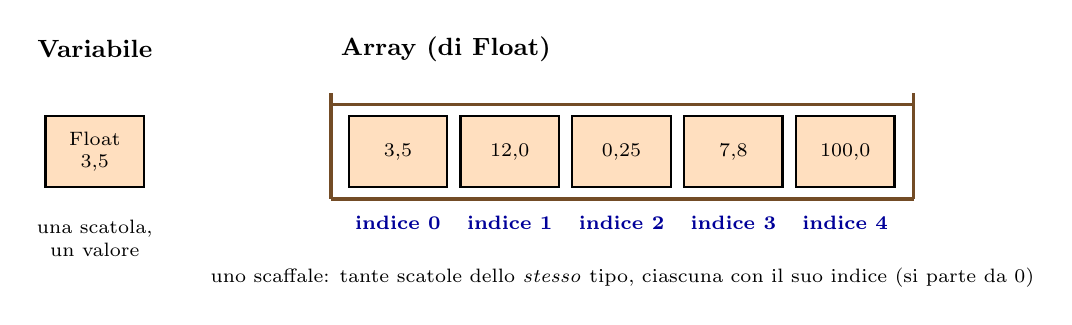
\begin{tikzpicture}[font=\footnotesize,
  ue7box/.style={draw, thick, fill=orange!25, minimum width=1.25cm, minimum height=0.9cm,
                 align=center, font=\scriptsize},
  ue7shelf/.style={draw, very thick, brown!60!black}]
  % variabile singola
  \node[font=\small\bfseries] at (0,2.3) {Variabile};
  \node[ue7box] (v) at (0,1.0) {Float\\3,5};
  \node[font=\scriptsize, align=center] at (0,-0.1) {una scatola,\\un valore};
  % array
  \begin{scope}[xshift=3.0cm]
    \node[font=\small\bfseries, anchor=west] at (0,2.3) {Array (di Float)};
    \draw[ue7shelf] (0,0.4) -- (7.4,0.4);
    \draw[ue7shelf] (0,1.6) -- (7.4,1.6);
    \draw[ue7shelf] (0,0.4) -- (0,1.75);
    \draw[ue7shelf] (7.4,0.4) -- (7.4,1.75);
    \node[ue7box] at (0.85,1.0) {3,5};
    \node[ue7box] at (2.27,1.0) {12,0};
    \node[ue7box] at (3.69,1.0) {0,25};
    \node[ue7box] at (5.11,1.0) {7,8};
    \node[ue7box] at (6.53,1.0) {100,0};
    \foreach \x/\i in {0.85/0, 2.27/1, 3.69/2, 5.11/3, 6.53/4} {
      \node[font=\scriptsize\bfseries, text=blue!60!black] at (\x,0.1) {indice \i};
    }
    \node[font=\scriptsize, align=center] at (3.7,-0.6) {uno scaffale: tante scatole
      dello \emph{stesso} tipo, ciascuna con il suo indice (si parte da 0)};
  \end{scope}
\end{tikzpicture}
\caption{La metafora del docente. Una variabile è una scatola che contiene un valore; un
array è uno scaffale che contiene tante scatole dello stesso tipo. Ogni posto dello
scaffale ha un indice, e il primo indice è 0. Schema ricostruito.}
\label{ue7:fig:scaffale}
\end{figure}

\paragraph{Approfondimento: array, set e map.} Romero e Sewell (capitolo 13, ``Data
Structures and Flow Control'') chiamano \textbf{contenitori} (\emph{containers}) le
strutture che raccolgono più valori dello stesso tipo, e nei Blueprint ce ne sono tre.
L'\textbf{array} è una lista ordinata con accesso per \textbf{indice}, ``e gli array
partono sempre dall'indice 0'': con quattro elementi, il primo ha indice 0 e l'ultimo
indice 3, cioè \emph{Length}~$-$~1. Il \textbf{set} è un insieme senza ordine e senza
doppioni, in cui si cerca per valore; la \textbf{map} associa a ogni \emph{chiave} un
\emph{valore} (per esempio il nome di un'arma e le sue munizioni). Sugli array si lavora
con una manciata di nodi: \textbf{Get (a copy)} legge l'elemento a un indice,
\textbf{Set Array Elem} lo modifica, \textbf{Add} aggiunge in fondo, \textbf{Insert}
inserisce a un indice spostando gli altri, \textbf{Length} e \textbf{Last Index} dicono
quanto è lungo, \textbf{Random Array Item} pesca un elemento a caso. Gli autori
avvertono: mai leggere un indice oltre l'ultimo, perché i risultati sono imprevedibili.
La tabella~\ref{ue7:tab:contenitori} riassume i quattro modi in cui una variabile può
essere costituita.

% ---------------------------------------------------------------------
\section{L'ereditarietà: parent e child}
\label{ue7:sec:ereditarieta}

La slide successiva riprende rapidamente le collisioni (``ripasseremo anche un po' le
collisioni'') e introduce il secondo concetto della giornata. ``Qualcuno di voi ha mai
sentito parlare dei concetti di \textbf{parent} e \textbf{child} in programmazione?''

\paragraph{Padre e figlio.} ``Mettiamo un esempio che possiamo vedere nella vita di tutti
i giorni'': il rapporto fra genitori e figli. ``Io, come figlio di mio padre, ho preso
una parte dei geni di mio padre'' (e di mia madre), ``e però, come essere unico, posso
variare nelle mie particolarità: non sono uguale, ma condivido comunque delle cose''.
Lo stesso succede con gli oggetti: ``ci sono degli oggetti che possono essere figli di
altri oggetti''. Esempio: un cubo \emph{parent} che nel Begin Play stampa un valore, e
fa solo quello. ``Il child mi stamperà sempre quel valore, ma magari stampa anche un
altro valore'': ``prende la caratteristica del papà, ma volendo può aggiungere, o
addirittura \textbf{sovrascrivere}, alcune azioni''.

\paragraph{Il cubo che diventa cilindro.} In Unreal i child si creano direttamente
dall'engine. In slide c'è il BP\_Cube delle lezioni precedenti: ``vogliamo farlo
diventare un cilindro? Creiamo un child e cambiamo semplicemente la Static Mesh''. ``Il
parent rimarrà un cubo, invece il figlio ha voluto cambiare forma'': per le
caratteristiche di Blueprint avranno lo stesso comportamento, ``oppure, volendo, lo
possiamo anche cambiare''. La figura~\ref{ue7:fig:gerarchia} mostra la gerarchia che si
costruirà oggi.

\begin{figure}[htbp]
\centering
\begin{tikzpicture}[font=\footnotesize,
  ue7cls/.style={draw, thick, rounded corners=4pt, align=center, fill=gray!8,
                 text width=3.3cm, minimum height=1.0cm, inner sep=4pt},
  ue7inh/.style={-{Triangle[open, length=3mm, width=3mm]}, thick}]
  \node[ue7cls, fill=gray!20] (actor) at (0,3.0) {\textbf{Actor}\\(classe di Unreal)};
  \node[ue7cls, fill=blue!10] (act) at (0,1.0) {\textbf{BP\_Activable}\\eventi
    Activation e Deactivation (Print String)};
  \node[ue7cls, fill=yellow!25] (light) at (-4.4,-1.4) {\textbf{BP\_ActivableLight}\\Point
    Light; override: accende e spegne};
  \node[ue7cls, fill=green!12] (ball) at (0,-1.4) {\textbf{BP\_BallMoving}\\(esercizio)
    override: Play e Reverse};
  \node[ue7cls, fill=orange!15] (plat) at (4.4,-1.4) {\textbf{piattaforma
    attivabile}\\(esercizio e compito)};
  \node[ue7cls, fill=gray!8] (btn) at (5.2,3.0) {\textbf{BP\_Button}\\array
    ActivableItems di tipo BP\_Activable};
  \draw[ue7inh] (act) -- (actor);
  \draw[ue7inh] (light.north) -- ++(0,0.6) -| (act.south);
  \draw[ue7inh] (ball) -- (act);
  \draw[ue7inh] (plat.north) -- ++(0,0.6) -| (act.south);
  \draw[ue7inh] (btn) -- (actor);
  \draw[-{Stealth[length=2.2mm]}, thick, dashed, violet!60!black] (btn.south) to[bend
    left=10] node[pos=0.45, right, font=\scriptsize, align=left]{contiene referenze\\a
    qualunque child} (act.east);
\end{tikzpicture}
\caption{La gerarchia di classi costruita nella lezione. Le frecce con la punta vuota
vanno dal child al parent (``eredita da''). BP\_Activable definisce i due eventi comuni;
ogni child li ridefinisce a modo suo. BP\_Button tiene un array di referenze di tipo
BP\_Activable, e quindi può contenere qualunque child. I nomi dei Blueprint
dell'esercizio sono quelli suggeriti dal docente; schema ricostruito.}
\label{ue7:fig:gerarchia}
\end{figure}

\paragraph{Approfondimento: superclasse, sottoclasse e tipo.} Romero e Sewell (capitolo
3, ``Object-Oriented Programming and the Gameplay Framework'') danno la versione
tecnica. Quando si crea un Blueprint, la prima cosa che si sceglie è la sua
\textbf{classe parent} (la \emph{superclasse}); un Blueprint ha \emph{un solo} parent,
ma può avere molti child (\emph{sottoclassi}). Il loro esempio sono le armi: una classe
base \emph{Weapon} con tutto ciò che è comune, e le armi concrete come figlie. Il
vantaggio è doppio. Da un lato, una funzione definita nel parent (\emph{Fire}) può
essere \textbf{ridefinita} (\emph{override}) in ogni child (il fucile a energia spara un
raggio, il lanciarazzi un razzo), e a runtime viene eseguita la versione della classe
effettiva dell'oggetto. Dall'altro, un child \textbf{è anche} del tipo del parent:
un'istanza del lanciarazzi è un \emph{Weapon}, e una variabile o un parametro di tipo
Weapon può contenerla. È esattamente il trucco su cui si regge il pulsante di oggi: una
variabile di tipo \emph{BP\_Activable} potrà contenere una luce, una piattaforma, una
palla, qualunque child degli attivabili. Del resto, ogni Blueprint della lezione è già un
child: BP\_Button ha come parent la classe \emph{Actor}.

% ---------------------------------------------------------------------
\section{La dimostrazione: il pulsante finito}
\label{ue7:sec:demo}

``Andremo a creare un bellissimo pulsantone. Eccolo qua.'' Nella scena del docente c'è
il risultato finale. Il giocatore sale sulla pedana, la pedana si abbassa e
\textbf{accende una luce} (``vedremo anche un pochino di \emph{lighting}''); se scende,
la luce si spegne. Nella stessa scena c'è una piattaforma che reagisce allo stesso
pulsante: ``ho creato una piattaforma di tipologia \textbf{attivabile}'', e luce e
piattaforma ``condividono'' qualcosa, ``sono della stessa classe, ma comportamenti
diversi''. Collegata la piattaforma al pulsante, la pressione accende la luce
\emph{e} manda giù la piattaforma; ``in questo caso ho fatto sì che andasse solo giù'':
quando la piattaforma è in basso ci si sale sopra, e lei torna su; si torna sul
pulsante, e di nuovo giù.

\paragraph{La domanda sull'interazione.} ``Faremo anche le interazioni, tipo premi E per
interagire?'' Sì: la prossima lezione sarà sulle \textbf{animazioni}, con un personaggio
animato, e l'interazione si farà con il \textbf{trace}, ``infatti il trace è collegato
al fatto dell'interazione'': ha interagito o non ha interagito.

\paragraph{Approfondimento: overlap o tasto?} I due modi di attivare qualcosa hanno usi
diversi. L'\emph{overlap} di un volume, quello di oggi, è passivo: scatta perché il
giocatore \emph{è} in un posto (pedane a pressione, trappole, cutscene). L'interazione
con un tasto è attiva: il giocatore guarda un oggetto e preme. Lo schema tipico, che la
lezione annuncia, è un \emph{line trace} dalla telecamera in avanti, eseguito alla
pressione del tasto; se colpisce un actor che ``sa'' interagire, gli si chiama un evento.
Per chiamarlo senza sapere in anticipo che classe abbia l'oggetto colpito si usa di
solito una \textbf{Blueprint Interface} (Romero e Sewell, capitolo 16): una lista di
funzioni senza corpo, che ogni classe interessata implementa a modo suo. È una cugina
dell'ereditarietà vista oggi, utile quando le classi da accomunare non hanno un parent
comune.

% ---------------------------------------------------------------------
\section{Il pulsante: due mesh e una box}
\label{ue7:sec:bottone}

``Allora, ragazzi, vi chiedo se siete pronti con il vostro progettino.'' Prima di
cominciare, la raccomandazione di sempre: tenere il progetto ordinato in
\textbf{cartelle}, ``perché se no un giorno succederà che non ritroverete'' le cose,
``come perdere qualcuno in un centro commerciale il sabato''. Nella cartella
\emph{Blueprint}, ``siamo al solito'': Blueprint Class, Actor. Il docente lo chiama
\textbf{BP\_Button1} (``io farò sempre il mio bellissimo BP\_Button1''); nel capitolo è
BP\_Button.

\paragraph{Due Static Mesh, non una.} ``Il bottone, per come sono fatte le mesh, sono due
Static Mesh'': una è il \textbf{frame}, la cornice, e l'altra la \textbf{piastra} che si
abbassa. Il docente le crea con Ctrl+C e Ctrl+V da un componente Static Mesh, e le
rinomina \textbf{Frame} e \textbf{Platform}; nel campo \emph{Static Mesh} assegna alla
prima la mesh della cornice della pedana a pressione (``se non sbaglio \emph{pressure
plate frame}'') e alla seconda quella della piastra (``\emph{pressure plate}\ldots{}
platform''); i nomi esatti degli asset nel progetto del corso non sono sicuri dalla
trascrizione. ``Essendo che sono fatti all'unisono'', i due pezzi sono già allineati.

\paragraph{Un consiglio per i 3D artist.} Il motivo della divisione vale per chiunque
modelli, o faccia modellare, oggetti interattivi. ``Se dovete fare un pulsante, non fate
fare un pulsante unico: fate fare un pulsante che è diviso'' fra la cornice (``quello che
sta attorno'') e la \emph{pressure plate}. ``Perché se adesso andiamo ad abbassare, ed è
un unico asset, tutto il bottone va giù, anche il frame, quindi si va a compenetrare col
pavimento.'' La regola: ``se ci sono delle cose interagibili a livello di movimentazione,
sappiate che è meglio sempre \textbf{splittarle}''. Poi, certo, ``dipende dalla
creatività'' e dal designer.

\paragraph{La box.} Terzo componente, ``la mitica'' \textbf{Box Collision}, scalata
perché sia ``leggermente unanime'' con il bottone, cioè della sua stessa impronta, e
alzata sull'asse Z: ``ricordatevi, attenzione a sotto''. E soprattutto, come per la
piattaforma della volta scorsa, \textbf{figlia della Platform}: ``la box deve seguire la
platform. Importante, in modo tale che se io sposto, si sposta con essa''
(figura~\ref{ue7:fig:bottone}).

\paragraph{È la box a comandare.} Una studentessa chiede conferma: ``bisogna fare la box
sopra perché è la box che interagisce, giusto?'' Sì: il player entra con i piedi nella
box, la box interagisce, la timeline parte e il pulsante va giù. ``Non è tanto la
piattaforma o il pulsante a triggerare l'evento, ma la box sopra.'' E perché non usare
l'overlap della mesh stessa? ``Perché le collisioni sono \textbf{troppo precise}'': sono
``a contatto con una superficie'', ``un controllo sempre più micro'', ``forse sì, forse
no'', e ``la possibilità di errore è molto più ampia''. Un volume, invece, dà una
risposta macro: ``sì, no''.

\begin{figure}[htbp]
\centering
\begin{tikzpicture}[font=\footnotesize,
  ue7comp/.style={draw, thick, rounded corners=3pt, align=left, fill=gray!8,
                  minimum height=0.6cm, text width=3.4cm, inner sep=4pt},
  ue7tree/.style={thick, gray!70!black}]
  \node[font=\small\bfseries, anchor=west] at (-0.2,1.0) {Components di BP\_Button};
  \node[ue7comp, anchor=west] (root) at (0,0.2) {DefaultSceneRoot};
  \node[ue7comp, anchor=west, fill=gray!20] (fr) at (0.6,-0.6) {\textbf{Frame}
    (Static Mesh)};
  \node[ue7comp, anchor=west, fill=blue!10] (pl) at (0.6,-1.4) {\textbf{Platform}
    (Static Mesh)};
  \node[ue7comp, anchor=west, fill=green!12] (bx) at (1.2,-2.2) {\textbf{Box} (Box
    Collision)};
  \node[ue7comp, anchor=west, fill=red!10] (tl) at (0,-3.0) {\textbf{PushButton}
    (Timeline)};
  \draw[ue7tree] (0.2,-0.1) |- (fr.west);
  \draw[ue7tree] (0.2,-0.1) |- (pl.west);
  \draw[ue7tree] (0.8,-1.7) |- (bx.west);
  % vista laterale
  \begin{scope}[xshift=7.4cm, yshift=-1.3cm]
    \draw[thick, gray] (-1.2,-1.0) -- (4.4,-1.0);
    \node[font=\scriptsize, gray] at (3.9,-1.25) {pavimento};
    \fill[gray!45, draw=black, thick] (-0.1,-1.0) rectangle (3.1,-0.75);
    \node[font=\scriptsize] at (1.5,-1.25) {Frame};
    \fill[blue!25, draw=blue!50!black, thick] (0.2,-0.75) rectangle (2.8,-0.5);
    \draw[thick, dashed, blue!50!black] (0.2,-0.85) rectangle (2.8,-0.6);
    \node[font=\scriptsize, anchor=west] at (3.2,-0.55) {Platform};
    \draw[-{Stealth[length=1.6mm]}, thick, red!60!black] (1.5,-0.45) -- (1.5,-0.72);
    \node[font=\scriptsize, red!60!black, anchor=west] at (1.6,-0.25) {$-10$ su Z};
    \draw[thick, dashed, green!50!black, fill=green!8, fill opacity=0.6]
      (0.3,-0.5) rectangle (2.7,0.15);
    \node[font=\scriptsize, green!40!black] at (1.0,-0.17) {Box};
    % omino
    \draw[thick] (-0.7,0.35) circle (0.13);
    \draw[thick] (-0.7,0.22) -- (-0.7,-0.35);
    \draw[thick] (-0.7,-0.35) -- (-0.85,-1.0);
    \draw[thick] (-0.7,-0.35) -- (-0.55,-1.0);
    \node[font=\scriptsize] at (-0.7,0.7) {player};
  \end{scope}
\end{tikzpicture}
\caption{I componenti del pulsante. A sinistra la gerarchia: Frame e Platform sono due
Static Mesh separate; la Box Collision è figlia della Platform, così la segue; la
timeline PushButton compare tra i componenti. A destra la vista laterale: la piastra
scende di 10 unità dentro la cornice (tratteggio), mentre la cornice resta ferma.
Schema ricostruito; le proporzioni non sono quelle dell'asset.}
\label{ue7:fig:bottone}
\end{figure}

% ---------------------------------------------------------------------
\section{Le collisioni della Static Mesh: simple e complex}
\label{ue7:sec:collisioni}

``Poi, se non sbaglio, su questo asset c'è un problema.'' È quello sollevato a inizio
lezione: il pulsante, come la piattaforma, potrebbe avere ``una collisione un po' tanto
alta'' per il personaggio.

\paragraph{Il Max Step Height.} Nel personaggio del giocatore c'è una variabile,
\textbf{Max Step Height}, ``che non ci permette di andare sopra queste tipologie di
asset'' se sono più alte di un certo valore. Il docente prova sulla sua scena: a lui va
``benissimo'', ``perché guardate cosa ho fatto io per ovviare a questo problema''. A
qualcuno degli studenti il personaggio si blocca con i piedi? Pare di no, ``bene''; ma
``per accortezza'', visto che al docente è capitato, si sistema la collisione della mesh.

\paragraph{Approfondimento: Max Step Height e Walkable Floor.} I due parametri stanno nel
\emph{Character Movement Component} del personaggio. Il \textbf{Max Step Height}
(predefinito 45 unità, cioè 45 centimetri) è l'altezza massima di uno ``scalino'' che il
personaggio può salire camminando, senza saltare; il \textbf{Walkable Floor Angle}
(predefinito 44,765 gradi) è la pendenza massima su cui può camminare. Se il bordo della
collisione di un oggetto supera lo scalino, la capsula del personaggio ci sbatte contro
come contro un muro. Si può alzare lo scalino del personaggio, ma cambia il modo in cui
si muove ovunque; di solito conviene sistemare la collisione dell'oggetto, come fa la
lezione.

\paragraph{L'editor della Static Mesh.} Si seleziona la mesh della piastra e si clicca
sulla ``finestrella blu'', l'icona dell'asset nel campo Static Mesh, per aprire
l'\textbf{editor della Static Mesh}: ``la schermata in cui Unreal fa vedere tutte le
particolarità delle collisioni dell'asset stesso'', ``dati molto più \emph{insight} del
modello''.

\paragraph{Una parentesi sui LOD.} Fra i dati ci sono i \textbf{LOD}, i \emph{level of
detail}: ``quella pratica di abbassare la risoluzione degli asset quando sono distanti,
in modo tale da avere ottimizzazione''. ``Sono tipo a 200 metri da me? Abbassa la
qualità, perché pesa.'' Il corso non li userà, ma è bene sapere che esistono.

\paragraph{Simple e complex.} Dal menù \textbf{Show} in alto si visualizzano le
collisioni dell'asset, e ``ci sono due tipologie di collisioni''.
\begin{itemize}
  \item Le \textbf{simple}, in \textbf{verde}: forme semplici, ``usate per avere
        interazioni di base''. Sono quelle che Unreal usa normalmente quando si mette un
        asset nella viewport, ``per tempi e cose di ottimizzazione''.
  \item Le \textbf{complex}, ``questi lineamenti blu'' (azzurri): la forma esatta del
        modello, triangolo per triangolo. Servono quando ``ci serve l'esatto punto''
        in cui si tocca l'oggetto. Esempio: un \textbf{sistema di scalata}, in cui
        ``devo andare a vedere il punto esatto in cui ho messo la mano'' per tirare su il
        personaggio (``poi ci sono anche alternative'').
\end{itemize}
Le due collisioni si preparano ``durante la modellazione'', e chi segue il corso di 3D
art le vedrà. Ma attenzione: ``se mettete le complex collision su tutti gli asset,
probabilmente potete dire ciao al vostro bellissimo PC'', a meno di ottimizzazioni
parallele. Qui servono le simple.

\paragraph{Modificare la collisione.} La cosa bella è che le collisioni simple si
possono modificare a mano. Cliccando sul ``reticoletto verde'' si possono muovere,
ruotare e scalare come un oggetto qualsiasi. Gli studenti dovrebbero avere una
collisione ``un po' più arzigogolata'', ``con tutti i reticolini''; il docente ha già
modificato la sua. La procedura:
\begin{enumerate}
  \item \textbf{cancellare} la collisione simple esistente, ``quella verde, non quella
        azzurra'';
  \item dal menù \textbf{Collision} aggiungerne una nuova, scegliendo fra
        \textbf{Sphere}, \textbf{Capsule}, \textbf{Box} e le varie \textbf{k-DOP} (10DOP-X,
        Y, Z, 18DOP, 26DOP; nella trascrizione ``10 di OP meno X'');
  \item per il pulsante, \textbf{Box} (``Box Simplified Collision''): ``a noi ci serve
        una scatoletta, è un quadrato alla fine'';
  \item selezionare la box e \textbf{stringerla} ``proprio un'anticchia'', abbassandola,
        dopo aver tolto lo \emph{snap}, ``quasi come se fosse una collisione già
        abbassata''.
\end{enumerate}
Ora il pulsante ``ha una collisione un po' più affondabile''.

\paragraph{Le forme a confronto.} Il docente prova le alternative una per una. La
\textbf{sfera} su una piastra quadrata ``non ci serve assolutamente, perché non è
coerente alla sua forma''. Le \textbf{k-DOP} invece seguono il modello con un numero
crescente di piani: ``sono il livello di dettaglio che la collisione avrà, il livello di
vertici''; ``più vertici ci sono, più le collisioni sono precise, meno spigolose''. Sul
cubetto la 10DOP sulla X, sulla Y e sulla Z danno risultati quasi uguali, con ``piccole
differenze'' di taglio; la 18DOP ``ha fatto gli angoli più precisi''; la 26DOP, ``il
massimo'', taglia anche gli spigoli (figura~\ref{ue7:fig:kdop}).

\paragraph{Un'esperienza di lavoro.} ``A me è capitato con un lavoro che ho fatto.'' Nel
livello c'era una piccola pista, e alcuni asset avevano collisioni ``estremamente
complesse'': il docente e il gruppo di designer hanno dovuto \textbf{cancellare tutte le
collisioni e rifarle} a mano, ``con i cubettini'', per semplificare il lavoro
dell'engine. La morale: le collisioni sono parte del lavoro del level designer, non solo
del modellatore.

\begin{figure}[htbp]
\centering
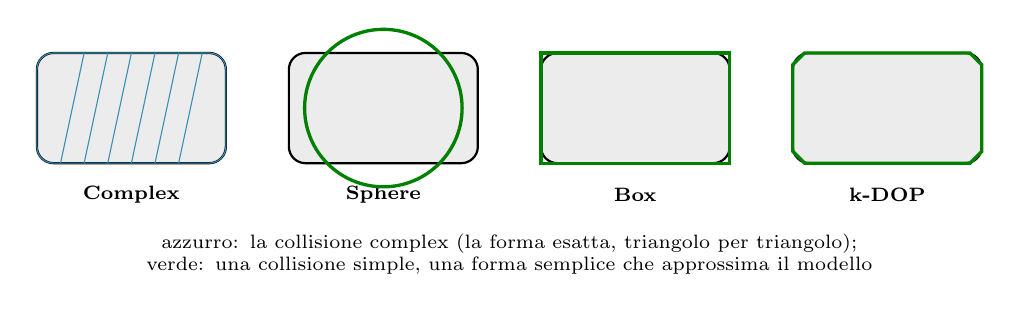
\begin{tikzpicture}[font=\footnotesize,
  ue7mesh/.style={draw=black, thick, fill=gray!15},
  ue7coll/.style={draw=green!50!black, very thick},
  ue7cplx/.style={draw=cyan!70!black, thin}]
  % modello: piastra con bordi smussati (vista dall'alto, stilizzata)
  \foreach \x/\nome in {0/Complex, 3.2/Sphere, 6.4/Box, 9.6/k-DOP} {
    \begin{scope}[xshift=\x cm]
      \draw[ue7mesh, rounded corners=6pt] (0,0) rectangle (2.4,1.4);
      \node[font=\scriptsize\bfseries] at (1.2,-0.4) {\nome};
    \end{scope}
  }
  % complex: segue tutto
  \draw[ue7cplx, rounded corners=6pt] (0,0) rectangle (2.4,1.4);
  \foreach \i in {0.3,0.6,...,2.1} {\draw[ue7cplx] (\i,0) -- (\i+0.3,1.4);}
  % sphere
  \draw[ue7coll] (4.4,0.7) circle (1.0);
  % box
  \draw[ue7coll] (6.4,0) rectangle (8.8,1.4);
  % kdop: ottagono
  \draw[ue7coll] (9.75,0) -- (11.85,0) -- (12.0,0.15) -- (12.0,1.25) -- (11.85,1.4)
    -- (9.75,1.4) -- (9.6,1.25) -- (9.6,0.15) -- cycle;
  \node[font=\scriptsize, align=center, text width=12cm] at (6.0,-1.15) {azzurro: la
    collisione complex (la forma esatta, triangolo per triangolo); verde: una collisione
    simple, una forma semplice che approssima il modello};
\end{tikzpicture}
\caption{Collisioni della piastra viste dall'alto, in forma stilizzata. La complex
segue ogni triangolo del modello; la Sphere non è coerente con la forma; la Box è la
scelta della lezione; le k-DOP aggiungono piani e smussano gli spigoli. Schema
ricostruito, non una schermata dell'editor.}
\label{ue7:fig:kdop}
\end{figure}

\paragraph{Approfondimento: Collision Complexity.} Nell'editor della Static Mesh, fra
i dettagli dell'asset, c'è l'impostazione \textbf{Collision Complexity}. Con il
valore predefinito (\emph{Project Default}, in pratica ``simple e complex separate'') le
query fisiche e il movimento dei personaggi usano la collisione simple, mentre i trace
che lo chiedono esplicitamente (il flag \emph{Trace Complex}) usano quella complex. Con
\emph{Use Complex Collision As Simple} la forma esatta viene usata per tutto: comodo per
un pavimento irregolare statico, ma costoso, e incompatibile con la simulazione fisica
dell'oggetto. Le k-DOP (\emph{discrete oriented polytope}) sono poliedri convessi che
racchiudono la mesh con 10, 18 o 26 piani a orientamento fisso; il menù
\emph{Collision} offre anche \emph{Auto Convex Collision}, che scompone la mesh in più
pezzi convessi, una via di mezzo fra la precisione della complex e il costo della
simple.

% ---------------------------------------------------------------------
\section{La timeline del pulsante}
\label{ue7:sec:timeline}

``Fatto questo, ritorniamo sul nostro bellissimo button e andiamo effettivamente a creare
quello che sarà il funzionamento di base'': il tasto si deve abbassare sulla Z.

\paragraph{Gli eventi e il controllo sul player.} ``Quello che abbiamo visto l'altra
volta'': con la Box selezionata, nella sezione degli eventi in fondo ai dettagli, si
creano \textbf{On Component Begin Overlap} e \textbf{On Component End Overlap}, ``tutti e
due''. Poi ``la solita cosa'': si verifica che sia il player, ``con Is Valid o con il
tag, ma noi facciamo più semplice''. Dall'\textbf{Other Actor} si tira fuori un
\textbf{==} (``uguale uguale'') con \textbf{Get Player Pawn}, e il risultato va in un
\textbf{Branch}.

\paragraph{La timeline.} Dal ramo True, ``abbiamo già detto che è una timeline quella
che useremo'': una nuova timeline, rinominata \textbf{PushButton}, avviata con
\textbf{Play from Start} (la differenza con Play si chiarirà nella
sezione~\ref{ue7:sec:play}). Quanto deve scendere il pulsante? Il docente lo misura
nella viewport: seleziona la piastra, attiva lo \emph{snap} (``molto meglio''), con passo
10, e la abbassa finché è ``totalmente abbassata''. Bastano \textbf{10 unità}: ``quindi
abbiamo capito che dovremmo abbassarla di 10''.

\paragraph{La curva.} Doppio clic sulla timeline. ``Il valore da mettere per la
lunghezza della timeline è \textbf{0,25 secondi}. È molto corto.'' Poi:
\begin{enumerate}
  \item una \textbf{float track};
  \item un punto (Shift e clic) a \textbf{tempo 0, valore 0};
  \item un secondo punto a \textbf{tempo 0,25} (``il massimo della nostra timeline'') e
        \textbf{valore $-$10}: ``farà un passaggio in 0,25 secondi da 0 a $-$10'';
  \item i due pulsantini \textbf{Zoom to Fit Horizontal} e \textbf{Zoom to Fit
        Vertical} (``le due freccine''), che adattano il grafico alla lunghezza e
        all'altezza della curva.
\end{enumerate}
Una domanda dalla chat (``come si chiama il pallino sulla timeline?'') riceve la risposta
già nota: Shift e clic. Rispetto alla piattaforma della volta scorsa c'è una differenza
importante: allora la traccia andava da 0 a 1 ed era un \emph{alfa} da dare a un Lerp;
oggi la traccia contiene \emph{direttamente} lo spostamento, in unità del mondo.

\paragraph{Il nome della traccia.} ``Abbiamo la New Track 0'': la si rinomina cliccandoci
sopra con \textbf{F2}, \textbf{PushButtonZ} (``facciamo una Z maiuscola''). Il pin sul
nodo prende lo stesso nome; a una studentessa resta scritto \emph{New Track 0} anche
dopo la rinomina, e il docente la rassicura: ``è solo il nome che gli abbiamo dato'', il
funzionamento non cambia.

\paragraph{Il movimento.} Nell'Event Graph:
\begin{itemize}
  \item dal pin \textbf{PushButtonZ} si crea un \textbf{Make Vector}, collegando il
        valore alla \textbf{Z} (``l'asse che ci interessa''); X e Y restano a 0, ``tanto
        la X è zero e rimane zero'';
  \item si trascina la Platform nel grafo e se ne tira fuori \textbf{Set Relative
        Location}, con il vettore in \emph{New Location}. ``È relative perché è
        relativa alla sua transform'': lo zero è quello della piastra dentro il
        Blueprint, non lo zero del mondo;
  \item il nodo va collegato all'\textbf{Update} della timeline.
\end{itemize}
In Play, sulla pedana, ``non esplode, vedete che si abbassa''. Ma non si rialza più:
``è normale''. Manca il ritorno: dall'\textbf{End Overlap}, con lo stesso controllo sul
player, si collega l'ingresso \textbf{Reverse} della timeline. ``Premuto, torna su;
premuto, torna su.'' ``Eccolo che abbiamo creato il nostro movimento del pulsante, non
ancora la sua funzionalità'' (figura~\ref{ue7:fig:grafobottone}).

\begin{figure}[htbp]
\centering
\begin{tikzpicture}[font=\footnotesize,
  ue7node/.style={draw, thick, rounded corners=4pt, align=center, fill=gray!8,
                  minimum height=0.8cm, text width=2.0cm},
  ue7ev/.style={ue7node, fill=red!12},
  ue7exec/.style={-{Stealth[length=2.5mm]}, very thick, black!80},
  ue7data/.style={-{Stealth[length=2mm]}, thick, violet!60!black}]
  \node[ue7ev, text width=2.6cm] (bo) at (0,1.2) {\textbf{On Component Begin
    Overlap} (Box)};
  \node[ue7ev, text width=2.6cm] (eo) at (0,-1.2) {\textbf{On Component End
    Overlap} (Box)};
  \node[ue7node, text width=1.9cm] (eq1) at (3.3,2.6) {Other Actor \textbf{==} Get
    Player Pawn};
  \node[ue7node, text width=1.3cm] (br1) at (3.3,1.2) {\textbf{Branch}};
  \node[ue7node, text width=1.3cm] (br2) at (3.3,-1.2) {\textbf{Branch}};
  \node[ue7node, text width=1.9cm] (eq2) at (3.3,-2.6) {Other Actor \textbf{==} Get
    Player Pawn};
  \node[ue7node, fill=red!8, text width=2.4cm, minimum height=2.6cm] (tl) at (7.3,0)
    {\textbf{Timeline}\\PushButton\\[2pt]\scriptsize 0,25 s\\da 0 a $-$10};
  \node[ue7node, text width=1.6cm] (mv) at (10.6,-1.4) {\textbf{Make Vector}\\X 0, Y 0};
  \node[ue7node, text width=2.3cm] (set) at (13.1,0.8) {Platform $\rightarrow$
    \textbf{Set Relative Location}};
  \draw[ue7exec] (bo) -- (br1);
  \draw[ue7exec] (eo) -- (br2);
  \draw[ue7data] (eq1) -- (br1);
  \draw[ue7data] (eq2) -- (br2);
  \draw[ue7exec] (br1.east) -- node[above, font=\scriptsize]{True} ++(0.7,0) |-
    node[pos=0.78, above, font=\scriptsize]{Play from Start} ([yshift=0.8cm]tl.west);
  \draw[ue7exec] (br2.east) -- node[below, font=\scriptsize]{True} ++(0.7,0) |-
    node[pos=0.78, below, font=\scriptsize]{Reverse} ([yshift=-0.8cm]tl.west);
  \draw[ue7exec] ([yshift=0.8cm]tl.east) -- node[above, font=\scriptsize]{Update}
    (set.west);
  \draw[ue7data] ([yshift=-0.6cm]tl.east) -- node[above, font=\scriptsize, pos=0.5]{PushButtonZ}
    ++(0.6,0) |- (mv.west);
  \draw[ue7data] (mv.east) -| node[pos=0.3, below, font=\scriptsize]{Z $\rightarrow$
    New Location} (set.south);
\end{tikzpicture}
\caption{Il movimento del pulsante. Il Begin Overlap della Box, se l'actor è il player,
fa partire la timeline PushButton da capo; l'End Overlap la manda in Reverse. A ogni
Update il valore della traccia (da 0 a $-$10 in 0,25 secondi) diventa la Z di un
vettore, e la piastra si sposta con Set Relative Location. Schema ricostruito.}
\label{ue7:fig:grafobottone}
\end{figure}

\paragraph{Approfondimento: perché qui niente Lerp.} La sesta lezione aveva mostrato il
metodo ``giusto'' per la piattaforma: una traccia da 0 a 1 usata come alfa di un Lerp
fra due posizioni salvate. Qui il docente sceglie la strada diretta, e funziona per due
ragioni. La prima: il valore della traccia è \emph{assoluto}, non si somma alla posizione
corrente, quindi non si accumula (era il difetto del primo metodo della volta scorsa).
La seconda: la piastra è figlia di una radice ferma, e la sua posizione relativa di
partenza è (0, 0, 0), quindi ``$-$10 rispetto alla radice'' vuol dire esattamente ``10
più in basso di dove sta''. Se la piastra fosse stata spostata nel Blueprint, per
esempio a Z 5, il primo Update la teletrasporterebbe a Z 0: in quel caso serve sommare
lo spostamento alla posizione iniziale salvata, o tornare al Lerp. Per oggetti che si
spostano di poco, una traccia in unità del mondo è la soluzione più leggibile.

% ---------------------------------------------------------------------
\section{Le curve: linear e auto}
\label{ue7:sec:curve}

``Adesso vi faccio vedere anche una particolarità, che potremmo usare anche per la
piattaforma'': si può \textbf{modificare la tipologia dei punti}.

\paragraph{Lineari.} I punti creati finora sono \textbf{lineari}: ``formano una linea'',
e l'aumento o la diminuzione del valore ``è sempre costante'' nel tempo: in ogni
frazione di secondo il valore cambia sempre della stessa quantità, ``tra un punto e
l'altro''.

\paragraph{Curve.} ``Se invece vogliamo una curva un po' più \emph{smooth}'', si fa tasto
destro su un punto: compare la serie di \textbf{Key Interpolation}, ``cioè ti dice: quale
tipo di punto vuoi che sia?''. Il docente sceglie \textbf{Auto}, e la linea diventa una
curva; lo stesso sull'altro punto. Ora, con i ``piccoli braccetti'' (le tangenti) di
ciascun punto, si può modellare ``come nel tempo questa linea va da punto A a punto B''
(figura~\ref{ue7:fig:curve}, tabella~\ref{ue7:tab:interp}).

\paragraph{A che cosa serve.} Una studentessa chiede che cosa cambi in pratica. Il
docente prova: allunga la timeline a 1 secondo e piega la curva in modo che superi il
valore finale e poi ci ritorni. Il risultato, con un'escursione di appena 10 unità, sono
``micro movimenti'': il pulsante ``fa boom e ritorna su'', ``su e giù e si abbassa''.
``Cambiare la forma della curva ci permette di creare dei piccoli intervalli di vario
tipo'': il movimento rallenta, accelera, rimbalza. Su un pulsante si vede poco (``è molto
piccolo come spazio''); ``magari in pausa'' il docente propone di mostrarlo con ``una
piccola sferetta che fa su e giù''. Poi rimette la curva com'era.

\begin{figure}[htbp]
\centering
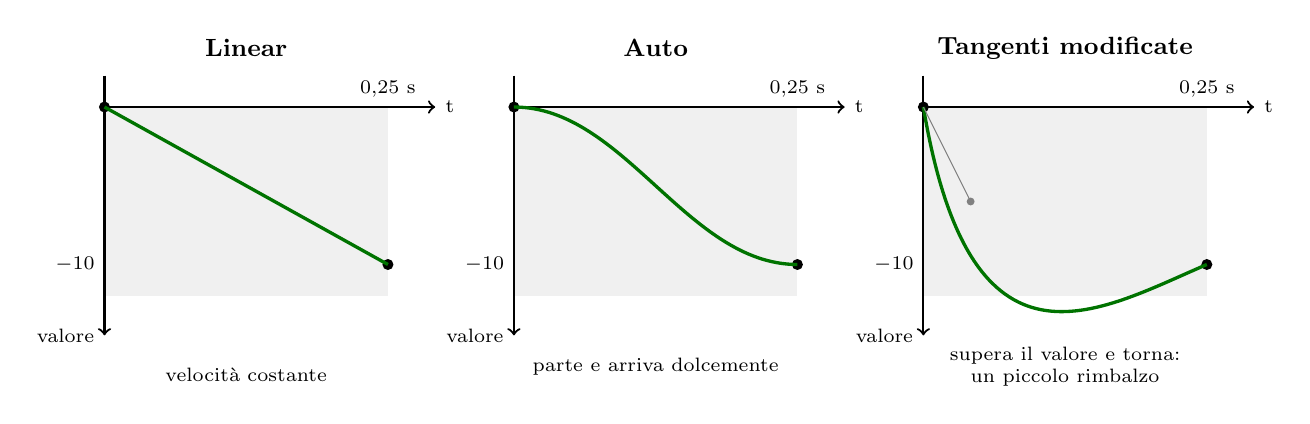
\begin{tikzpicture}[font=\footnotesize]
  \foreach \x/\titolo in {0/Linear, 5.2/Auto, 10.4/Tangenti modificate} {
    \begin{scope}[xshift=\x cm]
      \fill[gray!12] (0,-2.4) rectangle (3.6,0);
      \draw[->, thick] (0,0) -- (4.2,0) node[right, font=\scriptsize]{t};
      \draw[->, thick] (0,0.4) -- (0,-2.9) node[left, font=\scriptsize]{valore};
      \node[font=\scriptsize, left] at (0,-2.0) {$-10$};
      \node[font=\scriptsize, above] at (3.6,0) {0,25 s};
      \node[font=\small\bfseries] at (1.8,0.75) {\titolo};
      \fill (0,0) circle (0.07);
      \fill (3.6,-2.0) circle (0.07);
    \end{scope}
  }
  \draw[very thick, green!45!black] (0,0) -- (3.6,-2.0);
  \draw[very thick, green!45!black] (5.2,0) .. controls (6.6,0) and (7.4,-2.0) ..
    (8.8,-2.0);
  \draw[very thick, green!45!black] (10.4,0) .. controls (11.0,-3.6) and (12.6,-2.6) ..
    (14.0,-2.0);
  \draw[gray, thin] (10.4,0) -- (11.0,-1.2);
  \fill[gray] (11.0,-1.2) circle (0.05);
  \node[font=\scriptsize, align=center] at (1.8,-3.4) {velocità costante};
  \node[font=\scriptsize, align=center] at (7.0,-3.3) {parte e arriva dolcemente};
  \node[font=\scriptsize, align=center] at (12.2,-3.3) {supera il valore e torna:\\un
    piccolo rimbalzo};
\end{tikzpicture}
\caption{La stessa traccia con tre interpolazioni. Con le key lineari il pulsante scende
a velocità costante; con Auto la curva è morbida agli estremi; trascinando le tangenti
(i ``braccetti'') si ottengono andamenti come il rimbalzo provato a lezione. Schema
ricostruito.}
\label{ue7:fig:curve}
\end{figure}

\begin{table}[htbp]
\centering
\small
\begin{tabular}{@{}p{3.0cm}p{11.0cm}@{}}
\toprule
\textbf{Key Interpolation} & \textbf{Andamento fino alla key successiva} \\
\midrule
Auto & curva morbida, con tangenti calcolate in automatico (la scelta della lezione) \\
User & curva morbida con tangenti impostate a mano trascinando i ``braccetti'' \\
Break & come User, ma le due tangenti del punto si muovono in modo indipendente
(spigoli voluti) \\
Linear & retta: variazione costante nel tempo (il comportamento predefinito dei punti
creati con Shift e clic) \\
Constant & il valore resta fermo e salta alla key successiva al suo arrivo (a
gradino) \\
\bottomrule
\end{tabular}
\caption{I tipi di interpolazione di una key, dal menù del tasto destro su un punto della
timeline. La lezione usa Linear e Auto; le altre voci sono un'integrazione basata
sull'editor di Unreal Engine 5.}
\label{ue7:tab:interp}
\end{table}

\paragraph{Approfondimento: \emph{easing} e \emph{game feel}.} Le curve sono lo strumento
più economico per dare \emph{peso} a un movimento. In animazione si parla di
\emph{ease in} e \emph{ease out} (partire e arrivare lentamente) e di
\emph{overshoot} (superare la meta e tornare indietro, come il rimbalzo provato dal
docente): una porta che rallenta prima di chiudersi, un pulsante che affonda di colpo e
risale con un piccolo rimbalzo, un ascensore che parte dolcemente. A parità di durata,
un movimento lineare appare meccanico, uno con l'\emph{easing} appare fisico. Nelle
timeline la curva è anche un \emph{asset} riutilizzabile: dall'editor la traccia si può
salvare come \textbf{Curve Float} esterna e usare in più timeline, così tutti i pulsanti
del gioco si muovono allo stesso modo e si correggono in un punto solo.

% ---------------------------------------------------------------------
\section{I problemi degli studenti con il pulsante}
\label{ue7:sec:problemibottone}

``Il mio bottone non scende.'' ``Neanche a me.'' Il docente ripassa il grafo (Platform,
Set Relative Location sull'Update, il pin della traccia nella Z del Make Vector) e poi
chiama le studentesse in condivisione, una alla volta, ``Lucrezia per prima''. La
condivisione dello schermo su Zoom richiede diversi tentativi, fra permessi da dare,
barre degli strumenti che spariscono e un'eco ``quasi un boomerang''; alla fine
funziona.
\begin{itemize}
  \item \textbf{Il volume.} La box è ``molto piccola'' e il volume ``troppo basso'': deve
        stare sopra la piastra.
  \item \textbf{I punti della curva.} Il primo punto non sta a tempo 0: ``devi mettere
        tempo zero, valore zero''; il secondo a 0,25 e $-$10 ``va benissimo''. E le due
        freccine dello Zoom to Fit aiutano a vedere davvero la curva.
  \item \textbf{La lunghezza.} Un'altra studentessa ha messo 0,25 nel tempo del punto ma
        ha lasciato la \textbf{Length} della timeline al valore predefinito: ``devi
        modificare la lunghezza; vedi, c'è scritto \emph{Length} sopra''.
  \item \textbf{Stop invece di Reverse.} Sull'End Overlap era collegato \emph{Stop}: il
        pulsante si ferma dov'è invece di tornare su.
  \item \textbf{L'Update scollegato.} Il caso più istruttivo: il Set Relative Location
        aveva il pin dei dati collegato, ma non quello di \textbf{esecuzione}
        all'Update. ``Qui devi collegare solo l'execution pin.'' ``Ricordati, fai conto
        che l'Update è quello che fa'' il lavoro nel tempo della linea del tempo.
\end{itemize}
Un consiglio di contorno: ``spostati un po' gli asset'' di prova delle lezioni
precedenti, che potrebbero dare fastidio ai ``grubetti'' (forse i cubetti della
matrice).

\paragraph{Approfondimento: dati senza esecuzione.} L'ultimo errore è il più tipico di chi
viene da altri strumenti. Nei Blueprint i \textbf{pin di dati} (colorati) dicono
\emph{con che cosa} lavora un nodo, i \textbf{pin di esecuzione} (bianchi) dicono
\emph{quando} il nodo viene eseguito. Un nodo con i soli dati collegati non viene mai
eseguito: i suoi ingressi verrebbero calcolati se qualcuno lo chiamasse, ma nessuno lo
chiama. Fanno eccezione i nodi \emph{pure}, senza pin bianchi (come Make Vector o
Get Player Pawn), che vengono calcolati quando un nodo eseguito ne legge l'uscita. Il
controllo da fare quando ``non succede niente'' è quindi sempre lo stesso: seguire il
filo bianco dall'evento fino all'ultimo nodo.

% ---------------------------------------------------------------------
\section{Play o Play from Start?}
\label{ue7:sec:play}

``Posso fare una domanda rapidissima? Perché abbiamo usato Play from Start e non
Play?'' La risposta del docente, con un esempio di timeline da 0 a 2 secondi.
\begin{itemize}
  \item Con \textbf{Play}, se ci si ferma a 1 secondo (si esce dal pulsante quando la
        piastra ``sta a metà'') e poi si rientra, la timeline ``continuerà da quel punto
        in particolare dove ci siamo fermati'': da 1 a 2.
  \item Con \textbf{Play from Start}, se si esce e si rientra, la timeline ``riparte da
        0, non da 1''.
\end{itemize}
Nel caso del pulsante, dice il docente, ``non abbiamo particolari interruzioni, perché
abbiamo proprio un \emph{in} e \emph{out}''.

\paragraph{Approfondimento: che cosa succede davvero con il Reverse.} Con un pulsante
così breve la differenza si nota poco, ma esiste, ed è utile capirla con la
figura~\ref{ue7:fig:play}. Si entra, la timeline va avanti; si esce a metà, e il Reverse
la fa tornare indietro \emph{da dove si trova}. Se si rientra prima che sia tornata a 0:
\begin{itemize}
  \item con \textbf{Play} la timeline inverte di nuovo la direzione dal punto in cui è,
        e la piastra riprende a scendere senza scatti;
  \item con \textbf{Play from Start} la timeline salta a 0: la piastra torna di colpo in
        alto e riparte a scendere, un piccolo scatto visibile.
\end{itemize}
Per oggetti che vanno avanti e indietro seguendo un ingresso e un'uscita (pulsanti,
porte, piattaforme) la coppia più naturale è quindi \textbf{Play} e \textbf{Reverse}; è
proprio quella che il docente raccomanderà nell'esercizio finale
(sezione~\ref{ue7:sec:esercizio}) e che correggerà nella soluzione di uno studente
(``mettilo su Play, non Play from Start''). Play from Start serve quando ogni attivazione
deve ripetere l'animazione da capo, per esempio un colpo o un lampo.

\begin{figure}[htbp]
\centering
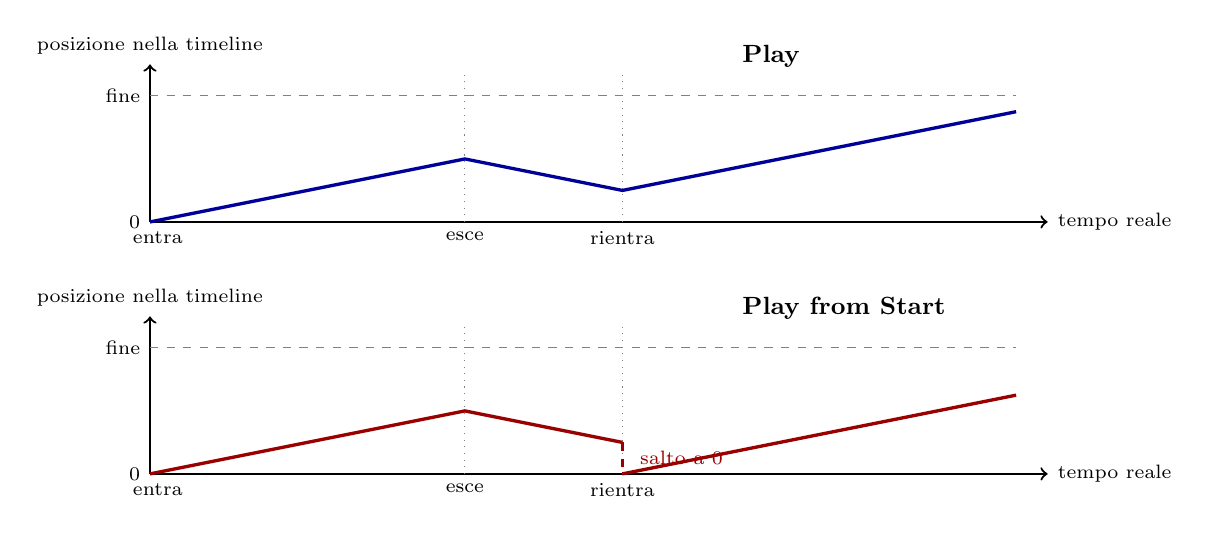
\begin{tikzpicture}[font=\footnotesize, x=1.0cm, y=1.0cm]
  \foreach \y/\titolo in {0/Play, -3.2/Play from Start} {
    \begin{scope}[yshift=\y cm]
      \draw[->, thick] (0,0) -- (11.4,0) node[right, font=\scriptsize]{tempo reale};
      \draw[->, thick] (0,0) -- (0,2.0) node[above, font=\scriptsize]{posizione nella
        timeline};
      \draw[gray, dashed] (0,1.6) -- (11,1.6);
      \node[font=\scriptsize, left] at (0,1.6) {fine};
      \node[font=\scriptsize, left] at (0,0) {0};
      \node[font=\small\bfseries, anchor=west] at (7.4,2.1) {\titolo};
      \draw[gray, dotted] (4,0) -- (4,1.9);
      \draw[gray, dotted] (6,0) -- (6,1.9);
      \node[font=\scriptsize, below] at (0.1,0) {entra};
      \node[font=\scriptsize, below] at (4,0) {esce};
      \node[font=\scriptsize, below] at (6,0) {rientra};
    \end{scope}
  }
  % Play
  \draw[very thick, blue!60!black] (0,0) -- (4,0.8) -- (6,0.4) -- (11,1.4);
  % Play from start
  \draw[very thick, red!60!black] (0,-3.2) -- (4,-2.4) -- (6,-2.8);
  \draw[very thick, red!60!black, dashed] (6,-2.8) -- (6,-3.2);
  \draw[very thick, red!60!black] (6,-3.2) -- (11,-2.2);
  \node[font=\scriptsize, red!60!black, anchor=west] at (6.1,-3.0) {salto a 0};
\end{tikzpicture}
\caption{Entrare, uscire a metà e rientrare prima che la timeline sia tornata a 0. Con
Play (in alto) la timeline riprende da dove si trova; con Play from Start (in basso)
salta all'inizio, e l'oggetto fa uno scatto. Schema ricostruito come integrazione alla
risposta del docente.}
\label{ue7:fig:play}
\end{figure}

% ---------------------------------------------------------------------
\section{Gli attivabili: la classe BP\_Activable}
\label{ue7:sec:activable}

``Adesso andiamo a fare una cosa bellina.'' Il pulsante si muove, ma non fa ancora
niente. Prima di creare la luce, ``prima, importante'', serve una \textbf{tipologia di
actor}: quella degli \textbf{attivabili}, ``quelli che per noi saranno gli attivabili''.

\paragraph{La classe base.} Un nuovo Blueprint Class di tipo Actor: il docente lo chiama
BP\_Activable1, qui è semplicemente \textbf{BP\_Activable}. ``Che succede qui all'interno? Ci serve solo
questo'': con la sola creazione ``abbiamo intanto definito una tipologia di actor''.
Dentro, due \textbf{Custom Event}:
\begin{itemize}
  \item \textbf{Activation}, collegato a un Print String ``attivato'';
  \item \textbf{Deactivation}, collegato a un Print String ``deattivato'' (cioè
        disattivato).
\end{itemize}
``Questi due eventi saranno collegati all'attivare qualcosa o disattivare qualcosa.'' Le
due stampe sono provvisorie: servono a vedere che il collegamento funziona, e poi a
capire come i figli possono \emph{sovrascrivere} gli eventi del padre
(sezione~\ref{ue7:sec:override}).

\paragraph{La domanda.} ``Quando è che io lo devo chiamare? E soprattutto, come faccio a
fargli dire: ehi, bottone, guarda che devi attivare questo esatto elemento?'' La risposta
è una variabile nel bottone, ed è il cuore della lezione.

% ---------------------------------------------------------------------
\section{Il bottone e la lista degli attivabili}
\label{ue7:sec:array}

\paragraph{Una variabile di tipo BP\_Activable.} Nel Blueprint del bottone si crea una
variabile, \textbf{ActivableItems}, e se ne cambia il tipo. ``Questo è molto
interessante, ragazzi: possiamo creare una variabile del tipo di quell'asset che abbiamo
appena creato'': il tipo è \textbf{BP\_Activable}, nella forma \emph{Object Reference}.
Una variabile così non contiene un numero o un testo, ma un \textbf{riferimento} a un
attivabile presente nel livello.

\paragraph{Pubblica.} ``Facciamola \textbf{pubblica}, e si fa con questo
\textbf{occhietto}'' accanto alla variabile. Il docente mette nel livello un
BP\_Activable e seleziona il pulsante: nei Details, in \emph{Default}, ``è apparso
Activable Items''. ``Vuol dire che questa variabile è modificabile dai Details del nostro
editor'', e quindi ``ci permette di avere interazioni dirette con la viewport,
l'ambiente di gioco'': ogni copia del pulsante nel livello può avere i suoi oggetti da
attivare.

\paragraph{Un array.} ``All'inizio di lezione abbiamo parlato degli array'': il pulsante
non deve attivare un oggetto solo, ``ma una moltitudine di oggetti''. Si cambia quindi
non la \emph{tipologia} della variabile, ma la sua \textbf{costituzione} (``cerchiamo di
dividerli'', precisa il docente): accanto al \emph{Variable Type} c'è un'icona (``questo
cilindro, vabbè, un'ellisse'') con una freccetta, e il menù offre \textbf{Single},
\textbf{Array}, \textbf{Set} e \textbf{Map} (tabella~\ref{ue7:tab:contenitori}). Si sceglie
Array, e l'icona della variabile cambia: ``diventa una matrice'', una griglia di
quadratini. ``Adesso abbiamo una variabile array di tipologia BP\_Activable.''

\begin{table}[htbp]
\centering
\small
\begin{tabular}{@{}p{2.4cm}p{5.8cm}p{5.8cm}@{}}
\toprule
\textbf{Costituzione} & \textbf{Che cosa contiene} & \textbf{Esempio} \\
\midrule
Single & un valore solo (la ``scatola'') & la referenza a una sola luce \\
Array & una lista ordinata di valori dello stesso tipo, con indice da 0; ammette
doppioni & gli oggetti attivati dal pulsante (ActivableItems) \\
Set & un insieme di valori unici, senza ordine e senza indice & i nomi degli oggetti
già raccolti \\
Map & coppie chiave--valore, con chiavi uniche & il nome di un'arma e le sue
munizioni \\
\bottomrule
\end{tabular}
\caption{Le quattro costituzioni di una variabile, dal menù accanto al Variable Type.
La lezione usa Single e Array; le descrizioni di Set e Map seguono Romero e Sewell
(capitolo 13).}
\label{ue7:tab:contenitori}
\end{table}

\paragraph{Quando chiamare gli attivabili.} ``Vogliamo che quando il nostro bel bottone
finisce di fare il suo percorso, e si schiaccia'', partano le attivazioni: si usa
l'uscita \textbf{Finished} della timeline. Ma Finished scatta sia alla fine della
discesa sia alla fine della risalita (dopo il Reverse), quindi bisogna sapere ``che
direzione è''. ``Vi ricordate che abbiamo usato lo Switch l'altra volta sulla
Direction?'' Dal pin \textbf{Direction} si crea uno \textbf{Switch on
ETimelineDirection}, collegato al Finished:
\begin{itemize}
  \item \textbf{Forward}: la timeline è andata avanti, il pulsante è schiacciato,
        quindi \textbf{attiva};
  \item \textbf{Backward}: la timeline è tornata indietro, il pulsante è tornato
        ``alla sua posizione di prima'', quindi \textbf{disattiva}.
\end{itemize}

\paragraph{Il For Each Loop.} ``Abbiamo già visto il For Loop. Questo è il \textbf{For
Each Loop}.'' Si prende un \emph{Get} di ActivableItems e se ne tira fuori il ciclo:
``questa esecuzione verrà fatta per ogni elemento dell'array che abbiamo inserito qua
dentro''; ``abbiamo cinque elementi dentro l'array, verrà fatto cinque volte''. Il nodo ha
due uscite di dati: l'\textbf{Array Element}, ``il singolo elemento che ha preso in
considerazione nel momento preciso del ciclo'', e l'\textbf{Array Index}. Dall'Array
Element, che è di tipo BP\_Activable, si può chiamare direttamente l'evento
\textbf{Activation}, collegato al \textbf{Loop Body}. Per il ramo Backward ``i primi due
li prendete, li copiate, li mettete sotto'': stesso Get, stesso For Each Loop, ma con
\textbf{Deactivation} (figura~\ref{ue7:fig:foreach}).

\begin{figure}[htbp]
\centering
\begin{tikzpicture}[font=\footnotesize,
  ue7node/.style={draw, thick, rounded corners=4pt, align=center, fill=gray!8,
                  minimum height=0.8cm, text width=2.0cm},
  ue7var/.style={ue7node, fill=blue!10, rounded corners=8pt},
  ue7ev/.style={ue7node, fill=red!12},
  ue7exec/.style={-{Stealth[length=2.5mm]}, very thick, black!80},
  ue7data/.style={-{Stealth[length=2mm]}, thick, violet!60!black}]
  \node[ue7node, fill=red!8, text width=1.8cm, minimum height=1.8cm] (tl) at (0,0)
    {\textbf{Timeline}\\PushButton};
  \node[ue7node, text width=2.1cm] (sw) at (3.3,0) {\textbf{Switch on
    ETimelineDirection}};
  \node[ue7node, text width=1.9cm] (fe1) at (6.7,1.4) {\textbf{For Each Loop}};
  \node[ue7node, text width=1.9cm] (fe2) at (6.7,-1.4) {\textbf{For Each Loop}};
  \node[ue7var, text width=2.4cm] (g1) at (6.7,3.1) {\textbf{Get}\\ActivableItems};
  \node[ue7var, text width=2.4cm] (g2) at (6.7,-3.1) {\textbf{Get}\\ActivableItems};
  \node[ue7ev, text width=2.1cm] (a) at (10.4,1.4) {Array Element $\rightarrow$
    \textbf{Activation}};
  \node[ue7ev, text width=2.1cm] (d) at (10.4,-1.4) {Array Element $\rightarrow$
    \textbf{Deactivation}};
  \draw[ue7exec] ([yshift=0.4cm]tl.east) -- node[above, font=\scriptsize]{Finished}
    ([yshift=0.4cm]sw.west);
  \draw[ue7data] ([yshift=-0.4cm]tl.east) -- node[below, font=\scriptsize]{Direction}
    ([yshift=-0.4cm]sw.west);
  \draw[ue7exec] (sw.north) |- node[pos=0.25, left, font=\scriptsize]{Forward} (fe1.west);
  \draw[ue7exec] (sw.south) |- node[pos=0.25, left, font=\scriptsize]{Backward} (fe2.west);
  \draw[ue7data] (g1) -- node[right, font=\scriptsize]{Array} (fe1);
  \draw[ue7data] (g2) -- node[right, font=\scriptsize]{Array} (fe2);
  \draw[ue7exec] (fe1) -- node[above, font=\scriptsize]{Loop Body} (a);
  \draw[ue7exec] (fe2) -- node[below, font=\scriptsize]{Loop Body} (d);
\end{tikzpicture}
\caption{Il pulsante chiama gli attivabili. Alla fine della timeline, lo Switch sulla
Direction sceglie il ramo: in avanti (pulsante schiacciato) un For Each Loop chiama
Activation su ogni elemento di ActivableItems; all'indietro (pulsante rilasciato) un
secondo ciclo chiama Deactivation. Schema ricostruito.}
\label{ue7:fig:foreach}
\end{figure}

\paragraph{Riempire l'array.} ``Ci manca ancora una piccola particolarità'': la variabile
è pubblica perché gli oggetti da attivare si scelgono \emph{nel livello}. Si clicca sul
pulsante nella scena, e in \emph{Default} c'è Activable Items: con il \textbf{+} si
aggiungono gli elementi, ``tutti quelli che volete''. Prima, però, un'avvertenza: ``in
informatica si parte non da uno, ma da \textbf{zero}''; ``l'indice 0 è il primo
indice''. Il primo elemento dell'array è l'elemento 0. Per assegnargli un oggetto ci sono
due modi:
\begin{itemize}
  \item il \textbf{menù a tendina}, che elenca ``tutti gli oggetti che puoi ficcarci
        dentro questo array'', cioè tutti i BP\_Activable presenti nel livello, ``perché
        giustamente è quello'';
  \item il \textbf{contagocce} (\emph{pick actor from scene}), ``proprio come su
        Photoshop'': si clicca sull'icona e si passa sopra gli oggetti della scena;
        sugli oggetti di un altro tipo l'editor avvisa che ``non è compatibile'', sul
        BP\_Activable invece ``è compatibile, ci può entrare dentro''. Un clic, ``ecco che
        è apparso''.
\end{itemize}
In Play, sul pulsante: ``attivato''; si scende: ``disattivato''. ``Vi funziona?''

\paragraph{I problemi.} A una studentessa, sul pulsante non compare la voce dell'array:
``basta che vai dove sono le variabili: c'è l'occhietto. Hai l'occhietto chiuso?''. Si
apre l'occhio, si compila (``se no non va''), e la voce compare. Poi bisogna
\textbf{mettere in scena} l'attivabile, se non c'è, e collegarlo con il contagocce
(``c'è la freccettina, c'è questo mouse con dei riquadri, e subito dopo c'è il
contagocce''). ``Sì, funziona. Ottimo.''

``Quindi, ragazzi, adesso abbiamo creato il funzionamento base'', cioè ``la relazione
tra pulsante e oggetto''. L'oggetto non ha ancora particolari funzionalità, ``se non
stampare due frasi'', ``tuttavia la base ce l'abbiamo''.

\paragraph{Approfondimento: la comunicazione diretta.} Quello costruito è ciò che Romero
e Sewell (capitolo 4) chiamano \textbf{Direct Blueprint Communication}: un Blueprint
tiene una variabile referenza a un altro actor, e la usa come \emph{Target} per
chiamarne le funzioni e gli eventi. Il loro esempio è sorprendentemente vicino a quello
della lezione: un \emph{BP\_LightSwitch} con una variabile di tipo Point Light, resa
\textbf{Instance Editable} (l'``occhietto'' del docente: ogni istanza nel livello può
avere un valore diverso), che a ogni overlap del giocatore accende o spegne una lampada
scelta nei Details dal menù a tendina. La lezione fa un passo in più in due direzioni:
la referenza è un \emph{array}, quindi un pulsante comanda molti oggetti; e il tipo è una
classe \emph{parent} scritta da noi, quindi il pulsante non sa e non deve sapere se
l'oggetto è una luce o una piattaforma. Il libro aggiunge un consiglio che vale anche
qui: prima di usare una referenza, controllarla con \textbf{Is Valid}, perché un elemento
dell'array lasciato vuoto nei Details (il \textbf{+} premuto senza scegliere niente)
produrrebbe l'errore ``Accessed None'' visto a inizio lezione. Lo stesso capitolo 13
mostra il For Each Loop proprio su un array di Point Light, ``le lampade di una
stanza''.

% ---------------------------------------------------------------------
\section{Il figlio: BP\_ActivableLight e i due Begin Play}
\label{ue7:sec:child}

``A questo punto andiamo a evolvere questo attivabile in una luce che si accende e si
spegne.'' Ma, attenzione: ``non andiamo a creare un nuovo Blueprint, ma andiamo a creare
un \textbf{figlio} di questo Blueprint, perché vogliamo che condivida la particolarità di
avere le fasi di attivazione e disattivazione''.

\paragraph{Create Child Blueprint Class.} Tasto destro su BP\_Activable nel Content
Browser, \textbf{Create Child Blueprint Class} (``lo trovate tutto sopra''). Unreal
propone un nome con il suffisso \emph{Child}; il docente lo chiama
\textbf{BP\_ActivableLight}. Aprendolo, in alto a destra nell'editor si legge già il
\textbf{Parent class}: ``guarda, questo è il parent, questo è il suo papà; deriva da
questo''. Una studentessa non trova il comando: va fatto con il tasto destro proprio su
BP\_Activable, non sulla pedana.

\paragraph{Event BeginPlay e Parent: BeginPlay.} Aprendo il figlio, al docente compaiono
nel grafo due nodi: \textbf{Event BeginPlay} e, collegato a esso, un nodo
\textbf{Parent: BeginPlay}. Agli studenti no: il docente aveva cancellato il Begin Play
dal parent. La prova: nel parent si rimette un \textbf{Event BeginPlay} (con un Print
String, ``così si vede bene''), e il figlio creato dopo li mostra entrambi. Il
significato: ``io eseguirò il tuo Event BeginPlay assieme all'Event BeginPlay del mio
papà''. ``Va a eseguire in sostanza due Begin Play.''

\paragraph{La dimostrazione.} Nel figlio il Begin Play non contiene niente, a parte la
chiamata al parent; eppure, in Play, la stampa del parent compare. ``Questo è il child.
Qua dentro non c'è un Print String, non c'è niente. Ma lui andrà a fare il Begin Play
del suo papà.'' Se si \textbf{stacca} il nodo Parent: BeginPlay, ``non mi stampa più
niente''. Lo stesso varrebbe per ogni altro evento: ``se dovessimo fare un Event Begin
Overlap, avremmo la stessa identica cosa'', cioè la domanda ``vuoi che ti esegua anche
quello del tuo papà? Sì o no?''. Il nodo si può anche cancellare: ``questo era per
spiegare la \textbf{condivisione degli eventi}''.

\paragraph{Approfondimento: estendere o sostituire.} Il nodo \emph{Parent: BeginPlay} è
la chiave per capire l'override. Quando un child definisce un evento che esiste già nel
parent, la sua versione \emph{sostituisce} quella del parent; il nodo
\emph{Parent:~\ldots}, collegato al filo di esecuzione, la richiama in un punto preciso.
Collegato all'inizio, il child fa prima ciò che fa il parent e poi aggiunge il suo
(\emph{estende}); collegato alla fine, aggiunge prima il suo; scollegato o cancellato, il
child fa solo il suo (\emph{sostituisce}). Unreal lo crea in automatico quando il parent
ha già quell'evento, come gentile promemoria; se manca, si aggiunge con il tasto destro
sul nodo dell'evento, \textbf{Add Call to Parent Function}. Servirà nella
sezione~\ref{ue7:sec:parent}.

% ---------------------------------------------------------------------
\section{La luce: la Point Light}
\label{ue7:sec:luce}

``Andiamo a mettere questa bella lucina.'' Il docente illumina un po' il suo asset ``perché
così non si può vedere'', e aggiunge al figlio un componente \textbf{Point Light}, la luce
puntiforme che illumina in tutte le direzioni: ``la potete vedere che si è creato un
reticolo''. I parametri principali, uno alla volta, in una piccola finestra di prova:
\begin{itemize}
  \item \textbf{Intensity}: ``l'intensità della luce: aumenta, diminuisce'';
  \item \textbf{Attenuation Radius}: il raggio disegnato attorno alla luce, ``quanto si
        espande''; se lo si allarga, il muro vicino viene illuminato;
  \item \textbf{Source Radius}: ``il raggio della sua sorgente'', il ``pallino'' che si
        vede al centro quando si guarda una luce;
  \item \textbf{Soft Source Radius} e \textbf{Source Length} (``la lente, volendo, si
        evolve in verticalità: una specie di lampione tutto strano''), ``una cosa un po'
        più particolare'';
  \item \textbf{Light Color}: con la ruota dei colori, il cursore del chiaro e scuro e
        quello della ``tendenza al bianco'' (la saturazione). Il docente la fa
        \textbf{blu}, ``per differenziarla dall'altra''.
\end{itemize}
L'intensità finale è \textbf{20.000} (il docente dice prima ``200.000'', poi si
corregge: ``20.000, scusate''). ``Questo era semplicemente un piccolo cenno sulle
luci.''

\paragraph{Approfondimento: unità e mobilità delle luci.} In Unreal Engine 5 l'intensità
di una Point Light si misura di solito in \textbf{candele} (o in lumen), e il valore
predefinito di una luce nuova è basso; 20.000 nella vecchia unità adimensionale
(\emph{Unitless}) è invece una luce molto forte, e il numero giusto dipende dall'unità
impostata nel campo \emph{Intensity Units} e dall'esposizione della camera. C'è poi una
condizione per poter cambiare una luce \emph{mentre il gioco gira}: la sua
\textbf{Mobility} deve essere \emph{Movable} (o \emph{Stationary} per intensità e
colore), non \emph{Static}, perché le luci statiche vengono ``cotte'' nelle lightmap e
non esistono più come luci a runtime. Romero e Sewell lo fanno notare nell'esempio del
loro interruttore: la lampada va resa Movable. Con Lumen, il sistema di illuminazione
dinamica predefinito di Unreal Engine 5, le luci sono in genere già Movable.

% ---------------------------------------------------------------------
\section{Salvare l'intensità e sovrascrivere gli eventi}
\label{ue7:sec:override}

``Ci serve, per mettere i due stadi di activation e deactivation, prima di tutto'' un
passaggio nel \textbf{Begin Play}. La luce deve partire spenta, e accendersi poi con
l'intensità scelta nell'editor (20.000). Ma se all'inizio la si spegne, quel numero
andrebbe perso.

\paragraph{IntensityStart.} ``Vi ricordo che tutte le cose che vedete'' nei Details
``sono tutte modificabili, sono tutte richiamabili.'' Dal componente Point Light si tira
fuori \textbf{Get Intensity} (``stiamo prendendo l'intensità attuale'') nel Begin Play,
``all'inizio, quando il frame esiste'', e con \textbf{Promote to Variable} si salva in
una nuova variabile, \textbf{IntensityStart}: ``una variabile di \textbf{appoggio}'',
che serve solo a ricordare il valore da riproporre quando la luce si accenderà. ``Non
serve il Parent: BeginPlay'', aggiunge il docente, ``perché tanto nel parent non facciamo
niente.''

\paragraph{Il problema delle stampe.} Se ora si chiamano gli eventi Activation e
Deactivation sulla luce, la luce ``rimane accesa, è normale'', e in più il figlio
``condividerà il fatto'' di stampare ``attivato'' e ``deattivato'': ha ereditato gli
eventi del padre così come sono. ``Noi non vogliamo questo: noi vogliamo semplicemente
che la luce si spenga.''

\paragraph{L'override.} ``Come facciamo a sovrascrivere questo evento?'' Nel pannello My
Blueprint, accanto a \emph{Functions}, c'è il menù \textbf{Override}: elenca gli eventi
e le funzioni che si possono ridefinire, quelli di Actor (``ActorBeginCursorOver'',
``BeginPlay'', ``Reset'' e così via) e, in fondo, \textbf{Activation} e
\textbf{Deactivation}, ereditati da BP\_Activable. Scegliendoli, compaiono nel grafo del
figlio. ``Che vuol dire override? Vuol dire che stiamo \textbf{sovrascrivendo}'' gli
eventi. Prova: in Play, con i due eventi vuoti, ``non mi fa più niente. È giusto così'':
la versione del figlio ha preso il posto di quella del padre. ``Possiamo sovrascrivere
vari eventi all'interno dei child, in modo tale da facilitarci la differenziazione dei
comportamenti.''

\paragraph{Accendere e spegnere.}
\begin{itemize}
  \item Su \textbf{Activation}: dalla Point Light, \textbf{Set Intensity} (``invece di
        get, set''), con \emph{New Intensity} collegato a \textbf{IntensityStart}.
  \item Su \textbf{Deactivation}: Set Intensity a \textbf{0}.
\end{itemize}
Il Target dei due nodi è la Point Light, ``perché stanno qui'', nel figlio.

\paragraph{L'ordine nel Begin Play.} Resta da spegnere la luce all'avvio: nel Begin Play,
``subito dopo il salvarsi la variabile'', si chiama \textbf{Deactivation}. ``Perché non lo
facciamo prima? Perché se facessimo Deactivation prima, il valore che si salverebbe è
zero'' (figura~\ref{ue7:fig:luce}). In Play: la luce, accesa nell'editor, ``si spegne
perché l'ho disattivata''; si sale sul pulsante, ``adesso si accende''. ``Abbiamo fatto il
nostro bottone con una pre-impostazione tra trigger e triggerato.''

\begin{figure}[htbp]
\centering
\begin{tikzpicture}[font=\footnotesize,
  ue7node/.style={draw, thick, rounded corners=4pt, align=center, fill=gray!8,
                  minimum height=0.8cm, text width=2.0cm},
  ue7var/.style={ue7node, fill=blue!10, rounded corners=8pt},
  ue7ev/.style={ue7node, fill=red!12},
  ue7ov/.style={ue7node, fill=orange!18},
  ue7exec/.style={-{Stealth[length=2.5mm]}, very thick, black!80},
  ue7data/.style={-{Stealth[length=2mm]}, thick, violet!60!black}]
  % begin play
  \node[ue7ev, text width=1.9cm] (bp) at (0,2.2) {\textbf{Event BeginPlay}};
  \node[ue7node, text width=2.1cm] (gi) at (3.6,3.7) {Point Light $\rightarrow$
    \textbf{Get Intensity}};
  \node[ue7var, text width=2.0cm] (set) at (3.6,2.2) {\textbf{Set}\\IntensityStart};
  \node[ue7node, text width=2.0cm] (de) at (7.0,2.2) {\textbf{Deactivation}\\(chiamata)};
  \draw[ue7exec] (bp) -- (set);
  \draw[ue7exec] (set) -- (de);
  \draw[ue7data] (gi) -- (set);
  \node[font=\scriptsize, align=left, anchor=west] at (8.3,2.2) {prima si salva,\\poi
    si spegne};
  % override
  \node[ue7ov, text width=2.0cm] (ac) at (0,0) {\textbf{Activation}\\(override)};
  \node[ue7node, text width=2.3cm] (si1) at (3.6,0) {Point Light $\rightarrow$
    \textbf{Set Intensity}};
  \node[ue7var, text width=1.8cm] (gis) at (7.6,0) {\textbf{Get}\\IntensityStart};
  \draw[ue7exec] (ac) -- (si1);
  \draw[ue7data] (gis) -- node[above, font=\scriptsize]{New Intensity} (si1);
  \node[ue7ov, text width=2.0cm] (dc) at (0,-1.8) {\textbf{Deactivation}\\(override)};
  \node[ue7node, text width=2.3cm] (si2) at (3.6,-1.8) {Point Light $\rightarrow$
    \textbf{Set Intensity}\\New Intensity 0};
  \draw[ue7exec] (dc) -- (si2);
\end{tikzpicture}
\caption{Il grafo di BP\_ActivableLight. Nel Begin Play l'intensità scelta nell'editor
viene salvata in IntensityStart e solo dopo la luce viene spenta; i due eventi ereditati
da BP\_Activable sono sovrascritti (override) e accendono o spengono la Point Light.
Schema ricostruito.}
\label{ue7:fig:luce}
\end{figure}

\paragraph{I problemi.}
\begin{itemize}
  \item A uno studente la luce resta accesa, e in più compaiono ancora le scritte
        ``attivato'' e ``deattivato''. Il docente ripete la sequenza; lo studente ritrova
        l'errore da solo: ``avevo collegato per sbaglio IntensityStart pure a quello
        sotto'', cioè anche al Set Intensity della Deactivation, che quindi riaccendeva la
        luce invece di spegnerla.
  \item A un'altra studentessa, quando preme Play, ``non si vede più la luce'': è
        giusto, la luce parte spenta. Ma poi non si accende, e appare solo la stampa.
        Causa: il pulsante nel livello è ancora collegato al BP\_Activable di prova, non
        alla luce. ``Prendi il contagocce e clicca su BP\_ActivableLight.''
\end{itemize}

\paragraph{Approfondimento: gli eventi di BP\_Activable come contratto.} Il risultato di
queste sezioni è un piccolo esempio di \emph{polimorfismo}, il concetto che Romero e
Sewell illustrano con le armi che ridefiniscono \emph{Fire}. Il pulsante chiama
Activation su ogni elemento dell'array senza sapere che cosa ci sia dentro; ogni oggetto
risponde con la propria versione dell'evento. Per aggiungere al gioco un nuovo oggetto
attivabile (una porta, un ventilatore, una trappola) non serve toccare il pulsante:
basta un nuovo child di BP\_Activable che sovrascriva i due eventi. Il parent fa da
\emph{contratto}: ``chi è attivabile sa rispondere ad Activation e Deactivation''. È anche
il motivo per cui conviene lasciare il parent quasi vuoto: le due stampe di prova sono
utili oggi, ma in un progetto vero un evento del parent che stampa qualcosa finirebbe
per stampare in ogni figlio che non lo sovrascrive.

% ---------------------------------------------------------------------
\section{La pausa e il suono della piattaforma}
\label{ue7:sec:pausa}

``Ragazzi, sono le 5 e mezza.'' Il programma della seconda parte: la piattaforma che si
attiva con il pulsante, ``magari un po' come esercizio'', e ``un altro metodo, che è
quello degli \textbf{event dispatcher}''. ``Ci vediamo al solito orario, 17:55, 18.''

Durante la pausa il docente mantiene la promessa fatta a inizio lezione, e completa con
lo studente rimasto indietro l'\textbf{audio della piattaforma} della sesta lezione, in
condivisione dello schermo. È un ripasso utile, perché raccoglie in un unico passaggio
l'ordine corretto dei nodi.
\begin{enumerate}
  \item Il file audio è già importato e impostato (il docente lo verifica aprendolo).
  \item In fondo al grafo, dopo l'Update della timeline, si toglie il Print String di
        prova e si aggiunge un \textbf{Do Once}.
  \item Dopo il Do Once, \textbf{Spawn Sound at Location}, con la \emph{Location} presa
        da \textbf{Get Actor Location} (``spazio vuoto, tasto destro''), collegata al pin
        arancione e non a quello azzurro, e il suono della piattaforma nel campo
        \emph{Sound}.
  \item Dal \emph{Return Value} (``quel pallino blu''), \textbf{Promote to Variable}:
        \textbf{SoundPlatform}.
  \item Solo ora, dal pin \textbf{Direction} della timeline, lo \textbf{Switch on
        ETimelineDirection}, collegato dopo il Set della variabile (``portalo tutto in
        avanti, oltre quello''): su \textbf{Forward}, SoundPlatform $\rightarrow$
        \textbf{Set Pitch Multiplier} a 1; su \textbf{Backward}, una copia con pitch
        \textbf{0,4}.
  \item Sul \textbf{Finished}: SoundPlatform $\rightarrow$ \textbf{Stop}, e dallo Stop
        il \textbf{Reset} del Do Once.
\end{enumerate}
``Si sente l'audio. A posto, perfetto.'' La registrazione della pausa, per il resto, è
coperta dai soliti blocchi senza senso della trascrizione automatica.

% ---------------------------------------------------------------------
\section{La correzione del pitch}
\label{ue7:sec:pitch}

Alla ripresa, ``una piccola cosa per Filippo'', che a inizio lezione aveva segnalato il
bug del suono. Il problema: lo Switch sulla Direction viene eseguito solo dopo lo spawn
del suono, che grazie al Do Once avviene una volta sola, all'inizio del movimento. Se il
giocatore scende dalla piattaforma mentre sta ancora salendo, la timeline va in Reverse,
ma nessuno rimette il pitch: ``partiva e lo faceva solo una volta, quindi non si trova
mai il pitch''.

La correzione è semplice: ``il pitch del suono va settato in automatico sia se va
backwards, sia se esce dal volume''. Sull'\textbf{End Overlap}, prima del
\textbf{Reverse}, si aggiunge SoundPlatform $\rightarrow$ \textbf{Set Pitch Multiplier}
a \textbf{0,4}: ``nel momento esatto in cui esce dal volume, settiamo il pitch a 0,4'',
``anche se in mezzo alla piattaforma mi lancio''. ``E siamo tranquilli.''

\paragraph{Approfondimento: lo stesso errore, di nuovo.} Il nuovo Set Pitch Multiplier
ha lo stesso rischio dell'errore di inizio lezione: se il giocatore entra ed esce dalla
box prima che la timeline abbia prodotto il primo Update, SoundPlatform è ancora vuota,
e l'End Overlap la usa. In pratica capita di rado, ma una macro \textbf{Is Valid} sulla
variabile, prima del Set, lo esclude del tutto. Più in generale, un suono il cui pitch
deve seguire la direzione del movimento si gestisce meglio leggendo la Direction della
timeline a ogni Update (o, ancora meglio, chiamando Set Pitch Multiplier ogni volta che
si chiamano Play o Reverse), invece che una volta sola all'inizio.

% ---------------------------------------------------------------------
\section{Un altro metodo: gli event dispatcher}
\label{ue7:sec:dispatcher}

``Allora, ragazzi, eravamo rimasti con il nostro bottoncino che ci dava la possibilità di
accendere e spegnere una luce. Possiamo usare questo metodo, però volendo potremmo anche
vedere un altro modo'': gli \textbf{event dispatcher}. Si trovano nel pannello My
Blueprint del bottone, sotto \emph{Variables}, nella sezione \textbf{Event Dispatchers}.

\paragraph{Che cosa sono.} ``Gli event dispatcher, a differenza dei custom event, ci
permettono di \textbf{bindare} vari eventi tra di loro''; ``bindare sta per
collegare''. L'esempio del docente: tre custom event, A, B e C. Con un event dispatcher
si possono legare A, B e C tutti insieme a un altro evento, oppure solo A e C: ``a un
evento di salto succede che si salta; voglio che mi faccia, assieme al salto, A e C''.
Così si tengono separati, per esempio, un controllo e uno sparo, e li si fa partire
insieme quando serve: ``guarda che quando salta, bindami questo evento allo sparo o al
controllo''. ``È un modo un po' più ordinato per fare le cose.'' Lo scopo, oggi, resta lo
stesso: accendere e spegnere la luce con il bottone.

\paragraph{Il dispatcher e il suo parametro.} Con il \textbf{+} accanto a Event
Dispatchers si crea \textbf{OnCheckStatus} (nella trascrizione ``on share status'' e
``check status''; il nome esatto non è del tutto sicuro, ma è quello che il docente usa
nel resto della spiegazione). Come i custom event, anche un dispatcher può avere
\emph{input}: nei Details, con il \textbf{+} della sezione \emph{Inputs}, si aggiunge un
\emph{New Parameter}, rinominato \textbf{IsActive}. Il tipo proposto di base è proprio
il \textbf{Boolean}, ``e va benissimo così'': vero vuol dire che il bottone è attivato,
falso che è disattivato.

\paragraph{A parti invertite.} ``Ma in questo caso andremo a fare una cosa differente.
Invece che il bottone chiami la luce, sarà la luce a controllare lo stato del bottone:
a parti inverse.'' Il pulsante non avrà più bisogno di sapere quali oggetti attivare;
saranno gli oggetti ad \emph{ascoltare} il pulsante. Il docente, per un attimo, stacca
Activation e Deactivation dal resto; poi ci ripensa: ``li useremo comunque in ogni
caso, perdonate''.

% ---------------------------------------------------------------------
\section{La luce si mette in ascolto: Get Actor Of Class e Bind Event}
\label{ue7:sec:bind}

Nel \textbf{Begin Play} di BP\_ActivableLight (dopo il salvataggio dell'intensità) la luce
deve trovare il pulsante e ``attaccarsi'' al suo dispatcher.

\paragraph{Get Actor Of Class.} ``Andiamo a ricercare in tutto il gioco, cioè in tutto lo
spazio di gioco, un attore in particolare.'' Il nodo \textbf{Get Actor Of Class} riceve
una \emph{Actor Class}, qui \textbf{BP\_Button}, e restituisce un actor di quella classe
presente nel livello.

\paragraph{Bind Event.} Dal valore restituito si tira fuori \textbf{Bind Event to
OnCheckStatus}. Il nodo appena creato dà errore: ``è normale, ho fatto compilare prima
del tempo''. Il suo significato, ``letteralmente'': ``attacca un evento''. Quale? Dal pin
rosso \emph{Event} del nodo si tira fuori un filo e si crea un \textbf{Custom Event},
chiamato \textbf{CheckStatusEvent}. ``Guardate la cosa interessante'': il nuovo evento ha
\emph{già} un'uscita \textbf{IsActive}. Un custom event normale nasce vuoto; questo nasce
con la stessa \emph{firma} del dispatcher, ``perché comunque sono in comunicazione'':
``nel check status ci sono questi parametri, che servono alla comunicazione'', e il nodo
li riporta ``nell'evento che tu mi costruisci''. ``Sono due eventi in comunicazione.''

\paragraph{La decisione.} Dentro CheckStatusEvent, ``letteralmente'' un \textbf{Branch}
sul booleano IsActive: se è vero, \textbf{Activation}; se è falso, \textbf{Deactivation}.
Gli eventi sovrascritti della luce restano quelli di prima; cambia solo chi li fa
partire (figura~\ref{ue7:fig:dispatcher}).

% ---------------------------------------------------------------------
\section{Il bottone chiama: Call}
\label{ue7:sec:call}

``La cosa è che il controllo sta dalla parte della nostra carissima luce. Ma come
facciamo a chiamarlo?'' Nel bottone, dopo lo Switch on ETimelineDirection (``subito
dopo, oppure in sostituzione; in questo caso facciamo subito dopo''), si trascina
OnCheckStatus nel grafo. Il menù offre \textbf{Call}, \textbf{Bind}, \textbf{Unbind},
\textbf{Unbind All}, \textbf{Event} e \textbf{Assign}. Si sceglie \textbf{Call}:
``quando succederà questo evento della timeline, che andrà avanti o indietro, chiamami
questo evento e tutti quegli eventi che sono bindati''.
\begin{itemize}
  \item Sul ramo \textbf{Forward}, dopo il For Each Loop delle attivazioni: Call
        OnCheckStatus con \textbf{IsActive vero} (``se è forward, vuol dire che è
        attivo'').
  \item Sul ramo \textbf{Backward}: Call OnCheckStatus con \textbf{IsActive falso}.
\end{itemize}

\paragraph{La prova.} Per dimostrare che il nuovo metodo funziona da solo, il docente
``svuota'' il bottone dalle chiamate dirette: stacca i For Each Loop, lascia collegate
``solamente le due Call, e basta''; nell'array della luce non serve più nulla, ``la
referenza non ci serve''. In Play la luce si accende e si spegne comunque, ``perché sto
eseguendo un check status quando il bottone viene premuto, e lui si ricorda che
all'inizio gli ho collegato quest'altro evento''. ``È come se lo tenesse in memoria.''
``È come dire un \textbf{raggruppamento di eventi}.'' E un'osservazione in risposta a una
perplessità: il Bind è nel Begin Play, ma l'evento non scatta solo nel Begin Play; nel
Begin Play si \emph{stabilisce il legame}, che poi vale ``ogni volta che lo usi''.

\begin{figure}[htbp]
\centering
\begin{tikzpicture}[font=\footnotesize,
  ue7bp/.style={draw, very thick, rounded corners=6pt, inner sep=6pt},
  ue7node/.style={draw, thick, rounded corners=4pt, align=center, fill=gray!8,
                  minimum height=0.8cm, text width=2.1cm},
  ue7ev/.style={ue7node, fill=red!12},
  ue7disp/.style={ue7node, fill=yellow!35},
  ue7exec/.style={-{Stealth[length=2.5mm]}, very thick, black!80},
  ue7link/.style={-{Stealth[length=2.5mm]}, very thick, dashed, red!60!black}]
  % bottone
  \node[ue7node, text width=2.6cm] (sw) at (0,0) {Switch on\\ETimelineDirection};
  \node[ue7disp, text width=2.7cm] (c1) at (3.6,1.1) {\textbf{Call OnCheckStatus}\\IsActive = vero};
  \node[ue7disp, text width=2.7cm] (c2) at (3.6,-1.1) {\textbf{Call OnCheckStatus}\\IsActive = falso};
  \draw[ue7exec] (sw.north) |- node[pos=0.3, left, font=\scriptsize]{Forward} (c1.west);
  \draw[ue7exec] (sw.south) |- node[pos=0.3, left, font=\scriptsize]{Backward} (c2.west);
  \node[ue7disp, text width=2.7cm] (d) at (3.6,-2.9) {Event Dispatcher\\\textbf{OnCheckStatus}\\(IsActive: Boolean)};
  \node[ue7bp, draw=gray!70!black, fit=(sw)(c1)(c2)(d),
        label={[font=\small\bfseries]above:BP\_Button}] (B) {};
  % luce
  \node[ue7ev] (bp) at (9.4,2.4) {\textbf{Event BeginPlay}};
  \node[ue7node, text width=2.2cm] (ga) at (12.4,2.4) {\textbf{Get Actor Of Class}\\BP\_Button};
  \node[ue7node, text width=2.6cm] (bind) at (12.4,0.7) {\textbf{Bind Event to
    OnCheckStatus}};
  \node[ue7ev, text width=2.9cm] (ce) at (9.4,-0.8) {\textbf{CheckStatusEvent}\\(IsActive)};
  \node[ue7node, text width=1.3cm] (br) at (9.4,-2.5) {\textbf{Branch}};
  \node[ue7ev, text width=2.1cm] (ac) at (12.4,-1.8) {\textbf{Activation}};
  \node[ue7ev, text width=2.1cm] (de) at (12.4,-3.2) {\textbf{Deactivation}};
  \draw[ue7exec] (bp) -- (ga);
  \draw[ue7exec] (ga) -- node[right, font=\scriptsize]{Target} (bind);
  \draw[thick, red!70!black, -{Stealth[length=2mm]}] (bind.west) -| node[pos=0.25,
    above, font=\scriptsize]{Event} (ce.north);
  \draw[ue7exec] (ce) -- (br);
  \draw[ue7exec] (br.east) -- ++(0.5,0) |- node[pos=0.8, above, font=\scriptsize]{True} (ac.west);
  \draw[ue7exec] (br.east) -- ++(0.5,0) |- node[pos=0.8, below, font=\scriptsize]{False} (de.west);
  \node[ue7bp, draw=yellow!50!black, fit=(bp)(ga)(bind)(ce)(br)(ac)(de),
        label={[font=\small\bfseries]above:BP\_ActivableLight}] (L) {};
  % il legame
  \draw[ue7link] (c1.east) to[out=0, in=180] (ce.west);
  \node[font=\scriptsize, align=center, red!60!black] at (6.45,-1.6) {la Call\\esegue
    gli\\eventi\\legati};
\end{tikzpicture}
\caption{L'event dispatcher, a parti invertite. Nel suo Begin Play la luce trova il
bottone (Get Actor Of Class) e lega al dispatcher OnCheckStatus un proprio evento,
CheckStatusEvent, che nasce con lo stesso parametro IsActive. Quando il bottone esegue
Call OnCheckStatus, vengono eseguiti tutti gli eventi legati, in qualunque Blueprint si
trovino; la luce decide da sola, con un Branch, se attivarsi o disattivarsi. Schema
ricostruito.}
\label{ue7:fig:dispatcher}
\end{figure}

\paragraph{Approfondimento: dispatcher, ascoltatori e il Level Blueprint.} Romero e
Sewell (capitolo 4, sezioni ``Event Dispatchers'' e ``Binding Events'') descrivono lo
stesso meccanismo con un esempio quasi identico: un \emph{BP\_Platform} che, quando
qualcuno ci passa sopra, esegue \emph{Call} del dispatcher \emph{PlatformPressed}
(con un parametro che passa la referenza a sé stesso, \emph{Self}); il \textbf{Level
Blueprint} si mette in ascolto e fa esplodere qualcosa, e un altro Blueprint, figlio
dell'effetto scintille, lega un proprio custom event allo stesso dispatcher con
\textbf{Bind Event} nel Begin Play, dopo un \textbf{Is Valid} sulla referenza. Due
differenze rispetto alla lezione. La prima: nel libro la referenza al pulsante è una
variabile Instance Editable scelta nei Details, mentre la lezione usa \textbf{Get Actor
Of Class}, che è comodo ma restituisce \emph{il primo} actor di quella classe che trova:
con due pulsanti nel livello, tutte le luci ascolterebbero lo stesso, e quale sia non è
garantito. Per più pulsanti servono una variabile referenza esposta (come nel libro) o
\textbf{Get All Actors Of Class}, che restituisce un array. Inoltre è una ricerca su
tutto il livello, da fare una volta (nel Begin Play, come qui), non a ogni frame. La
seconda: il vantaggio vero del dispatcher è il \textbf{disaccoppiamento}. Chi chiama
(il pulsante) non conosce chi ascolta, e chi ascolta può essere qualunque cosa, anche
un Blueprint che non è un BP\_Activable: un contatore di punteggio, una porta, la musica.
La tabella~\ref{ue7:tab:metodi} confronta i due metodi della lezione.

\begin{table}[htbp]
\centering
\small
\begin{tabular}{@{}p{3.0cm}p{5.5cm}p{5.5cm}@{}}
\toprule
 & \textbf{Array di referenze (primo metodo)} & \textbf{Event dispatcher (secondo
metodo)} \\
\midrule
Chi conosce chi & il pulsante conosce gli oggetti (ActivableItems) & gli oggetti
conoscono il pulsante (Get Actor Of Class) \\
Dove si collega & nei Details del pulsante, con il + e il contagocce & nel Begin Play di
ogni oggetto, con Bind Event \\
Che cosa chiama il pulsante & Activation e Deactivation su ogni elemento, con For Each
Loop & una sola Call di OnCheckStatus, con IsActive \\
Tipo degli oggetti & devono essere child di BP\_Activable & qualunque Blueprint che si
leghi al dispatcher \\
Più pulsanti & ognuno ha il suo array: nessun problema & con Get Actor Of Class
ascoltano tutti lo stesso pulsante \\
Si scollega con & togliendo l'elemento dall'array & Unbind Event (o Unbind All) \\
\bottomrule
\end{tabular}
\caption{I due modi della lezione per far comunicare il pulsante con gli oggetti. Le
ultime due righe sono un'integrazione, non dette a lezione.}
\label{ue7:tab:metodi}
\end{table}

% ---------------------------------------------------------------------
\section{Override, Event e la scatolina}
\label{ue7:sec:scatolina}

Due domande dagli studenti chiudono la spiegazione.

\paragraph{``Perché non compare la stampa del padre?''} ``Quando facciamo l'Activation
della luce, perché non ci compare il print del padre?'' ``Perché quello che abbiamo
fatto prima è stato l'azione di \textbf{override}.'' Il docente la ripete: nel parent,
BP\_Activable, l'evento Activation stampa ``attivato'' e Deactivation ``disattivato'';
nel child, BP\_ActivableLight, l'override ``va a sovrascrivere quell'evento con un nuovo
evento''. Prova del contrario: se nel figlio si cancella l'Activation sovrascritta, il
pulsante torna a stampare ``attivato'', e la luce non si accende più.

\paragraph{``E se volessi fare tutti e due?''} ``Sia quello del padre, sia il suo?'' Qui
il docente improvvisa, e la trascrizione lo segue a fatica: prova a cercare un nodo
\emph{Parent} dal menù contestuale, non lo trova subito (``vediamo un po'\,''), e alla
fine suggerisce una strada alternativa: creare un nuovo custom event (``parent and
child activation'') che \emph{chiami} Activation ``come funzione'', cioè con il nodo
azzurro di chiamata, e subito dopo esegua ciò che il figlio deve aggiungere; ``oppure lo
metti alla fine, direttamente lì'', dopo il CheckStatusEvent. Il metodo standard di
Unreal è più semplice, ed è descritto nella sezione~\ref{ue7:sec:parent}.

\paragraph{``A che cosa serve il check status?''} Un'altra studentessa è tornata indietro:
``il check status mi serve soltanto per evitare il For Each Loop e tutto?''. ``Non
esattamente. Cerco di spiegarmi un po' meglio.'' Il Begin Play, ricorda il docente, è
``quando l'attore incomincia a esistere nel mondo di gioco''. In quel momento la luce ``va
a cercarsi il bottone nel mondo di gioco e gli dice: ehi, c'è un evento che tu chiami
OnCheckStatus; quando viene eseguito, c'è collegato anche questo evento qua''. E propone
di rinominare l'evento in modo più chiaro, per esempio \emph{CheckIfActive}.

\paragraph{La scatolina.} Di nuovo Paint (``bellissima grafia''). ``Immaginatevi una
\textbf{scatolina}: la scatolina è l'evento; è una scatola chiusa per adesso.'' La prima
scatola si chiama \emph{Check} e dentro fa ``tutto quello che gli pare''. Poi c'è un
altro evento, una scatolina più piccola, \emph{Control}, con dentro ``varie operazioni
matematiche''. ``Col binding io la sto aprendo e gli sto dicendo: guarda che quando esegui
questa cosa, mi esegui anche un'altra cosa, e diventa un \textbf{pacchetto completo}.''
Check potrebbe andare dritto al suo risultato, ``ma io gli ho detto: guarda che questo,
quando viene eseguito, deve fare anche Control'' (figura~\ref{ue7:fig:scatolina}).

\paragraph{Unbind.} Dal dispatcher, il menù offre anche \textbf{Unbind}: ``rompimi questo
legame''. La dimostrazione: nella luce, quando si attiva, si esegue \textbf{Unbind Event
from OnCheckStatus} sulla referenza del bottone (con lo stesso CheckStatusEvent come
evento). Risultato: la luce si accende la prima volta, ``ma poi non lo fa più, perché gli
ho rotto il legame''. ``All'inizio è collegato, poi lo stacco, e lui andrà direttamente
all'output'': la scatola Check torna a fare solo il suo contenuto. ``Chiaro?'' ``Sì,
chiaro.''

\begin{figure}[htbp]
\centering
\begin{tikzpicture}[font=\footnotesize,
  ue7scat/.style={draw, very thick, fill=orange!20, rounded corners=2pt, align=center,
                  minimum width=2.6cm, minimum height=1.5cm},
  ue7small/.style={draw, very thick, fill=yellow!30, rounded corners=2pt, align=center,
                  minimum width=1.9cm, minimum height=1.0cm},
  ue7arr/.style={-{Stealth[length=2.5mm]}, very thick}]
  % senza bind
  \node[font=\small\bfseries] at (2.0,2.1) {Senza bind};
  \node[ue7scat] (c1) at (0.6,0.6) {\textbf{Check}\\(il dispatcher)};
  \node[draw, thick, fill=gray!10, rounded corners=3pt] (o1) at (3.5,0.6) {output};
  \draw[ue7arr] (c1) -- (o1);
  \node[ue7small] (k1) at (0.6,-1.2) {\textbf{Control}\\(l'evento)};
  \node[font=\scriptsize, align=center] at (2.9,-1.2) {resta per\\conto suo};
  % con bind
  \begin{scope}[xshift=5.6cm]
    \node[font=\small\bfseries] at (2.4,2.1) {Con Bind: un pacchetto};
    \node[ue7scat] (c2) at (0.6,0.6) {\textbf{Check}};
    \node[ue7small] (k2) at (2.6,0.6) {\textbf{Control}};
    \node[draw, thick, dashed, rounded corners=6pt, fit=(c2)(k2), inner sep=5pt] (pk) {};
    \node[draw, thick, fill=gray!10, rounded corners=3pt] (o2) at (5.0,0.6) {output};
    \draw[ue7arr] (pk) -- (o2);
    \node[font=\scriptsize, align=center] at (2.0,-1.0) {Call esegue Check\\\emph{e} tutto
      ciò che è legato};
  \end{scope}
  % unbind
  \begin{scope}[xshift=12.2cm]
    \node[font=\small\bfseries] at (1.4,2.1) {Dopo Unbind};
    \node[ue7scat] (c3) at (0.6,0.6) {\textbf{Check}};
    \node[draw, thick, fill=gray!10, rounded corners=3pt] (o3) at (0.6,-1.2) {output};
    \draw[ue7arr] (c3) -- (o3);
    \node[ue7small] (k3) at (2.4,-0.3) {\textbf{Control}};
    \draw[very thick, red!70!black] (1.6,0.45) -- (1.9,0.05);
    \draw[very thick, red!70!black] (1.6,0.05) -- (1.9,0.45);
  \end{scope}
\end{tikzpicture}
\caption{La ``scatolina'' disegnata dal docente in Paint. Un evento è una scatola chiusa;
il Bind apre la scatola e ci mette dentro un altro evento, così che chiamarne uno esegua
il pacchetto completo; l'Unbind rompe il legame, e la scatola torna a fare solo il suo
contenuto. Schema ricostruito.}
\label{ue7:fig:scatolina}
\end{figure}

\paragraph{Approfondimento: Bind, Unbind, Unbind All, Assign.} Le voci del menù di un
dispatcher, in sintesi. \textbf{Call} esegue tutti gli eventi legati, nell'ordine in cui
sono stati legati, passando a ciascuno i parametri. \textbf{Bind} aggiunge un evento alla
lista (lo stesso evento legato due volte non viene aggiunto due volte).
\textbf{Unbind} toglie un evento preciso; \textbf{Unbind All} svuota la lista.
\textbf{Assign} è una scorciatoia che crea in un colpo solo il nodo Bind e un custom
event con la firma giusta, quello che il docente fa a mano tirando il filo dal pin
\emph{Event}. Infine \textbf{Event} crea, nel Blueprint che possiede il dispatcher, un
evento già legato. Se l'actor che ascolta viene distrutto, il legame si scioglie da
solo; se invece è il pulsante a sparire, la luce non riceve più nulla, senza errori.

% ---------------------------------------------------------------------
\section{Chiamare anche il parent}
\label{ue7:sec:parent}

La domanda rimasta in sospeso nella sezione~\ref{ue7:sec:scatolina} ha una risposta
diretta, che qui si aggiunge come integrazione alla lezione. Quando un child sovrascrive
un evento del parent, nel grafo del child si fa \textbf{tasto destro sul nodo
dell'evento} (per esempio l'Activation sovrascritta di BP\_ActivableLight) e si sceglie
\textbf{Add Call to Parent Function}. Compare un nodo arancione, \textbf{Parent:
Activation}, identico nello spirito al \emph{Parent: BeginPlay} visto nella
sezione~\ref{ue7:sec:child}. Collegandolo al filo di esecuzione, prima o dopo il Set
Intensity, la luce esegue \emph{sia} la versione del padre (la stampa ``attivato'') sia
la propria (l'accensione). Il metodo del docente, un custom event che chiama Activation e
poi fa altro, raggiunge un effetto simile, ma rischia di confondere: se il nuovo evento
chiama Activation sulla luce stessa, esegue la versione sovrascritta della luce, non
quella del parent.

% ---------------------------------------------------------------------
\section{L'esercizio}
\label{ue7:sec:esercizio}

``Adesso io vi propongo di fare questa cosa come esercizio'', per ``farvi un po'
sperimentare''. Va bene l'uno o l'altro metodo, ``usando il check status, l'event
dispatcher, o il fatto di chiamare gli eventi con l'array''.

\paragraph{La proposta difficile: la piattaforma attivabile.} Creare un \textbf{figlio} di
BP\_Activable (``Create Child Blueprint Class'') e rifare dentro di esso la piattaforma
della sesta lezione, ma comandata dal pulsante: ``vorrei che la piattaforma, invece di
scendere se io overlappo con essa'', si attivi con la pressione del pulsante (``fatela
magari in alto che va in basso, oppure se volete che va in alto, tranquillamente'').
``L'importante è la pressione di un pulsante.'' Il docente spiega come trasportare il
codice.
\begin{itemize}
  \item Si copia il grafo dalla vecchia piattaforma e lo si incolla nel nuovo Blueprint:
        ``vi dirà qualche errore, però è normale'', perché ``queste variabili non
        esistono''.
  \item Ogni variabile mancante si ricrea con il \textbf{tasto destro} sul nodo,
        \textbf{Create Variable}: per esempio Duration. ``Vi consiglio di richiamarla allo
        stesso modo'', e il nodo ``ritorna blu'', cioè valido.
  \item La timeline va chiamata con lo stesso nome della vecchia (Timeline Platform),
        perché i nodi Set Play Rate la cercano per nome.
  \item I componenti vanno riaggiunti a mano: la Static Mesh (``la dovete chiamare allo
        stesso modo'', Platform), il Billboard. Anche la variabile del suono
        (``Somewave'') si ricrea con il tasto destro.
  \item La box \emph{no}: ``non dovete rimettere la box'', perché l'evento che fa partire
        la piattaforma non è più l'overlap, ma l'attivazione da parte del pulsante.
\end{itemize}

\paragraph{Figlio di due padri?} Una studentessa chiede se la nuova piattaforma possa essere ``child di entrambi'':
sia della piattaforma normale, sia dell'attivabile. ``No, purtroppo no.'' Si potrebbe cambiare la
classe parent della vecchia piattaforma, ma ``sicuramente darebbe errori''.

\paragraph{Approfondimento: Reparent Blueprint.} Un Blueprint esistente può effettivamente
cambiare padre: nell'editor, \emph{File} $\rightarrow$ \textbf{Reparent Blueprint}, o il
campo \emph{Parent Class} nelle \emph{Class Settings}. Se il nuovo parent è a sua volta un
Actor (come BP\_Activable), componenti, variabili e grafi della piattaforma restano; gli
errori temuti dal docente nascono quando il nuovo padre non ha qualcosa che il vecchio
aveva, o quando nomi di variabili e di eventi entrano in conflitto. Per la piattaforma,
il reparent a BP\_Activable e l'override di Activation e Deactivation sarebbero una
strada percorribile. L'ereditarietà multipla, invece, nei Blueprint non esiste: per
dare a una classe più ``identità'' si usano le \textbf{Blueprint Interface}.

\paragraph{La proposta facile: un oggetto che si muove.} ``Se no, possiamo fare un
esercizio un po' più semplice'': un Blueprint nuovo, ``\textbf{BP\_BallMoving}, o come vi
pare'', con un oggetto qualsiasi (``un cubo, un cerchio'') che si muove con una timeline e
parte solo quando si preme il pulsante. Le regole:
\begin{itemize}
  \item all'\textbf{attivazione}, la timeline parte: \textbf{Play};
  \item alla \textbf{disattivazione}, la timeline torna indietro: \textbf{Reverse};
  \item sull'Update, si cambia la posizione o la rotazione dell'oggetto, ``destra,
        sinistra, su, giù, come vi pare''.
\end{itemize}
``Quindi è activate, parte la timeline; quando invece finisce, Reverse. Fondamentalmente
è fatto.''

\paragraph{La piattaforma e il Reverse.} ``Ma nel caso della piattaforma non bisogna
usare Reverse, se no quella risale da sola?'' ``Esatto.'' Nella sua versione il docente
ha fatto risalire la piattaforma quando il giocatore ci sale sopra, ``quindi io ce l'ho
messa, la box''. Ma l'esercizio, nella sua forma base, è questo: attivazione, la timeline
va avanti; disattivazione, la timeline va indietro. La classe vota per provarci da sola,
``i più impavidi'' con la piattaforma: venti minuti, poi la correzione.

% ---------------------------------------------------------------------
\section{La soluzione di uno studente}
\label{ue7:sec:soluzione}

``Sarò onesto, non sono convintissimo di come l'ho fatto. Però funziona.'' Uno studente
condivide la sua piattaforma attivabile da un secondo computer. La revisione del docente
è un piccolo catalogo di aggiustamenti.
\begin{itemize}
  \item \textbf{Stop sulla Deactivation.} Lo studente ha messo \emph{Stop} sulla
        disattivazione, così la piattaforma si ferma quando si scende dal pulsante e
        scende solo finché lo si tiene premuto. ``Leva un attimo lo stop sul
        deactivation.''
  \item \textbf{Play, non Play from Start.} il docente chiede di usare Play, non Play from
        Start: la distinzione della sezione~\ref{ue7:sec:play}, ora in pratica.
  \item \textbf{La Duration.} Il play rate copiato dalla vecchia piattaforma usa la
        variabile Duration, che nel nuovo Blueprint vale 0: va messa a \textbf{1} (lo
        studente non ricordava quella parte e voleva cancellarla).
  \item \textbf{Il nome della timeline.} Un nodo non trova la sua timeline: ``la devi
        nominare'' come quella originale, con F2. Compilazione, Play: ``salici sopra.
        Ottimo.''
  \item \textbf{Start e Finish invertite.} Lo studente ha dovuto scambiare Start Location
        e Finish Location per far funzionare il Lerp, e il Billboard ``l'ho messo 300
        sotto''. Il docente all'inizio lo trova giusto, poi no; fa ricreare il
        Billboard, lo fa \textbf{alzare} invece di abbassare, e lo fa ricollegare. Il
        comportamento resta ``strano'' per qualche tentativo, e la causa precisa non
        emerge dalla trascrizione.
  \item \textbf{La curva, di nuovo.} Lo studente pensava di dover invertire la curva
        della timeline, perché la piattaforma parte dall'alto. ``No, è sempre 0--1'':
        ``tu devi dire che lo 0 è la posizione quando stai in alto e 1 la posizione
        quando stai in basso. Questo è il passaggio tra i due, non è alto--basso.'' La
        timeline dice solo ``passi da A a B in un secondo''; chi sia A e chi B lo
        decidono gli ingressi del Lerp.
\end{itemize}
Il suono non c'è ancora: ``ci penso dopo''. Il docente approva, e lascia la regola della
giornata: ``\textbf{sempre ragiona per step}. Fallo funzionare, poi fallo bello.''
``Bravissimo.''

\paragraph{Approfondimento: la timeline come alfa.} L'ultima correzione è la più utile da
fissare. In una timeline usata come alfa di un Lerp, la curva non descrive \emph{dove}
si trova l'oggetto, ma \emph{quanto} del tragitto è stato percorso: 0 è ``alla
partenza'', 1 è ``all'arrivo'', qualunque siano partenza e arrivo. Per una piattaforma che
scende basta mettere in A la posizione alta e in B quella bassa; per una che va di lato,
A e B diversi; la curva resta la stessa. Invertire la curva \emph{e} scambiare A e B
produce lo stesso movimento di partenza (due inversioni si annullano), ma confonde
chiunque legga il grafo, e rende Play e Reverse controintuitivi. La curva va invece
modificata quando si vuole cambiare il \emph{ritmo} (sezione~\ref{ue7:sec:curve}).

% ---------------------------------------------------------------------
\section{Il compito per casa e la chiusura}
\label{ue7:sec:chiusura}

``Mancano tre minuti.'' Chi non ha finito potrà mostrare il lavoro la volta successiva,
o mandarne un video in chat. Il docente chiude due minuti prima, ``così questo esercizio
ve lo portate a casa, anche chi sta in differita'', con il \textbf{compito}: \textbf{la
piattaforma al contrario}.
\begin{enumerate}
  \item Si preme il pulsante: la piattaforma, che sta in alto, \textbf{va giù}.
  \item Si scende dal pulsante: sulla Deactivation \textbf{non succede niente}, la
        piattaforma resta giù.
  \item Si sale sulla piattaforma: \textbf{torna su}.
\end{enumerate}
Si possono usare ``tutti e due i mezzi'': l'event dispatcher, ``oppure la cosa degli
eventi'' chiamati con il ciclo sull'array. ``Va bene, ragazzi. Io vi ringrazio per
l'attenzione. Ci sentiamo per martedì prossimo. Ciao a tutti. Buona serata.''

\paragraph{Approfondimento: una traccia per il compito.} Una possibile struttura, coerente
con la lezione: un child di BP\_Activable, \emph{BP\_ActivablePlatform}, con radice
ferma, Platform, Billboard (figlio della radice) e una Box Collision figlia della
Platform. Nel Begin Play si salvano Start Location (la Platform) e Finish Location (il
Billboard, messo \emph{sotto} la piattaforma). L'override di \textbf{Activation} fa
\textbf{Play} della timeline (alfa da 0 a 1, Lerp da Start a Finish); l'override di
\textbf{Deactivation} resta vuoto; l'\textbf{On Component Begin Overlap} della box, con
il controllo sul player, fa \textbf{Reverse}. Con il secondo metodo, la piattaforma lega
invece un proprio evento all'OnCheckStatus del pulsante, e nel Branch fa Play solo sul
ramo vero. Il suono della sesta lezione si riaggiunge alla fine: prima funzionare, poi
bello.

\begin{table}[htbp]
\centering
\small
\begin{tabular}{@{}p{5.4cm}p{8.6cm}@{}}
\toprule
\textbf{Sintomo} & \textbf{Causa e rimedio} \\
\midrule
``Errore di runtime: accesso nullo'' sul suono, a fine prova & il pitch viene impostato
prima dello spawn del suono: Switch dopo lo Spawn e il Set di SoundPlatform (ed
eventualmente Is Valid) \\
La piattaforma va allo zero del mondo e non torna & manca il DefaultSceneRoot: la mesh è
diventata la radice. Aggiungere un componente Scene e trascinarlo sopra la Platform \\
La piattaforma si sotterra dopo molti passaggi & il Billboard si muove con la parte che
sale: renderlo figlio della radice \\
La piattaforma si riabbassa anche se esce un altro actor & manca il controllo sul player
sull'End Overlap \\
Il player si blocca con i piedi contro la pedana & la collisione è più alta del Max
Step Height: interrare la mesh o rifare la collisione simple (Box, ristretta e
abbassata) \\
Il suono non cambia se si scende a metà salita & il pitch viene impostato solo allo
spawn: Set Pitch Multiplier 0,4 sull'End Overlap, prima del Reverse \\
Il pulsante non scende & box troppo piccola o sotto la piastra; key non a tempo 0;
Length non a 0,25; Update non collegato al Set Relative Location \\
Il pulsante non torna su & End Overlap collegato a Stop invece che a Reverse \\
Il pin della traccia si chiama ancora New Track 0 & solo il nome: non cambia il
funzionamento \\
Activable Items non compare nei Details del pulsante & la variabile non è pubblica:
aprire l'``occhietto'' e compilare \\
Il pulsante stampa ma la luce non si accende & nell'array c'è il BP\_Activable di prova,
non la luce: sceglierla con il contagocce \\
La luce compare in Play ma non si accende, e stampa ancora ``attivato'' & IntensityStart
collegato anche al Set Intensity della Deactivation, o eventi non sovrascritti \\
La luce parte con intensità 0 anche quando si accende & Deactivation chiamata prima di
salvare IntensityStart \\
Nel child non compare Parent: BeginPlay & il parent non ha un Event BeginPlay: il nodo
compare solo se l'evento esiste nel padre \\
Il nodo Bind Event dà errore & si è compilato prima di collegare l'evento: creare il
custom event dal pin Event e ricompilare \\
La luce reagisce solo la prima volta & un Unbind Event eseguito sull'attivazione \\
Errori dopo il copia-incolla del codice della piattaforma & variabili e componenti non
esistono nel nuovo Blueprint: tasto destro, Create Variable; ricreare mesh, Billboard e
timeline con gli stessi nomi \\
La piattaforma attivabile scende solo finché si preme & Stop sulla Deactivation:
toglierlo (e Play invece di Play from Start) \\
Il play rate non ha effetto & Duration a 0 nel nuovo Blueprint: metterla a 1 \\
\bottomrule
\end{tabular}
\caption{I problemi incontrati durante la lezione, con la causa e il rimedio.}
\label{ue7:tab:errori}
\end{table}

\begin{table}[htbp]
\centering
\small
\begin{tabular}{@{}p{4.4cm}p{9.6cm}@{}}
\toprule
\textbf{Nodo, componente o impostazione} & \textbf{Che cosa fa} \\
\midrule
DefaultSceneRoot / Scene & la radice dell'actor; ferma e invisibile, fa da riferimento
per le posizioni relative \\
Static Mesh Editor: Show, Collision & visualizza le collisioni simple (verdi) e complex
(azzurre); aggiunge Sphere, Capsule, Box, k-DOP \\
Max Step Height & altezza massima che il personaggio sale camminando (Character
Movement) \\
Timeline: Length, Key Interpolation & durata della timeline; tipo di curva fra le key
(Auto, User, Break, Linear, Constant) \\
Zoom to Fit Horizontal / Vertical & adatta il grafico della timeline alla curva \\
Play / Play from Start & riprende dal punto attuale; riparte da 0 \\
Make Vector & costruisce un vettore da X, Y, Z \\
Set Relative Location & posizione di un componente rispetto al suo genitore \\
Custom Event & un evento definito da noi, che si chiama per nome \\
Variabile Object Reference & una referenza a un actor di un certo tipo (qui
BP\_Activable) \\
Instance Editable (occhietto) & rende la variabile modificabile nei Details di ogni
istanza del livello \\
Single / Array / Set / Map & la costituzione di una variabile \\
For Each Loop & esegue il Loop Body per ogni elemento di un array (Array Element, Array
Index, Completed) \\
Switch on ETimelineDirection & due uscite: Forward e Backward \\
Contagocce (pick actor) & sceglie dalla scena l'actor da assegnare a una referenza \\
Create Child Blueprint Class & crea un Blueprint figlio, che eredita componenti,
variabili ed eventi \\
Parent: BeginPlay / Add Call to Parent Function & esegue la versione del parent di un
evento sovrascritto \\
Override (My Blueprint) & ridefinisce nel child un evento o una funzione del parent \\
Point Light & luce puntiforme: Intensity, Attenuation Radius, Source Radius, Light
Color \\
Get Intensity / Set Intensity & legge e imposta l'intensità di una luce \\
Promote to Variable & crea una variabile del tipo di un pin e la imposta \\
Event Dispatcher (con input) & un evento a cui altri Blueprint possono legarsi \\
Get Actor Of Class & restituisce un actor di una classe presente nel livello \\
Bind Event / Unbind Event / Unbind All & lega o slega un evento da un dispatcher \\
Call (dispatcher) & esegue tutti gli eventi legati, con i parametri \\
Do Once, Spawn Sound at Location, Set Pitch Multiplier, Stop & il suono della
piattaforma, ripassato in pausa \\
\bottomrule
\end{tabular}
\caption{I nodi, i componenti e le impostazioni della settima lezione.}
\label{ue7:tab:nodi}
\end{table}

% ---------------------------------------------------------------------
\section*{Punti chiave del capitolo}
\addcontentsline{toc}{section}{Punti chiave del capitolo}

\begin{itemize}
  \item Un \textbf{Accessed None} (``accesso nullo'') vuol dire che una referenza è
        vuota quando la si usa: si corregge l'ordine dei nodi e si protegge con
        \textbf{Is Valid}. Un actor ha bisogno di una \textbf{radice} ferma
        (DefaultSceneRoot): se la mesh che si muove diventa la radice, le posizioni
        relative perdono senso.
  \item Un \textbf{array} è uno scaffale di variabili dello stesso tipo, con indice che
        parte da \textbf{0}. La costituzione di una variabile si sceglie accanto al
        Variable Type: Single, Array, Set, Map.
  \item L'\textbf{ereditarietà}: un child eredita componenti, variabili ed eventi del
        parent, può aggiungerne e può \textbf{sovrascriverli} (override). Un child è
        anche del tipo del parent, e una variabile di tipo parent può contenerlo.
  \item Gli oggetti interattivi che si muovono vanno modellati in pezzi separati (cornice
        e piastra). È la \textbf{box} a far scattare l'evento, non la mesh: le collisioni
        della mesh sono troppo precise per un sì o un no.
  \item Le collisioni di una Static Mesh sono \textbf{simple} (verdi, forme semplici,
        usate di base) e \textbf{complex} (azzurre, la forma esatta, costose). Si
        modificano nell'editor della Static Mesh; per una pedana basta una \textbf{Box}
        ristretta e abbassata, sotto il \textbf{Max Step Height} del personaggio.
  \item La timeline del pulsante dura \textbf{0,25 secondi} e va da 0 a $-$10 sulla Z,
        con Make Vector e \textbf{Set Relative Location} sull'Update; l'End Overlap fa
        Reverse. Le key possono essere \textbf{lineari} o curve (\textbf{Auto}, con le
        tangenti), e la curva decide il ritmo del movimento.
  \item \textbf{Play} riprende dal punto attuale, \textbf{Play from Start} riparte da 0:
        per oggetti che vanno avanti e indietro la coppia naturale è Play e Reverse.
  \item \textbf{BP\_Activable} definisce due custom event, Activation e Deactivation.
        Il pulsante ha una variabile pubblica (\textbf{occhietto}) \textbf{ActivableItems},
        array di BP\_Activable, riempita nei Details con il + e il \textbf{contagocce}.
        Sul Finished, lo Switch sulla Direction e un \textbf{For Each Loop} chiamano
        Activation o Deactivation su ogni elemento.
  \item \textbf{BP\_ActivableLight} è un \textbf{Child Blueprint}: nel Begin Play salva
        l'intensità della \textbf{Point Light} in \textbf{IntensityStart} e \emph{poi} si
        disattiva; Activation e Deactivation sono sovrascritti con \textbf{Set Intensity}.
        Il nodo \textbf{Parent:} (o \emph{Add Call to Parent Function}) esegue anche la
        versione del padre.
  \item Un \textbf{event dispatcher} (OnCheckStatus, con il parametro IsActive) inverte
        la comunicazione: la luce trova il pulsante con \textbf{Get Actor Of Class} e lega
        un proprio evento con \textbf{Bind Event}; il pulsante esegue \textbf{Call}, e
        tutti gli eventi legati partono. \textbf{Unbind} rompe il legame.
  \item Il bug del pitch si corregge impostando il pitch anche sull'\textbf{End
        Overlap}, prima del Reverse.
  \item In una timeline usata come alfa, \textbf{0 e 1} sono partenza e arrivo, non alto e
        basso: chi sia A e chi B lo decide il Lerp. E la regola della giornata:
        \textbf{ragiona per step, fallo funzionare, poi fallo bello}.
\end{itemize}

%
%  Tutte le etichette di questo capitolo hanno il prefisso "ue7:"
%  (ue7:cap:..., ue7:sec:..., ue7:fig:..., ue7:tab:...), e tutti gli
%  stili TikZ hanno il prefisso "ue7" (ue7node, ue7exec, ue7data, ...)
%  per non collidere con chiavi native di TikZ né con quelli delle
%  lezioni precedenti. Il capitolo è autonomo: non contiene \ref verso
%  altri capitoli (i rimandi alle lezioni precedenti sono a parole).
%  Le figure sono ricostruzioni schematiche di quanto mostrato e detto a
%  lezione, non copie delle slide o delle schermate del docente. Dove la
%  trascrizione è troppo rovinata per ricostruire un dettaglio, il
%  capitolo lo dice invece di inventarlo.
% =====================================================================

\chapter[Pulsante, ereditarietà ed event dispatcher]{Il pulsante: array, ereditarietà
ed event dispatcher}
\label{ue7:cap:pulsante}

Questa è la \textbf{settima lezione} del corso breve di \textbf{introduzione a Unreal
Engine}. Fino alla sesta lezione ogni Blueprint costruito in classe viveva per conto
suo: la torretta mirava, la matrice di cubi si spawnava, la piattaforma saliva quando il
giocatore ci metteva i piedi sopra. Oggi, per la prima volta, \textbf{due oggetti
parlano fra loro}. L'esercizio è ``un bellissimo \textbf{pulsante}'', una pedana a
pressione che, quando il giocatore ci sale sopra, si abbassa e \textbf{attiva} altri
oggetti del livello: una \textbf{luce} che si accende, una piattaforma che si muove.
``Andremo a vedere come funzionano le \textbf{referenze}'' e ``il fatto di attivare
vari oggetti tramite, ad esempio, dei \emph{trigger}''.

Per arrivarci servono tre idee nuove, che danno il titolo al capitolo. Gli
\textbf{array}, ``gli scaffali'' dove stanno tante variabili dello stesso tipo, perché
un pulsante deve poter attivare non un oggetto solo ma ``una moltitudine di oggetti''.
L'\textbf{ereditarietà}, il rapporto fra un Blueprint \emph{parent} e i suoi
\emph{child}, perché tutti gli oggetti attivabili condividono lo stesso comportamento di
base (attivarsi e disattivarsi), ma ognuno lo realizza a modo suo. E gli \textbf{event
dispatcher}, un secondo modo, ``un po' più ordinato'', per collegare il pulsante agli
oggetti: invece del pulsante che chiama la luce, è la luce che si mette in ascolto del
pulsante. Lungo la strada la lezione tocca anche le \textbf{collisioni semplici e
complesse} delle Static Mesh, la forma delle \textbf{curve} nelle timeline, la
differenza fra \textbf{Play} e \textbf{Play from Start}, e una prima occhiata alle
\textbf{luci}.

La lezione è \textbf{online}, su Zoom, come le precedenti. Si apre con una mezz'ora
abbondante dedicata ai problemi rimasti dalla piattaforma della sesta lezione, prosegue
con una breve parte teorica in slide (array, collisioni, ereditarietà) e con la
costruzione del pulsante, della classe degli attivabili e della luce; poi la pausa,
annunciata alle ``5 e mezza'' con ripresa al ``solito orario, 17:55, 18''; la seconda
parte è dedicata agli event dispatcher e a un esercizio di una ventina di minuti, e si
chiude con un compito per casa: ``ci sentiamo per martedì prossimo''. Come sempre, molto
tempo va nella risoluzione dei problemi degli studenti, a voce o in condivisione dello
schermo; oggi la condivisione di Zoom fa i capricci più del solito (``mi guardo sempre
questo Zoom maledetto'').

Tre avvertenze di lettura, le stesse delle lezioni precedenti. La prima: la
trascrizione è automatica e storpia moltissimi nomi. Unreal è ``Arena Engine'', ``a
Real'' e ``il Real''; il \textbf{Begin Play} è ``beg in play'', ``big in play'', ``back
in play'' e ``meg in play''; il \textbf{Blueprint} è ``Drupal'' e ``DP''; la classe
\textbf{BP\_Activable} è ``activable'', ``attiva ball'', ``Activa Activa'' e
``aktiaboletto''; il \textbf{Child Blueprint} è ``child print''; il
\textbf{Billboard} è ancora ``il dinosauretto''; il \textbf{DefaultSceneRoot} è ``default
in root'' e ``default string''; l'\textbf{End Overlap} è ``and overlap'' e ``hand
overlap''; il \textbf{Begin Overlap} è ``un becchino per la box''; l'\textbf{override}
è ``overrideare''; il \textbf{Max Step Height} è ``max step height''; il \textbf{LOD} è
``i load''; il \textbf{Do Once} è ``Duens''; gli \textbf{event dispatcher} sono ``limit
dispatch'', ``event spatch'' e ``eventual spatch''; l'evento \textbf{OnCheckStatus} è
``on share status'' e ``check out''; la \textbf{Sound Wave} è ``wave cell'' e
``Somewave''. Dove la ricostruzione è sicura il capitolo usa la forma corretta; dove non
lo è riporta la forma della trascrizione e lo dice. La seconda: all'inizio della
registrazione, durante la pausa e durante l'esercizio il riconoscimento vocale produce
lunghi blocchi di testo senza senso e ripetuto (``grazie a tutti per l'attenzione che ci
ha spiegato'', ``la domanda è chi vuole intervenire in questo senso'', ``qual è la
risposta che ci può essere?'', presidenti di repubbliche inesistenti, ``la velocità e il
ritmo della velocità''): sono artefatti, non parole di nessuno, e il capitolo li ignora.
La terza: gran parte della lezione è una dimostrazione dal vivo nell'editor dei
Blueprint, costruita a voce (``tirate fuori'', ``collegate'', ``promote to variable''),
e in un paio di punti il docente improvvisa, prova, torna indietro. Il capitolo
ricostruisce i grafi da ciò che il docente dice mentre li costruisce, e li completa,
dove serve, con i nomi esatti dei nodi e dei pin di Unreal Engine 5; dove la
trascrizione lascia un buco, lo dichiara.

\paragraph{Come leggere questo capitolo.} Il capitolo segue l'ordine della lezione. Le
figure ricostruiscono l'array come scaffale, la gerarchia degli attivabili, i
componenti del pulsante, le collisioni semplici, la curva della timeline e le sue
interpolazioni, i grafi del pulsante, del ciclo sugli attivabili e della luce, e il
meccanismo dell'event dispatcher. Le tabelle riassumono i tipi di contenitore, i tipi di
interpolazione delle key, i modi di far comunicare due Blueprint, gli errori incontrati
dagli studenti e i nodi della giornata. Qua e là, dei paragrafi di
\textbf{approfondimento} collegano la lezione ai libri di Marcos Romero e Brenden Sewell
(\emph{Blueprints Visual Scripting for Unreal Engine 5} e la seconda edizione dello
stesso testo, scritta per Unreal Engine 4), i testi di riferimento per questa parte del
libro, e a qualche nozione tecnica generale su Unreal Engine 5; sono segnalati come tali
e non fanno parte della lezione.

Il percorso del capitolo:
\begin{enumerate}
  \item i \textbf{problemi della piattaforma} rimasti dalla volta scorsa (sezione
        \ref{ue7:sec:problemi});
  \item la parte teorica: il programma, gli \textbf{array}, l'\textbf{ereditarietà} e la
        dimostrazione del pulsante finito (sezioni da~\ref{ue7:sec:programma}
        a~\ref{ue7:sec:demo});
  \item il \textbf{pulsante}: le due mesh, la box, le \textbf{collisioni} della Static
        Mesh (sezioni \ref{ue7:sec:bottone} e~\ref{ue7:sec:collisioni});
  \item la \textbf{timeline} del pulsante, le \textbf{curve}, i problemi degli studenti e
        Play contro Play from Start (sezioni da~\ref{ue7:sec:timeline}
        a~\ref{ue7:sec:play});
  \item gli \textbf{attivabili}: la classe BP\_Activable, l'array di referenze, il
        \textbf{For Each Loop} (sezioni \ref{ue7:sec:activable}
        e~\ref{ue7:sec:array});
  \item la \textbf{luce}: il Child Blueprint, i due Begin Play, la Point Light,
        l'\textbf{override} (sezioni da~\ref{ue7:sec:child} a~\ref{ue7:sec:override});
  \item la pausa, il suono della piattaforma e la correzione del pitch (sezioni
        \ref{ue7:sec:pausa} e~\ref{ue7:sec:pitch});
  \item gli \textbf{event dispatcher}: il dispatcher, il bind, la chiamata, la scatolina,
        l'unbind e la chiamata al parent (sezioni da~\ref{ue7:sec:dispatcher}
        a~\ref{ue7:sec:parent});
  \item l'\textbf{esercizio}, la sua soluzione e il compito per casa (sezioni
        \ref{ue7:sec:esercizio} e~\ref{ue7:sec:chiusura}).
\end{enumerate}

% ---------------------------------------------------------------------
\section{Prima della lezione: i problemi della piattaforma}
\label{ue7:sec:problemi}

La registrazione comincia con gli studenti già collegati e con i dubbi rimasti dalla
\textbf{piattaforma che sale} della sesta lezione: una piattaforma con una Static Mesh,
una Box Collision sopra, un Billboard come punto d'arrivo, una timeline e un suono in
loop. Quattro problemi, quattro lezioni di metodo.

\paragraph{Il primo: ``accesso nullo'' sul suono.} Uno studente ha di nuovo problemi
``con Arena Engine'': il gioco funziona, ma alla fine della prova arriva un messaggio di
errore sul suono della piattaforma. In inglese sarebbe qualcosa come ``Sound\ldots{} not
found reference''; nell'editor in italiano è un \textbf{errore di runtime del Blueprint:
accesso nullo} (in inglese \emph{Accessed None}). ``Vuol dire molto semplicemente che il
suono non esiste, non è valido.'' È lo stesso errore corretto la volta scorsa con un
altro studente: il nodo \textbf{Switch on ETimelineDirection}, con i due Set Pitch
Multiplier, era collegato subito dopo il Do Once, \emph{prima} dello Spawn Sound. ``Prima
creiamo SoundPlatform e poi lo modifichiamo'': ``il problema è che stai modificando una
cosa che ancora non esiste''. La prima volta che la timeline parte, la variabile è vuota
e l'engine protesta; dalla seconda in poi il suono esiste e tutto sembra funzionare,
``quindi fa un errore'' solo una volta, ed è per questo che passa inosservato. La cura è
spostare lo Switch \emph{dopo} lo spawn e il Set della variabile.

\paragraph{Approfondimento: Accessed None e Is Valid.} ``Accessed None trying to read
property\ldots'' è forse l'errore più frequente dei Blueprint: una variabile di tipo
referenza a oggetto (\emph{object reference}) è usata come \emph{Target} di un nodo
mentre non punta a niente. Il gioco non si blocca, il nodo semplicemente non fa nulla, e
l'errore compare nel \emph{Message Log} alla fine della sessione di Play, con un link al
nodo colpevole. Romero e Sewell (capitolo 4, ``Understanding Blueprint
Communication'') lo trasformano in una regola: \emph{prima di eseguire una funzione su
una variabile referenza, controllarla con la macro \textbf{Is Valid}}, quella con il
punto interrogativo bianco, perché ``la variabile può non essere valida per molte
ragioni''. Nel caso della piattaforma la cura giusta è l'ordine dei nodi; l'Is Valid è
la cintura di sicurezza.

\paragraph{Il secondo: la piattaforma che si sotterra.} A un'altra studentessa
``funziona tutto, tranne sempre quel problema che si sotterra la piattaforma se ci passi
troppe volte sopra''. Il docente sospetta il Billboard: è ``esterno'', attaccato alla
piattaforma? Se il punto d'arrivo è figlio della parte che si muove, si sposta con lei,
e le posizioni salvate smettono di essere fisse. La studentessa lo stacca e riprova.

\paragraph{Il terzo: la piattaforma che va allo zero del mondo.} Il caso più lungo. Uno
studente non ha potuto completare l'audio, perché la registrazione della lezione di
martedì si interrompe prima di quella parte (il docente promette di spiegarglielo in
pausa: sezione~\ref{ue7:sec:pausa}); e da quando ha aggiunto \emph{Start Location} e
\emph{Finish Location}, ``la piattaforma è iniziata ad andare a caso dove voleva lei''.
In condivisione dello schermo il docente procede per verifiche successive, ed è un
piccolo manuale di \emph{debug}.
\begin{itemize}
  \item \textbf{Dove sta il Billboard nel mondo?} Cliccando sull'asset nel livello e poi
        sul componente Billboard nei Details, lo si vede sopra la pedana, come deve
        essere.
  \item \textbf{Che cosa vede il Blueprint?} ``Fammi un favore: fai un \textbf{Print
        String}'' della Finish Location, collegato al pin di esecuzione (``la
        freccettina''). Il risultato è \textbf{0, 0, 500}: ``te lo fa come se fosse del
        mondo, non relativa''. La piattaforma, appena ci si sale, ``va lì, perché va lo
        zero del mondo'', e poi non torna indietro.
  \item \textbf{La box.} Intanto si scopre che la Box Collision è ``piccolissima'' e sta
        sotto la piattaforma: va scalata e alzata, perché ``il player deve andare sopra
        la piattaforma, il box capisce che sta andando sopra e quindi la piattaforma
        parte''. ``Se stai mettendo la box sotto la piattaforma, non lo prenderà più.''
  \item \textbf{È il Blueprint giusto?} Si apre BP\_Platform dall'asset, ``giusto per
        verificare che non fosse un'altra copia diversa''.
  \item \textbf{La causa.} Nella lista dei componenti manca il
        \textbf{DefaultSceneRoot}: la Static Mesh della piattaforma è diventata la
        radice (``non ha il default in root, perché l'hai eliminato praticamente'';
        ``io non ho toccato niente''). Così la piattaforma, che è la radice, si porta
        dietro tutto, e le posizioni relative non significano più quello che dovrebbero.
        Il rimedio: aggiungere un componente \textbf{Scene} e trascinarlo sopra la
        Platform, in modo che diventi la nuova radice (``il default è diventato lui''),
        con la Platform e il resto come figli. Compilazione, prova: la piattaforma sale
        e scende.
\end{itemize}
Resta un dettaglio: la piattaforma si riabbassa anche se a uscire dalla box non è il
player, perché sull'End Overlap ``non c'è una verifica'' come quella del Begin Overlap.
È la stessa logica, da duplicare.

\paragraph{Approfondimento: perché la radice conta.} In un Blueprint di tipo Actor il
\emph{Root Component} è il componente la cui trasformazione \emph{è} quella dell'actor:
Get Actor Location restituisce la sua posizione, e tutti gli altri componenti sono
posizionati \emph{relativamente} a lui. Se la radice è la stessa mesh che la timeline
muove, muovere la mesh significa muovere l'actor intero, Billboard compreso: il punto
d'arrivo scappa davanti alla piattaforma, e ogni posizione salvata ``relativa'' va
ripensata. Con una radice ferma e invisibile (il DefaultSceneRoot o un componente Scene
qualsiasi), invece, la piattaforma si muove \emph{dentro} l'actor, e il Billboard, figlio
della radice, resta dov'è. Un componente si promuove a radice trascinandolo sopra quella
attuale nel pannello Components: è facile farlo per sbaglio, ed è il motivo per cui lo
studente ``non ha toccato niente''.

\paragraph{Il quarto: il player che si blocca con i piedi.} ``Posso dire una cosetta
anch'io?'' Camminando verso la piattaforma, il personaggio ci sbatte contro e si ferma:
``l'unico modo per attivarla è saltarci sopra''. Non è un problema della box, ma della
\textbf{collisione della piattaforma}: ``il player collide col piede, letteralmente''.
Due rimedi: \textbf{interrarla} un pochino, abbassandola quasi al livello del pavimento,
oppure \textbf{modificarne la collisione}, cosa che si vedrà proprio oggi, ``anche in
generale sugli asset'' (sezione~\ref{ue7:sec:collisioni}).

\paragraph{Il quinto: il suono che non cambia.} Lo stesso studente ha notato un altro
difetto: ``se la fai alzare, parte il suono di quando si sta alzando; se poi scendi
prima che arrivi al suo punto massimo, continua con quel suono e non parte quell'altro''.
``Effettivamente questo l'ho notato anch'io'': è ``un bug che possiamo risolvere'', e
verrà risolto dopo la pausa (sezione~\ref{ue7:sec:pitch}). ``Ecco, perfetto. Grazie.''

% ---------------------------------------------------------------------
\section{Il programma della giornata}
\label{ue7:sec:programma}

``Allora, oggi ragazzi vi farò vedere molto velocissimamente cosa andremo a fare.
Piccola spiegazione teorica, la solita cosa.'' Le domande, come sempre, si possono fare
subito, nella ``pausetta'' o a fine lezione, ``e parliamo di Kingdom Hearts 4''. Il
programma:
\begin{itemize}
  \item un \textbf{pulsante} su cui ``ci possiamo salire sopra e di conseguenza
        attivare varie azioni''; quindi le \textbf{referenze}, cioè il modo in cui un
        oggetto sa quali altri oggetti deve attivare, e i \emph{trigger};
  \item una \textbf{sequenza di azioni}, cioè più oggetti attivati insieme;
  \item gli \textbf{array}, insieme al ciclo \textbf{for} visto la volta scorsa:
        ``ciclo, fammi questa cosa per ogni asset che sta dentro questa variabile'';
  \item un ripasso delle \textbf{collisioni};
  \item l'\textbf{ereditarietà}.
\end{itemize}
Il pulsante, avverte subito il docente, funziona come la piattaforma: ``il nostro
puzzle, per essere attivato, ha sempre il volume sopra di esso che interagisce''.

% ---------------------------------------------------------------------
\section{Gli array: gli scaffali delle variabili}
\label{ue7:sec:arrayteoria}

``Qualcuno di voi ha mai sentito parlare di array?'' Silenzio, a parte un microfono
``che ha deciso di impazzire''. Il docente apre Paint, ``il nostro amico Paint'', e
disegna.

\paragraph{La metafora.} ``Se una variabile è una \textbf{scatola}, gli array sono gli
\textbf{scaffali}'' dove stanno le scatole (``a parte questo scaffale montato male
dell'IKEA''). All'IKEA, ricorda il docente, si prende nota del numero del mobile che si
vuole comprare, e allo scaffale con quel numero si trovano tutti i suoi pezzi: ``il
dietro dell'armadio, la mensola dell'armadio, eccetera''. Quel numero è come la
\textbf{tipologia di variabile}: se lo scaffale è di tipo A (per esempio float), dentro
ci saranno ``più valori dello stesso tipo''. Un array è quindi un \textbf{raggruppamento
di variabili dello stesso tipo} (figura~\ref{ue7:fig:scaffale}).

\paragraph{A che cosa serve.} ``Abbiamo tanti nemici, ragazzi. Spawniamo tanti nemici.
Non facciamo una variabile per ogni nemico: facciamo una variabile di tipo array'' che
li raccoglie tutti, ``tutti della stessa tipologia''. E con l'array arriva il ciclo:
invece di ripetere un'azione dieci volte con un For Loop che conta, si ripete un'azione
\emph{per ogni elemento} dello scaffale. È quello che farà il pulsante, che dovrà
attivare tutti gli oggetti che gli sono stati affidati.

\begin{figure}[htbp]
\centering
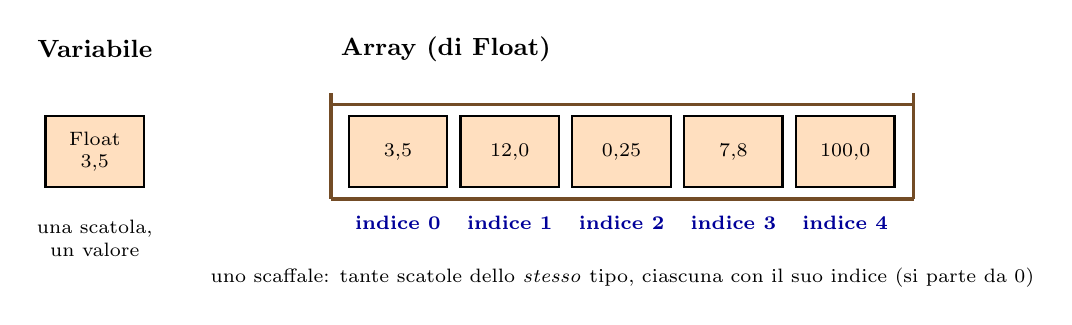
\begin{tikzpicture}[font=\footnotesize,
  ue7box/.style={draw, thick, fill=orange!25, minimum width=1.25cm, minimum height=0.9cm,
                 align=center, font=\scriptsize},
  ue7shelf/.style={draw, very thick, brown!60!black}]
  % variabile singola
  \node[font=\small\bfseries] at (0,2.3) {Variabile};
  \node[ue7box] (v) at (0,1.0) {Float\\3,5};
  \node[font=\scriptsize, align=center] at (0,-0.1) {una scatola,\\un valore};
  % array
  \begin{scope}[xshift=3.0cm]
    \node[font=\small\bfseries, anchor=west] at (0,2.3) {Array (di Float)};
    \draw[ue7shelf] (0,0.4) -- (7.4,0.4);
    \draw[ue7shelf] (0,1.6) -- (7.4,1.6);
    \draw[ue7shelf] (0,0.4) -- (0,1.75);
    \draw[ue7shelf] (7.4,0.4) -- (7.4,1.75);
    \node[ue7box] at (0.85,1.0) {3,5};
    \node[ue7box] at (2.27,1.0) {12,0};
    \node[ue7box] at (3.69,1.0) {0,25};
    \node[ue7box] at (5.11,1.0) {7,8};
    \node[ue7box] at (6.53,1.0) {100,0};
    \foreach \x/\i in {0.85/0, 2.27/1, 3.69/2, 5.11/3, 6.53/4} {
      \node[font=\scriptsize\bfseries, text=blue!60!black] at (\x,0.1) {indice \i};
    }
    \node[font=\scriptsize, align=center] at (3.7,-0.6) {uno scaffale: tante scatole
      dello \emph{stesso} tipo, ciascuna con il suo indice (si parte da 0)};
  \end{scope}
\end{tikzpicture}
\caption{La metafora del docente. Una variabile è una scatola che contiene un valore; un
array è uno scaffale che contiene tante scatole dello stesso tipo. Ogni posto dello
scaffale ha un indice, e il primo indice è 0. Schema ricostruito.}
\label{ue7:fig:scaffale}
\end{figure}

\paragraph{Approfondimento: array, set e map.} Romero e Sewell (capitolo 13, ``Data
Structures and Flow Control'') chiamano \textbf{contenitori} (\emph{containers}) le
strutture che raccolgono più valori dello stesso tipo, e nei Blueprint ce ne sono tre.
L'\textbf{array} è una lista ordinata con accesso per \textbf{indice}, ``e gli array
partono sempre dall'indice 0'': con quattro elementi, il primo ha indice 0 e l'ultimo
indice 3, cioè \emph{Length}~$-$~1. Il \textbf{set} è un insieme senza ordine e senza
doppioni, in cui si cerca per valore; la \textbf{map} associa a ogni \emph{chiave} un
\emph{valore} (per esempio il nome di un'arma e le sue munizioni). Sugli array si lavora
con una manciata di nodi: \textbf{Get (a copy)} legge l'elemento a un indice,
\textbf{Set Array Elem} lo modifica, \textbf{Add} aggiunge in fondo, \textbf{Insert}
inserisce a un indice spostando gli altri, \textbf{Length} e \textbf{Last Index} dicono
quanto è lungo, \textbf{Random Array Item} pesca un elemento a caso. Gli autori
avvertono: mai leggere un indice oltre l'ultimo, perché i risultati sono imprevedibili.
La tabella~\ref{ue7:tab:contenitori} riassume i quattro modi in cui una variabile può
essere costituita.

% ---------------------------------------------------------------------
\section{L'ereditarietà: parent e child}
\label{ue7:sec:ereditarieta}

La slide successiva riprende rapidamente le collisioni (``ripasseremo anche un po' le
collisioni'') e introduce il secondo concetto della giornata. ``Qualcuno di voi ha mai
sentito parlare dei concetti di \textbf{parent} e \textbf{child} in programmazione?''

\paragraph{Padre e figlio.} ``Mettiamo un esempio che possiamo vedere nella vita di tutti
i giorni'': il rapporto fra genitori e figli. ``Io, come figlio di mio padre, ho preso
una parte dei geni di mio padre'' (e di mia madre), ``e però, come essere unico, posso
variare nelle mie particolarità: non sono uguale, ma condivido comunque delle cose''.
Lo stesso succede con gli oggetti: ``ci sono degli oggetti che possono essere figli di
altri oggetti''. Esempio: un cubo \emph{parent} che nel Begin Play stampa un valore, e
fa solo quello. ``Il child mi stamperà sempre quel valore, ma magari stampa anche un
altro valore'': ``prende la caratteristica del papà, ma volendo può aggiungere, o
addirittura \textbf{sovrascrivere}, alcune azioni''.

\paragraph{Il cubo che diventa cilindro.} In Unreal i child si creano direttamente
dall'engine. In slide c'è il BP\_Cube delle lezioni precedenti: ``vogliamo farlo
diventare un cilindro? Creiamo un child e cambiamo semplicemente la Static Mesh''. ``Il
parent rimarrà un cubo, invece il figlio ha voluto cambiare forma'': per le
caratteristiche di Blueprint avranno lo stesso comportamento, ``oppure, volendo, lo
possiamo anche cambiare''. La figura~\ref{ue7:fig:gerarchia} mostra la gerarchia che si
costruirà oggi.

\begin{figure}[htbp]
\centering
\begin{tikzpicture}[font=\footnotesize,
  ue7cls/.style={draw, thick, rounded corners=4pt, align=center, fill=gray!8,
                 text width=3.3cm, minimum height=1.0cm, inner sep=4pt},
  ue7inh/.style={-{Triangle[open, length=3mm, width=3mm]}, thick}]
  \node[ue7cls, fill=gray!20] (actor) at (0,3.0) {\textbf{Actor}\\(classe di Unreal)};
  \node[ue7cls, fill=blue!10] (act) at (0,1.0) {\textbf{BP\_Activable}\\eventi
    Activation e Deactivation (Print String)};
  \node[ue7cls, fill=yellow!25] (light) at (-4.4,-1.4) {\textbf{BP\_ActivableLight}\\Point
    Light; override: accende e spegne};
  \node[ue7cls, fill=green!12] (ball) at (0,-1.4) {\textbf{BP\_BallMoving}\\(esercizio)
    override: Play e Reverse};
  \node[ue7cls, fill=orange!15] (plat) at (4.4,-1.4) {\textbf{piattaforma
    attivabile}\\(esercizio e compito)};
  \node[ue7cls, fill=gray!8] (btn) at (5.2,3.0) {\textbf{BP\_Button}\\array
    ActivableItems di tipo BP\_Activable};
  \draw[ue7inh] (act) -- (actor);
  \draw[ue7inh] (light.north) -- ++(0,0.6) -| (act.south);
  \draw[ue7inh] (ball) -- (act);
  \draw[ue7inh] (plat.north) -- ++(0,0.6) -| (act.south);
  \draw[ue7inh] (btn) -- (actor);
  \draw[-{Stealth[length=2.2mm]}, thick, dashed, violet!60!black] (btn.south) to[bend
    left=10] node[pos=0.45, right, font=\scriptsize, align=left]{contiene referenze\\a
    qualunque child} (act.east);
\end{tikzpicture}
\caption{La gerarchia di classi costruita nella lezione. Le frecce con la punta vuota
vanno dal child al parent (``eredita da''). BP\_Activable definisce i due eventi comuni;
ogni child li ridefinisce a modo suo. BP\_Button tiene un array di referenze di tipo
BP\_Activable, e quindi può contenere qualunque child. I nomi dei Blueprint
dell'esercizio sono quelli suggeriti dal docente; schema ricostruito.}
\label{ue7:fig:gerarchia}
\end{figure}

\paragraph{Approfondimento: superclasse, sottoclasse e tipo.} Romero e Sewell (capitolo
3, ``Object-Oriented Programming and the Gameplay Framework'') danno la versione
tecnica. Quando si crea un Blueprint, la prima cosa che si sceglie è la sua
\textbf{classe parent} (la \emph{superclasse}); un Blueprint ha \emph{un solo} parent,
ma può avere molti child (\emph{sottoclassi}). Il loro esempio sono le armi: una classe
base \emph{Weapon} con tutto ciò che è comune, e le armi concrete come figlie. Il
vantaggio è doppio. Da un lato, una funzione definita nel parent (\emph{Fire}) può
essere \textbf{ridefinita} (\emph{override}) in ogni child (il fucile a energia spara un
raggio, il lanciarazzi un razzo), e a runtime viene eseguita la versione della classe
effettiva dell'oggetto. Dall'altro, un child \textbf{è anche} del tipo del parent:
un'istanza del lanciarazzi è un \emph{Weapon}, e una variabile o un parametro di tipo
Weapon può contenerla. È esattamente il trucco su cui si regge il pulsante di oggi: una
variabile di tipo \emph{BP\_Activable} potrà contenere una luce, una piattaforma, una
palla, qualunque child degli attivabili. Del resto, ogni Blueprint della lezione è già un
child: BP\_Button ha come parent la classe \emph{Actor}.

% ---------------------------------------------------------------------
\section{La dimostrazione: il pulsante finito}
\label{ue7:sec:demo}

``Andremo a creare un bellissimo pulsantone. Eccolo qua.'' Nella scena del docente c'è
il risultato finale. Il giocatore sale sulla pedana, la pedana si abbassa e
\textbf{accende una luce} (``vedremo anche un pochino di \emph{lighting}''); se scende,
la luce si spegne. Nella stessa scena c'è una piattaforma che reagisce allo stesso
pulsante: ``ho creato una piattaforma di tipologia \textbf{attivabile}'', e luce e
piattaforma ``condividono'' qualcosa, ``sono della stessa classe, ma comportamenti
diversi''. Collegata la piattaforma al pulsante, la pressione accende la luce
\emph{e} manda giù la piattaforma; ``in questo caso ho fatto sì che andasse solo giù'':
quando la piattaforma è in basso ci si sale sopra, e lei torna su; si torna sul
pulsante, e di nuovo giù.

\paragraph{La domanda sull'interazione.} ``Faremo anche le interazioni, tipo premi E per
interagire?'' Sì: la prossima lezione sarà sulle \textbf{animazioni}, con un personaggio
animato, e l'interazione si farà con il \textbf{trace}, ``infatti il trace è collegato
al fatto dell'interazione'': ha interagito o non ha interagito.

\paragraph{Approfondimento: overlap o tasto?} I due modi di attivare qualcosa hanno usi
diversi. L'\emph{overlap} di un volume, quello di oggi, è passivo: scatta perché il
giocatore \emph{è} in un posto (pedane a pressione, trappole, cutscene). L'interazione
con un tasto è attiva: il giocatore guarda un oggetto e preme. Lo schema tipico, che la
lezione annuncia, è un \emph{line trace} dalla telecamera in avanti, eseguito alla
pressione del tasto; se colpisce un actor che ``sa'' interagire, gli si chiama un evento.
Per chiamarlo senza sapere in anticipo che classe abbia l'oggetto colpito si usa di
solito una \textbf{Blueprint Interface} (Romero e Sewell, capitolo 16): una lista di
funzioni senza corpo, che ogni classe interessata implementa a modo suo. È una cugina
dell'ereditarietà vista oggi, utile quando le classi da accomunare non hanno un parent
comune.

% ---------------------------------------------------------------------
\section{Il pulsante: due mesh e una box}
\label{ue7:sec:bottone}

``Allora, ragazzi, vi chiedo se siete pronti con il vostro progettino.'' Prima di
cominciare, la raccomandazione di sempre: tenere il progetto ordinato in
\textbf{cartelle}, ``perché se no un giorno succederà che non ritroverete'' le cose,
``come perdere qualcuno in un centro commerciale il sabato''. Nella cartella
\emph{Blueprint}, ``siamo al solito'': Blueprint Class, Actor. Il docente lo chiama
\textbf{BP\_Button1} (``io farò sempre il mio bellissimo BP\_Button1''); nel capitolo è
BP\_Button.

\paragraph{Due Static Mesh, non una.} ``Il bottone, per come sono fatte le mesh, sono due
Static Mesh'': una è il \textbf{frame}, la cornice, e l'altra la \textbf{piastra} che si
abbassa. Il docente le crea con Ctrl+C e Ctrl+V da un componente Static Mesh, e le
rinomina \textbf{Frame} e \textbf{Platform}; nel campo \emph{Static Mesh} assegna alla
prima la mesh della cornice della pedana a pressione (``se non sbaglio \emph{pressure
plate frame}'') e alla seconda quella della piastra (``\emph{pressure plate}\ldots{}
platform''); i nomi esatti degli asset nel progetto del corso non sono sicuri dalla
trascrizione. ``Essendo che sono fatti all'unisono'', i due pezzi sono già allineati.

\paragraph{Un consiglio per i 3D artist.} Il motivo della divisione vale per chiunque
modelli, o faccia modellare, oggetti interattivi. ``Se dovete fare un pulsante, non fate
fare un pulsante unico: fate fare un pulsante che è diviso'' fra la cornice (``quello che
sta attorno'') e la \emph{pressure plate}. ``Perché se adesso andiamo ad abbassare, ed è
un unico asset, tutto il bottone va giù, anche il frame, quindi si va a compenetrare col
pavimento.'' La regola: ``se ci sono delle cose interagibili a livello di movimentazione,
sappiate che è meglio sempre \textbf{splittarle}''. Poi, certo, ``dipende dalla
creatività'' e dal designer.

\paragraph{La box.} Terzo componente, ``la mitica'' \textbf{Box Collision}, scalata
perché sia ``leggermente unanime'' con il bottone, cioè della sua stessa impronta, e
alzata sull'asse Z: ``ricordatevi, attenzione a sotto''. E soprattutto, come per la
piattaforma della volta scorsa, \textbf{figlia della Platform}: ``la box deve seguire la
platform. Importante, in modo tale che se io sposto, si sposta con essa''
(figura~\ref{ue7:fig:bottone}).

\paragraph{È la box a comandare.} Una studentessa chiede conferma: ``bisogna fare la box
sopra perché è la box che interagisce, giusto?'' Sì: il player entra con i piedi nella
box, la box interagisce, la timeline parte e il pulsante va giù. ``Non è tanto la
piattaforma o il pulsante a triggerare l'evento, ma la box sopra.'' E perché non usare
l'overlap della mesh stessa? ``Perché le collisioni sono \textbf{troppo precise}'': sono
``a contatto con una superficie'', ``un controllo sempre più micro'', ``forse sì, forse
no'', e ``la possibilità di errore è molto più ampia''. Un volume, invece, dà una
risposta macro: ``sì, no''.

\begin{figure}[htbp]
\centering
\begin{tikzpicture}[font=\footnotesize,
  ue7comp/.style={draw, thick, rounded corners=3pt, align=left, fill=gray!8,
                  minimum height=0.6cm, text width=3.4cm, inner sep=4pt},
  ue7tree/.style={thick, gray!70!black}]
  \node[font=\small\bfseries, anchor=west] at (-0.2,1.0) {Components di BP\_Button};
  \node[ue7comp, anchor=west] (root) at (0,0.2) {DefaultSceneRoot};
  \node[ue7comp, anchor=west, fill=gray!20] (fr) at (0.6,-0.6) {\textbf{Frame}
    (Static Mesh)};
  \node[ue7comp, anchor=west, fill=blue!10] (pl) at (0.6,-1.4) {\textbf{Platform}
    (Static Mesh)};
  \node[ue7comp, anchor=west, fill=green!12] (bx) at (1.2,-2.2) {\textbf{Box} (Box
    Collision)};
  \node[ue7comp, anchor=west, fill=red!10] (tl) at (0,-3.0) {\textbf{PushButton}
    (Timeline)};
  \draw[ue7tree] (0.2,-0.1) |- (fr.west);
  \draw[ue7tree] (0.2,-0.1) |- (pl.west);
  \draw[ue7tree] (0.8,-1.7) |- (bx.west);
  % vista laterale
  \begin{scope}[xshift=7.4cm, yshift=-1.3cm]
    \draw[thick, gray] (-1.2,-1.0) -- (4.4,-1.0);
    \node[font=\scriptsize, gray] at (3.9,-1.25) {pavimento};
    \fill[gray!45, draw=black, thick] (-0.1,-1.0) rectangle (3.1,-0.75);
    \node[font=\scriptsize] at (1.5,-1.25) {Frame};
    \fill[blue!25, draw=blue!50!black, thick] (0.2,-0.75) rectangle (2.8,-0.5);
    \draw[thick, dashed, blue!50!black] (0.2,-0.85) rectangle (2.8,-0.6);
    \node[font=\scriptsize, anchor=west] at (3.2,-0.55) {Platform};
    \draw[-{Stealth[length=1.6mm]}, thick, red!60!black] (1.5,-0.45) -- (1.5,-0.72);
    \node[font=\scriptsize, red!60!black, anchor=west] at (1.6,-0.25) {$-10$ su Z};
    \draw[thick, dashed, green!50!black, fill=green!8, fill opacity=0.6]
      (0.3,-0.5) rectangle (2.7,0.15);
    \node[font=\scriptsize, green!40!black] at (1.0,-0.17) {Box};
    % omino
    \draw[thick] (-0.7,0.35) circle (0.13);
    \draw[thick] (-0.7,0.22) -- (-0.7,-0.35);
    \draw[thick] (-0.7,-0.35) -- (-0.85,-1.0);
    \draw[thick] (-0.7,-0.35) -- (-0.55,-1.0);
    \node[font=\scriptsize] at (-0.7,0.7) {player};
  \end{scope}
\end{tikzpicture}
\caption{I componenti del pulsante. A sinistra la gerarchia: Frame e Platform sono due
Static Mesh separate; la Box Collision è figlia della Platform, così la segue; la
timeline PushButton compare tra i componenti. A destra la vista laterale: la piastra
scende di 10 unità dentro la cornice (tratteggio), mentre la cornice resta ferma.
Schema ricostruito; le proporzioni non sono quelle dell'asset.}
\label{ue7:fig:bottone}
\end{figure}

% ---------------------------------------------------------------------
\section{Le collisioni della Static Mesh: simple e complex}
\label{ue7:sec:collisioni}

``Poi, se non sbaglio, su questo asset c'è un problema.'' È quello sollevato a inizio
lezione: il pulsante, come la piattaforma, potrebbe avere ``una collisione un po' tanto
alta'' per il personaggio.

\paragraph{Il Max Step Height.} Nel personaggio del giocatore c'è una variabile,
\textbf{Max Step Height}, ``che non ci permette di andare sopra queste tipologie di
asset'' se sono più alte di un certo valore. Il docente prova sulla sua scena: a lui va
``benissimo'', ``perché guardate cosa ho fatto io per ovviare a questo problema''. A
qualcuno degli studenti il personaggio si blocca con i piedi? Pare di no, ``bene''; ma
``per accortezza'', visto che al docente è capitato, si sistema la collisione della mesh.

\paragraph{Approfondimento: Max Step Height e Walkable Floor.} I due parametri stanno nel
\emph{Character Movement Component} del personaggio. Il \textbf{Max Step Height}
(predefinito 45 unità, cioè 45 centimetri) è l'altezza massima di uno ``scalino'' che il
personaggio può salire camminando, senza saltare; il \textbf{Walkable Floor Angle}
(predefinito 44,765 gradi) è la pendenza massima su cui può camminare. Se il bordo della
collisione di un oggetto supera lo scalino, la capsula del personaggio ci sbatte contro
come contro un muro. Si può alzare lo scalino del personaggio, ma cambia il modo in cui
si muove ovunque; di solito conviene sistemare la collisione dell'oggetto, come fa la
lezione.

\paragraph{L'editor della Static Mesh.} Si seleziona la mesh della piastra e si clicca
sulla ``finestrella blu'', l'icona dell'asset nel campo Static Mesh, per aprire
l'\textbf{editor della Static Mesh}: ``la schermata in cui Unreal fa vedere tutte le
particolarità delle collisioni dell'asset stesso'', ``dati molto più \emph{insight} del
modello''.

\paragraph{Una parentesi sui LOD.} Fra i dati ci sono i \textbf{LOD}, i \emph{level of
detail}: ``quella pratica di abbassare la risoluzione degli asset quando sono distanti,
in modo tale da avere ottimizzazione''. ``Sono tipo a 200 metri da me? Abbassa la
qualità, perché pesa.'' Il corso non li userà, ma è bene sapere che esistono.

\paragraph{Simple e complex.} Dal menù \textbf{Show} in alto si visualizzano le
collisioni dell'asset, e ``ci sono due tipologie di collisioni''.
\begin{itemize}
  \item Le \textbf{simple}, in \textbf{verde}: forme semplici, ``usate per avere
        interazioni di base''. Sono quelle che Unreal usa normalmente quando si mette un
        asset nella viewport, ``per tempi e cose di ottimizzazione''.
  \item Le \textbf{complex}, ``questi lineamenti blu'' (azzurri): la forma esatta del
        modello, triangolo per triangolo. Servono quando ``ci serve l'esatto punto''
        in cui si tocca l'oggetto. Esempio: un \textbf{sistema di scalata}, in cui
        ``devo andare a vedere il punto esatto in cui ho messo la mano'' per tirare su il
        personaggio (``poi ci sono anche alternative'').
\end{itemize}
Le due collisioni si preparano ``durante la modellazione'', e chi segue il corso di 3D
art le vedrà. Ma attenzione: ``se mettete le complex collision su tutti gli asset,
probabilmente potete dire ciao al vostro bellissimo PC'', a meno di ottimizzazioni
parallele. Qui servono le simple.

\paragraph{Modificare la collisione.} La cosa bella è che le collisioni simple si
possono modificare a mano. Cliccando sul ``reticoletto verde'' si possono muovere,
ruotare e scalare come un oggetto qualsiasi. Gli studenti dovrebbero avere una
collisione ``un po' più arzigogolata'', ``con tutti i reticolini''; il docente ha già
modificato la sua. La procedura:
\begin{enumerate}
  \item \textbf{cancellare} la collisione simple esistente, ``quella verde, non quella
        azzurra'';
  \item dal menù \textbf{Collision} aggiungerne una nuova, scegliendo fra
        \textbf{Sphere}, \textbf{Capsule}, \textbf{Box} e le varie \textbf{k-DOP} (10DOP-X,
        Y, Z, 18DOP, 26DOP; nella trascrizione ``10 di OP meno X'');
  \item per il pulsante, \textbf{Box} (``Box Simplified Collision''): ``a noi ci serve
        una scatoletta, è un quadrato alla fine'';
  \item selezionare la box e \textbf{stringerla} ``proprio un'anticchia'', abbassandola,
        dopo aver tolto lo \emph{snap}, ``quasi come se fosse una collisione già
        abbassata''.
\end{enumerate}
Ora il pulsante ``ha una collisione un po' più affondabile''.

\paragraph{Le forme a confronto.} Il docente prova le alternative una per una. La
\textbf{sfera} su una piastra quadrata ``non ci serve assolutamente, perché non è
coerente alla sua forma''. Le \textbf{k-DOP} invece seguono il modello con un numero
crescente di piani: ``sono il livello di dettaglio che la collisione avrà, il livello di
vertici''; ``più vertici ci sono, più le collisioni sono precise, meno spigolose''. Sul
cubetto la 10DOP sulla X, sulla Y e sulla Z danno risultati quasi uguali, con ``piccole
differenze'' di taglio; la 18DOP ``ha fatto gli angoli più precisi''; la 26DOP, ``il
massimo'', taglia anche gli spigoli (figura~\ref{ue7:fig:kdop}).

\paragraph{Un'esperienza di lavoro.} ``A me è capitato con un lavoro che ho fatto.'' Nel
livello c'era una piccola pista, e alcuni asset avevano collisioni ``estremamente
complesse'': il docente e il gruppo di designer hanno dovuto \textbf{cancellare tutte le
collisioni e rifarle} a mano, ``con i cubettini'', per semplificare il lavoro
dell'engine. La morale: le collisioni sono parte del lavoro del level designer, non solo
del modellatore.

\begin{figure}[htbp]
\centering
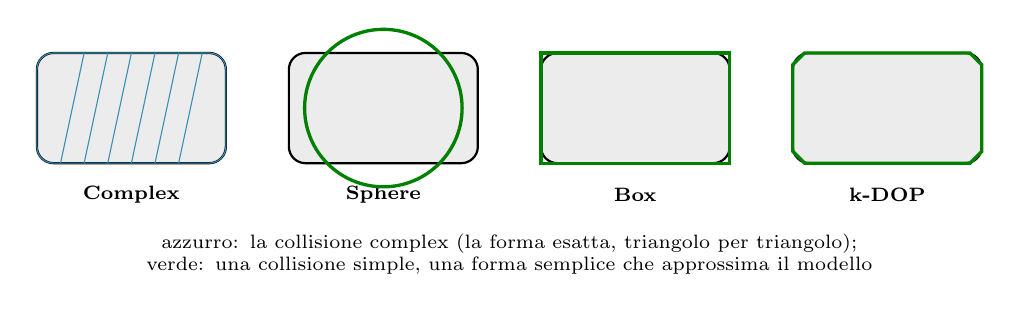
\begin{tikzpicture}[font=\footnotesize,
  ue7mesh/.style={draw=black, thick, fill=gray!15},
  ue7coll/.style={draw=green!50!black, very thick},
  ue7cplx/.style={draw=cyan!70!black, thin}]
  % modello: piastra con bordi smussati (vista dall'alto, stilizzata)
  \foreach \x/\nome in {0/Complex, 3.2/Sphere, 6.4/Box, 9.6/k-DOP} {
    \begin{scope}[xshift=\x cm]
      \draw[ue7mesh, rounded corners=6pt] (0,0) rectangle (2.4,1.4);
      \node[font=\scriptsize\bfseries] at (1.2,-0.4) {\nome};
    \end{scope}
  }
  % complex: segue tutto
  \draw[ue7cplx, rounded corners=6pt] (0,0) rectangle (2.4,1.4);
  \foreach \i in {0.3,0.6,...,2.1} {\draw[ue7cplx] (\i,0) -- (\i+0.3,1.4);}
  % sphere
  \draw[ue7coll] (4.4,0.7) circle (1.0);
  % box
  \draw[ue7coll] (6.4,0) rectangle (8.8,1.4);
  % kdop: ottagono
  \draw[ue7coll] (9.75,0) -- (11.85,0) -- (12.0,0.15) -- (12.0,1.25) -- (11.85,1.4)
    -- (9.75,1.4) -- (9.6,1.25) -- (9.6,0.15) -- cycle;
  \node[font=\scriptsize, align=center, text width=12cm] at (6.0,-1.15) {azzurro: la
    collisione complex (la forma esatta, triangolo per triangolo); verde: una collisione
    simple, una forma semplice che approssima il modello};
\end{tikzpicture}
\caption{Collisioni della piastra viste dall'alto, in forma stilizzata. La complex
segue ogni triangolo del modello; la Sphere non è coerente con la forma; la Box è la
scelta della lezione; le k-DOP aggiungono piani e smussano gli spigoli. Schema
ricostruito, non una schermata dell'editor.}
\label{ue7:fig:kdop}
\end{figure}

\paragraph{Approfondimento: Collision Complexity.} Nell'editor della Static Mesh, fra
i dettagli dell'asset, c'è l'impostazione \textbf{Collision Complexity}. Con il
valore predefinito (\emph{Project Default}, in pratica ``simple e complex separate'') le
query fisiche e il movimento dei personaggi usano la collisione simple, mentre i trace
che lo chiedono esplicitamente (il flag \emph{Trace Complex}) usano quella complex. Con
\emph{Use Complex Collision As Simple} la forma esatta viene usata per tutto: comodo per
un pavimento irregolare statico, ma costoso, e incompatibile con la simulazione fisica
dell'oggetto. Le k-DOP (\emph{discrete oriented polytope}) sono poliedri convessi che
racchiudono la mesh con 10, 18 o 26 piani a orientamento fisso; il menù
\emph{Collision} offre anche \emph{Auto Convex Collision}, che scompone la mesh in più
pezzi convessi, una via di mezzo fra la precisione della complex e il costo della
simple.

% ---------------------------------------------------------------------
\section{La timeline del pulsante}
\label{ue7:sec:timeline}

``Fatto questo, ritorniamo sul nostro bellissimo button e andiamo effettivamente a creare
quello che sarà il funzionamento di base'': il tasto si deve abbassare sulla Z.

\paragraph{Gli eventi e il controllo sul player.} ``Quello che abbiamo visto l'altra
volta'': con la Box selezionata, nella sezione degli eventi in fondo ai dettagli, si
creano \textbf{On Component Begin Overlap} e \textbf{On Component End Overlap}, ``tutti e
due''. Poi ``la solita cosa'': si verifica che sia il player, ``con Is Valid o con il
tag, ma noi facciamo più semplice''. Dall'\textbf{Other Actor} si tira fuori un
\textbf{==} (``uguale uguale'') con \textbf{Get Player Pawn}, e il risultato va in un
\textbf{Branch}.

\paragraph{La timeline.} Dal ramo True, ``abbiamo già detto che è una timeline quella
che useremo'': una nuova timeline, rinominata \textbf{PushButton}, avviata con
\textbf{Play from Start} (la differenza con Play si chiarirà nella
sezione~\ref{ue7:sec:play}). Quanto deve scendere il pulsante? Il docente lo misura
nella viewport: seleziona la piastra, attiva lo \emph{snap} (``molto meglio''), con passo
10, e la abbassa finché è ``totalmente abbassata''. Bastano \textbf{10 unità}: ``quindi
abbiamo capito che dovremmo abbassarla di 10''.

\paragraph{La curva.} Doppio clic sulla timeline. ``Il valore da mettere per la
lunghezza della timeline è \textbf{0,25 secondi}. È molto corto.'' Poi:
\begin{enumerate}
  \item una \textbf{float track};
  \item un punto (Shift e clic) a \textbf{tempo 0, valore 0};
  \item un secondo punto a \textbf{tempo 0,25} (``il massimo della nostra timeline'') e
        \textbf{valore $-$10}: ``farà un passaggio in 0,25 secondi da 0 a $-$10'';
  \item i due pulsantini \textbf{Zoom to Fit Horizontal} e \textbf{Zoom to Fit
        Vertical} (``le due freccine''), che adattano il grafico alla lunghezza e
        all'altezza della curva.
\end{enumerate}
Una domanda dalla chat (``come si chiama il pallino sulla timeline?'') riceve la risposta
già nota: Shift e clic. Rispetto alla piattaforma della volta scorsa c'è una differenza
importante: allora la traccia andava da 0 a 1 ed era un \emph{alfa} da dare a un Lerp;
oggi la traccia contiene \emph{direttamente} lo spostamento, in unità del mondo.

\paragraph{Il nome della traccia.} ``Abbiamo la New Track 0'': la si rinomina cliccandoci
sopra con \textbf{F2}, \textbf{PushButtonZ} (``facciamo una Z maiuscola''). Il pin sul
nodo prende lo stesso nome; a una studentessa resta scritto \emph{New Track 0} anche
dopo la rinomina, e il docente la rassicura: ``è solo il nome che gli abbiamo dato'', il
funzionamento non cambia.

\paragraph{Il movimento.} Nell'Event Graph:
\begin{itemize}
  \item dal pin \textbf{PushButtonZ} si crea un \textbf{Make Vector}, collegando il
        valore alla \textbf{Z} (``l'asse che ci interessa''); X e Y restano a 0, ``tanto
        la X è zero e rimane zero'';
  \item si trascina la Platform nel grafo e se ne tira fuori \textbf{Set Relative
        Location}, con il vettore in \emph{New Location}. ``È relative perché è
        relativa alla sua transform'': lo zero è quello della piastra dentro il
        Blueprint, non lo zero del mondo;
  \item il nodo va collegato all'\textbf{Update} della timeline.
\end{itemize}
In Play, sulla pedana, ``non esplode, vedete che si abbassa''. Ma non si rialza più:
``è normale''. Manca il ritorno: dall'\textbf{End Overlap}, con lo stesso controllo sul
player, si collega l'ingresso \textbf{Reverse} della timeline. ``Premuto, torna su;
premuto, torna su.'' ``Eccolo che abbiamo creato il nostro movimento del pulsante, non
ancora la sua funzionalità'' (figura~\ref{ue7:fig:grafobottone}).

\begin{figure}[htbp]
\centering
\begin{tikzpicture}[font=\footnotesize,
  ue7node/.style={draw, thick, rounded corners=4pt, align=center, fill=gray!8,
                  minimum height=0.8cm, text width=2.0cm},
  ue7ev/.style={ue7node, fill=red!12},
  ue7exec/.style={-{Stealth[length=2.5mm]}, very thick, black!80},
  ue7data/.style={-{Stealth[length=2mm]}, thick, violet!60!black}]
  \node[ue7ev, text width=2.6cm] (bo) at (0,1.2) {\textbf{On Component Begin
    Overlap} (Box)};
  \node[ue7ev, text width=2.6cm] (eo) at (0,-1.2) {\textbf{On Component End
    Overlap} (Box)};
  \node[ue7node, text width=1.9cm] (eq1) at (3.3,2.6) {Other Actor \textbf{==} Get
    Player Pawn};
  \node[ue7node, text width=1.3cm] (br1) at (3.3,1.2) {\textbf{Branch}};
  \node[ue7node, text width=1.3cm] (br2) at (3.3,-1.2) {\textbf{Branch}};
  \node[ue7node, text width=1.9cm] (eq2) at (3.3,-2.6) {Other Actor \textbf{==} Get
    Player Pawn};
  \node[ue7node, fill=red!8, text width=2.4cm, minimum height=2.6cm] (tl) at (7.3,0)
    {\textbf{Timeline}\\PushButton\\[2pt]\scriptsize 0,25 s\\da 0 a $-$10};
  \node[ue7node, text width=1.6cm] (mv) at (10.6,-1.4) {\textbf{Make Vector}\\X 0, Y 0};
  \node[ue7node, text width=2.3cm] (set) at (13.1,0.8) {Platform $\rightarrow$
    \textbf{Set Relative Location}};
  \draw[ue7exec] (bo) -- (br1);
  \draw[ue7exec] (eo) -- (br2);
  \draw[ue7data] (eq1) -- (br1);
  \draw[ue7data] (eq2) -- (br2);
  \draw[ue7exec] (br1.east) -- node[above, font=\scriptsize]{True} ++(0.7,0) |-
    node[pos=0.78, above, font=\scriptsize]{Play from Start} ([yshift=0.8cm]tl.west);
  \draw[ue7exec] (br2.east) -- node[below, font=\scriptsize]{True} ++(0.7,0) |-
    node[pos=0.78, below, font=\scriptsize]{Reverse} ([yshift=-0.8cm]tl.west);
  \draw[ue7exec] ([yshift=0.8cm]tl.east) -- node[above, font=\scriptsize]{Update}
    (set.west);
  \draw[ue7data] ([yshift=-0.6cm]tl.east) -- node[above, font=\scriptsize, pos=0.5]{PushButtonZ}
    ++(0.6,0) |- (mv.west);
  \draw[ue7data] (mv.east) -| node[pos=0.3, below, font=\scriptsize]{Z $\rightarrow$
    New Location} (set.south);
\end{tikzpicture}
\caption{Il movimento del pulsante. Il Begin Overlap della Box, se l'actor è il player,
fa partire la timeline PushButton da capo; l'End Overlap la manda in Reverse. A ogni
Update il valore della traccia (da 0 a $-$10 in 0,25 secondi) diventa la Z di un
vettore, e la piastra si sposta con Set Relative Location. Schema ricostruito.}
\label{ue7:fig:grafobottone}
\end{figure}

\paragraph{Approfondimento: perché qui niente Lerp.} La sesta lezione aveva mostrato il
metodo ``giusto'' per la piattaforma: una traccia da 0 a 1 usata come alfa di un Lerp
fra due posizioni salvate. Qui il docente sceglie la strada diretta, e funziona per due
ragioni. La prima: il valore della traccia è \emph{assoluto}, non si somma alla posizione
corrente, quindi non si accumula (era il difetto del primo metodo della volta scorsa).
La seconda: la piastra è figlia di una radice ferma, e la sua posizione relativa di
partenza è (0, 0, 0), quindi ``$-$10 rispetto alla radice'' vuol dire esattamente ``10
più in basso di dove sta''. Se la piastra fosse stata spostata nel Blueprint, per
esempio a Z 5, il primo Update la teletrasporterebbe a Z 0: in quel caso serve sommare
lo spostamento alla posizione iniziale salvata, o tornare al Lerp. Per oggetti che si
spostano di poco, una traccia in unità del mondo è la soluzione più leggibile.

% ---------------------------------------------------------------------
\section{Le curve: linear e auto}
\label{ue7:sec:curve}

``Adesso vi faccio vedere anche una particolarità, che potremmo usare anche per la
piattaforma'': si può \textbf{modificare la tipologia dei punti}.

\paragraph{Lineari.} I punti creati finora sono \textbf{lineari}: ``formano una linea'',
e l'aumento o la diminuzione del valore ``è sempre costante'' nel tempo: in ogni
frazione di secondo il valore cambia sempre della stessa quantità, ``tra un punto e
l'altro''.

\paragraph{Curve.} ``Se invece vogliamo una curva un po' più \emph{smooth}'', si fa tasto
destro su un punto: compare la serie di \textbf{Key Interpolation}, ``cioè ti dice: quale
tipo di punto vuoi che sia?''. Il docente sceglie \textbf{Auto}, e la linea diventa una
curva; lo stesso sull'altro punto. Ora, con i ``piccoli braccetti'' (le tangenti) di
ciascun punto, si può modellare ``come nel tempo questa linea va da punto A a punto B''
(figura~\ref{ue7:fig:curve}, tabella~\ref{ue7:tab:interp}).

\paragraph{A che cosa serve.} Una studentessa chiede che cosa cambi in pratica. Il
docente prova: allunga la timeline a 1 secondo e piega la curva in modo che superi il
valore finale e poi ci ritorni. Il risultato, con un'escursione di appena 10 unità, sono
``micro movimenti'': il pulsante ``fa boom e ritorna su'', ``su e giù e si abbassa''.
``Cambiare la forma della curva ci permette di creare dei piccoli intervalli di vario
tipo'': il movimento rallenta, accelera, rimbalza. Su un pulsante si vede poco (``è molto
piccolo come spazio''); ``magari in pausa'' il docente propone di mostrarlo con ``una
piccola sferetta che fa su e giù''. Poi rimette la curva com'era.

\begin{figure}[htbp]
\centering
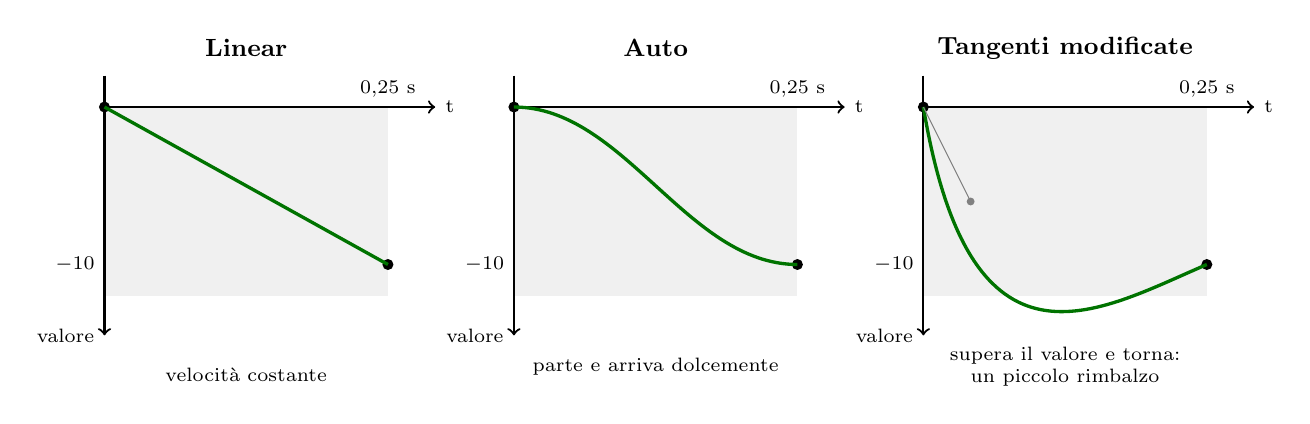
\begin{tikzpicture}[font=\footnotesize]
  \foreach \x/\titolo in {0/Linear, 5.2/Auto, 10.4/Tangenti modificate} {
    \begin{scope}[xshift=\x cm]
      \fill[gray!12] (0,-2.4) rectangle (3.6,0);
      \draw[->, thick] (0,0) -- (4.2,0) node[right, font=\scriptsize]{t};
      \draw[->, thick] (0,0.4) -- (0,-2.9) node[left, font=\scriptsize]{valore};
      \node[font=\scriptsize, left] at (0,-2.0) {$-10$};
      \node[font=\scriptsize, above] at (3.6,0) {0,25 s};
      \node[font=\small\bfseries] at (1.8,0.75) {\titolo};
      \fill (0,0) circle (0.07);
      \fill (3.6,-2.0) circle (0.07);
    \end{scope}
  }
  \draw[very thick, green!45!black] (0,0) -- (3.6,-2.0);
  \draw[very thick, green!45!black] (5.2,0) .. controls (6.6,0) and (7.4,-2.0) ..
    (8.8,-2.0);
  \draw[very thick, green!45!black] (10.4,0) .. controls (11.0,-3.6) and (12.6,-2.6) ..
    (14.0,-2.0);
  \draw[gray, thin] (10.4,0) -- (11.0,-1.2);
  \fill[gray] (11.0,-1.2) circle (0.05);
  \node[font=\scriptsize, align=center] at (1.8,-3.4) {velocità costante};
  \node[font=\scriptsize, align=center] at (7.0,-3.3) {parte e arriva dolcemente};
  \node[font=\scriptsize, align=center] at (12.2,-3.3) {supera il valore e torna:\\un
    piccolo rimbalzo};
\end{tikzpicture}
\caption{La stessa traccia con tre interpolazioni. Con le key lineari il pulsante scende
a velocità costante; con Auto la curva è morbida agli estremi; trascinando le tangenti
(i ``braccetti'') si ottengono andamenti come il rimbalzo provato a lezione. Schema
ricostruito.}
\label{ue7:fig:curve}
\end{figure}

\begin{table}[htbp]
\centering
\small
\begin{tabular}{@{}p{3.0cm}p{11.0cm}@{}}
\toprule
\textbf{Key Interpolation} & \textbf{Andamento fino alla key successiva} \\
\midrule
Auto & curva morbida, con tangenti calcolate in automatico (la scelta della lezione) \\
User & curva morbida con tangenti impostate a mano trascinando i ``braccetti'' \\
Break & come User, ma le due tangenti del punto si muovono in modo indipendente
(spigoli voluti) \\
Linear & retta: variazione costante nel tempo (il comportamento predefinito dei punti
creati con Shift e clic) \\
Constant & il valore resta fermo e salta alla key successiva al suo arrivo (a
gradino) \\
\bottomrule
\end{tabular}
\caption{I tipi di interpolazione di una key, dal menù del tasto destro su un punto della
timeline. La lezione usa Linear e Auto; le altre voci sono un'integrazione basata
sull'editor di Unreal Engine 5.}
\label{ue7:tab:interp}
\end{table}

\paragraph{Approfondimento: \emph{easing} e \emph{game feel}.} Le curve sono lo strumento
più economico per dare \emph{peso} a un movimento. In animazione si parla di
\emph{ease in} e \emph{ease out} (partire e arrivare lentamente) e di
\emph{overshoot} (superare la meta e tornare indietro, come il rimbalzo provato dal
docente): una porta che rallenta prima di chiudersi, un pulsante che affonda di colpo e
risale con un piccolo rimbalzo, un ascensore che parte dolcemente. A parità di durata,
un movimento lineare appare meccanico, uno con l'\emph{easing} appare fisico. Nelle
timeline la curva è anche un \emph{asset} riutilizzabile: dall'editor la traccia si può
salvare come \textbf{Curve Float} esterna e usare in più timeline, così tutti i pulsanti
del gioco si muovono allo stesso modo e si correggono in un punto solo.

% ---------------------------------------------------------------------
\section{I problemi degli studenti con il pulsante}
\label{ue7:sec:problemibottone}

``Il mio bottone non scende.'' ``Neanche a me.'' Il docente ripassa il grafo (Platform,
Set Relative Location sull'Update, il pin della traccia nella Z del Make Vector) e poi
chiama le studentesse in condivisione, una alla volta, ``Lucrezia per prima''. La
condivisione dello schermo su Zoom richiede diversi tentativi, fra permessi da dare,
barre degli strumenti che spariscono e un'eco ``quasi un boomerang''; alla fine
funziona.
\begin{itemize}
  \item \textbf{Il volume.} La box è ``molto piccola'' e il volume ``troppo basso'': deve
        stare sopra la piastra.
  \item \textbf{I punti della curva.} Il primo punto non sta a tempo 0: ``devi mettere
        tempo zero, valore zero''; il secondo a 0,25 e $-$10 ``va benissimo''. E le due
        freccine dello Zoom to Fit aiutano a vedere davvero la curva.
  \item \textbf{La lunghezza.} Un'altra studentessa ha messo 0,25 nel tempo del punto ma
        ha lasciato la \textbf{Length} della timeline al valore predefinito: ``devi
        modificare la lunghezza; vedi, c'è scritto \emph{Length} sopra''.
  \item \textbf{Stop invece di Reverse.} Sull'End Overlap era collegato \emph{Stop}: il
        pulsante si ferma dov'è invece di tornare su.
  \item \textbf{L'Update scollegato.} Il caso più istruttivo: il Set Relative Location
        aveva il pin dei dati collegato, ma non quello di \textbf{esecuzione}
        all'Update. ``Qui devi collegare solo l'execution pin.'' ``Ricordati, fai conto
        che l'Update è quello che fa'' il lavoro nel tempo della linea del tempo.
\end{itemize}
Un consiglio di contorno: ``spostati un po' gli asset'' di prova delle lezioni
precedenti, che potrebbero dare fastidio ai ``grubetti'' (forse i cubetti della
matrice).

\paragraph{Approfondimento: dati senza esecuzione.} L'ultimo errore è il più tipico di chi
viene da altri strumenti. Nei Blueprint i \textbf{pin di dati} (colorati) dicono
\emph{con che cosa} lavora un nodo, i \textbf{pin di esecuzione} (bianchi) dicono
\emph{quando} il nodo viene eseguito. Un nodo con i soli dati collegati non viene mai
eseguito: i suoi ingressi verrebbero calcolati se qualcuno lo chiamasse, ma nessuno lo
chiama. Fanno eccezione i nodi \emph{pure}, senza pin bianchi (come Make Vector o
Get Player Pawn), che vengono calcolati quando un nodo eseguito ne legge l'uscita. Il
controllo da fare quando ``non succede niente'' è quindi sempre lo stesso: seguire il
filo bianco dall'evento fino all'ultimo nodo.

% ---------------------------------------------------------------------
\section{Play o Play from Start?}
\label{ue7:sec:play}

``Posso fare una domanda rapidissima? Perché abbiamo usato Play from Start e non
Play?'' La risposta del docente, con un esempio di timeline da 0 a 2 secondi.
\begin{itemize}
  \item Con \textbf{Play}, se ci si ferma a 1 secondo (si esce dal pulsante quando la
        piastra ``sta a metà'') e poi si rientra, la timeline ``continuerà da quel punto
        in particolare dove ci siamo fermati'': da 1 a 2.
  \item Con \textbf{Play from Start}, se si esce e si rientra, la timeline ``riparte da
        0, non da 1''.
\end{itemize}
Nel caso del pulsante, dice il docente, ``non abbiamo particolari interruzioni, perché
abbiamo proprio un \emph{in} e \emph{out}''.

\paragraph{Approfondimento: che cosa succede davvero con il Reverse.} Con un pulsante
così breve la differenza si nota poco, ma esiste, ed è utile capirla con la
figura~\ref{ue7:fig:play}. Si entra, la timeline va avanti; si esce a metà, e il Reverse
la fa tornare indietro \emph{da dove si trova}. Se si rientra prima che sia tornata a 0:
\begin{itemize}
  \item con \textbf{Play} la timeline inverte di nuovo la direzione dal punto in cui è,
        e la piastra riprende a scendere senza scatti;
  \item con \textbf{Play from Start} la timeline salta a 0: la piastra torna di colpo in
        alto e riparte a scendere, un piccolo scatto visibile.
\end{itemize}
Per oggetti che vanno avanti e indietro seguendo un ingresso e un'uscita (pulsanti,
porte, piattaforme) la coppia più naturale è quindi \textbf{Play} e \textbf{Reverse}; è
proprio quella che il docente raccomanderà nell'esercizio finale
(sezione~\ref{ue7:sec:esercizio}) e che correggerà nella soluzione di uno studente
(``mettilo su Play, non Play from Start''). Play from Start serve quando ogni attivazione
deve ripetere l'animazione da capo, per esempio un colpo o un lampo.

\begin{figure}[htbp]
\centering
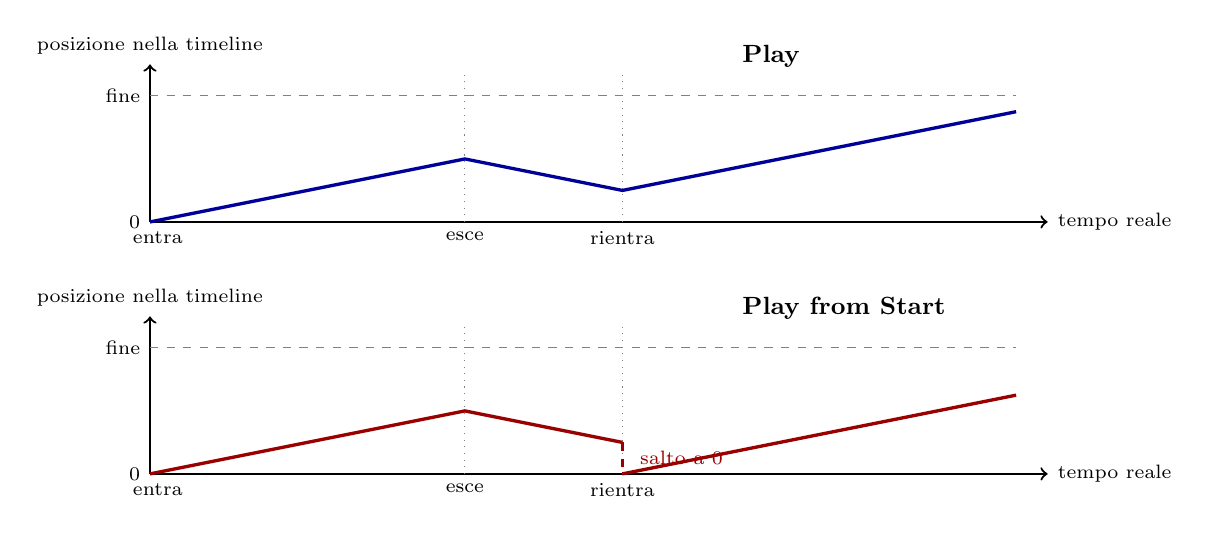
\begin{tikzpicture}[font=\footnotesize, x=1.0cm, y=1.0cm]
  \foreach \y/\titolo in {0/Play, -3.2/Play from Start} {
    \begin{scope}[yshift=\y cm]
      \draw[->, thick] (0,0) -- (11.4,0) node[right, font=\scriptsize]{tempo reale};
      \draw[->, thick] (0,0) -- (0,2.0) node[above, font=\scriptsize]{posizione nella
        timeline};
      \draw[gray, dashed] (0,1.6) -- (11,1.6);
      \node[font=\scriptsize, left] at (0,1.6) {fine};
      \node[font=\scriptsize, left] at (0,0) {0};
      \node[font=\small\bfseries, anchor=west] at (7.4,2.1) {\titolo};
      \draw[gray, dotted] (4,0) -- (4,1.9);
      \draw[gray, dotted] (6,0) -- (6,1.9);
      \node[font=\scriptsize, below] at (0.1,0) {entra};
      \node[font=\scriptsize, below] at (4,0) {esce};
      \node[font=\scriptsize, below] at (6,0) {rientra};
    \end{scope}
  }
  % Play
  \draw[very thick, blue!60!black] (0,0) -- (4,0.8) -- (6,0.4) -- (11,1.4);
  % Play from start
  \draw[very thick, red!60!black] (0,-3.2) -- (4,-2.4) -- (6,-2.8);
  \draw[very thick, red!60!black, dashed] (6,-2.8) -- (6,-3.2);
  \draw[very thick, red!60!black] (6,-3.2) -- (11,-2.2);
  \node[font=\scriptsize, red!60!black, anchor=west] at (6.1,-3.0) {salto a 0};
\end{tikzpicture}
\caption{Entrare, uscire a metà e rientrare prima che la timeline sia tornata a 0. Con
Play (in alto) la timeline riprende da dove si trova; con Play from Start (in basso)
salta all'inizio, e l'oggetto fa uno scatto. Schema ricostruito come integrazione alla
risposta del docente.}
\label{ue7:fig:play}
\end{figure}

% ---------------------------------------------------------------------
\section{Gli attivabili: la classe BP\_Activable}
\label{ue7:sec:activable}

``Adesso andiamo a fare una cosa bellina.'' Il pulsante si muove, ma non fa ancora
niente. Prima di creare la luce, ``prima, importante'', serve una \textbf{tipologia di
actor}: quella degli \textbf{attivabili}, ``quelli che per noi saranno gli attivabili''.

\paragraph{La classe base.} Un nuovo Blueprint Class di tipo Actor: il docente lo chiama
BP\_Activable1, qui è semplicemente \textbf{BP\_Activable}. ``Che succede qui all'interno? Ci serve solo
questo'': con la sola creazione ``abbiamo intanto definito una tipologia di actor''.
Dentro, due \textbf{Custom Event}:
\begin{itemize}
  \item \textbf{Activation}, collegato a un Print String ``attivato'';
  \item \textbf{Deactivation}, collegato a un Print String ``deattivato'' (cioè
        disattivato).
\end{itemize}
``Questi due eventi saranno collegati all'attivare qualcosa o disattivare qualcosa.'' Le
due stampe sono provvisorie: servono a vedere che il collegamento funziona, e poi a
capire come i figli possono \emph{sovrascrivere} gli eventi del padre
(sezione~\ref{ue7:sec:override}).

\paragraph{La domanda.} ``Quando è che io lo devo chiamare? E soprattutto, come faccio a
fargli dire: ehi, bottone, guarda che devi attivare questo esatto elemento?'' La risposta
è una variabile nel bottone, ed è il cuore della lezione.

% ---------------------------------------------------------------------
\section{Il bottone e la lista degli attivabili}
\label{ue7:sec:array}

\paragraph{Una variabile di tipo BP\_Activable.} Nel Blueprint del bottone si crea una
variabile, \textbf{ActivableItems}, e se ne cambia il tipo. ``Questo è molto
interessante, ragazzi: possiamo creare una variabile del tipo di quell'asset che abbiamo
appena creato'': il tipo è \textbf{BP\_Activable}, nella forma \emph{Object Reference}.
Una variabile così non contiene un numero o un testo, ma un \textbf{riferimento} a un
attivabile presente nel livello.

\paragraph{Pubblica.} ``Facciamola \textbf{pubblica}, e si fa con questo
\textbf{occhietto}'' accanto alla variabile. Il docente mette nel livello un
BP\_Activable e seleziona il pulsante: nei Details, in \emph{Default}, ``è apparso
Activable Items''. ``Vuol dire che questa variabile è modificabile dai Details del nostro
editor'', e quindi ``ci permette di avere interazioni dirette con la viewport,
l'ambiente di gioco'': ogni copia del pulsante nel livello può avere i suoi oggetti da
attivare.

\paragraph{Un array.} ``All'inizio di lezione abbiamo parlato degli array'': il pulsante
non deve attivare un oggetto solo, ``ma una moltitudine di oggetti''. Si cambia quindi
non la \emph{tipologia} della variabile, ma la sua \textbf{costituzione} (``cerchiamo di
dividerli'', precisa il docente): accanto al \emph{Variable Type} c'è un'icona (``questo
cilindro, vabbè, un'ellisse'') con una freccetta, e il menù offre \textbf{Single},
\textbf{Array}, \textbf{Set} e \textbf{Map} (tabella~\ref{ue7:tab:contenitori}). Si sceglie
Array, e l'icona della variabile cambia: ``diventa una matrice'', una griglia di
quadratini. ``Adesso abbiamo una variabile array di tipologia BP\_Activable.''

\begin{table}[htbp]
\centering
\small
\begin{tabular}{@{}p{2.4cm}p{5.8cm}p{5.8cm}@{}}
\toprule
\textbf{Costituzione} & \textbf{Che cosa contiene} & \textbf{Esempio} \\
\midrule
Single & un valore solo (la ``scatola'') & la referenza a una sola luce \\
Array & una lista ordinata di valori dello stesso tipo, con indice da 0; ammette
doppioni & gli oggetti attivati dal pulsante (ActivableItems) \\
Set & un insieme di valori unici, senza ordine e senza indice & i nomi degli oggetti
già raccolti \\
Map & coppie chiave--valore, con chiavi uniche & il nome di un'arma e le sue
munizioni \\
\bottomrule
\end{tabular}
\caption{Le quattro costituzioni di una variabile, dal menù accanto al Variable Type.
La lezione usa Single e Array; le descrizioni di Set e Map seguono Romero e Sewell
(capitolo 13).}
\label{ue7:tab:contenitori}
\end{table}

\paragraph{Quando chiamare gli attivabili.} ``Vogliamo che quando il nostro bel bottone
finisce di fare il suo percorso, e si schiaccia'', partano le attivazioni: si usa
l'uscita \textbf{Finished} della timeline. Ma Finished scatta sia alla fine della
discesa sia alla fine della risalita (dopo il Reverse), quindi bisogna sapere ``che
direzione è''. ``Vi ricordate che abbiamo usato lo Switch l'altra volta sulla
Direction?'' Dal pin \textbf{Direction} si crea uno \textbf{Switch on
ETimelineDirection}, collegato al Finished:
\begin{itemize}
  \item \textbf{Forward}: la timeline è andata avanti, il pulsante è schiacciato,
        quindi \textbf{attiva};
  \item \textbf{Backward}: la timeline è tornata indietro, il pulsante è tornato
        ``alla sua posizione di prima'', quindi \textbf{disattiva}.
\end{itemize}

\paragraph{Il For Each Loop.} ``Abbiamo già visto il For Loop. Questo è il \textbf{For
Each Loop}.'' Si prende un \emph{Get} di ActivableItems e se ne tira fuori il ciclo:
``questa esecuzione verrà fatta per ogni elemento dell'array che abbiamo inserito qua
dentro''; ``abbiamo cinque elementi dentro l'array, verrà fatto cinque volte''. Il nodo ha
due uscite di dati: l'\textbf{Array Element}, ``il singolo elemento che ha preso in
considerazione nel momento preciso del ciclo'', e l'\textbf{Array Index}. Dall'Array
Element, che è di tipo BP\_Activable, si può chiamare direttamente l'evento
\textbf{Activation}, collegato al \textbf{Loop Body}. Per il ramo Backward ``i primi due
li prendete, li copiate, li mettete sotto'': stesso Get, stesso For Each Loop, ma con
\textbf{Deactivation} (figura~\ref{ue7:fig:foreach}).

\begin{figure}[htbp]
\centering
\begin{tikzpicture}[font=\footnotesize,
  ue7node/.style={draw, thick, rounded corners=4pt, align=center, fill=gray!8,
                  minimum height=0.8cm, text width=2.0cm},
  ue7var/.style={ue7node, fill=blue!10, rounded corners=8pt},
  ue7ev/.style={ue7node, fill=red!12},
  ue7exec/.style={-{Stealth[length=2.5mm]}, very thick, black!80},
  ue7data/.style={-{Stealth[length=2mm]}, thick, violet!60!black}]
  \node[ue7node, fill=red!8, text width=1.8cm, minimum height=1.8cm] (tl) at (0,0)
    {\textbf{Timeline}\\PushButton};
  \node[ue7node, text width=2.1cm] (sw) at (3.3,0) {\textbf{Switch on
    ETimelineDirection}};
  \node[ue7node, text width=1.9cm] (fe1) at (6.7,1.4) {\textbf{For Each Loop}};
  \node[ue7node, text width=1.9cm] (fe2) at (6.7,-1.4) {\textbf{For Each Loop}};
  \node[ue7var, text width=2.4cm] (g1) at (6.7,3.1) {\textbf{Get}\\ActivableItems};
  \node[ue7var, text width=2.4cm] (g2) at (6.7,-3.1) {\textbf{Get}\\ActivableItems};
  \node[ue7ev, text width=2.1cm] (a) at (10.4,1.4) {Array Element $\rightarrow$
    \textbf{Activation}};
  \node[ue7ev, text width=2.1cm] (d) at (10.4,-1.4) {Array Element $\rightarrow$
    \textbf{Deactivation}};
  \draw[ue7exec] ([yshift=0.4cm]tl.east) -- node[above, font=\scriptsize]{Finished}
    ([yshift=0.4cm]sw.west);
  \draw[ue7data] ([yshift=-0.4cm]tl.east) -- node[below, font=\scriptsize]{Direction}
    ([yshift=-0.4cm]sw.west);
  \draw[ue7exec] (sw.north) |- node[pos=0.25, left, font=\scriptsize]{Forward} (fe1.west);
  \draw[ue7exec] (sw.south) |- node[pos=0.25, left, font=\scriptsize]{Backward} (fe2.west);
  \draw[ue7data] (g1) -- node[right, font=\scriptsize]{Array} (fe1);
  \draw[ue7data] (g2) -- node[right, font=\scriptsize]{Array} (fe2);
  \draw[ue7exec] (fe1) -- node[above, font=\scriptsize]{Loop Body} (a);
  \draw[ue7exec] (fe2) -- node[below, font=\scriptsize]{Loop Body} (d);
\end{tikzpicture}
\caption{Il pulsante chiama gli attivabili. Alla fine della timeline, lo Switch sulla
Direction sceglie il ramo: in avanti (pulsante schiacciato) un For Each Loop chiama
Activation su ogni elemento di ActivableItems; all'indietro (pulsante rilasciato) un
secondo ciclo chiama Deactivation. Schema ricostruito.}
\label{ue7:fig:foreach}
\end{figure}

\paragraph{Riempire l'array.} ``Ci manca ancora una piccola particolarità'': la variabile
è pubblica perché gli oggetti da attivare si scelgono \emph{nel livello}. Si clicca sul
pulsante nella scena, e in \emph{Default} c'è Activable Items: con il \textbf{+} si
aggiungono gli elementi, ``tutti quelli che volete''. Prima, però, un'avvertenza: ``in
informatica si parte non da uno, ma da \textbf{zero}''; ``l'indice 0 è il primo
indice''. Il primo elemento dell'array è l'elemento 0. Per assegnargli un oggetto ci sono
due modi:
\begin{itemize}
  \item il \textbf{menù a tendina}, che elenca ``tutti gli oggetti che puoi ficcarci
        dentro questo array'', cioè tutti i BP\_Activable presenti nel livello, ``perché
        giustamente è quello'';
  \item il \textbf{contagocce} (\emph{pick actor from scene}), ``proprio come su
        Photoshop'': si clicca sull'icona e si passa sopra gli oggetti della scena;
        sugli oggetti di un altro tipo l'editor avvisa che ``non è compatibile'', sul
        BP\_Activable invece ``è compatibile, ci può entrare dentro''. Un clic, ``ecco che
        è apparso''.
\end{itemize}
In Play, sul pulsante: ``attivato''; si scende: ``disattivato''. ``Vi funziona?''

\paragraph{I problemi.} A una studentessa, sul pulsante non compare la voce dell'array:
``basta che vai dove sono le variabili: c'è l'occhietto. Hai l'occhietto chiuso?''. Si
apre l'occhio, si compila (``se no non va''), e la voce compare. Poi bisogna
\textbf{mettere in scena} l'attivabile, se non c'è, e collegarlo con il contagocce
(``c'è la freccettina, c'è questo mouse con dei riquadri, e subito dopo c'è il
contagocce''). ``Sì, funziona. Ottimo.''

``Quindi, ragazzi, adesso abbiamo creato il funzionamento base'', cioè ``la relazione
tra pulsante e oggetto''. L'oggetto non ha ancora particolari funzionalità, ``se non
stampare due frasi'', ``tuttavia la base ce l'abbiamo''.

\paragraph{Approfondimento: la comunicazione diretta.} Quello costruito è ciò che Romero
e Sewell (capitolo 4) chiamano \textbf{Direct Blueprint Communication}: un Blueprint
tiene una variabile referenza a un altro actor, e la usa come \emph{Target} per
chiamarne le funzioni e gli eventi. Il loro esempio è sorprendentemente vicino a quello
della lezione: un \emph{BP\_LightSwitch} con una variabile di tipo Point Light, resa
\textbf{Instance Editable} (l'``occhietto'' del docente: ogni istanza nel livello può
avere un valore diverso), che a ogni overlap del giocatore accende o spegne una lampada
scelta nei Details dal menù a tendina. La lezione fa un passo in più in due direzioni:
la referenza è un \emph{array}, quindi un pulsante comanda molti oggetti; e il tipo è una
classe \emph{parent} scritta da noi, quindi il pulsante non sa e non deve sapere se
l'oggetto è una luce o una piattaforma. Il libro aggiunge un consiglio che vale anche
qui: prima di usare una referenza, controllarla con \textbf{Is Valid}, perché un elemento
dell'array lasciato vuoto nei Details (il \textbf{+} premuto senza scegliere niente)
produrrebbe l'errore ``Accessed None'' visto a inizio lezione. Lo stesso capitolo 13
mostra il For Each Loop proprio su un array di Point Light, ``le lampade di una
stanza''.

% ---------------------------------------------------------------------
\section{Il figlio: BP\_ActivableLight e i due Begin Play}
\label{ue7:sec:child}

``A questo punto andiamo a evolvere questo attivabile in una luce che si accende e si
spegne.'' Ma, attenzione: ``non andiamo a creare un nuovo Blueprint, ma andiamo a creare
un \textbf{figlio} di questo Blueprint, perché vogliamo che condivida la particolarità di
avere le fasi di attivazione e disattivazione''.

\paragraph{Create Child Blueprint Class.} Tasto destro su BP\_Activable nel Content
Browser, \textbf{Create Child Blueprint Class} (``lo trovate tutto sopra''). Unreal
propone un nome con il suffisso \emph{Child}; il docente lo chiama
\textbf{BP\_ActivableLight}. Aprendolo, in alto a destra nell'editor si legge già il
\textbf{Parent class}: ``guarda, questo è il parent, questo è il suo papà; deriva da
questo''. Una studentessa non trova il comando: va fatto con il tasto destro proprio su
BP\_Activable, non sulla pedana.

\paragraph{Event BeginPlay e Parent: BeginPlay.} Aprendo il figlio, al docente compaiono
nel grafo due nodi: \textbf{Event BeginPlay} e, collegato a esso, un nodo
\textbf{Parent: BeginPlay}. Agli studenti no: il docente aveva cancellato il Begin Play
dal parent. La prova: nel parent si rimette un \textbf{Event BeginPlay} (con un Print
String, ``così si vede bene''), e il figlio creato dopo li mostra entrambi. Il
significato: ``io eseguirò il tuo Event BeginPlay assieme all'Event BeginPlay del mio
papà''. ``Va a eseguire in sostanza due Begin Play.''

\paragraph{La dimostrazione.} Nel figlio il Begin Play non contiene niente, a parte la
chiamata al parent; eppure, in Play, la stampa del parent compare. ``Questo è il child.
Qua dentro non c'è un Print String, non c'è niente. Ma lui andrà a fare il Begin Play
del suo papà.'' Se si \textbf{stacca} il nodo Parent: BeginPlay, ``non mi stampa più
niente''. Lo stesso varrebbe per ogni altro evento: ``se dovessimo fare un Event Begin
Overlap, avremmo la stessa identica cosa'', cioè la domanda ``vuoi che ti esegua anche
quello del tuo papà? Sì o no?''. Il nodo si può anche cancellare: ``questo era per
spiegare la \textbf{condivisione degli eventi}''.

\paragraph{Approfondimento: estendere o sostituire.} Il nodo \emph{Parent: BeginPlay} è
la chiave per capire l'override. Quando un child definisce un evento che esiste già nel
parent, la sua versione \emph{sostituisce} quella del parent; il nodo
\emph{Parent:~\ldots}, collegato al filo di esecuzione, la richiama in un punto preciso.
Collegato all'inizio, il child fa prima ciò che fa il parent e poi aggiunge il suo
(\emph{estende}); collegato alla fine, aggiunge prima il suo; scollegato o cancellato, il
child fa solo il suo (\emph{sostituisce}). Unreal lo crea in automatico quando il parent
ha già quell'evento, come gentile promemoria; se manca, si aggiunge con il tasto destro
sul nodo dell'evento, \textbf{Add Call to Parent Function}. Servirà nella
sezione~\ref{ue7:sec:parent}.

% ---------------------------------------------------------------------
\section{La luce: la Point Light}
\label{ue7:sec:luce}

``Andiamo a mettere questa bella lucina.'' Il docente illumina un po' il suo asset ``perché
così non si può vedere'', e aggiunge al figlio un componente \textbf{Point Light}, la luce
puntiforme che illumina in tutte le direzioni: ``la potete vedere che si è creato un
reticolo''. I parametri principali, uno alla volta, in una piccola finestra di prova:
\begin{itemize}
  \item \textbf{Intensity}: ``l'intensità della luce: aumenta, diminuisce'';
  \item \textbf{Attenuation Radius}: il raggio disegnato attorno alla luce, ``quanto si
        espande''; se lo si allarga, il muro vicino viene illuminato;
  \item \textbf{Source Radius}: ``il raggio della sua sorgente'', il ``pallino'' che si
        vede al centro quando si guarda una luce;
  \item \textbf{Soft Source Radius} e \textbf{Source Length} (``la lente, volendo, si
        evolve in verticalità: una specie di lampione tutto strano''), ``una cosa un po'
        più particolare'';
  \item \textbf{Light Color}: con la ruota dei colori, il cursore del chiaro e scuro e
        quello della ``tendenza al bianco'' (la saturazione). Il docente la fa
        \textbf{blu}, ``per differenziarla dall'altra''.
\end{itemize}
L'intensità finale è \textbf{20.000} (il docente dice prima ``200.000'', poi si
corregge: ``20.000, scusate''). ``Questo era semplicemente un piccolo cenno sulle
luci.''

\paragraph{Approfondimento: unità e mobilità delle luci.} In Unreal Engine 5 l'intensità
di una Point Light si misura di solito in \textbf{candele} (o in lumen), e il valore
predefinito di una luce nuova è basso; 20.000 nella vecchia unità adimensionale
(\emph{Unitless}) è invece una luce molto forte, e il numero giusto dipende dall'unità
impostata nel campo \emph{Intensity Units} e dall'esposizione della camera. C'è poi una
condizione per poter cambiare una luce \emph{mentre il gioco gira}: la sua
\textbf{Mobility} deve essere \emph{Movable} (o \emph{Stationary} per intensità e
colore), non \emph{Static}, perché le luci statiche vengono ``cotte'' nelle lightmap e
non esistono più come luci a runtime. Romero e Sewell lo fanno notare nell'esempio del
loro interruttore: la lampada va resa Movable. Con Lumen, il sistema di illuminazione
dinamica predefinito di Unreal Engine 5, le luci sono in genere già Movable.

% ---------------------------------------------------------------------
\section{Salvare l'intensità e sovrascrivere gli eventi}
\label{ue7:sec:override}

``Ci serve, per mettere i due stadi di activation e deactivation, prima di tutto'' un
passaggio nel \textbf{Begin Play}. La luce deve partire spenta, e accendersi poi con
l'intensità scelta nell'editor (20.000). Ma se all'inizio la si spegne, quel numero
andrebbe perso.

\paragraph{IntensityStart.} ``Vi ricordo che tutte le cose che vedete'' nei Details
``sono tutte modificabili, sono tutte richiamabili.'' Dal componente Point Light si tira
fuori \textbf{Get Intensity} (``stiamo prendendo l'intensità attuale'') nel Begin Play,
``all'inizio, quando il frame esiste'', e con \textbf{Promote to Variable} si salva in
una nuova variabile, \textbf{IntensityStart}: ``una variabile di \textbf{appoggio}'',
che serve solo a ricordare il valore da riproporre quando la luce si accenderà. ``Non
serve il Parent: BeginPlay'', aggiunge il docente, ``perché tanto nel parent non facciamo
niente.''

\paragraph{Il problema delle stampe.} Se ora si chiamano gli eventi Activation e
Deactivation sulla luce, la luce ``rimane accesa, è normale'', e in più il figlio
``condividerà il fatto'' di stampare ``attivato'' e ``deattivato'': ha ereditato gli
eventi del padre così come sono. ``Noi non vogliamo questo: noi vogliamo semplicemente
che la luce si spenga.''

\paragraph{L'override.} ``Come facciamo a sovrascrivere questo evento?'' Nel pannello My
Blueprint, accanto a \emph{Functions}, c'è il menù \textbf{Override}: elenca gli eventi
e le funzioni che si possono ridefinire, quelli di Actor (``ActorBeginCursorOver'',
``BeginPlay'', ``Reset'' e così via) e, in fondo, \textbf{Activation} e
\textbf{Deactivation}, ereditati da BP\_Activable. Scegliendoli, compaiono nel grafo del
figlio. ``Che vuol dire override? Vuol dire che stiamo \textbf{sovrascrivendo}'' gli
eventi. Prova: in Play, con i due eventi vuoti, ``non mi fa più niente. È giusto così'':
la versione del figlio ha preso il posto di quella del padre. ``Possiamo sovrascrivere
vari eventi all'interno dei child, in modo tale da facilitarci la differenziazione dei
comportamenti.''

\paragraph{Accendere e spegnere.}
\begin{itemize}
  \item Su \textbf{Activation}: dalla Point Light, \textbf{Set Intensity} (``invece di
        get, set''), con \emph{New Intensity} collegato a \textbf{IntensityStart}.
  \item Su \textbf{Deactivation}: Set Intensity a \textbf{0}.
\end{itemize}
Il Target dei due nodi è la Point Light, ``perché stanno qui'', nel figlio.

\paragraph{L'ordine nel Begin Play.} Resta da spegnere la luce all'avvio: nel Begin Play,
``subito dopo il salvarsi la variabile'', si chiama \textbf{Deactivation}. ``Perché non lo
facciamo prima? Perché se facessimo Deactivation prima, il valore che si salverebbe è
zero'' (figura~\ref{ue7:fig:luce}). In Play: la luce, accesa nell'editor, ``si spegne
perché l'ho disattivata''; si sale sul pulsante, ``adesso si accende''. ``Abbiamo fatto il
nostro bottone con una pre-impostazione tra trigger e triggerato.''

\begin{figure}[htbp]
\centering
\begin{tikzpicture}[font=\footnotesize,
  ue7node/.style={draw, thick, rounded corners=4pt, align=center, fill=gray!8,
                  minimum height=0.8cm, text width=2.0cm},
  ue7var/.style={ue7node, fill=blue!10, rounded corners=8pt},
  ue7ev/.style={ue7node, fill=red!12},
  ue7ov/.style={ue7node, fill=orange!18},
  ue7exec/.style={-{Stealth[length=2.5mm]}, very thick, black!80},
  ue7data/.style={-{Stealth[length=2mm]}, thick, violet!60!black}]
  % begin play
  \node[ue7ev, text width=1.9cm] (bp) at (0,2.2) {\textbf{Event BeginPlay}};
  \node[ue7node, text width=2.1cm] (gi) at (3.6,3.7) {Point Light $\rightarrow$
    \textbf{Get Intensity}};
  \node[ue7var, text width=2.0cm] (set) at (3.6,2.2) {\textbf{Set}\\IntensityStart};
  \node[ue7node, text width=2.0cm] (de) at (7.0,2.2) {\textbf{Deactivation}\\(chiamata)};
  \draw[ue7exec] (bp) -- (set);
  \draw[ue7exec] (set) -- (de);
  \draw[ue7data] (gi) -- (set);
  \node[font=\scriptsize, align=left, anchor=west] at (8.3,2.2) {prima si salva,\\poi
    si spegne};
  % override
  \node[ue7ov, text width=2.0cm] (ac) at (0,0) {\textbf{Activation}\\(override)};
  \node[ue7node, text width=2.3cm] (si1) at (3.6,0) {Point Light $\rightarrow$
    \textbf{Set Intensity}};
  \node[ue7var, text width=1.8cm] (gis) at (7.6,0) {\textbf{Get}\\IntensityStart};
  \draw[ue7exec] (ac) -- (si1);
  \draw[ue7data] (gis) -- node[above, font=\scriptsize]{New Intensity} (si1);
  \node[ue7ov, text width=2.0cm] (dc) at (0,-1.8) {\textbf{Deactivation}\\(override)};
  \node[ue7node, text width=2.3cm] (si2) at (3.6,-1.8) {Point Light $\rightarrow$
    \textbf{Set Intensity}\\New Intensity 0};
  \draw[ue7exec] (dc) -- (si2);
\end{tikzpicture}
\caption{Il grafo di BP\_ActivableLight. Nel Begin Play l'intensità scelta nell'editor
viene salvata in IntensityStart e solo dopo la luce viene spenta; i due eventi ereditati
da BP\_Activable sono sovrascritti (override) e accendono o spengono la Point Light.
Schema ricostruito.}
\label{ue7:fig:luce}
\end{figure}

\paragraph{I problemi.}
\begin{itemize}
  \item A uno studente la luce resta accesa, e in più compaiono ancora le scritte
        ``attivato'' e ``deattivato''. Il docente ripete la sequenza; lo studente ritrova
        l'errore da solo: ``avevo collegato per sbaglio IntensityStart pure a quello
        sotto'', cioè anche al Set Intensity della Deactivation, che quindi riaccendeva la
        luce invece di spegnerla.
  \item A un'altra studentessa, quando preme Play, ``non si vede più la luce'': è
        giusto, la luce parte spenta. Ma poi non si accende, e appare solo la stampa.
        Causa: il pulsante nel livello è ancora collegato al BP\_Activable di prova, non
        alla luce. ``Prendi il contagocce e clicca su BP\_ActivableLight.''
\end{itemize}

\paragraph{Approfondimento: gli eventi di BP\_Activable come contratto.} Il risultato di
queste sezioni è un piccolo esempio di \emph{polimorfismo}, il concetto che Romero e
Sewell illustrano con le armi che ridefiniscono \emph{Fire}. Il pulsante chiama
Activation su ogni elemento dell'array senza sapere che cosa ci sia dentro; ogni oggetto
risponde con la propria versione dell'evento. Per aggiungere al gioco un nuovo oggetto
attivabile (una porta, un ventilatore, una trappola) non serve toccare il pulsante:
basta un nuovo child di BP\_Activable che sovrascriva i due eventi. Il parent fa da
\emph{contratto}: ``chi è attivabile sa rispondere ad Activation e Deactivation''. È anche
il motivo per cui conviene lasciare il parent quasi vuoto: le due stampe di prova sono
utili oggi, ma in un progetto vero un evento del parent che stampa qualcosa finirebbe
per stampare in ogni figlio che non lo sovrascrive.

% ---------------------------------------------------------------------
\section{La pausa e il suono della piattaforma}
\label{ue7:sec:pausa}

``Ragazzi, sono le 5 e mezza.'' Il programma della seconda parte: la piattaforma che si
attiva con il pulsante, ``magari un po' come esercizio'', e ``un altro metodo, che è
quello degli \textbf{event dispatcher}''. ``Ci vediamo al solito orario, 17:55, 18.''

Durante la pausa il docente mantiene la promessa fatta a inizio lezione, e completa con
lo studente rimasto indietro l'\textbf{audio della piattaforma} della sesta lezione, in
condivisione dello schermo. È un ripasso utile, perché raccoglie in un unico passaggio
l'ordine corretto dei nodi.
\begin{enumerate}
  \item Il file audio è già importato e impostato (il docente lo verifica aprendolo).
  \item In fondo al grafo, dopo l'Update della timeline, si toglie il Print String di
        prova e si aggiunge un \textbf{Do Once}.
  \item Dopo il Do Once, \textbf{Spawn Sound at Location}, con la \emph{Location} presa
        da \textbf{Get Actor Location} (``spazio vuoto, tasto destro''), collegata al pin
        arancione e non a quello azzurro, e il suono della piattaforma nel campo
        \emph{Sound}.
  \item Dal \emph{Return Value} (``quel pallino blu''), \textbf{Promote to Variable}:
        \textbf{SoundPlatform}.
  \item Solo ora, dal pin \textbf{Direction} della timeline, lo \textbf{Switch on
        ETimelineDirection}, collegato dopo il Set della variabile (``portalo tutto in
        avanti, oltre quello''): su \textbf{Forward}, SoundPlatform $\rightarrow$
        \textbf{Set Pitch Multiplier} a 1; su \textbf{Backward}, una copia con pitch
        \textbf{0,4}.
  \item Sul \textbf{Finished}: SoundPlatform $\rightarrow$ \textbf{Stop}, e dallo Stop
        il \textbf{Reset} del Do Once.
\end{enumerate}
``Si sente l'audio. A posto, perfetto.'' La registrazione della pausa, per il resto, è
coperta dai soliti blocchi senza senso della trascrizione automatica.

% ---------------------------------------------------------------------
\section{La correzione del pitch}
\label{ue7:sec:pitch}

Alla ripresa, ``una piccola cosa per Filippo'', che a inizio lezione aveva segnalato il
bug del suono. Il problema: lo Switch sulla Direction viene eseguito solo dopo lo spawn
del suono, che grazie al Do Once avviene una volta sola, all'inizio del movimento. Se il
giocatore scende dalla piattaforma mentre sta ancora salendo, la timeline va in Reverse,
ma nessuno rimette il pitch: ``partiva e lo faceva solo una volta, quindi non si trova
mai il pitch''.

La correzione è semplice: ``il pitch del suono va settato in automatico sia se va
backwards, sia se esce dal volume''. Sull'\textbf{End Overlap}, prima del
\textbf{Reverse}, si aggiunge SoundPlatform $\rightarrow$ \textbf{Set Pitch Multiplier}
a \textbf{0,4}: ``nel momento esatto in cui esce dal volume, settiamo il pitch a 0,4'',
``anche se in mezzo alla piattaforma mi lancio''. ``E siamo tranquilli.''

\paragraph{Approfondimento: lo stesso errore, di nuovo.} Il nuovo Set Pitch Multiplier
ha lo stesso rischio dell'errore di inizio lezione: se il giocatore entra ed esce dalla
box prima che la timeline abbia prodotto il primo Update, SoundPlatform è ancora vuota,
e l'End Overlap la usa. In pratica capita di rado, ma una macro \textbf{Is Valid} sulla
variabile, prima del Set, lo esclude del tutto. Più in generale, un suono il cui pitch
deve seguire la direzione del movimento si gestisce meglio leggendo la Direction della
timeline a ogni Update (o, ancora meglio, chiamando Set Pitch Multiplier ogni volta che
si chiamano Play o Reverse), invece che una volta sola all'inizio.

% ---------------------------------------------------------------------
\section{Un altro metodo: gli event dispatcher}
\label{ue7:sec:dispatcher}

``Allora, ragazzi, eravamo rimasti con il nostro bottoncino che ci dava la possibilità di
accendere e spegnere una luce. Possiamo usare questo metodo, però volendo potremmo anche
vedere un altro modo'': gli \textbf{event dispatcher}. Si trovano nel pannello My
Blueprint del bottone, sotto \emph{Variables}, nella sezione \textbf{Event Dispatchers}.

\paragraph{Che cosa sono.} ``Gli event dispatcher, a differenza dei custom event, ci
permettono di \textbf{bindare} vari eventi tra di loro''; ``bindare sta per
collegare''. L'esempio del docente: tre custom event, A, B e C. Con un event dispatcher
si possono legare A, B e C tutti insieme a un altro evento, oppure solo A e C: ``a un
evento di salto succede che si salta; voglio che mi faccia, assieme al salto, A e C''.
Così si tengono separati, per esempio, un controllo e uno sparo, e li si fa partire
insieme quando serve: ``guarda che quando salta, bindami questo evento allo sparo o al
controllo''. ``È un modo un po' più ordinato per fare le cose.'' Lo scopo, oggi, resta lo
stesso: accendere e spegnere la luce con il bottone.

\paragraph{Il dispatcher e il suo parametro.} Con il \textbf{+} accanto a Event
Dispatchers si crea \textbf{OnCheckStatus} (nella trascrizione ``on share status'' e
``check status''; il nome esatto non è del tutto sicuro, ma è quello che il docente usa
nel resto della spiegazione). Come i custom event, anche un dispatcher può avere
\emph{input}: nei Details, con il \textbf{+} della sezione \emph{Inputs}, si aggiunge un
\emph{New Parameter}, rinominato \textbf{IsActive}. Il tipo proposto di base è proprio
il \textbf{Boolean}, ``e va benissimo così'': vero vuol dire che il bottone è attivato,
falso che è disattivato.

\paragraph{A parti invertite.} ``Ma in questo caso andremo a fare una cosa differente.
Invece che il bottone chiami la luce, sarà la luce a controllare lo stato del bottone:
a parti inverse.'' Il pulsante non avrà più bisogno di sapere quali oggetti attivare;
saranno gli oggetti ad \emph{ascoltare} il pulsante. Il docente, per un attimo, stacca
Activation e Deactivation dal resto; poi ci ripensa: ``li useremo comunque in ogni
caso, perdonate''.

% ---------------------------------------------------------------------
\section{La luce si mette in ascolto: Get Actor Of Class e Bind Event}
\label{ue7:sec:bind}

Nel \textbf{Begin Play} di BP\_ActivableLight (dopo il salvataggio dell'intensità) la luce
deve trovare il pulsante e ``attaccarsi'' al suo dispatcher.

\paragraph{Get Actor Of Class.} ``Andiamo a ricercare in tutto il gioco, cioè in tutto lo
spazio di gioco, un attore in particolare.'' Il nodo \textbf{Get Actor Of Class} riceve
una \emph{Actor Class}, qui \textbf{BP\_Button}, e restituisce un actor di quella classe
presente nel livello.

\paragraph{Bind Event.} Dal valore restituito si tira fuori \textbf{Bind Event to
OnCheckStatus}. Il nodo appena creato dà errore: ``è normale, ho fatto compilare prima
del tempo''. Il suo significato, ``letteralmente'': ``attacca un evento''. Quale? Dal pin
rosso \emph{Event} del nodo si tira fuori un filo e si crea un \textbf{Custom Event},
chiamato \textbf{CheckStatusEvent}. ``Guardate la cosa interessante'': il nuovo evento ha
\emph{già} un'uscita \textbf{IsActive}. Un custom event normale nasce vuoto; questo nasce
con la stessa \emph{firma} del dispatcher, ``perché comunque sono in comunicazione'':
``nel check status ci sono questi parametri, che servono alla comunicazione'', e il nodo
li riporta ``nell'evento che tu mi costruisci''. ``Sono due eventi in comunicazione.''

\paragraph{La decisione.} Dentro CheckStatusEvent, ``letteralmente'' un \textbf{Branch}
sul booleano IsActive: se è vero, \textbf{Activation}; se è falso, \textbf{Deactivation}.
Gli eventi sovrascritti della luce restano quelli di prima; cambia solo chi li fa
partire (figura~\ref{ue7:fig:dispatcher}).

% ---------------------------------------------------------------------
\section{Il bottone chiama: Call}
\label{ue7:sec:call}

``La cosa è che il controllo sta dalla parte della nostra carissima luce. Ma come
facciamo a chiamarlo?'' Nel bottone, dopo lo Switch on ETimelineDirection (``subito
dopo, oppure in sostituzione; in questo caso facciamo subito dopo''), si trascina
OnCheckStatus nel grafo. Il menù offre \textbf{Call}, \textbf{Bind}, \textbf{Unbind},
\textbf{Unbind All}, \textbf{Event} e \textbf{Assign}. Si sceglie \textbf{Call}:
``quando succederà questo evento della timeline, che andrà avanti o indietro, chiamami
questo evento e tutti quegli eventi che sono bindati''.
\begin{itemize}
  \item Sul ramo \textbf{Forward}, dopo il For Each Loop delle attivazioni: Call
        OnCheckStatus con \textbf{IsActive vero} (``se è forward, vuol dire che è
        attivo'').
  \item Sul ramo \textbf{Backward}: Call OnCheckStatus con \textbf{IsActive falso}.
\end{itemize}

\paragraph{La prova.} Per dimostrare che il nuovo metodo funziona da solo, il docente
``svuota'' il bottone dalle chiamate dirette: stacca i For Each Loop, lascia collegate
``solamente le due Call, e basta''; nell'array della luce non serve più nulla, ``la
referenza non ci serve''. In Play la luce si accende e si spegne comunque, ``perché sto
eseguendo un check status quando il bottone viene premuto, e lui si ricorda che
all'inizio gli ho collegato quest'altro evento''. ``È come se lo tenesse in memoria.''
``È come dire un \textbf{raggruppamento di eventi}.'' E un'osservazione in risposta a una
perplessità: il Bind è nel Begin Play, ma l'evento non scatta solo nel Begin Play; nel
Begin Play si \emph{stabilisce il legame}, che poi vale ``ogni volta che lo usi''.

\begin{figure}[htbp]
\centering
\begin{tikzpicture}[font=\footnotesize,
  ue7bp/.style={draw, very thick, rounded corners=6pt, inner sep=6pt},
  ue7node/.style={draw, thick, rounded corners=4pt, align=center, fill=gray!8,
                  minimum height=0.8cm, text width=2.1cm},
  ue7ev/.style={ue7node, fill=red!12},
  ue7disp/.style={ue7node, fill=yellow!35},
  ue7exec/.style={-{Stealth[length=2.5mm]}, very thick, black!80},
  ue7link/.style={-{Stealth[length=2.5mm]}, very thick, dashed, red!60!black}]
  % bottone
  \node[ue7node, text width=2.6cm] (sw) at (0,0) {Switch on\\ETimelineDirection};
  \node[ue7disp, text width=2.7cm] (c1) at (3.6,1.1) {\textbf{Call OnCheckStatus}\\IsActive = vero};
  \node[ue7disp, text width=2.7cm] (c2) at (3.6,-1.1) {\textbf{Call OnCheckStatus}\\IsActive = falso};
  \draw[ue7exec] (sw.north) |- node[pos=0.3, left, font=\scriptsize]{Forward} (c1.west);
  \draw[ue7exec] (sw.south) |- node[pos=0.3, left, font=\scriptsize]{Backward} (c2.west);
  \node[ue7disp, text width=2.7cm] (d) at (3.6,-2.9) {Event Dispatcher\\\textbf{OnCheckStatus}\\(IsActive: Boolean)};
  \node[ue7bp, draw=gray!70!black, fit=(sw)(c1)(c2)(d),
        label={[font=\small\bfseries]above:BP\_Button}] (B) {};
  % luce
  \node[ue7ev] (bp) at (9.4,2.4) {\textbf{Event BeginPlay}};
  \node[ue7node, text width=2.2cm] (ga) at (12.4,2.4) {\textbf{Get Actor Of Class}\\BP\_Button};
  \node[ue7node, text width=2.6cm] (bind) at (12.4,0.7) {\textbf{Bind Event to
    OnCheckStatus}};
  \node[ue7ev, text width=2.9cm] (ce) at (9.4,-0.8) {\textbf{CheckStatusEvent}\\(IsActive)};
  \node[ue7node, text width=1.3cm] (br) at (9.4,-2.5) {\textbf{Branch}};
  \node[ue7ev, text width=2.1cm] (ac) at (12.4,-1.8) {\textbf{Activation}};
  \node[ue7ev, text width=2.1cm] (de) at (12.4,-3.2) {\textbf{Deactivation}};
  \draw[ue7exec] (bp) -- (ga);
  \draw[ue7exec] (ga) -- node[right, font=\scriptsize]{Target} (bind);
  \draw[thick, red!70!black, -{Stealth[length=2mm]}] (bind.west) -| node[pos=0.25,
    above, font=\scriptsize]{Event} (ce.north);
  \draw[ue7exec] (ce) -- (br);
  \draw[ue7exec] (br.east) -- ++(0.5,0) |- node[pos=0.8, above, font=\scriptsize]{True} (ac.west);
  \draw[ue7exec] (br.east) -- ++(0.5,0) |- node[pos=0.8, below, font=\scriptsize]{False} (de.west);
  \node[ue7bp, draw=yellow!50!black, fit=(bp)(ga)(bind)(ce)(br)(ac)(de),
        label={[font=\small\bfseries]above:BP\_ActivableLight}] (L) {};
  % il legame
  \draw[ue7link] (c1.east) to[out=0, in=180] (ce.west);
  \node[font=\scriptsize, align=center, red!60!black] at (6.45,-1.6) {la Call\\esegue
    gli\\eventi\\legati};
\end{tikzpicture}
\caption{L'event dispatcher, a parti invertite. Nel suo Begin Play la luce trova il
bottone (Get Actor Of Class) e lega al dispatcher OnCheckStatus un proprio evento,
CheckStatusEvent, che nasce con lo stesso parametro IsActive. Quando il bottone esegue
Call OnCheckStatus, vengono eseguiti tutti gli eventi legati, in qualunque Blueprint si
trovino; la luce decide da sola, con un Branch, se attivarsi o disattivarsi. Schema
ricostruito.}
\label{ue7:fig:dispatcher}
\end{figure}

\paragraph{Approfondimento: dispatcher, ascoltatori e il Level Blueprint.} Romero e
Sewell (capitolo 4, sezioni ``Event Dispatchers'' e ``Binding Events'') descrivono lo
stesso meccanismo con un esempio quasi identico: un \emph{BP\_Platform} che, quando
qualcuno ci passa sopra, esegue \emph{Call} del dispatcher \emph{PlatformPressed}
(con un parametro che passa la referenza a sé stesso, \emph{Self}); il \textbf{Level
Blueprint} si mette in ascolto e fa esplodere qualcosa, e un altro Blueprint, figlio
dell'effetto scintille, lega un proprio custom event allo stesso dispatcher con
\textbf{Bind Event} nel Begin Play, dopo un \textbf{Is Valid} sulla referenza. Due
differenze rispetto alla lezione. La prima: nel libro la referenza al pulsante è una
variabile Instance Editable scelta nei Details, mentre la lezione usa \textbf{Get Actor
Of Class}, che è comodo ma restituisce \emph{il primo} actor di quella classe che trova:
con due pulsanti nel livello, tutte le luci ascolterebbero lo stesso, e quale sia non è
garantito. Per più pulsanti servono una variabile referenza esposta (come nel libro) o
\textbf{Get All Actors Of Class}, che restituisce un array. Inoltre è una ricerca su
tutto il livello, da fare una volta (nel Begin Play, come qui), non a ogni frame. La
seconda: il vantaggio vero del dispatcher è il \textbf{disaccoppiamento}. Chi chiama
(il pulsante) non conosce chi ascolta, e chi ascolta può essere qualunque cosa, anche
un Blueprint che non è un BP\_Activable: un contatore di punteggio, una porta, la musica.
La tabella~\ref{ue7:tab:metodi} confronta i due metodi della lezione.

\begin{table}[htbp]
\centering
\small
\begin{tabular}{@{}p{3.0cm}p{5.5cm}p{5.5cm}@{}}
\toprule
 & \textbf{Array di referenze (primo metodo)} & \textbf{Event dispatcher (secondo
metodo)} \\
\midrule
Chi conosce chi & il pulsante conosce gli oggetti (ActivableItems) & gli oggetti
conoscono il pulsante (Get Actor Of Class) \\
Dove si collega & nei Details del pulsante, con il + e il contagocce & nel Begin Play di
ogni oggetto, con Bind Event \\
Che cosa chiama il pulsante & Activation e Deactivation su ogni elemento, con For Each
Loop & una sola Call di OnCheckStatus, con IsActive \\
Tipo degli oggetti & devono essere child di BP\_Activable & qualunque Blueprint che si
leghi al dispatcher \\
Più pulsanti & ognuno ha il suo array: nessun problema & con Get Actor Of Class
ascoltano tutti lo stesso pulsante \\
Si scollega con & togliendo l'elemento dall'array & Unbind Event (o Unbind All) \\
\bottomrule
\end{tabular}
\caption{I due modi della lezione per far comunicare il pulsante con gli oggetti. Le
ultime due righe sono un'integrazione, non dette a lezione.}
\label{ue7:tab:metodi}
\end{table}

% ---------------------------------------------------------------------
\section{Override, Event e la scatolina}
\label{ue7:sec:scatolina}

Due domande dagli studenti chiudono la spiegazione.

\paragraph{``Perché non compare la stampa del padre?''} ``Quando facciamo l'Activation
della luce, perché non ci compare il print del padre?'' ``Perché quello che abbiamo
fatto prima è stato l'azione di \textbf{override}.'' Il docente la ripete: nel parent,
BP\_Activable, l'evento Activation stampa ``attivato'' e Deactivation ``disattivato'';
nel child, BP\_ActivableLight, l'override ``va a sovrascrivere quell'evento con un nuovo
evento''. Prova del contrario: se nel figlio si cancella l'Activation sovrascritta, il
pulsante torna a stampare ``attivato'', e la luce non si accende più.

\paragraph{``E se volessi fare tutti e due?''} ``Sia quello del padre, sia il suo?'' Qui
il docente improvvisa, e la trascrizione lo segue a fatica: prova a cercare un nodo
\emph{Parent} dal menù contestuale, non lo trova subito (``vediamo un po'\,''), e alla
fine suggerisce una strada alternativa: creare un nuovo custom event (``parent and
child activation'') che \emph{chiami} Activation ``come funzione'', cioè con il nodo
azzurro di chiamata, e subito dopo esegua ciò che il figlio deve aggiungere; ``oppure lo
metti alla fine, direttamente lì'', dopo il CheckStatusEvent. Il metodo standard di
Unreal è più semplice, ed è descritto nella sezione~\ref{ue7:sec:parent}.

\paragraph{``A che cosa serve il check status?''} Un'altra studentessa è tornata indietro:
``il check status mi serve soltanto per evitare il For Each Loop e tutto?''. ``Non
esattamente. Cerco di spiegarmi un po' meglio.'' Il Begin Play, ricorda il docente, è
``quando l'attore incomincia a esistere nel mondo di gioco''. In quel momento la luce ``va
a cercarsi il bottone nel mondo di gioco e gli dice: ehi, c'è un evento che tu chiami
OnCheckStatus; quando viene eseguito, c'è collegato anche questo evento qua''. E propone
di rinominare l'evento in modo più chiaro, per esempio \emph{CheckIfActive}.

\paragraph{La scatolina.} Di nuovo Paint (``bellissima grafia''). ``Immaginatevi una
\textbf{scatolina}: la scatolina è l'evento; è una scatola chiusa per adesso.'' La prima
scatola si chiama \emph{Check} e dentro fa ``tutto quello che gli pare''. Poi c'è un
altro evento, una scatolina più piccola, \emph{Control}, con dentro ``varie operazioni
matematiche''. ``Col binding io la sto aprendo e gli sto dicendo: guarda che quando esegui
questa cosa, mi esegui anche un'altra cosa, e diventa un \textbf{pacchetto completo}.''
Check potrebbe andare dritto al suo risultato, ``ma io gli ho detto: guarda che questo,
quando viene eseguito, deve fare anche Control'' (figura~\ref{ue7:fig:scatolina}).

\paragraph{Unbind.} Dal dispatcher, il menù offre anche \textbf{Unbind}: ``rompimi questo
legame''. La dimostrazione: nella luce, quando si attiva, si esegue \textbf{Unbind Event
from OnCheckStatus} sulla referenza del bottone (con lo stesso CheckStatusEvent come
evento). Risultato: la luce si accende la prima volta, ``ma poi non lo fa più, perché gli
ho rotto il legame''. ``All'inizio è collegato, poi lo stacco, e lui andrà direttamente
all'output'': la scatola Check torna a fare solo il suo contenuto. ``Chiaro?'' ``Sì,
chiaro.''

\begin{figure}[htbp]
\centering
\begin{tikzpicture}[font=\footnotesize,
  ue7scat/.style={draw, very thick, fill=orange!20, rounded corners=2pt, align=center,
                  minimum width=2.6cm, minimum height=1.5cm},
  ue7small/.style={draw, very thick, fill=yellow!30, rounded corners=2pt, align=center,
                  minimum width=1.9cm, minimum height=1.0cm},
  ue7arr/.style={-{Stealth[length=2.5mm]}, very thick}]
  % senza bind
  \node[font=\small\bfseries] at (2.0,2.1) {Senza bind};
  \node[ue7scat] (c1) at (0.6,0.6) {\textbf{Check}\\(il dispatcher)};
  \node[draw, thick, fill=gray!10, rounded corners=3pt] (o1) at (3.5,0.6) {output};
  \draw[ue7arr] (c1) -- (o1);
  \node[ue7small] (k1) at (0.6,-1.2) {\textbf{Control}\\(l'evento)};
  \node[font=\scriptsize, align=center] at (2.9,-1.2) {resta per\\conto suo};
  % con bind
  \begin{scope}[xshift=5.6cm]
    \node[font=\small\bfseries] at (2.4,2.1) {Con Bind: un pacchetto};
    \node[ue7scat] (c2) at (0.6,0.6) {\textbf{Check}};
    \node[ue7small] (k2) at (2.6,0.6) {\textbf{Control}};
    \node[draw, thick, dashed, rounded corners=6pt, fit=(c2)(k2), inner sep=5pt] (pk) {};
    \node[draw, thick, fill=gray!10, rounded corners=3pt] (o2) at (5.0,0.6) {output};
    \draw[ue7arr] (pk) -- (o2);
    \node[font=\scriptsize, align=center] at (2.0,-1.0) {Call esegue Check\\\emph{e} tutto
      ciò che è legato};
  \end{scope}
  % unbind
  \begin{scope}[xshift=12.2cm]
    \node[font=\small\bfseries] at (1.4,2.1) {Dopo Unbind};
    \node[ue7scat] (c3) at (0.6,0.6) {\textbf{Check}};
    \node[draw, thick, fill=gray!10, rounded corners=3pt] (o3) at (0.6,-1.2) {output};
    \draw[ue7arr] (c3) -- (o3);
    \node[ue7small] (k3) at (2.4,-0.3) {\textbf{Control}};
    \draw[very thick, red!70!black] (1.6,0.45) -- (1.9,0.05);
    \draw[very thick, red!70!black] (1.6,0.05) -- (1.9,0.45);
  \end{scope}
\end{tikzpicture}
\caption{La ``scatolina'' disegnata dal docente in Paint. Un evento è una scatola chiusa;
il Bind apre la scatola e ci mette dentro un altro evento, così che chiamarne uno esegua
il pacchetto completo; l'Unbind rompe il legame, e la scatola torna a fare solo il suo
contenuto. Schema ricostruito.}
\label{ue7:fig:scatolina}
\end{figure}

\paragraph{Approfondimento: Bind, Unbind, Unbind All, Assign.} Le voci del menù di un
dispatcher, in sintesi. \textbf{Call} esegue tutti gli eventi legati, nell'ordine in cui
sono stati legati, passando a ciascuno i parametri. \textbf{Bind} aggiunge un evento alla
lista (lo stesso evento legato due volte non viene aggiunto due volte).
\textbf{Unbind} toglie un evento preciso; \textbf{Unbind All} svuota la lista.
\textbf{Assign} è una scorciatoia che crea in un colpo solo il nodo Bind e un custom
event con la firma giusta, quello che il docente fa a mano tirando il filo dal pin
\emph{Event}. Infine \textbf{Event} crea, nel Blueprint che possiede il dispatcher, un
evento già legato. Se l'actor che ascolta viene distrutto, il legame si scioglie da
solo; se invece è il pulsante a sparire, la luce non riceve più nulla, senza errori.

% ---------------------------------------------------------------------
\section{Chiamare anche il parent}
\label{ue7:sec:parent}

La domanda rimasta in sospeso nella sezione~\ref{ue7:sec:scatolina} ha una risposta
diretta, che qui si aggiunge come integrazione alla lezione. Quando un child sovrascrive
un evento del parent, nel grafo del child si fa \textbf{tasto destro sul nodo
dell'evento} (per esempio l'Activation sovrascritta di BP\_ActivableLight) e si sceglie
\textbf{Add Call to Parent Function}. Compare un nodo arancione, \textbf{Parent:
Activation}, identico nello spirito al \emph{Parent: BeginPlay} visto nella
sezione~\ref{ue7:sec:child}. Collegandolo al filo di esecuzione, prima o dopo il Set
Intensity, la luce esegue \emph{sia} la versione del padre (la stampa ``attivato'') sia
la propria (l'accensione). Il metodo del docente, un custom event che chiama Activation e
poi fa altro, raggiunge un effetto simile, ma rischia di confondere: se il nuovo evento
chiama Activation sulla luce stessa, esegue la versione sovrascritta della luce, non
quella del parent.

% ---------------------------------------------------------------------
\section{L'esercizio}
\label{ue7:sec:esercizio}

``Adesso io vi propongo di fare questa cosa come esercizio'', per ``farvi un po'
sperimentare''. Va bene l'uno o l'altro metodo, ``usando il check status, l'event
dispatcher, o il fatto di chiamare gli eventi con l'array''.

\paragraph{La proposta difficile: la piattaforma attivabile.} Creare un \textbf{figlio} di
BP\_Activable (``Create Child Blueprint Class'') e rifare dentro di esso la piattaforma
della sesta lezione, ma comandata dal pulsante: ``vorrei che la piattaforma, invece di
scendere se io overlappo con essa'', si attivi con la pressione del pulsante (``fatela
magari in alto che va in basso, oppure se volete che va in alto, tranquillamente'').
``L'importante è la pressione di un pulsante.'' Il docente spiega come trasportare il
codice.
\begin{itemize}
  \item Si copia il grafo dalla vecchia piattaforma e lo si incolla nel nuovo Blueprint:
        ``vi dirà qualche errore, però è normale'', perché ``queste variabili non
        esistono''.
  \item Ogni variabile mancante si ricrea con il \textbf{tasto destro} sul nodo,
        \textbf{Create Variable}: per esempio Duration. ``Vi consiglio di richiamarla allo
        stesso modo'', e il nodo ``ritorna blu'', cioè valido.
  \item La timeline va chiamata con lo stesso nome della vecchia (Timeline Platform),
        perché i nodi Set Play Rate la cercano per nome.
  \item I componenti vanno riaggiunti a mano: la Static Mesh (``la dovete chiamare allo
        stesso modo'', Platform), il Billboard. Anche la variabile del suono
        (``Somewave'') si ricrea con il tasto destro.
  \item La box \emph{no}: ``non dovete rimettere la box'', perché l'evento che fa partire
        la piattaforma non è più l'overlap, ma l'attivazione da parte del pulsante.
\end{itemize}

\paragraph{Figlio di due padri?} Una studentessa chiede se la nuova piattaforma possa essere ``child di entrambi'':
sia della piattaforma normale, sia dell'attivabile. ``No, purtroppo no.'' Si potrebbe cambiare la
classe parent della vecchia piattaforma, ma ``sicuramente darebbe errori''.

\paragraph{Approfondimento: Reparent Blueprint.} Un Blueprint esistente può effettivamente
cambiare padre: nell'editor, \emph{File} $\rightarrow$ \textbf{Reparent Blueprint}, o il
campo \emph{Parent Class} nelle \emph{Class Settings}. Se il nuovo parent è a sua volta un
Actor (come BP\_Activable), componenti, variabili e grafi della piattaforma restano; gli
errori temuti dal docente nascono quando il nuovo padre non ha qualcosa che il vecchio
aveva, o quando nomi di variabili e di eventi entrano in conflitto. Per la piattaforma,
il reparent a BP\_Activable e l'override di Activation e Deactivation sarebbero una
strada percorribile. L'ereditarietà multipla, invece, nei Blueprint non esiste: per
dare a una classe più ``identità'' si usano le \textbf{Blueprint Interface}.

\paragraph{La proposta facile: un oggetto che si muove.} ``Se no, possiamo fare un
esercizio un po' più semplice'': un Blueprint nuovo, ``\textbf{BP\_BallMoving}, o come vi
pare'', con un oggetto qualsiasi (``un cubo, un cerchio'') che si muove con una timeline e
parte solo quando si preme il pulsante. Le regole:
\begin{itemize}
  \item all'\textbf{attivazione}, la timeline parte: \textbf{Play};
  \item alla \textbf{disattivazione}, la timeline torna indietro: \textbf{Reverse};
  \item sull'Update, si cambia la posizione o la rotazione dell'oggetto, ``destra,
        sinistra, su, giù, come vi pare''.
\end{itemize}
``Quindi è activate, parte la timeline; quando invece finisce, Reverse. Fondamentalmente
è fatto.''

\paragraph{La piattaforma e il Reverse.} ``Ma nel caso della piattaforma non bisogna
usare Reverse, se no quella risale da sola?'' ``Esatto.'' Nella sua versione il docente
ha fatto risalire la piattaforma quando il giocatore ci sale sopra, ``quindi io ce l'ho
messa, la box''. Ma l'esercizio, nella sua forma base, è questo: attivazione, la timeline
va avanti; disattivazione, la timeline va indietro. La classe vota per provarci da sola,
``i più impavidi'' con la piattaforma: venti minuti, poi la correzione.

% ---------------------------------------------------------------------
\section{La soluzione di uno studente}
\label{ue7:sec:soluzione}

``Sarò onesto, non sono convintissimo di come l'ho fatto. Però funziona.'' Uno studente
condivide la sua piattaforma attivabile da un secondo computer. La revisione del docente
è un piccolo catalogo di aggiustamenti.
\begin{itemize}
  \item \textbf{Stop sulla Deactivation.} Lo studente ha messo \emph{Stop} sulla
        disattivazione, così la piattaforma si ferma quando si scende dal pulsante e
        scende solo finché lo si tiene premuto. ``Leva un attimo lo stop sul
        deactivation.''
  \item \textbf{Play, non Play from Start.} il docente chiede di usare Play, non Play from
        Start: la distinzione della sezione~\ref{ue7:sec:play}, ora in pratica.
  \item \textbf{La Duration.} Il play rate copiato dalla vecchia piattaforma usa la
        variabile Duration, che nel nuovo Blueprint vale 0: va messa a \textbf{1} (lo
        studente non ricordava quella parte e voleva cancellarla).
  \item \textbf{Il nome della timeline.} Un nodo non trova la sua timeline: ``la devi
        nominare'' come quella originale, con F2. Compilazione, Play: ``salici sopra.
        Ottimo.''
  \item \textbf{Start e Finish invertite.} Lo studente ha dovuto scambiare Start Location
        e Finish Location per far funzionare il Lerp, e il Billboard ``l'ho messo 300
        sotto''. Il docente all'inizio lo trova giusto, poi no; fa ricreare il
        Billboard, lo fa \textbf{alzare} invece di abbassare, e lo fa ricollegare. Il
        comportamento resta ``strano'' per qualche tentativo, e la causa precisa non
        emerge dalla trascrizione.
  \item \textbf{La curva, di nuovo.} Lo studente pensava di dover invertire la curva
        della timeline, perché la piattaforma parte dall'alto. ``No, è sempre 0--1'':
        ``tu devi dire che lo 0 è la posizione quando stai in alto e 1 la posizione
        quando stai in basso. Questo è il passaggio tra i due, non è alto--basso.'' La
        timeline dice solo ``passi da A a B in un secondo''; chi sia A e chi B lo
        decidono gli ingressi del Lerp.
\end{itemize}
Il suono non c'è ancora: ``ci penso dopo''. Il docente approva, e lascia la regola della
giornata: ``\textbf{sempre ragiona per step}. Fallo funzionare, poi fallo bello.''
``Bravissimo.''

\paragraph{Approfondimento: la timeline come alfa.} L'ultima correzione è la più utile da
fissare. In una timeline usata come alfa di un Lerp, la curva non descrive \emph{dove}
si trova l'oggetto, ma \emph{quanto} del tragitto è stato percorso: 0 è ``alla
partenza'', 1 è ``all'arrivo'', qualunque siano partenza e arrivo. Per una piattaforma che
scende basta mettere in A la posizione alta e in B quella bassa; per una che va di lato,
A e B diversi; la curva resta la stessa. Invertire la curva \emph{e} scambiare A e B
produce lo stesso movimento di partenza (due inversioni si annullano), ma confonde
chiunque legga il grafo, e rende Play e Reverse controintuitivi. La curva va invece
modificata quando si vuole cambiare il \emph{ritmo} (sezione~\ref{ue7:sec:curve}).

% ---------------------------------------------------------------------
\section{Il compito per casa e la chiusura}
\label{ue7:sec:chiusura}

``Mancano tre minuti.'' Chi non ha finito potrà mostrare il lavoro la volta successiva,
o mandarne un video in chat. Il docente chiude due minuti prima, ``così questo esercizio
ve lo portate a casa, anche chi sta in differita'', con il \textbf{compito}: \textbf{la
piattaforma al contrario}.
\begin{enumerate}
  \item Si preme il pulsante: la piattaforma, che sta in alto, \textbf{va giù}.
  \item Si scende dal pulsante: sulla Deactivation \textbf{non succede niente}, la
        piattaforma resta giù.
  \item Si sale sulla piattaforma: \textbf{torna su}.
\end{enumerate}
Si possono usare ``tutti e due i mezzi'': l'event dispatcher, ``oppure la cosa degli
eventi'' chiamati con il ciclo sull'array. ``Va bene, ragazzi. Io vi ringrazio per
l'attenzione. Ci sentiamo per martedì prossimo. Ciao a tutti. Buona serata.''

\paragraph{Approfondimento: una traccia per il compito.} Una possibile struttura, coerente
con la lezione: un child di BP\_Activable, \emph{BP\_ActivablePlatform}, con radice
ferma, Platform, Billboard (figlio della radice) e una Box Collision figlia della
Platform. Nel Begin Play si salvano Start Location (la Platform) e Finish Location (il
Billboard, messo \emph{sotto} la piattaforma). L'override di \textbf{Activation} fa
\textbf{Play} della timeline (alfa da 0 a 1, Lerp da Start a Finish); l'override di
\textbf{Deactivation} resta vuoto; l'\textbf{On Component Begin Overlap} della box, con
il controllo sul player, fa \textbf{Reverse}. Con il secondo metodo, la piattaforma lega
invece un proprio evento all'OnCheckStatus del pulsante, e nel Branch fa Play solo sul
ramo vero. Il suono della sesta lezione si riaggiunge alla fine: prima funzionare, poi
bello.

\begin{table}[htbp]
\centering
\small
\begin{tabular}{@{}p{5.4cm}p{8.6cm}@{}}
\toprule
\textbf{Sintomo} & \textbf{Causa e rimedio} \\
\midrule
``Errore di runtime: accesso nullo'' sul suono, a fine prova & il pitch viene impostato
prima dello spawn del suono: Switch dopo lo Spawn e il Set di SoundPlatform (ed
eventualmente Is Valid) \\
La piattaforma va allo zero del mondo e non torna & manca il DefaultSceneRoot: la mesh è
diventata la radice. Aggiungere un componente Scene e trascinarlo sopra la Platform \\
La piattaforma si sotterra dopo molti passaggi & il Billboard si muove con la parte che
sale: renderlo figlio della radice \\
La piattaforma si riabbassa anche se esce un altro actor & manca il controllo sul player
sull'End Overlap \\
Il player si blocca con i piedi contro la pedana & la collisione è più alta del Max
Step Height: interrare la mesh o rifare la collisione simple (Box, ristretta e
abbassata) \\
Il suono non cambia se si scende a metà salita & il pitch viene impostato solo allo
spawn: Set Pitch Multiplier 0,4 sull'End Overlap, prima del Reverse \\
Il pulsante non scende & box troppo piccola o sotto la piastra; key non a tempo 0;
Length non a 0,25; Update non collegato al Set Relative Location \\
Il pulsante non torna su & End Overlap collegato a Stop invece che a Reverse \\
Il pin della traccia si chiama ancora New Track 0 & solo il nome: non cambia il
funzionamento \\
Activable Items non compare nei Details del pulsante & la variabile non è pubblica:
aprire l'``occhietto'' e compilare \\
Il pulsante stampa ma la luce non si accende & nell'array c'è il BP\_Activable di prova,
non la luce: sceglierla con il contagocce \\
La luce compare in Play ma non si accende, e stampa ancora ``attivato'' & IntensityStart
collegato anche al Set Intensity della Deactivation, o eventi non sovrascritti \\
La luce parte con intensità 0 anche quando si accende & Deactivation chiamata prima di
salvare IntensityStart \\
Nel child non compare Parent: BeginPlay & il parent non ha un Event BeginPlay: il nodo
compare solo se l'evento esiste nel padre \\
Il nodo Bind Event dà errore & si è compilato prima di collegare l'evento: creare il
custom event dal pin Event e ricompilare \\
La luce reagisce solo la prima volta & un Unbind Event eseguito sull'attivazione \\
Errori dopo il copia-incolla del codice della piattaforma & variabili e componenti non
esistono nel nuovo Blueprint: tasto destro, Create Variable; ricreare mesh, Billboard e
timeline con gli stessi nomi \\
La piattaforma attivabile scende solo finché si preme & Stop sulla Deactivation:
toglierlo (e Play invece di Play from Start) \\
Il play rate non ha effetto & Duration a 0 nel nuovo Blueprint: metterla a 1 \\
\bottomrule
\end{tabular}
\caption{I problemi incontrati durante la lezione, con la causa e il rimedio.}
\label{ue7:tab:errori}
\end{table}

\begin{table}[htbp]
\centering
\small
\begin{tabular}{@{}p{4.4cm}p{9.6cm}@{}}
\toprule
\textbf{Nodo, componente o impostazione} & \textbf{Che cosa fa} \\
\midrule
DefaultSceneRoot / Scene & la radice dell'actor; ferma e invisibile, fa da riferimento
per le posizioni relative \\
Static Mesh Editor: Show, Collision & visualizza le collisioni simple (verdi) e complex
(azzurre); aggiunge Sphere, Capsule, Box, k-DOP \\
Max Step Height & altezza massima che il personaggio sale camminando (Character
Movement) \\
Timeline: Length, Key Interpolation & durata della timeline; tipo di curva fra le key
(Auto, User, Break, Linear, Constant) \\
Zoom to Fit Horizontal / Vertical & adatta il grafico della timeline alla curva \\
Play / Play from Start & riprende dal punto attuale; riparte da 0 \\
Make Vector & costruisce un vettore da X, Y, Z \\
Set Relative Location & posizione di un componente rispetto al suo genitore \\
Custom Event & un evento definito da noi, che si chiama per nome \\
Variabile Object Reference & una referenza a un actor di un certo tipo (qui
BP\_Activable) \\
Instance Editable (occhietto) & rende la variabile modificabile nei Details di ogni
istanza del livello \\
Single / Array / Set / Map & la costituzione di una variabile \\
For Each Loop & esegue il Loop Body per ogni elemento di un array (Array Element, Array
Index, Completed) \\
Switch on ETimelineDirection & due uscite: Forward e Backward \\
Contagocce (pick actor) & sceglie dalla scena l'actor da assegnare a una referenza \\
Create Child Blueprint Class & crea un Blueprint figlio, che eredita componenti,
variabili ed eventi \\
Parent: BeginPlay / Add Call to Parent Function & esegue la versione del parent di un
evento sovrascritto \\
Override (My Blueprint) & ridefinisce nel child un evento o una funzione del parent \\
Point Light & luce puntiforme: Intensity, Attenuation Radius, Source Radius, Light
Color \\
Get Intensity / Set Intensity & legge e imposta l'intensità di una luce \\
Promote to Variable & crea una variabile del tipo di un pin e la imposta \\
Event Dispatcher (con input) & un evento a cui altri Blueprint possono legarsi \\
Get Actor Of Class & restituisce un actor di una classe presente nel livello \\
Bind Event / Unbind Event / Unbind All & lega o slega un evento da un dispatcher \\
Call (dispatcher) & esegue tutti gli eventi legati, con i parametri \\
Do Once, Spawn Sound at Location, Set Pitch Multiplier, Stop & il suono della
piattaforma, ripassato in pausa \\
\bottomrule
\end{tabular}
\caption{I nodi, i componenti e le impostazioni della settima lezione.}
\label{ue7:tab:nodi}
\end{table}

% ---------------------------------------------------------------------
\section*{Punti chiave del capitolo}
\addcontentsline{toc}{section}{Punti chiave del capitolo}

\begin{itemize}
  \item Un \textbf{Accessed None} (``accesso nullo'') vuol dire che una referenza è
        vuota quando la si usa: si corregge l'ordine dei nodi e si protegge con
        \textbf{Is Valid}. Un actor ha bisogno di una \textbf{radice} ferma
        (DefaultSceneRoot): se la mesh che si muove diventa la radice, le posizioni
        relative perdono senso.
  \item Un \textbf{array} è uno scaffale di variabili dello stesso tipo, con indice che
        parte da \textbf{0}. La costituzione di una variabile si sceglie accanto al
        Variable Type: Single, Array, Set, Map.
  \item L'\textbf{ereditarietà}: un child eredita componenti, variabili ed eventi del
        parent, può aggiungerne e può \textbf{sovrascriverli} (override). Un child è
        anche del tipo del parent, e una variabile di tipo parent può contenerlo.
  \item Gli oggetti interattivi che si muovono vanno modellati in pezzi separati (cornice
        e piastra). È la \textbf{box} a far scattare l'evento, non la mesh: le collisioni
        della mesh sono troppo precise per un sì o un no.
  \item Le collisioni di una Static Mesh sono \textbf{simple} (verdi, forme semplici,
        usate di base) e \textbf{complex} (azzurre, la forma esatta, costose). Si
        modificano nell'editor della Static Mesh; per una pedana basta una \textbf{Box}
        ristretta e abbassata, sotto il \textbf{Max Step Height} del personaggio.
  \item La timeline del pulsante dura \textbf{0,25 secondi} e va da 0 a $-$10 sulla Z,
        con Make Vector e \textbf{Set Relative Location} sull'Update; l'End Overlap fa
        Reverse. Le key possono essere \textbf{lineari} o curve (\textbf{Auto}, con le
        tangenti), e la curva decide il ritmo del movimento.
  \item \textbf{Play} riprende dal punto attuale, \textbf{Play from Start} riparte da 0:
        per oggetti che vanno avanti e indietro la coppia naturale è Play e Reverse.
  \item \textbf{BP\_Activable} definisce due custom event, Activation e Deactivation.
        Il pulsante ha una variabile pubblica (\textbf{occhietto}) \textbf{ActivableItems},
        array di BP\_Activable, riempita nei Details con il + e il \textbf{contagocce}.
        Sul Finished, lo Switch sulla Direction e un \textbf{For Each Loop} chiamano
        Activation o Deactivation su ogni elemento.
  \item \textbf{BP\_ActivableLight} è un \textbf{Child Blueprint}: nel Begin Play salva
        l'intensità della \textbf{Point Light} in \textbf{IntensityStart} e \emph{poi} si
        disattiva; Activation e Deactivation sono sovrascritti con \textbf{Set Intensity}.
        Il nodo \textbf{Parent:} (o \emph{Add Call to Parent Function}) esegue anche la
        versione del padre.
  \item Un \textbf{event dispatcher} (OnCheckStatus, con il parametro IsActive) inverte
        la comunicazione: la luce trova il pulsante con \textbf{Get Actor Of Class} e lega
        un proprio evento con \textbf{Bind Event}; il pulsante esegue \textbf{Call}, e
        tutti gli eventi legati partono. \textbf{Unbind} rompe il legame.
  \item Il bug del pitch si corregge impostando il pitch anche sull'\textbf{End
        Overlap}, prima del Reverse.
  \item In una timeline usata come alfa, \textbf{0 e 1} sono partenza e arrivo, non alto e
        basso: chi sia A e chi B lo decide il Lerp. E la regola della giornata:
        \textbf{ragiona per step, fallo funzionare, poi fallo bello}.
\end{itemize}
